%%%%%%%%%%%%%%%%%%%%%%%%%%%%%%%%%%%%%%%%%%%%%%%%%%%%%%%%%%%%%%%%%
% Dissertacao de Mestrado / Dept Fisica, CFM, UFSC              %
% Lacerda@UFSC - 2013                                           %
%%%%%%%%%%%%%%%%%%%%%%%%%%%%%%%%%%%%%%%%%%%%%%%%%%%%%%%%%%%%%%%%%

%:::::::::::::::::::::::::::::::::::::::::::::::::::::::::::::::%
%                                                               %
%                          Capítulo 5                           %
%                                                               %
%:::::::::::::::::::::::::::::::::::::::::::::::::::::::::::::::%

%***************************************************************%
%                                                               %
%                          Resultados                           %
%                                                               %
%***************************************************************%

\chapter{Resultados: Tomografia PCA para 8 galáxias do CALIFA}
\label{sec:result}

No capítulo anterior apresentamos diferentes maneiras de se aplicar a PCA a cubos de dados, bem como uma técnica de
``engenharia reversa'', na qual buscamos significados físicos das PCs através de correlações com propriedades das
populações estelares obtidas pela síntese com o \starlight. Este conjunto de técnicas nos dá munição para a primeira
exploração científica usando Tomografia PCA em galáxias do CALIFA. 

Nesse capítulo apresentamos resultados para uma amostra de 8 galáxias, escolhidas de forma a varrer vários tipos
morfológicos. Essa é a primeira vez que esta técnica é aplicada a galáxias inteiras.

\section{Apresentação das galáxias}
\label{sec:result:apres}

Dentre as galáxias já observadas pelo projeto CALIFA, escolhemos quatro espirais (NGC 0001, NGC 2916, NGC 0776 e
NGC4210), duas galáxias {\em early-type} (NGC 1167 e NGC 6515) e dois {\em mergers} (NGC 2623 e ARP 220). Omitimos nesse
capítulo as imagens referentes a análise da galáxia NGC 2916, pois essas já se encontram no capitulo anterior. Todas as
galáxias aqui estudadas estão listadas na Tabela \ref{tab:amostraGalaxias} na ordem que aparecerão neste capítulo.

Para cada galáxia, apresentaremos inicialmente sua imagem SDSS acompahanda de produtos do {\sc qbick} e \pycasso: mapas
do fluxo em 5635 \AA, a idade média ponderada pelo fluxo nesse comprimento de onda (\meanL{\log\ t}), o logarítmo da
metalicidade média ponderada pelo fluxo ($\log\ \meanL{Z}$), a extinção estelar ($A_V$), o campo de velocidades na linha
de visada ($v_\star$) e a dispersão de velocidades ($\sigma_\star$). Em seguida, apresentamos o {\em scree test} para
três tipos de PCA. Na sequência, apresentamos tomogramas e autoespectros para a PCA com o espectro observado normalizado
e com o espectro sintetico normalizado (como nas Figuras \ref{fig:K0277tomofobsnorm} e \ref{fig:K0277tomofsynnorm} do
Capítulo \ref{sec:PCAaplic}). Finalmente, apresentamos correlações entre as PCs e propriedades derivadas pelo \starlight
(como nas Figuras \ref{fig:K0277correfobsnorm} e \ref{fig:K0277correfsynorm} do Capítulo \ref{sec:PCAaplic}).
Referência a PCA usando espectros observados será feita através da variável $F_{obs}$, usando os espectros observados
normalizados, $f_{obs}$ e usando os espectros sintéticos normalizados, $f_{syn}$. Algumas vezes nos referenciamos como
caso observado e caso sintético para as análises PCA com os espectros normalizados, observados ou sintéticos.

\begin{table}
	\caption[Relação de galáxias do CALIFA usadas neste trabalho.]
	{Tabela contendo a relação de galáxias que vamos estudar nesse capítulo, juntamente com sua classificação morfológica
	({\em Hubble Type}), massa em estrelas, {\em redshift}, a distância correpondente a um spaxel do CALIFA
	(1 arcsec$^2$) e número de zonas.}
	\begin{tabular}{l c c c c c r}
		Nome da galáxia & CALIFA ID & {\em Hubble Type} & $\log M_\star$ [M$_\odot$] & redshift & 1 spaxel $\sim$ [pc] &
		$N_z$ \\
		\midrule
		NGC 2916 & K0277 & Sbc & 10.83 & 0.01244 & $248$ & 1638 \\
		NGC 0001 & K0008 & Sbc & 11.00 & 0.01515 & $302$ & 1132 \\
		NGC 0776 & K0073 & SBb & 11.19 & 0.01640 & $327$ & 1733 \\
		NGC 4210 & K0518 & SBb & 10.49 & 0.00906 & $181$ & 1938 \\
		NGC 1167 & K0119 & S0  & 11.47 & 0.01645 & $328$ & 1879 \\
		NGC 6515 & K0864 & E3  & 11.42 & 0.02285 & $455$ & 887  \\
		NGC 2623 & K0213 & Scd & 10.74 & 0.01847 & $368$ & 561  \\
		ARP 220  & K0802 & Sd  & 11.15 & 0.01814 & $361$ & 1157 \\
	\end{tabular}
	\label{tab:amostraGalaxias}
\end{table}

\section{Galáxias espirais}
\label{sec:result:spirals}

\subsection{NGC 0001 - CALIFA 8}

No capítulo anterior escolhemos como exemplo a galáxia NGC 2916 pelo fato que é uma das galáxias mais estudadas pelo
nosso grupo até agora \citep{CidFernandes2013, CidFernandes2014}. Aqui começaremos falando sobre a NGC 0001 (CALIFA 8).

Podemos ver na Figura \ref{fig:K0008apresent} a imagem obtida com o SDSS para a galáxia, o fluxo em 5635 \AA, por zona,
usado para a normalização, assim como imagens geradas a partir das propriedades físicas resolvidas zona a zona pela
síntese. Idade média estelar, metalicidade, avermelhamento, velocidade estelar e dispersão de velocidades são
as propriedades físicas. 

Os {\em scree tests} das análises PCA para esta galáxia aparecem na \ref{fig:K0008scree} e mostram o mesmo padrão
discutido em \ref{sec:PCAaplic:OBSxSYN}, onde o resultado do PCA para $f_{syn}$ converge mais rápido ao zero de
variância. É interessante notar também que apesar da quinta componente ainda ter 2\% da variância para o caso $f_{obs}$,
através da nossa análise dos tomogramas as componentes daí pra frente não parecem ter mais informações ``decifráveis''.

Através da análise das PCs para o caso observado dessa galáxia (Figura \ref{fig:K0008tomofobsnorm}), notamos que a parte
inicial (os primeros $\sim40$ \AA) e a parte final (os últimos $\sim10$ \AA) dos autoespectros chamam atenção e, através
de uma revisão dos espectros do cubo, vimos que elas, na verdade, evidenciam a existência problemas com o fluxo nesses
comprimentos de onda em alguns espectros. Mesmo assim, seguimos com nossa análise. Como a NGC 2916, a primeira PC, e seu
respectivo tomograma (Figuras \ref{fig:K0008tomofobsnorm} e \ref{fig:K0008tomofsynnorm}), parece ser relacionada a uma
população muito azul, tanto para a PCA com os dados observados, quanto sintéticos, correlacionando geralmente com a
idade. Mas, vemos nas correlações (Figuras \ref{fig:K0008correfobsnorm} e \ref{fig:K0008correfsynnorm}), que a primeira
componente, para essa galáxia, se correlaciona praticamente com todas as quantidades avaliadas, salvo $v_\star$. A idade
média aparece mais definida junto com o $A_V$ na PC4 para o caso observado. Já no caso sintético ela aparece melhor na
PC6, juntamente com metalicidade e $A_V$, como índices maiores de correlação. Observado a imagem da velocidade estelar
(Figura \ref{fig:K0008apresent}, segunda imagem na última linha) podemos ver que essa galáxia não possui um padrão muito
claro de rotação, mas na análise das correlações para os dados sintéticos vemos que a PC4 se correlaciona de maneira
formidável com $v_\star$ ($s\ =\ 0.88$). Para o caso observado vemos que a rotação aparece, mesmo que com uma correlação
mais fraca que no caso sintético, na PC3.

\begin{figure}
    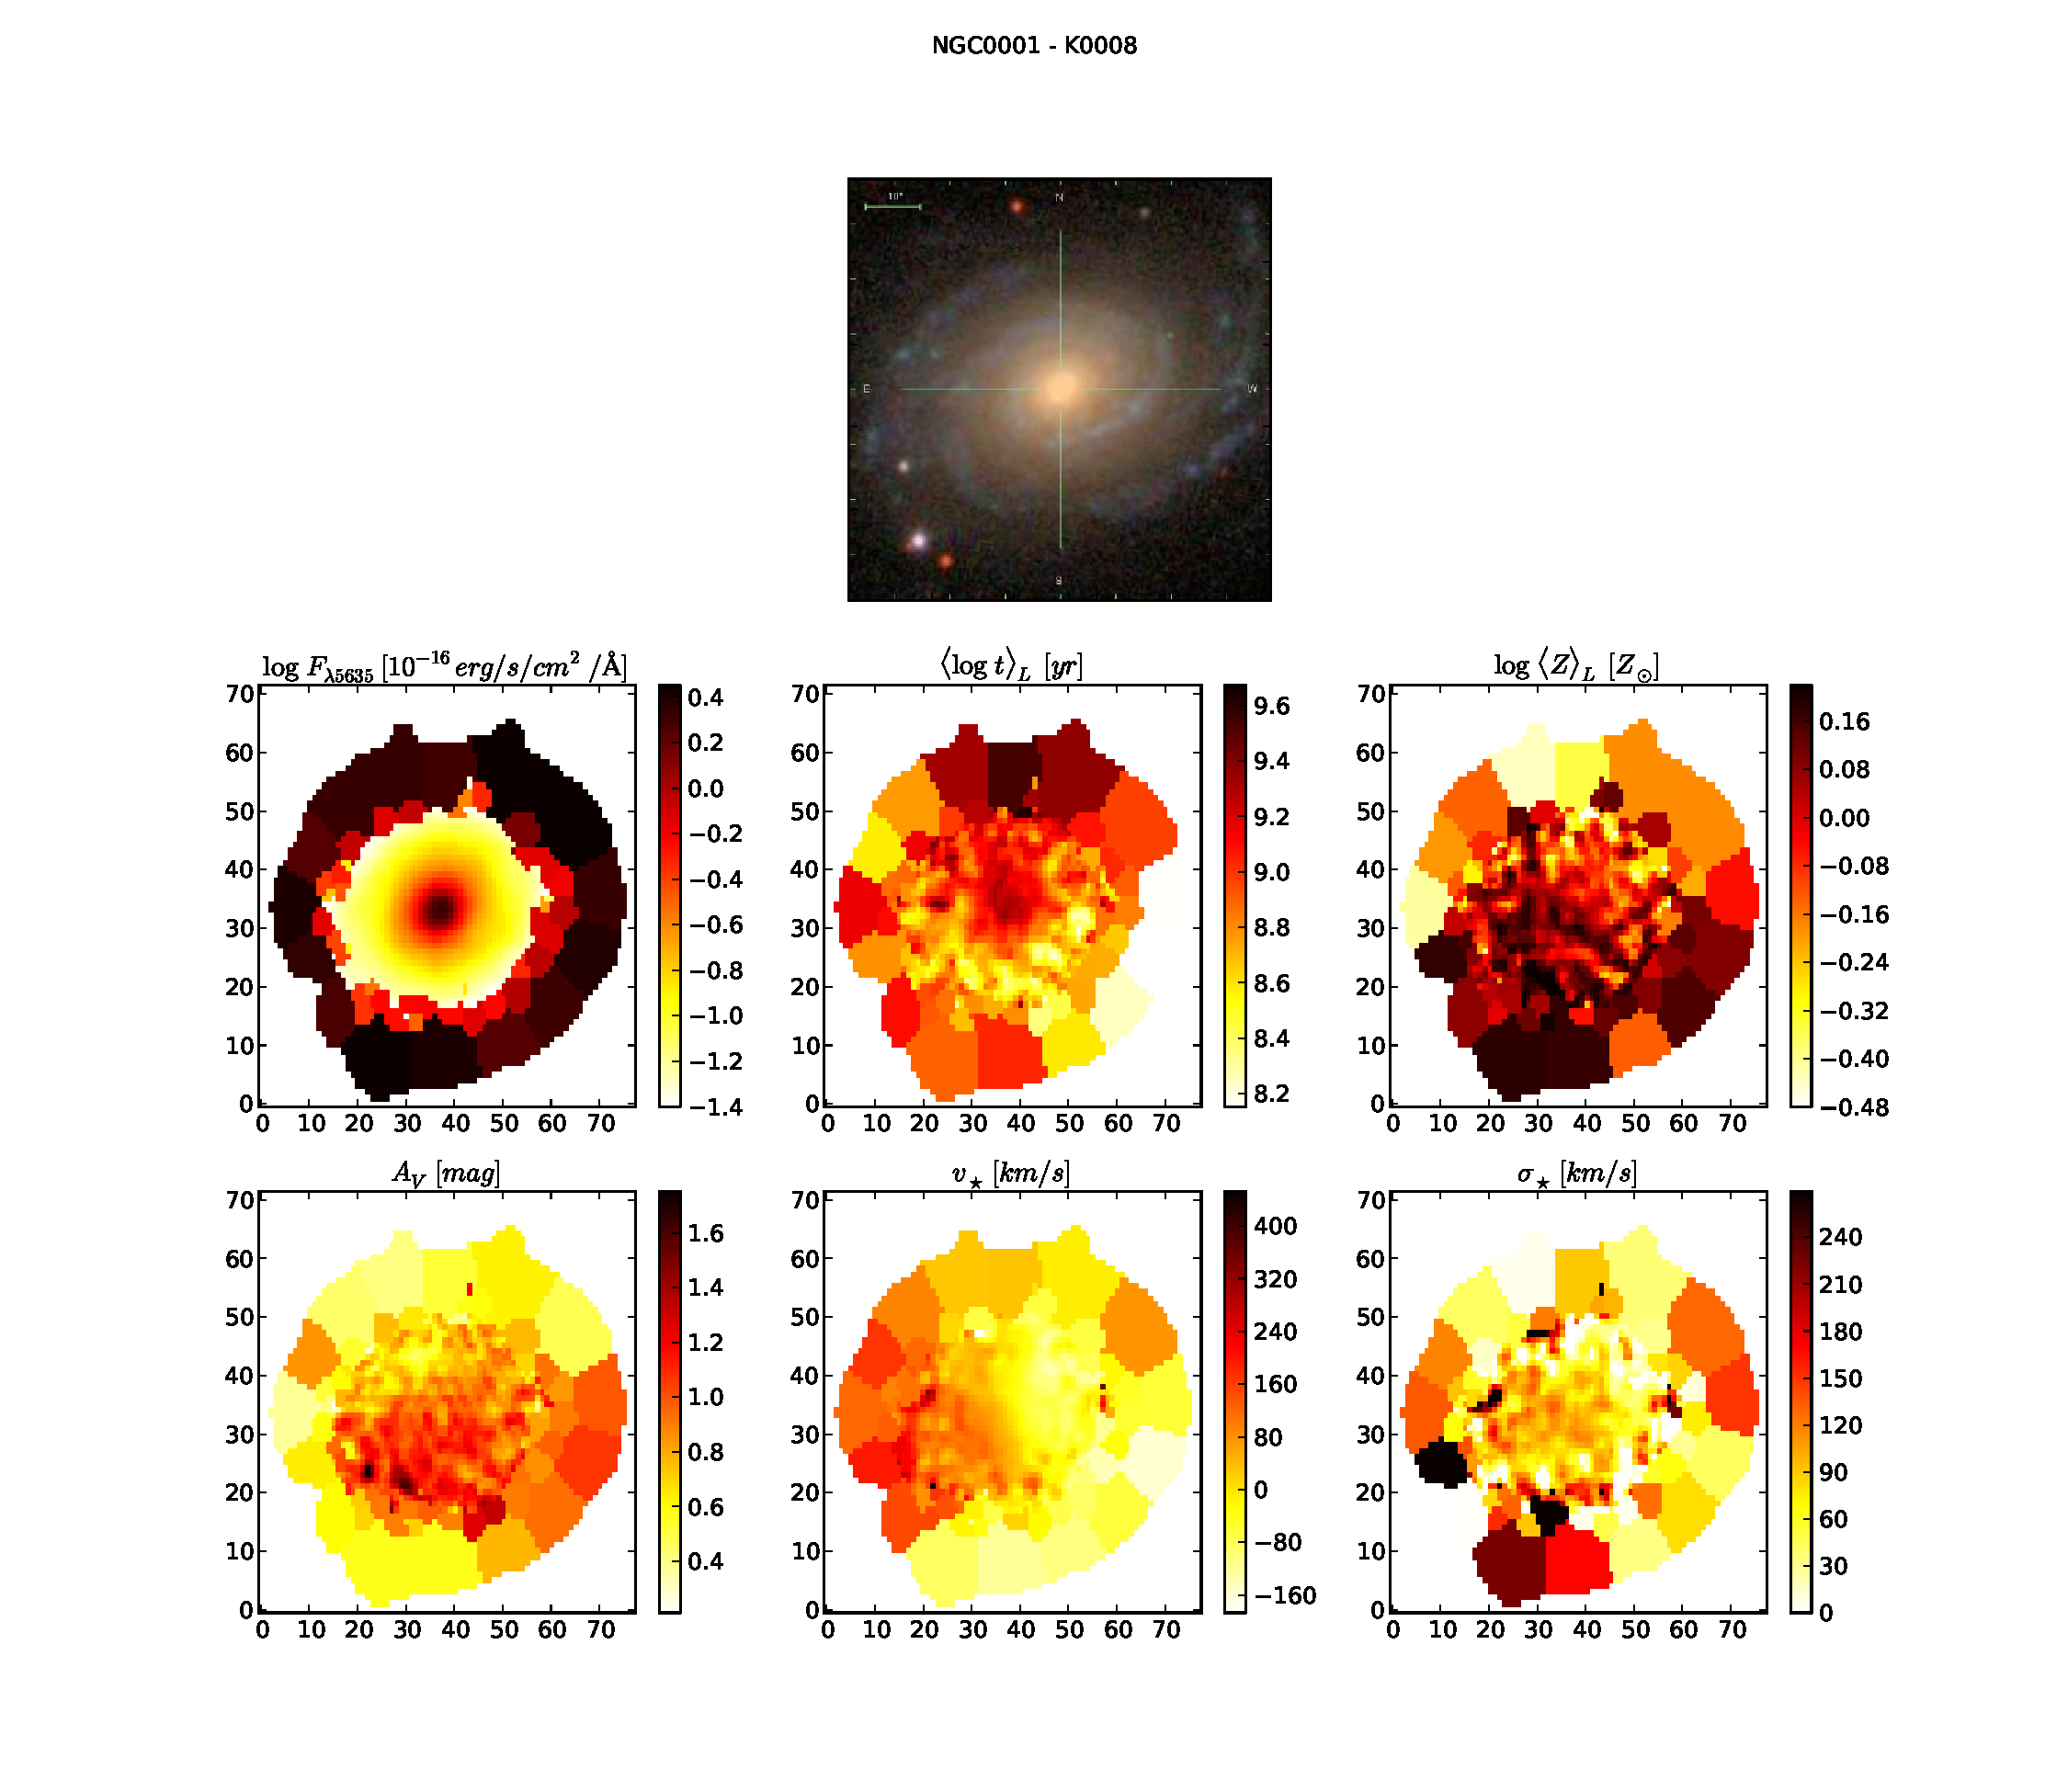
\includegraphics[width=1.\textwidth]{figuras/K0008-apresent.pdf}
    \caption[Propriedades f\'isicas da gal\'axia NGC 0001.]
    {Propriedades físicas da galáxia NGC 0001. Na primeira linha a imagem do SDSS da galáxia. Na primeira imagem da
    segunda linha temos o valor do fluxo observado em 5635 \AA, usado para a normalização dos espectros de cada zona. Da
    segunda imagem da segunda linha em diante temos as propriedades físicas que serão correlacionadas com as PCs. São
    elas: $\meanL{\log\ t}$, $\log\ \meanL{Z}$, $A_V$, $v_{\star}$, $\sigma_{\star}$.}
    \label{fig:K0008apresent}
\end{figure}

\begin{figure}
    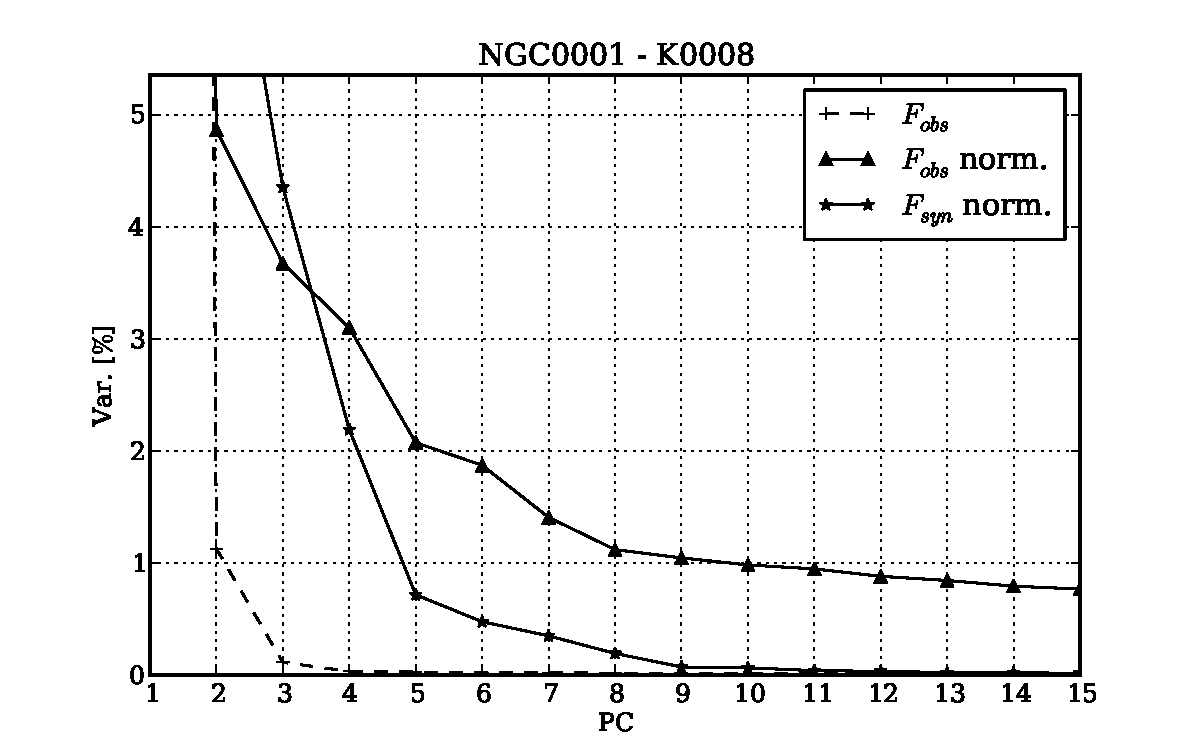
\includegraphics[height=0.33\textheight]{figuras/K0008-screetest.pdf}
    \caption[Scree test comparativo entre 3 PCAs - NGC 0001.]
    {Scree test para 3 análises PCA da galáxia NGC 0001 (CALIFA 8). Com marcações de triângulos vemos as PCs
    resultantes do PCA com os espectros observados normalizados. As variâncias das PCs marcadas com estrela representam
    o PCA com os espectros sintéticos normalizados. Para comparação plotamos as PCs do caso sem normalização usando
    linha pontilhada.}
    \label{fig:K0008scree}
\end{figure}

\begin{figure}
    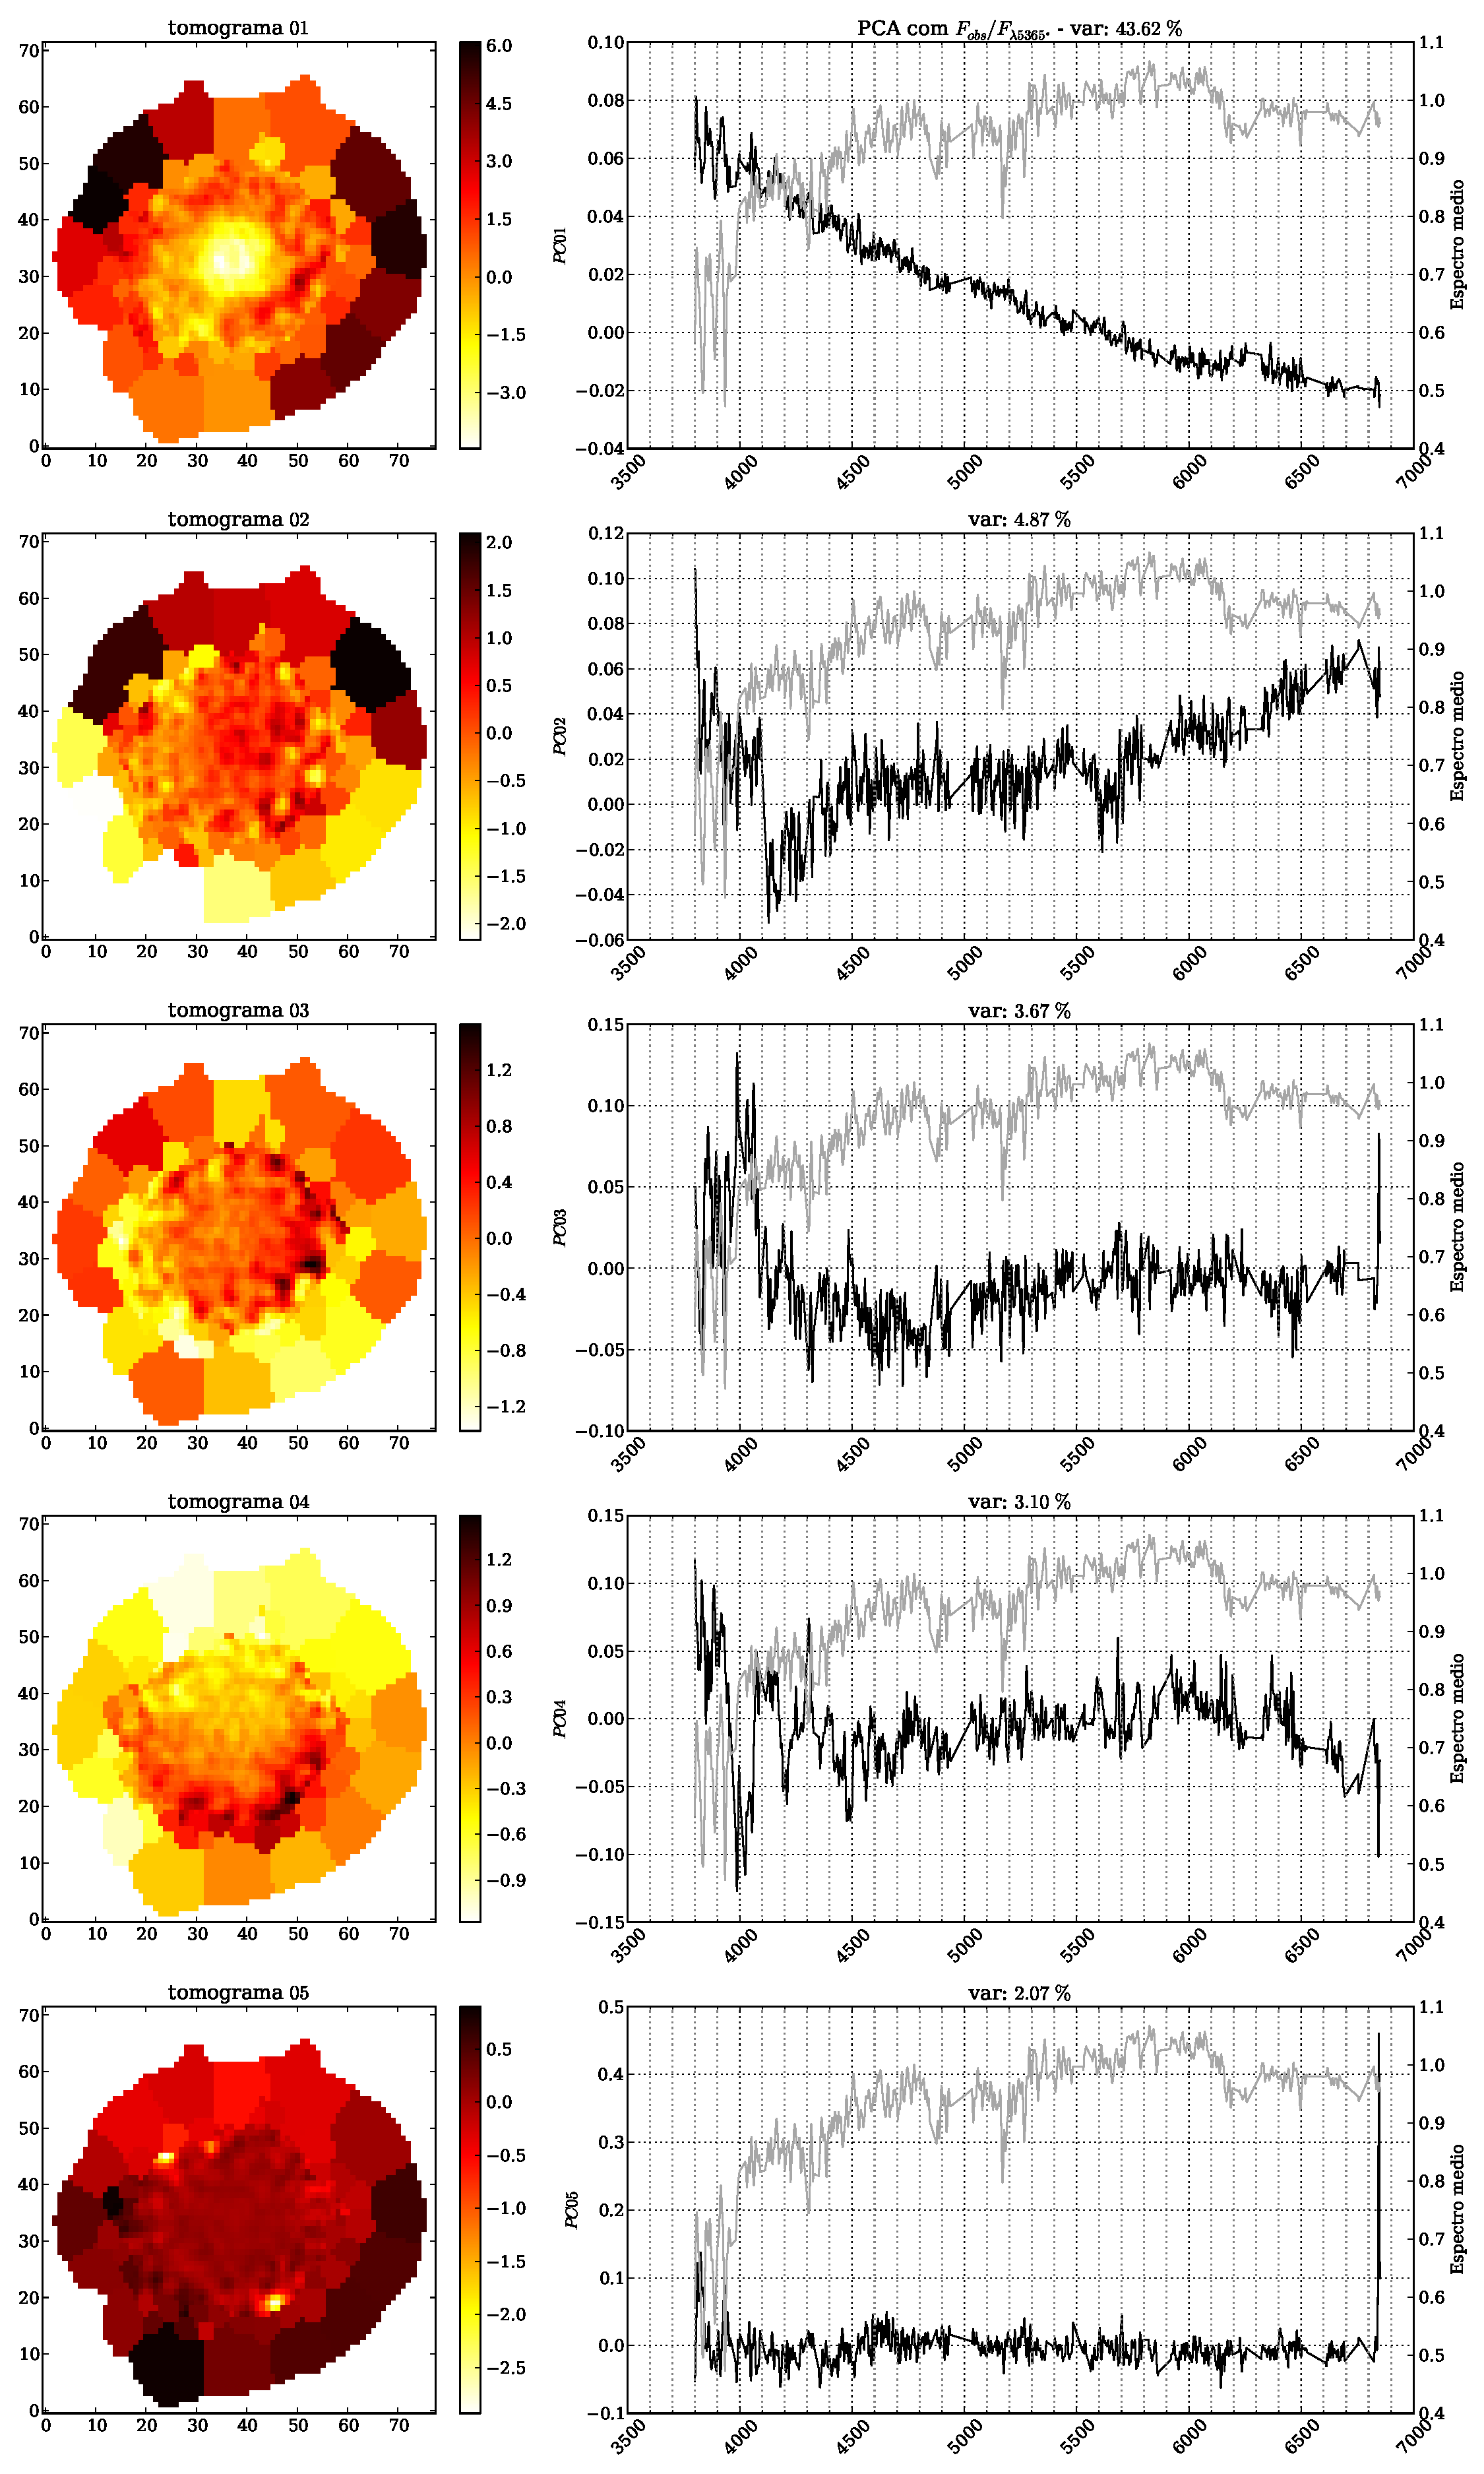
\includegraphics[width=0.8\textwidth]{figuras/K0008-tomo-obs-norm.pdf}
    \caption[Tomogramas de 1 a 5 para o cubo $f_{obs}$ - NGC 0001.]
    {Cinco primeiras PCs (e seus respectivos tomogramas) resultantes da Tomografia PCA aplicado aos espectros
    observados com normalização da galáxia NGC 0001.}
    \label{fig:K0008tomofobsnorm}
\end{figure}

\begin{figure}
    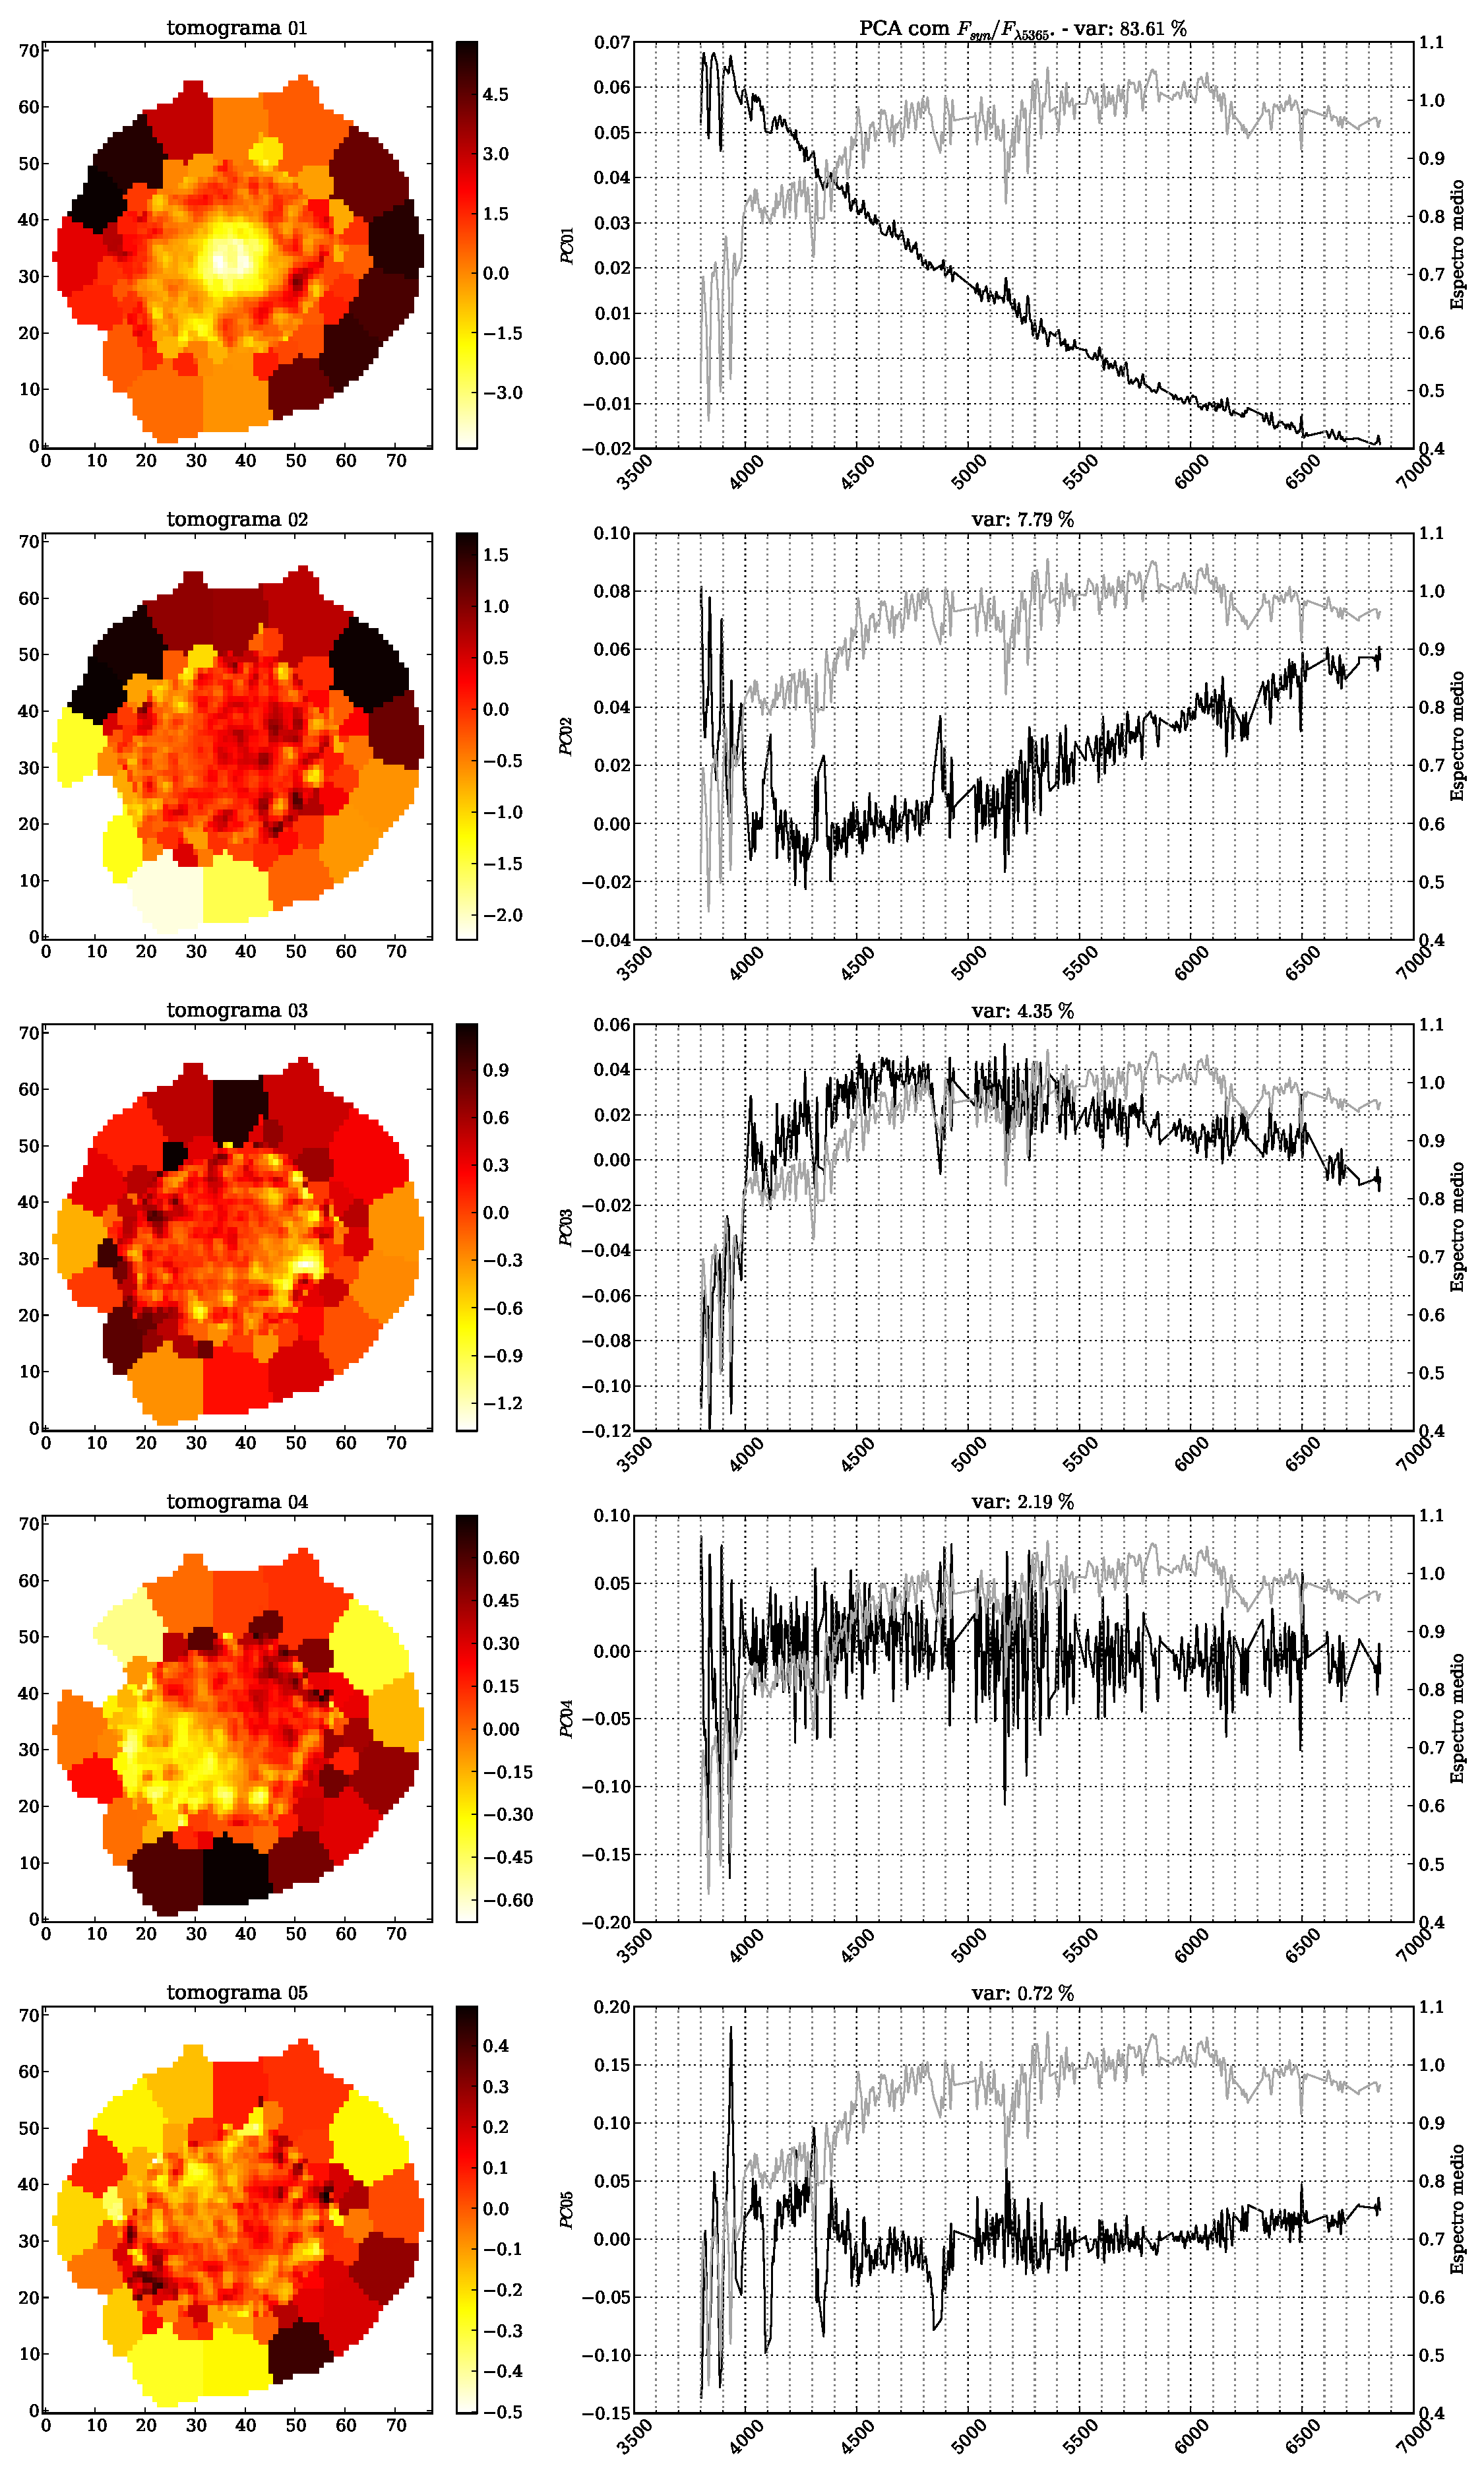
\includegraphics[width=0.8\textwidth]{figuras/K0008-tomo-syn-norm.pdf}
    \caption[Tomogramas de 1 a 5 para o cubo $f_{syn}$ - NGC 0001.]
    {Cinco primeiras PCs (e seus respectivos tomogramas) resultantes da Tomografia PCA aplicado aos espectros
    sintéticos com normalização da galáxia NGC 0001.}
    \label{fig:K0008tomofsynnorm}
\end{figure}

\begin{figure}
    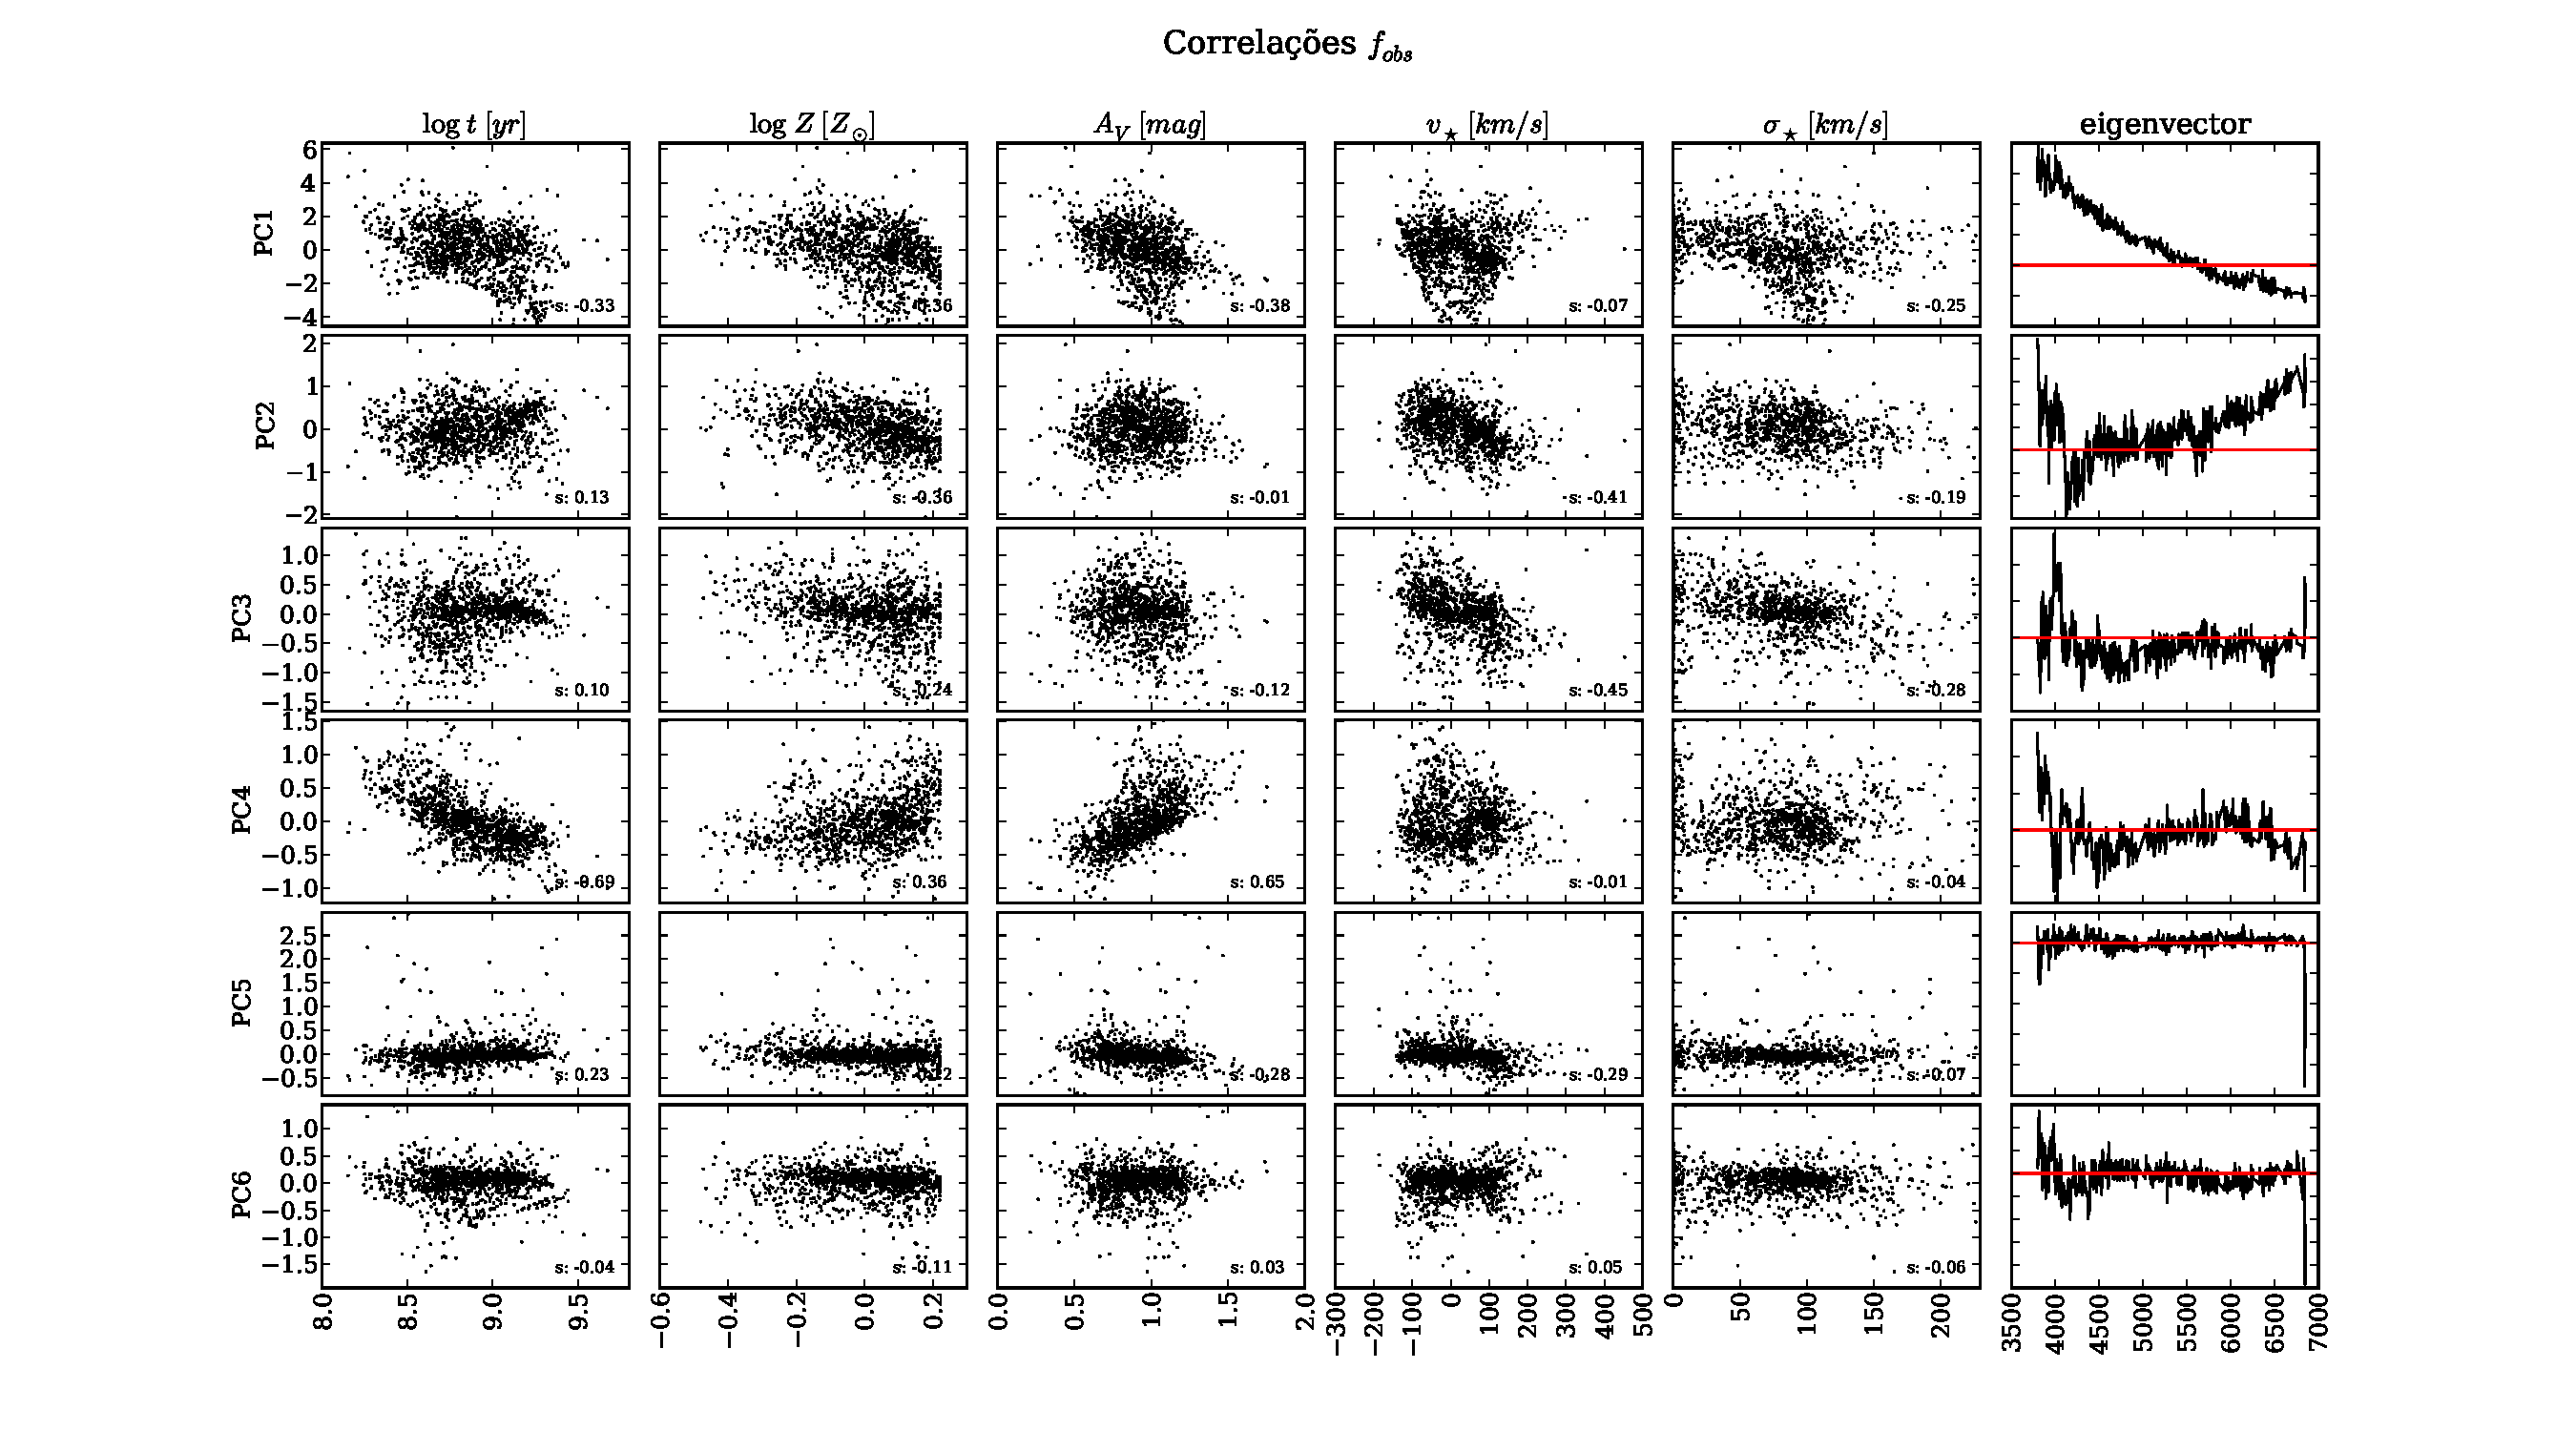
\includegraphics[width=1.2\textwidth, angle=-90]{figuras/K0008-correl-f_obs_norm-PCvsPhys.pdf}
	\caption[Correlações PCs vs. par\^ametros f\'isicos - $f_{obs}$ - NGC 0001]
    {Correlações entre os pesos por zona das seis primeiras PCs do PCA feito para o cubo com os espectros observados
    normalizados e cinco parâmetros físicos. Pela ordem de colunas da esquerda para direita temos \meanL{\log\ t},
    $\log\ \meanL{Z}$, $A_V$, $v_{\star}$, $\sigma_{\star}$. Na última coluna temos o autoespectro para ajudar na
    visualização. A linha em vermelho no gráfico do autoespectro serve para identificar o zero. O número dentro de cada
    gráfico é o coeficiente de correlação de Spearman.}
    \label{fig:K0008correfobsnorm}
\end{figure}

\begin{figure}
    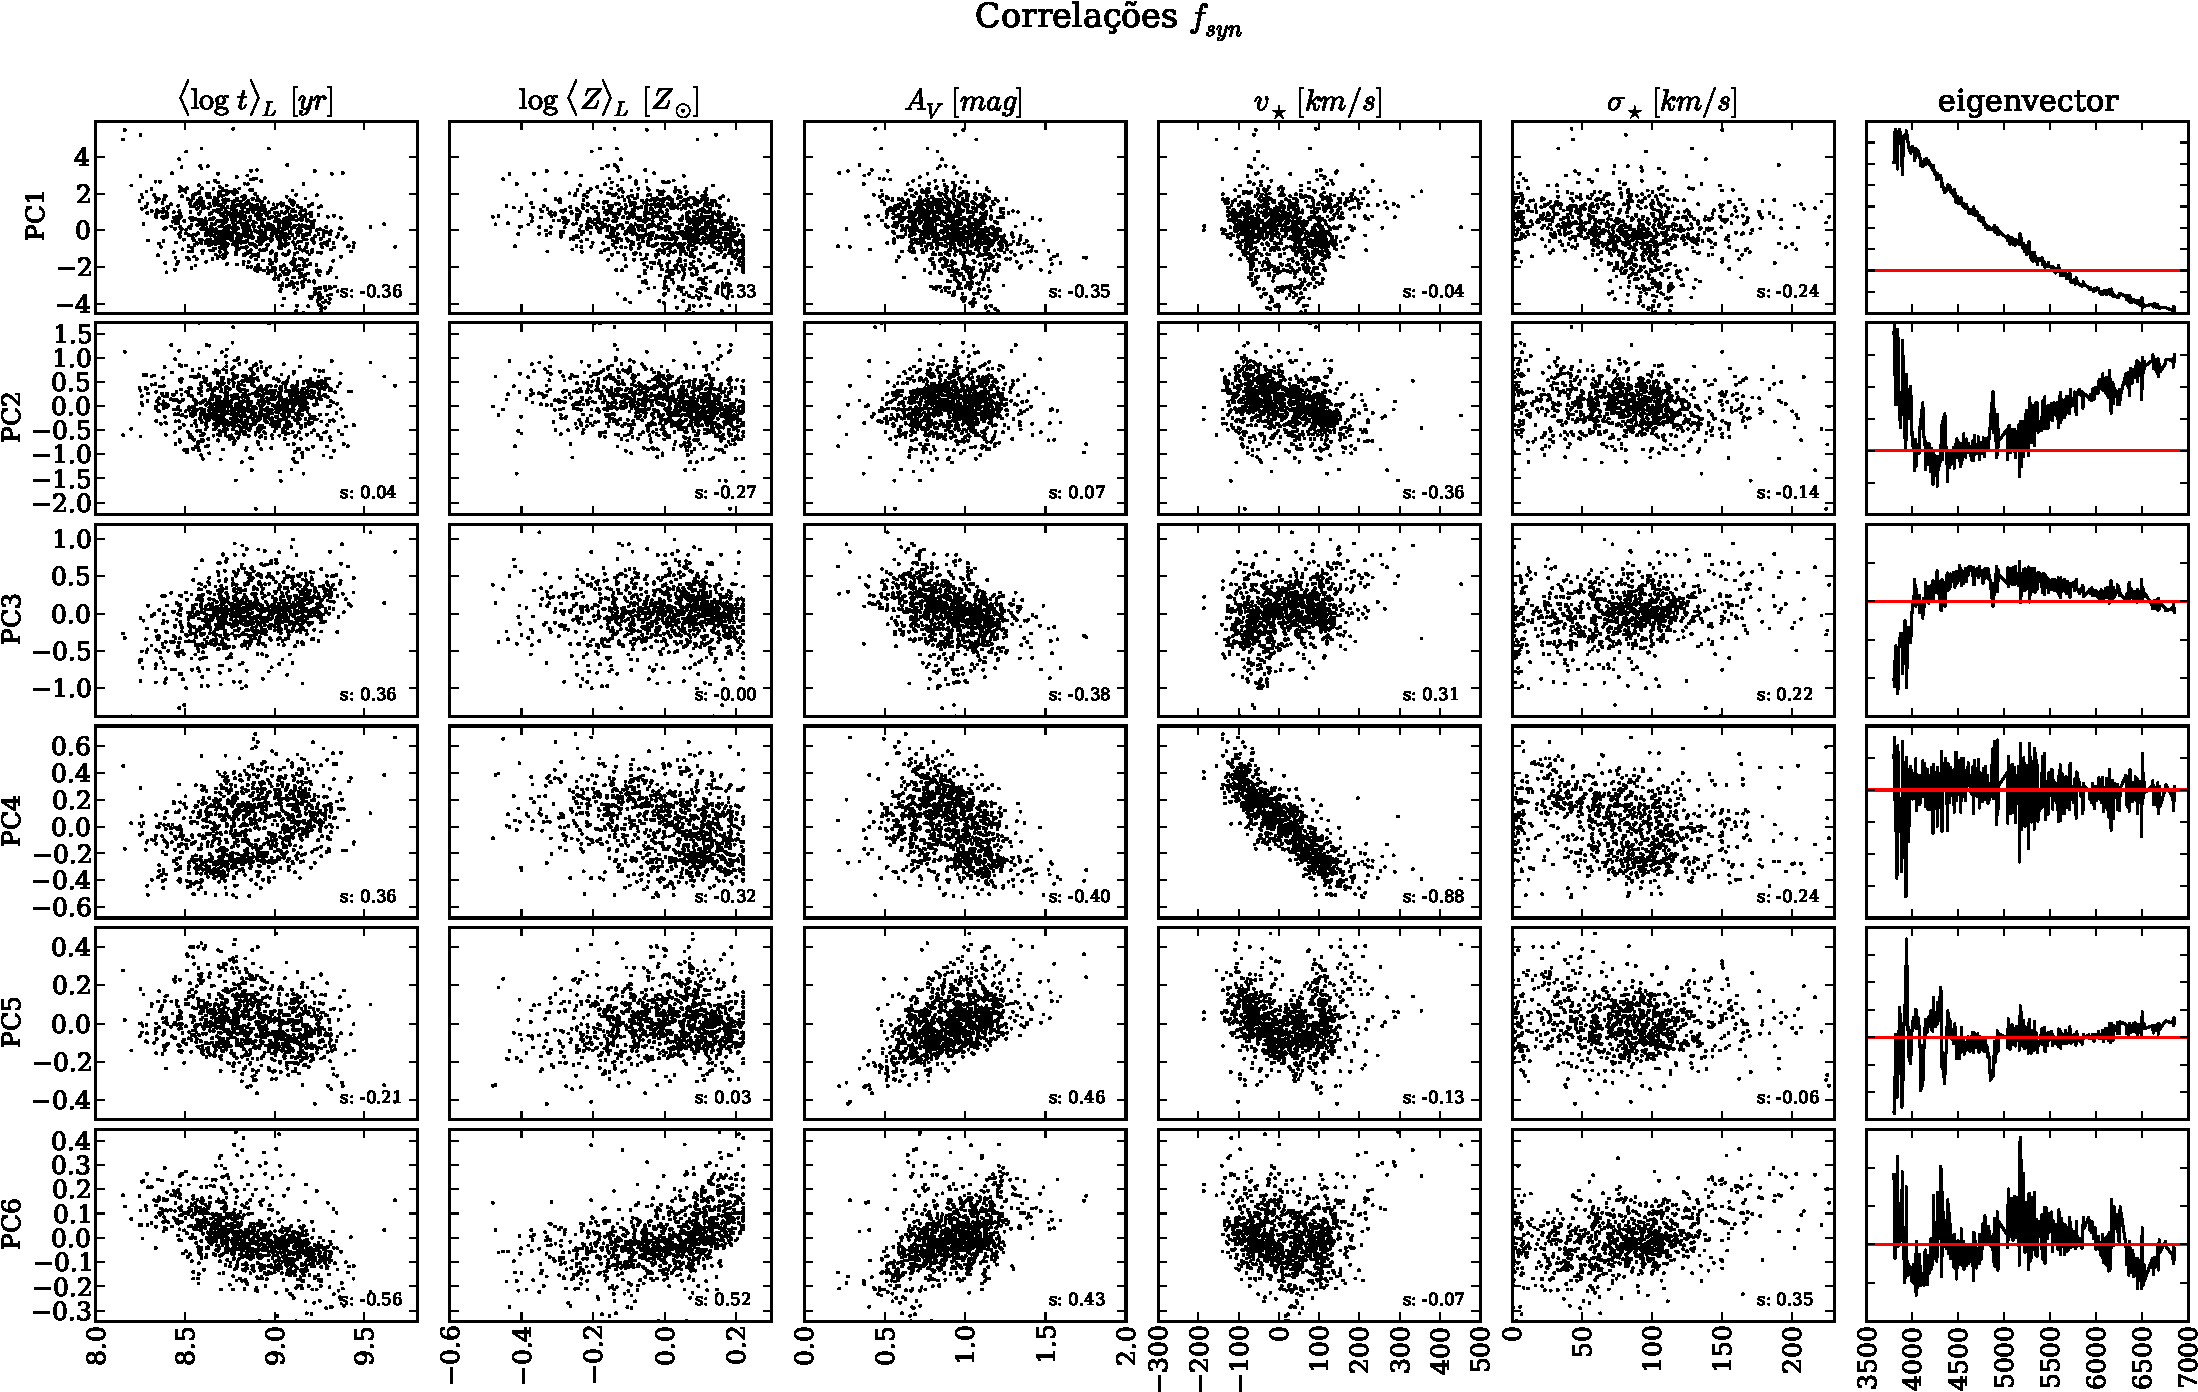
\includegraphics[width=1.2\textwidth, angle=-90]{figuras/K0008-correl-f_syn_norm-PCvsPhys.pdf}
	\caption[Correlações PCs vs. par\^ametros f\'isicos - $f_{syn}$ - NGC 0001]
    {Correlações entre os pesos por zona das seis primeiras PCs do PCA feito para o cubo com os espectros sintéticos
    normalizados e cinco parâmetros físicos.q Pela ordem de colunas da esquerda para direita temos \meanL{\log\ t},
    $\log\ \meanL{Z}$, $A_V$, $v_{\star}$, $\sigma_{\star}$. Na última coluna temos o autoespectro para ajudar na
    visualização. A linha em vermelho no gráfico do autoespectro serve para identificar o zero. O número dentro de cada
    gráfico é o coeficiente de correlação de Spearman.}
    \label{fig:K0008correfsynnorm}
\end{figure}

\subsection{NGC 0776 - CALIFA 73}

A galáxia espiral barrada NGC 0776 é apresentada na Figura \ref{fig:K0073apresent}. A análise com o \starlight revela
populações mais jovens nos braços espirais, uma populacao velha na região da barra e levemente mais jovem no núcleo. A
imagem de $A_V$ mostra que a poeira se concentra no núcleo e nos braços. O campo de velocidade mostra pequenos valores
de $v_\star$, o que não é supreendente dado que a galáxias está praticamente {\em face-on}.

A análise da variância percentual de cada componente através do {\em scree test} (Figura \ref{fig:K0073scree}) segue o
mesmo padrão de todas apresentadas até agora, sempre com a convergência ao zero de variância seguindo a ordem primeiro
$F_{obs}$, depois $f_{syn}$ e por último $f_{obs}$. Veremos que todos os {\em scree tests} avaliados seguem esse mesmo
padrão assintótico, independentemente do tipo morfológico da galáxia.

Ambas análises para diferentes configurações resultam na primeira PC muito semelhante (Figuras
\ref{fig:K0073tomofobsnorm} e \ref{fig:K0073tomofsynnorm}) que correlaciona de maneira forte com a idade média (Figuras
\ref{fig:K0073correfobsnorm} e \ref{fig:K0073correfsynnorm}). De fato o tomograma da PC1 se assemelha bastante a imagem
da idade média. A segunda componente para o caso sintético parece carregar informação da série de Balmer (também vista
na PC4) e correlacionar com $A_V$. Já para o caso observado possui melhor correlação com a velocidade estelar. A
informação sobre $A_V$ parece estar melhor representada pela PC3 para o caso observado, diferentemente do caso sintético
que parece conter essa informação de maneira um pouco mais clara na PC4. Vale a pena ressaltar que apesar dessa galáxia
não ter um campo de velocidades muito distribuído, a PC5 para o caso sintético parece ser uma boa sonda dessa
propriedade.

\begin{figure}
    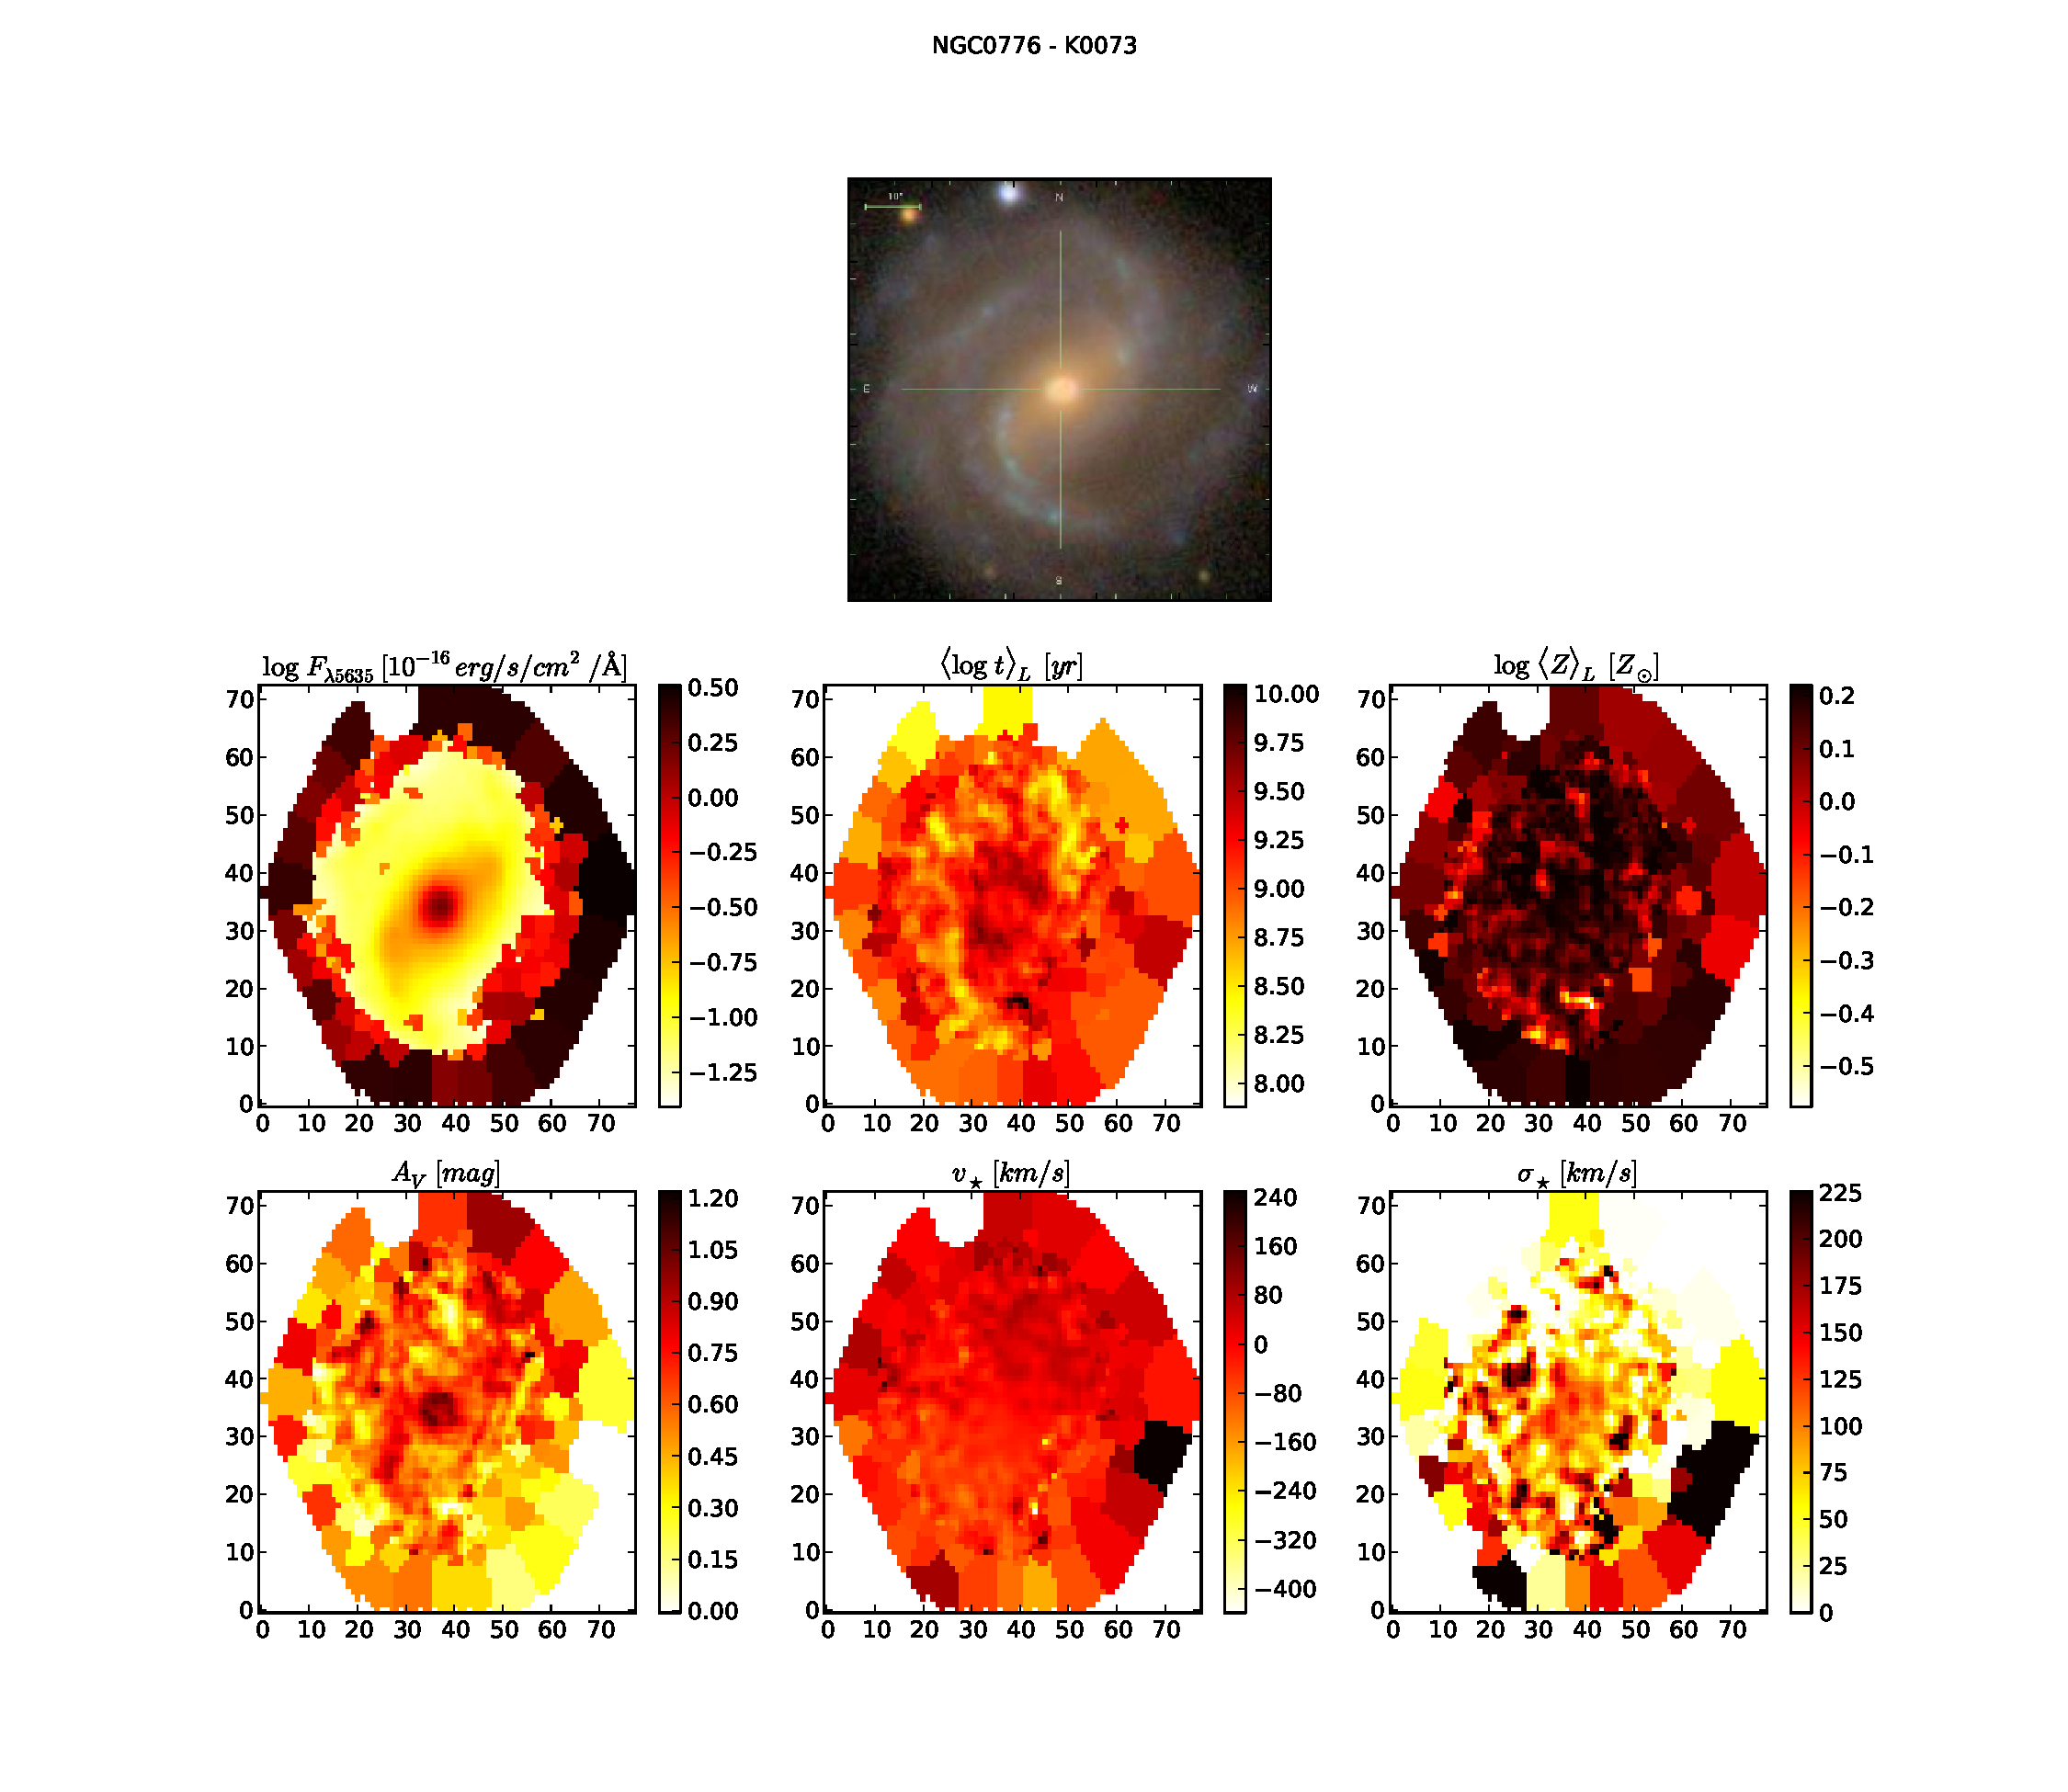
\includegraphics[width=1.\textwidth]{figuras/K0073-apresent.pdf}
    \caption[Propriedades f\'isicas da gal\'axia NGC 0776.]
    {Igual a Figura \ref{fig:K0008apresent} para a galáxia NGC 0776.}
    \label{fig:K0073apresent}
\end{figure}

\begin{figure}
    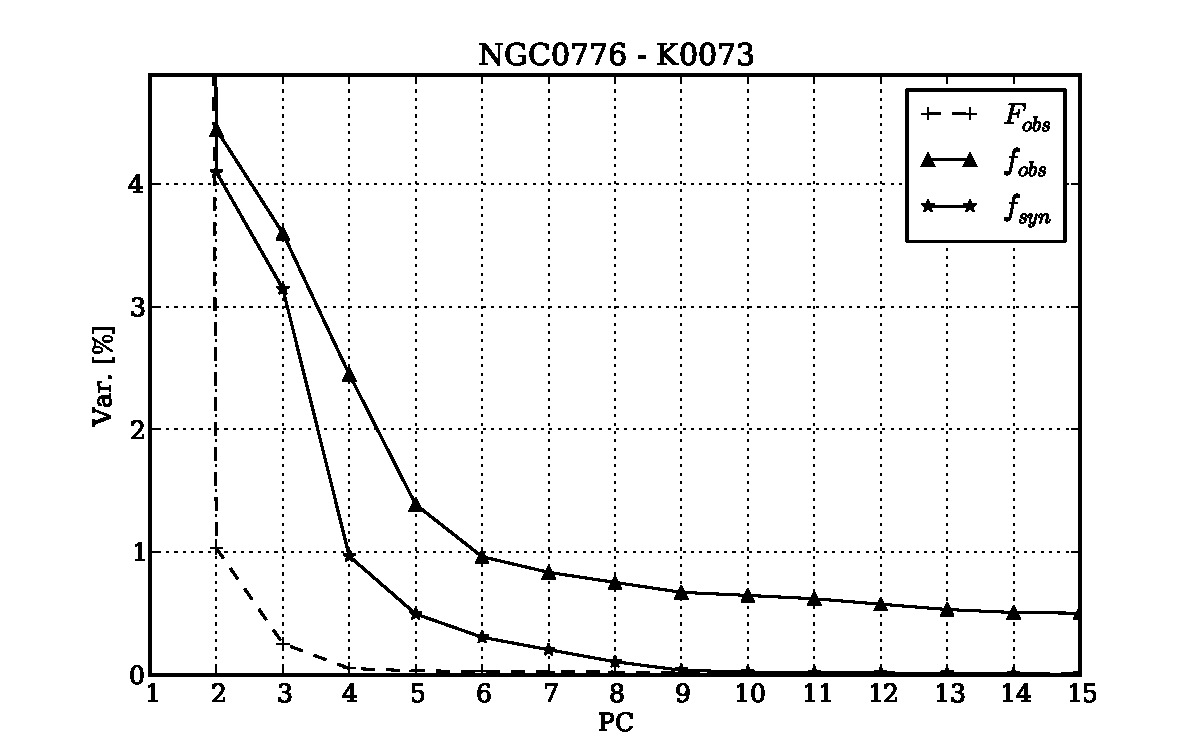
\includegraphics[height=0.33\textheight]{figuras/K0073-screetest.pdf}
    \caption[Scree test comparativo entre 3 PCAs - NGC 0776.]
    {Igual a Figura \ref{fig:K0008scree} para a galáxia NGC 0776.}
    \label{fig:K0073scree}
\end{figure}

\begin{figure}
    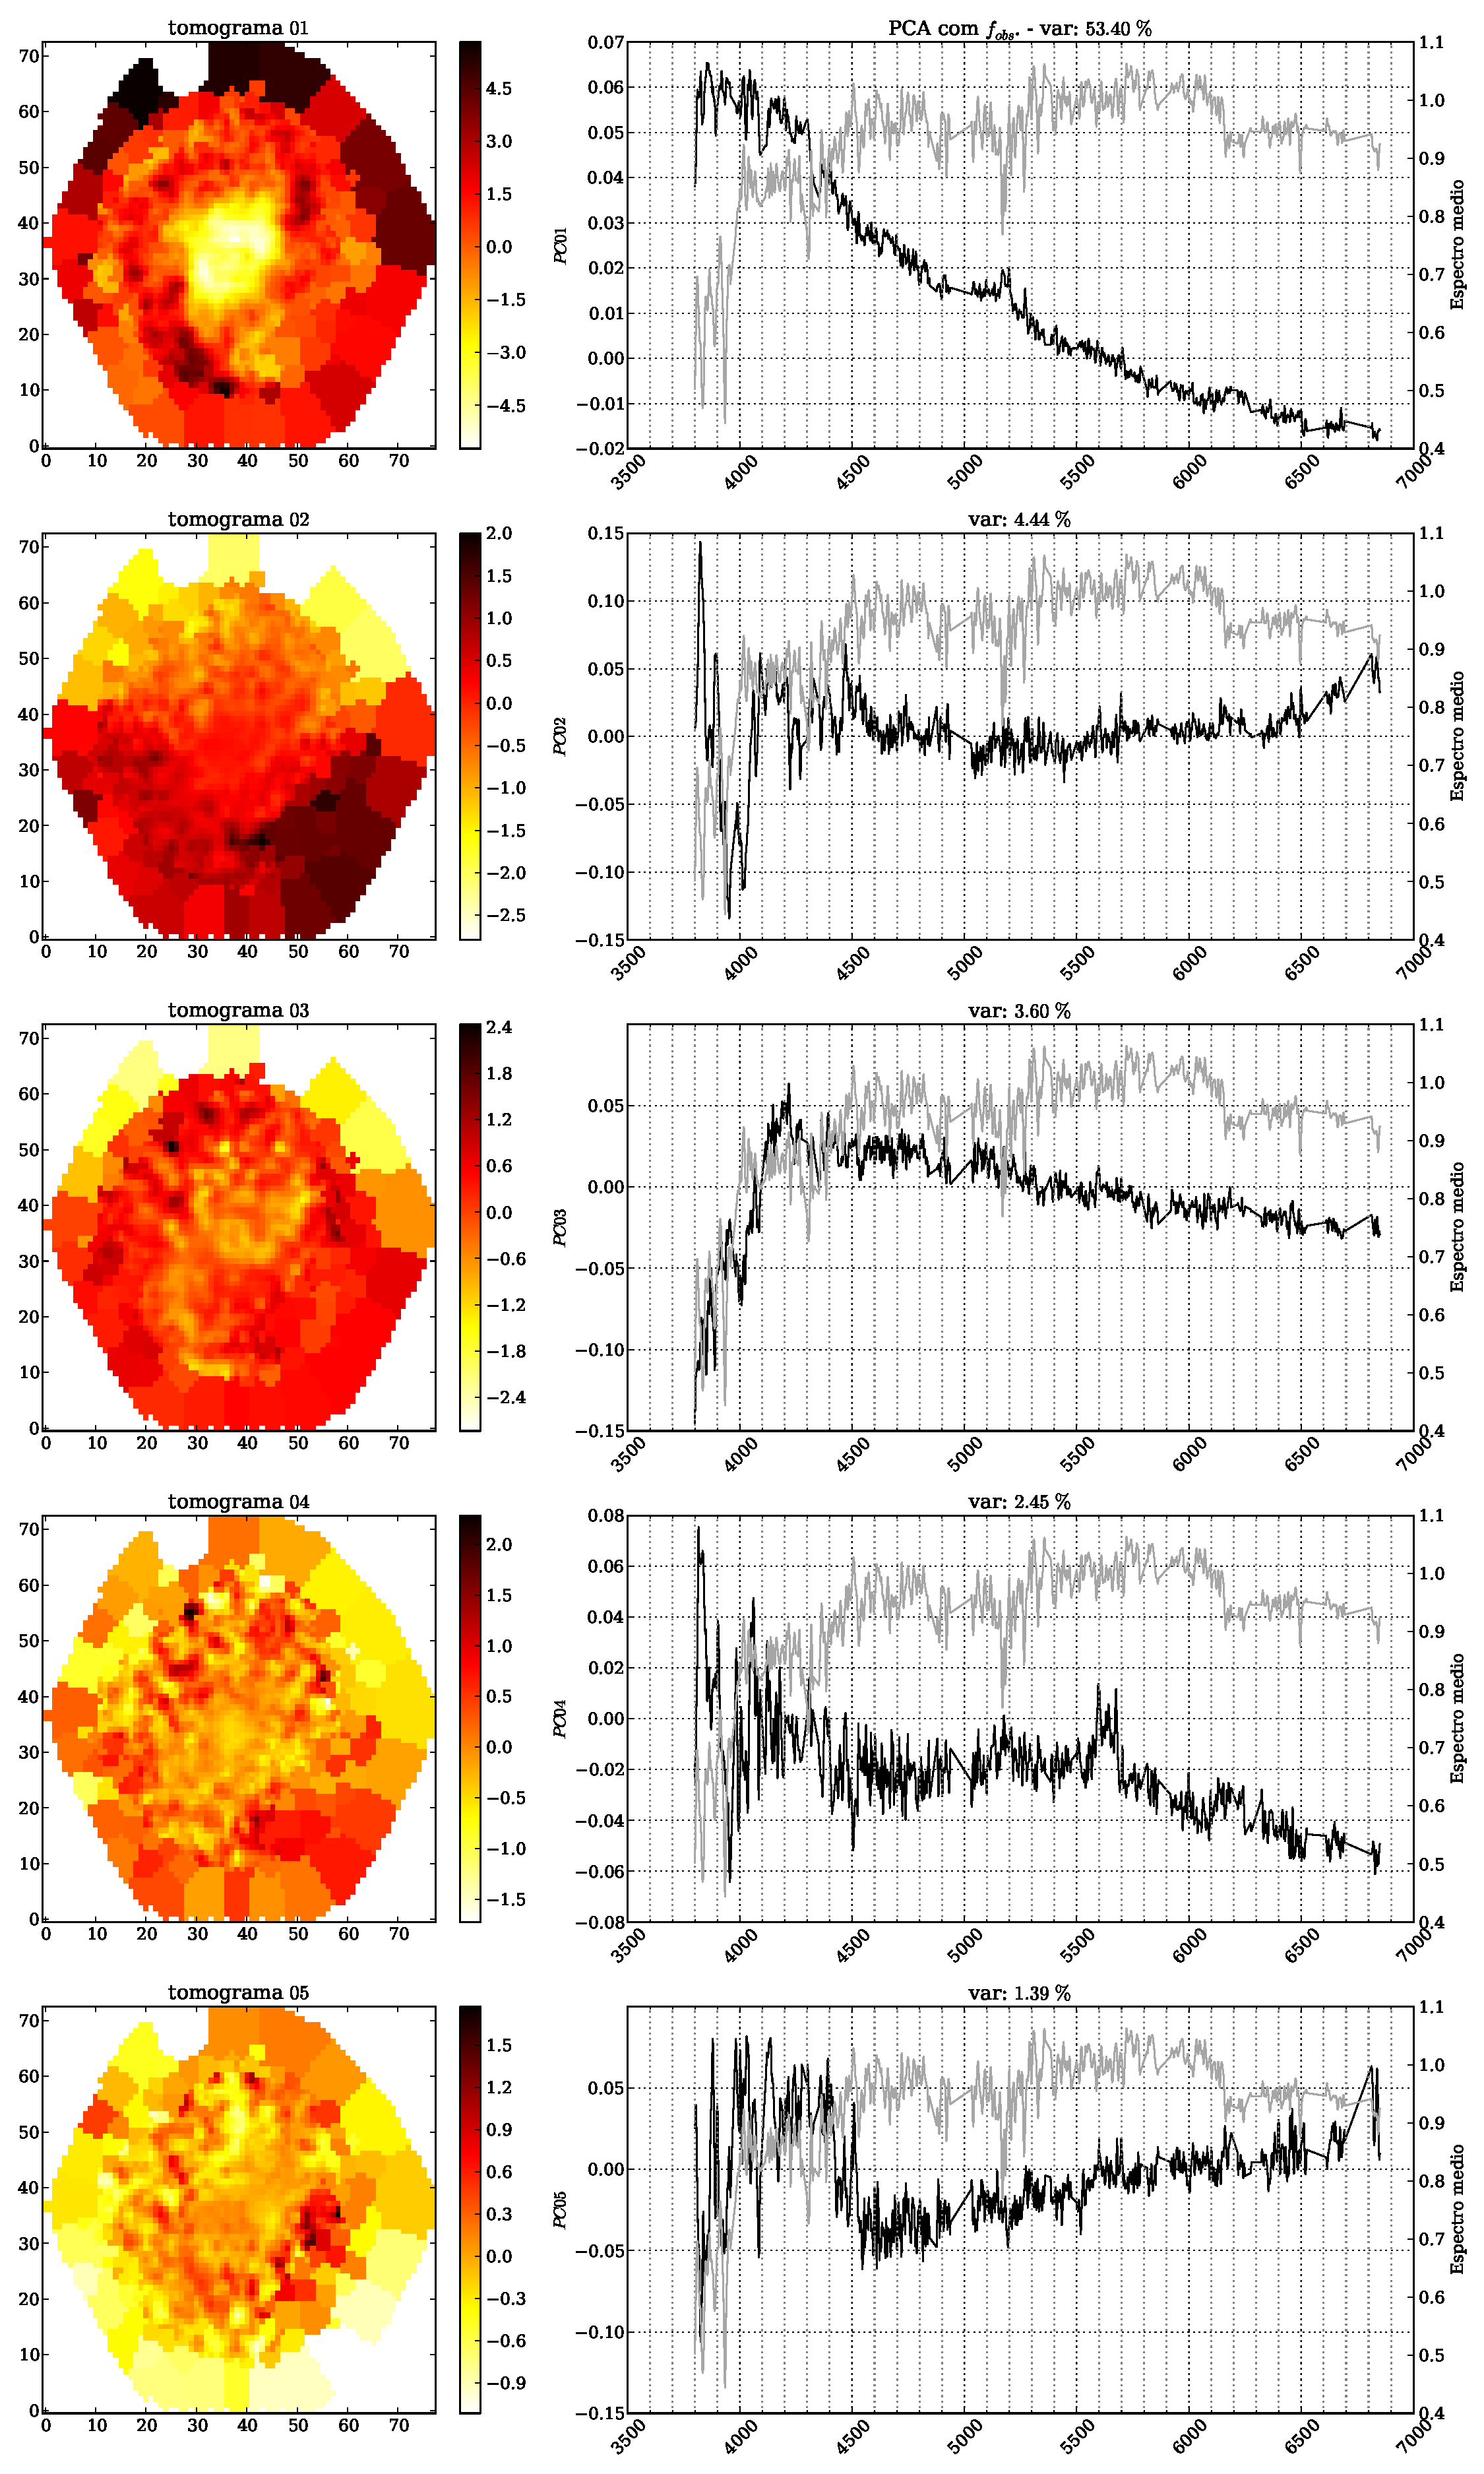
\includegraphics[width=0.8\textwidth]{figuras/K0073-tomo-obs-norm.pdf}
    \caption[Tomogramas de 1 a 5 para o cubo $f_{obs}$ - NGC 0776.]
    {Igual a Figura \ref{fig:K0008tomofobsnorm} para a galáxia NGC 0776.}
    \label{fig:K0073tomofobsnorm}
\end{figure}

\begin{figure}
    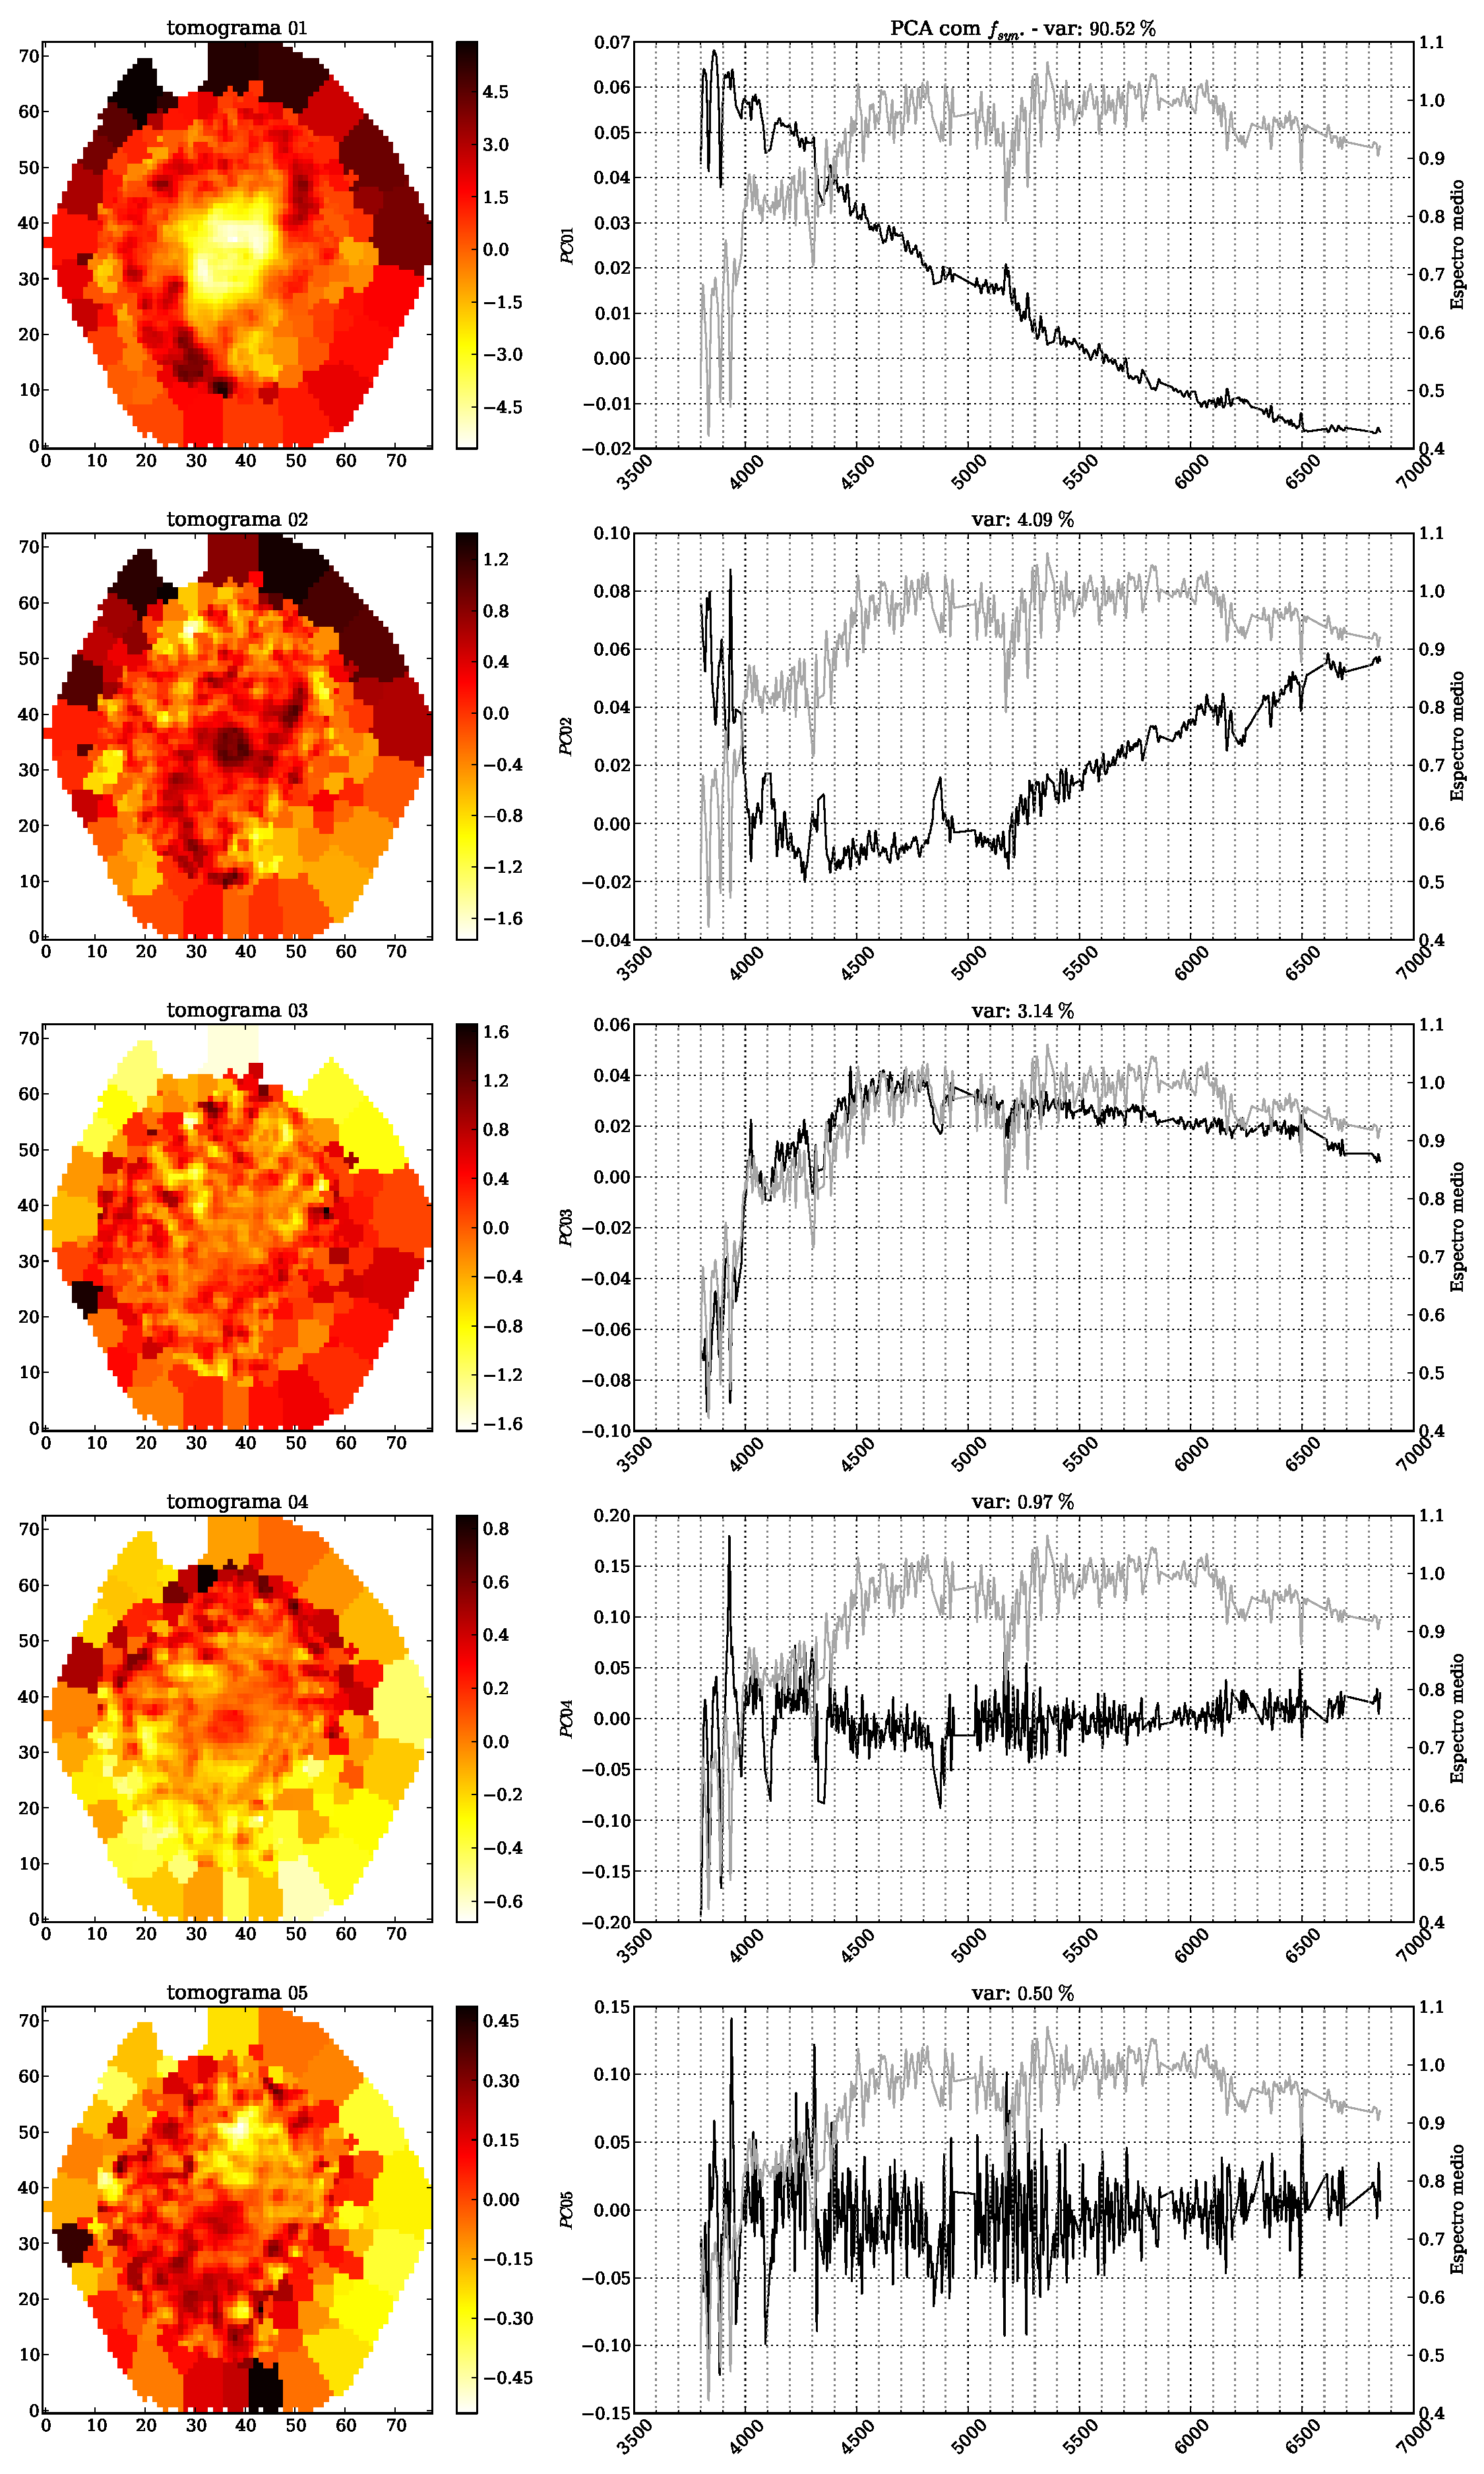
\includegraphics[width=0.8\textwidth]{figuras/K0073-tomo-syn-norm.pdf}
    \caption[Tomogramas de 1 a 5 para o cubo $f_{syn}$ - NGC 0776.]
    {Igual a Figura \ref{fig:K0008tomofsynnorm} para a galáxia NGC 0776.}
    \label{fig:K0073tomofsynnorm}
\end{figure}

\begin{figure}
    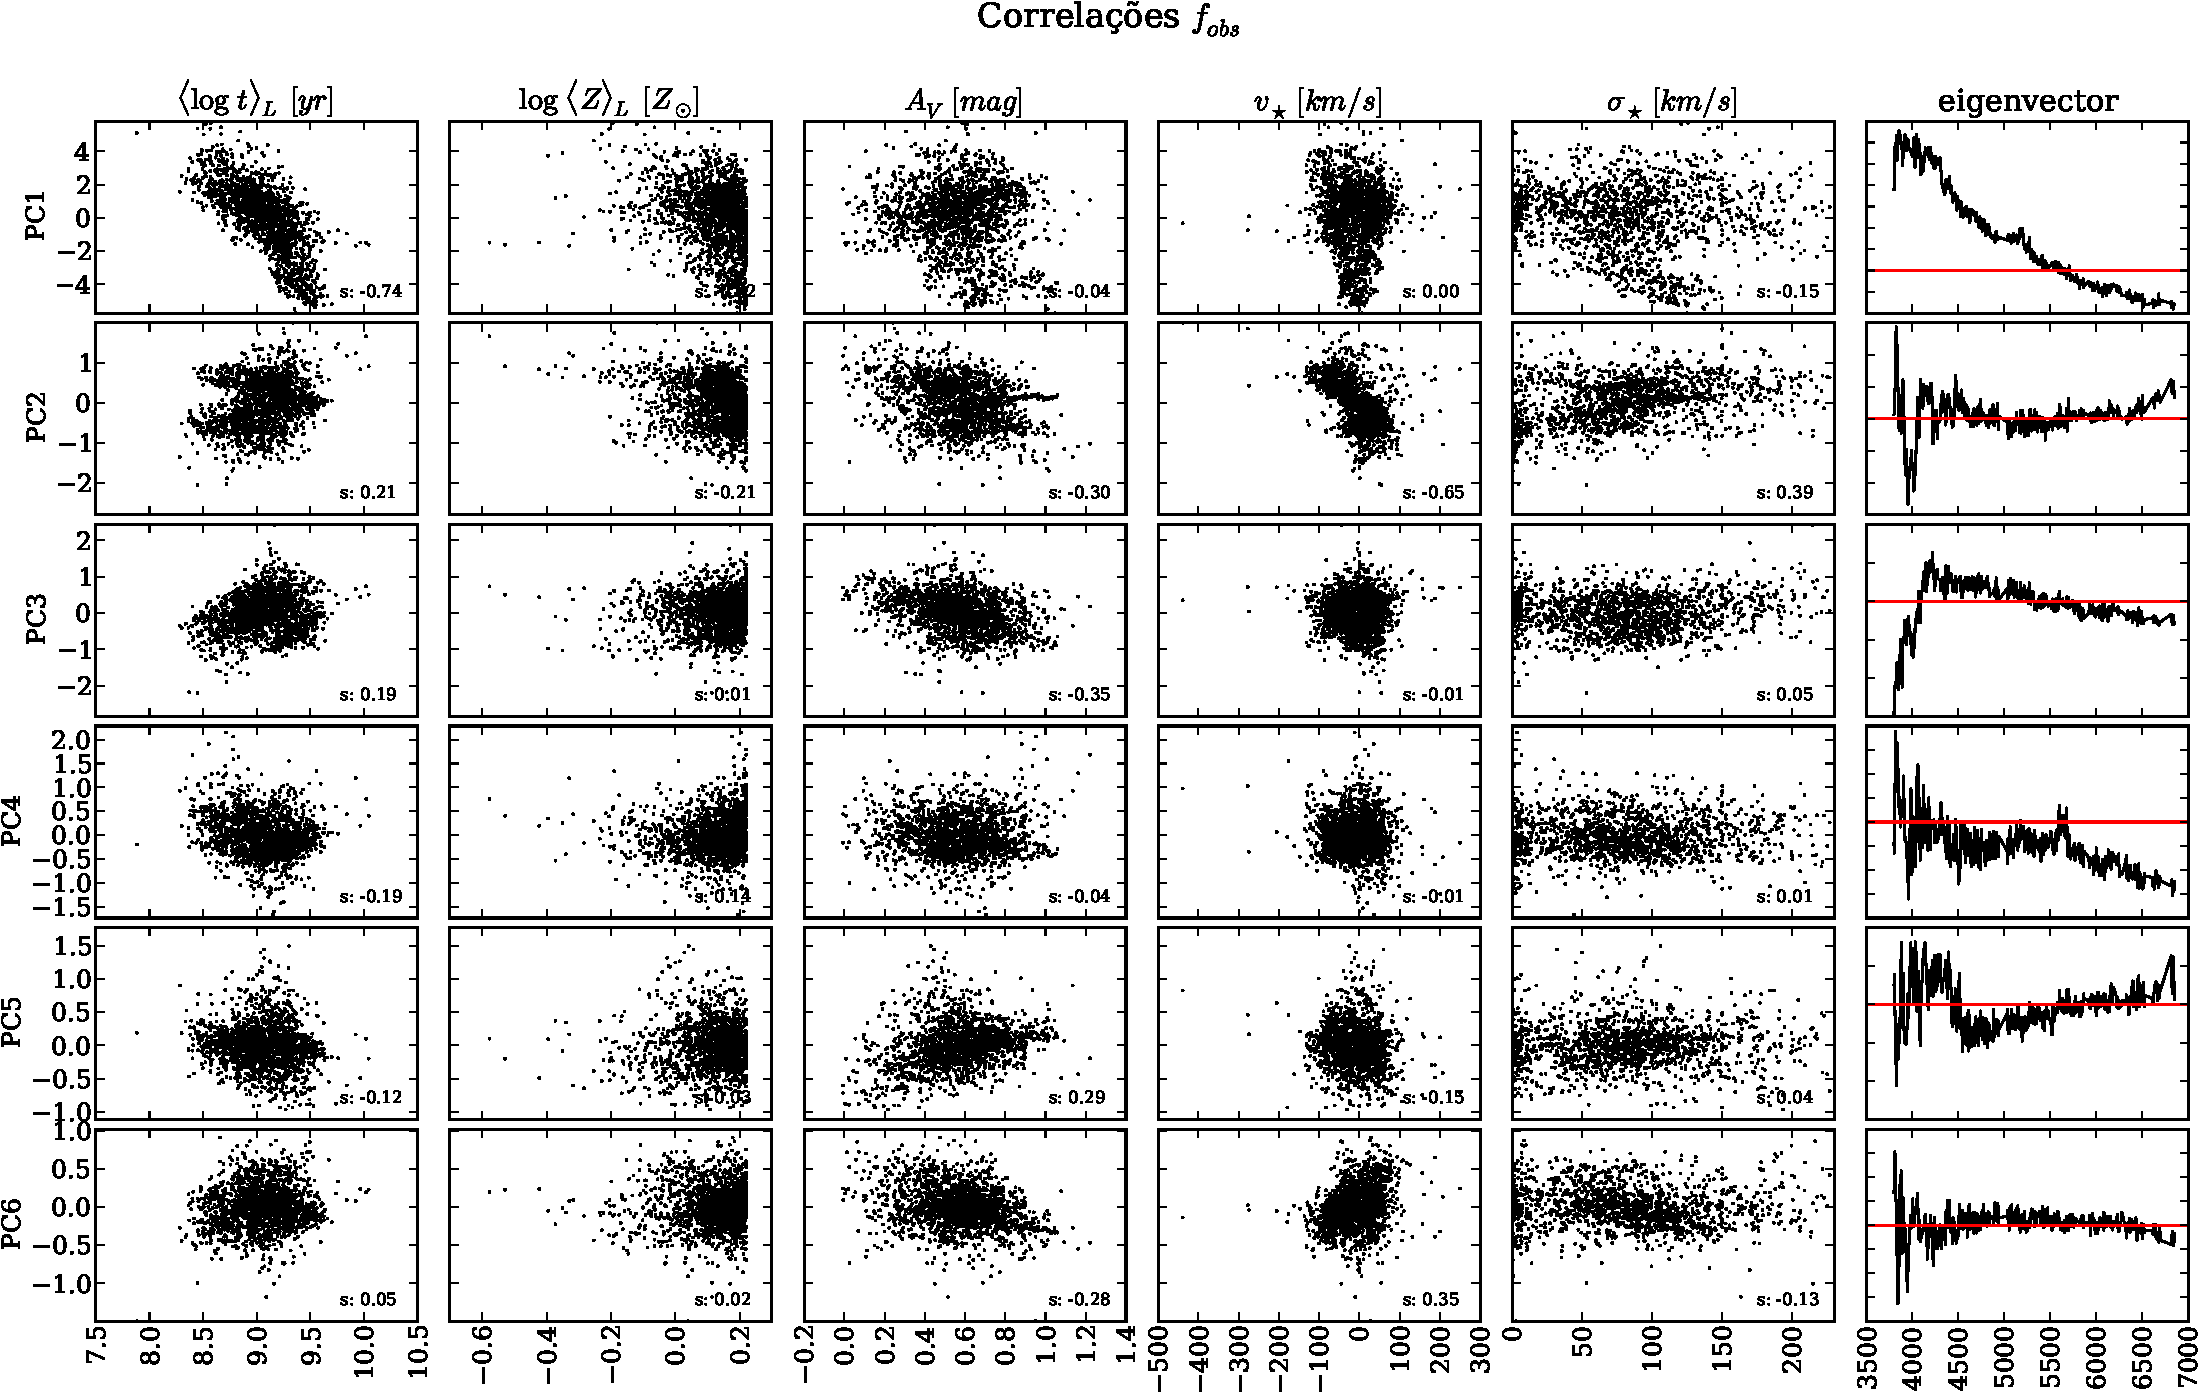
\includegraphics[width=1.2\textwidth, angle=-90]{figuras/K0073-correl-f_obs_norm-PCvsPhys.pdf}
	\caption[Correlações PCs vs. par\^ametros f\'isicos - $f_{obs}$ - NGC 0001]
	{Igual a Figura \ref{fig:K0008correfobsnorm} para a galáxia NGC 0776.}
    \label{fig:K0073correfobsnorm}
\end{figure}

\begin{figure}
    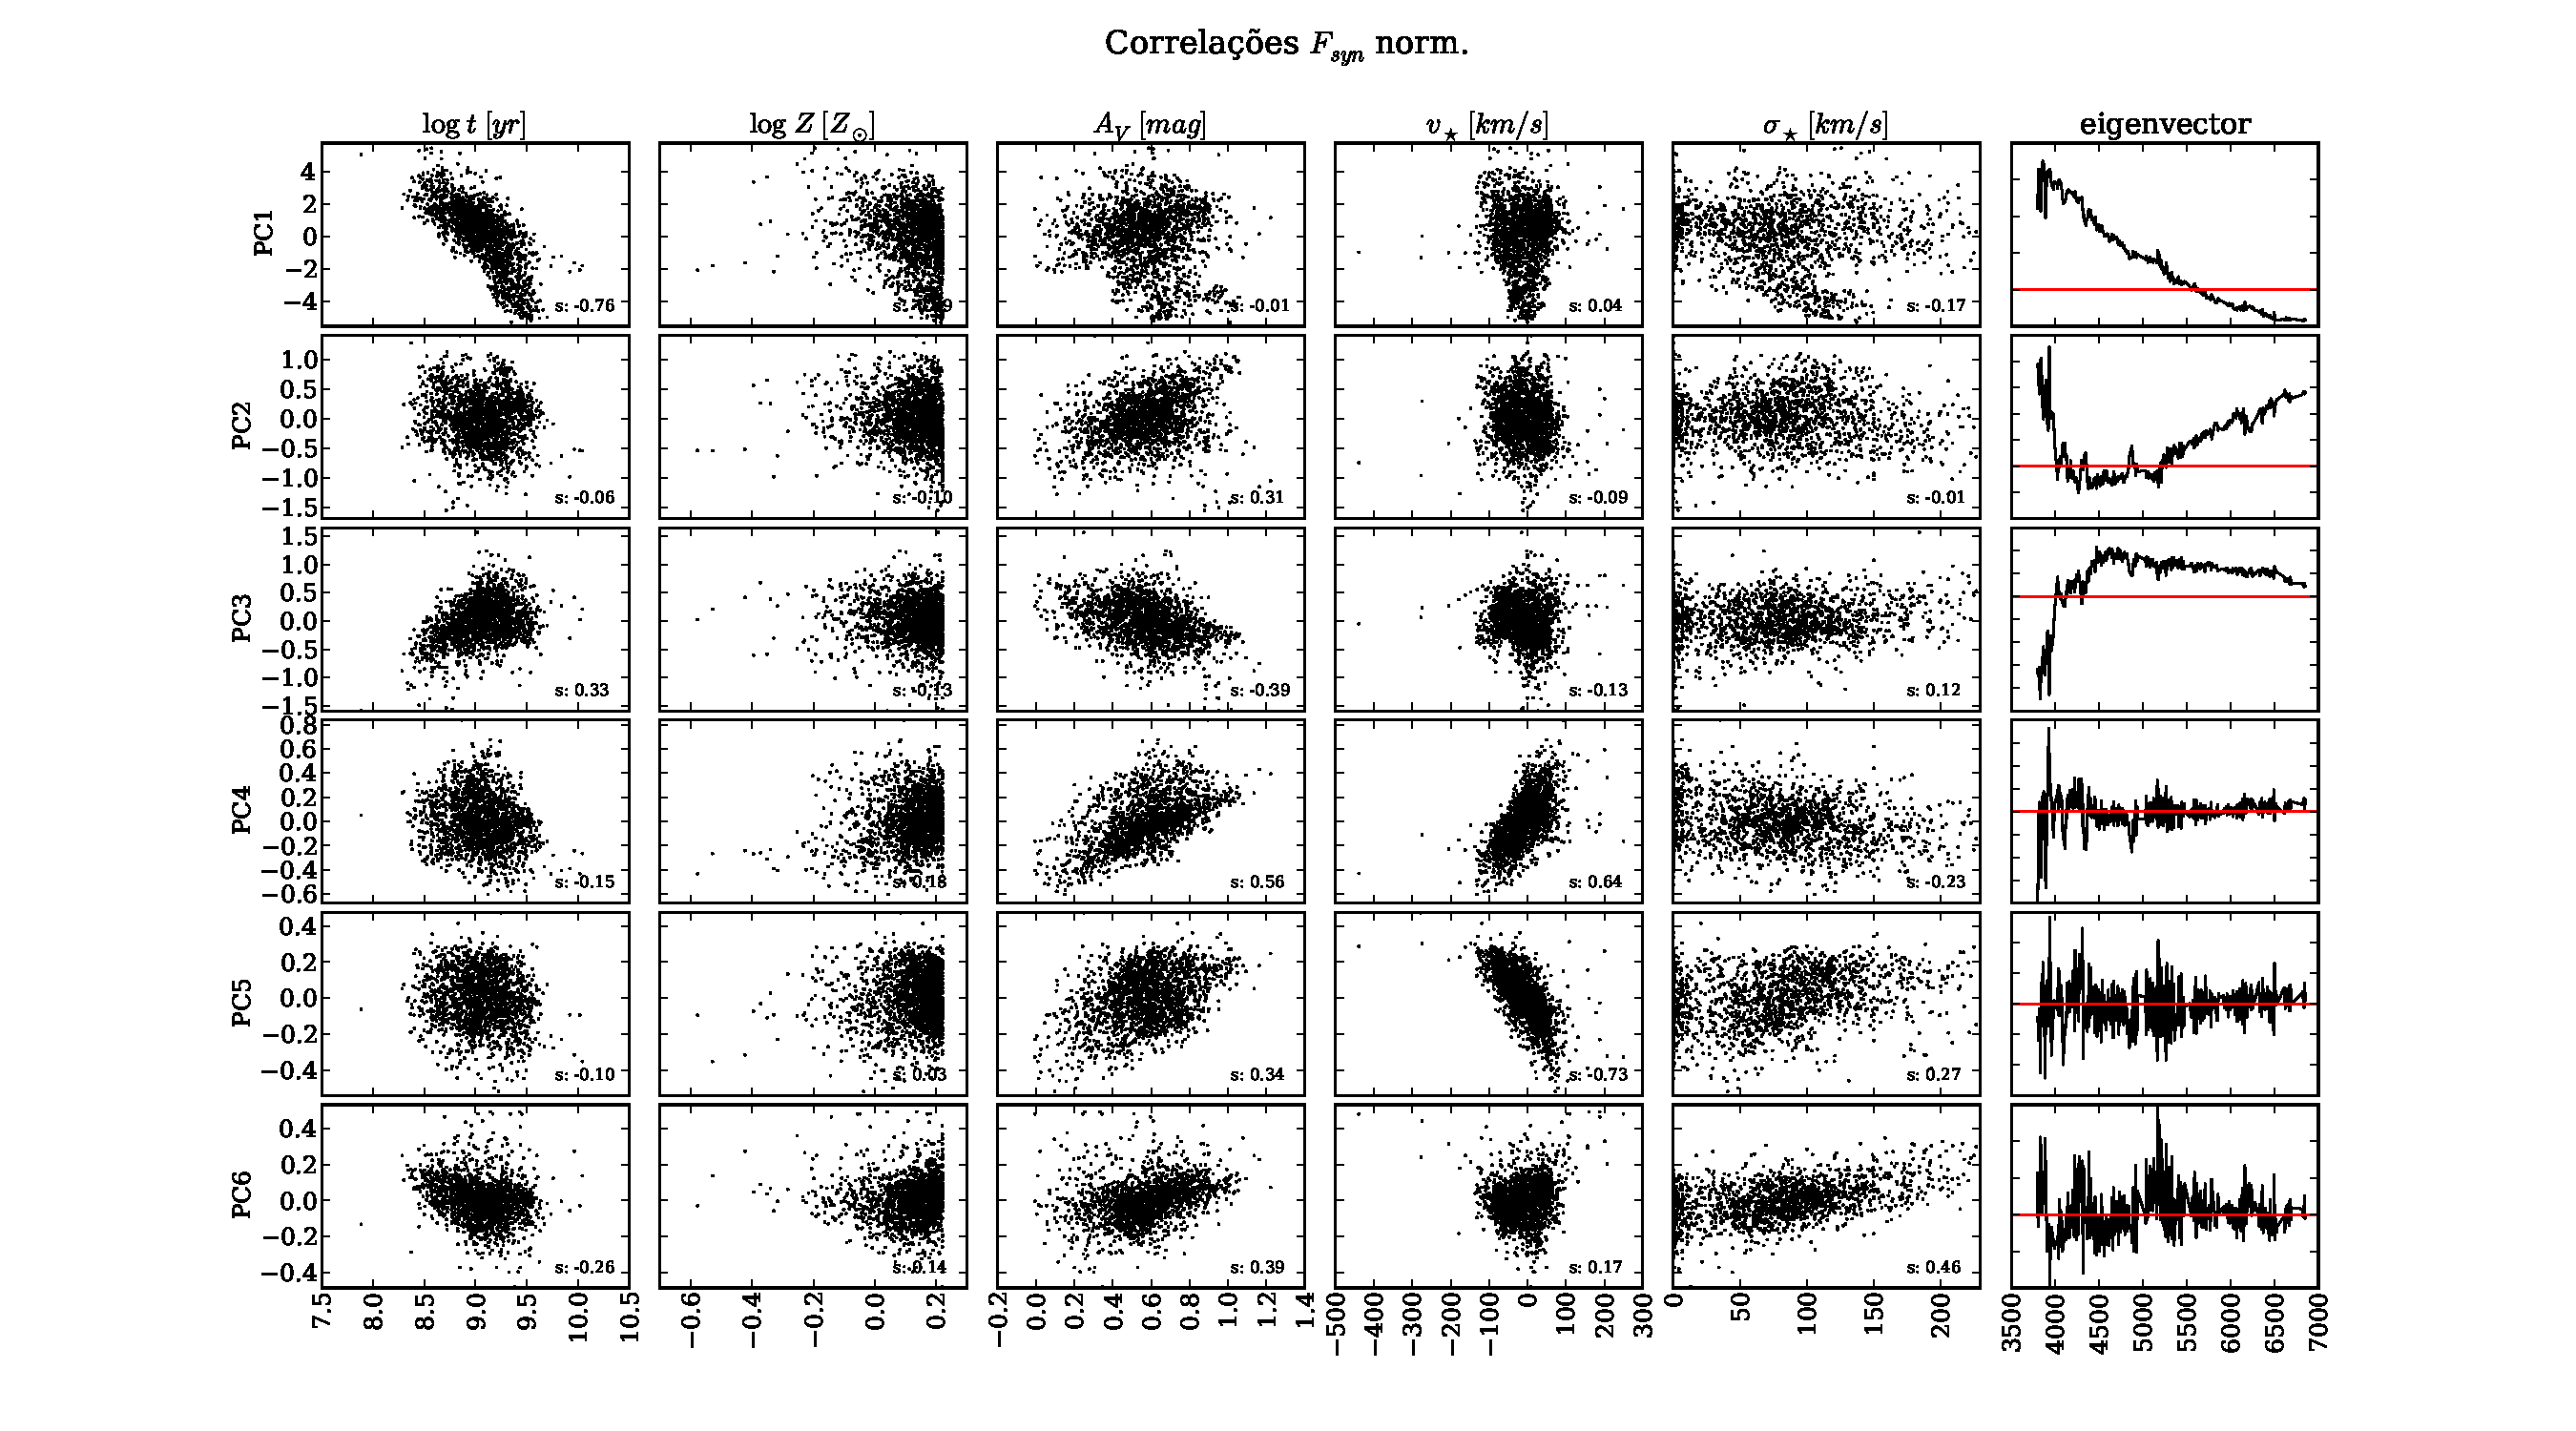
\includegraphics[width=1.2\textwidth, angle=-90]{figuras/K0073-correl-f_syn_norm-PCvsPhys.pdf}
	\caption[Correlações PCs vs. par\^ametros f\'isicos - $f_{syn}$ - NGC 0001]
	{Igual a Figura \ref{fig:K0008correfsynnorm} para a galáxia NGC 0776.}
    \label{fig:K0073correfsynnorm}
\end{figure}

\subsection{NGC 4210 - CALIFA 518}

A galáxia NGC 4210, também é uma espiral com uma barra bem notável, assim como a NGC 0776 (Figura
\ref{fig:K0518apresent}). Pelas figuras podemos notar 3 conjuntos aproximadamente circulares de pixeis à direita do
núcleo. Evidentemente existem problemas com esses pixeis e esses problemas se propagaram para a síntese, fazendo com que
os resultados dessas zonas ficassem díspares ao todo. Esses problemas passaram para o cubo final mesmo passando pelos
{\em pipelines} de redução e os filtros de qualidade do {\sc qbick}. Ao invés de voltar atrás e corrigir esses defeitos,
usaremos esse cubo como exemplo de como o PCA pode nos ajudar a identificar problemas nos dados.

O {\em scree test} (Figura \ref{fig:K0518scree}) apesar de seguir o mesmo padrão das demais parece ter uma distribuição
de variâncias mais parecida entre as PCs para casos diferentes, mas como falamos a seguir, essa galáxia é um caso à
parte.

A tomografia PCA (Figuras \ref{fig:K0518tomofobsnorm} e \ref{fig:K0518tomofsynnorm}) foi capaz de identificar esses
problemas isolando-os nas duas primeiras PCs principalmente, pela extrema variância que eles impõe sobre os espectros.
Na quinta PC para o caso observado vemos também um exemplo de ``linha larga'' ($\sim6000-6200$ \AA) que também foi
causado por defeitos em zonas com espectros defeituosos em nesses comprimentos de onda. Apesar desses problemas, vemos
que para os espectros sintéticos parte deles já desapareceram (veja PC2 em \ref{fig:K0518tomofobsnorm} e compare com a
PC2 em \ref{fig:K0518tomofsynnorm}).

Com esses problemas, o surgimento dessa PC2 no caso observado faz com que fique um pouco mais complicado estudar o
sentido físico dessas PCs, mas olhando as correlações para o caso observado (Figura \ref{fig:K0518correfobsnorm}) vemos
que a PC4 é uma boa medida da velocidade ($s\ =\ 0.80$). Através das correlações usando o resultado para os espectros
sintéticos (Figura \ref{fig:K0518correfsynnorm}) podemos ver que segue o padrão para outras galáxias espirais, onde a
PC1 está geralmente fortemente correlacionada a idade. A PC4, da mesma forma que o observado, reproduz $v_\star$ e a PC5
mais próximo de $A_V$.

\begin{figure}
    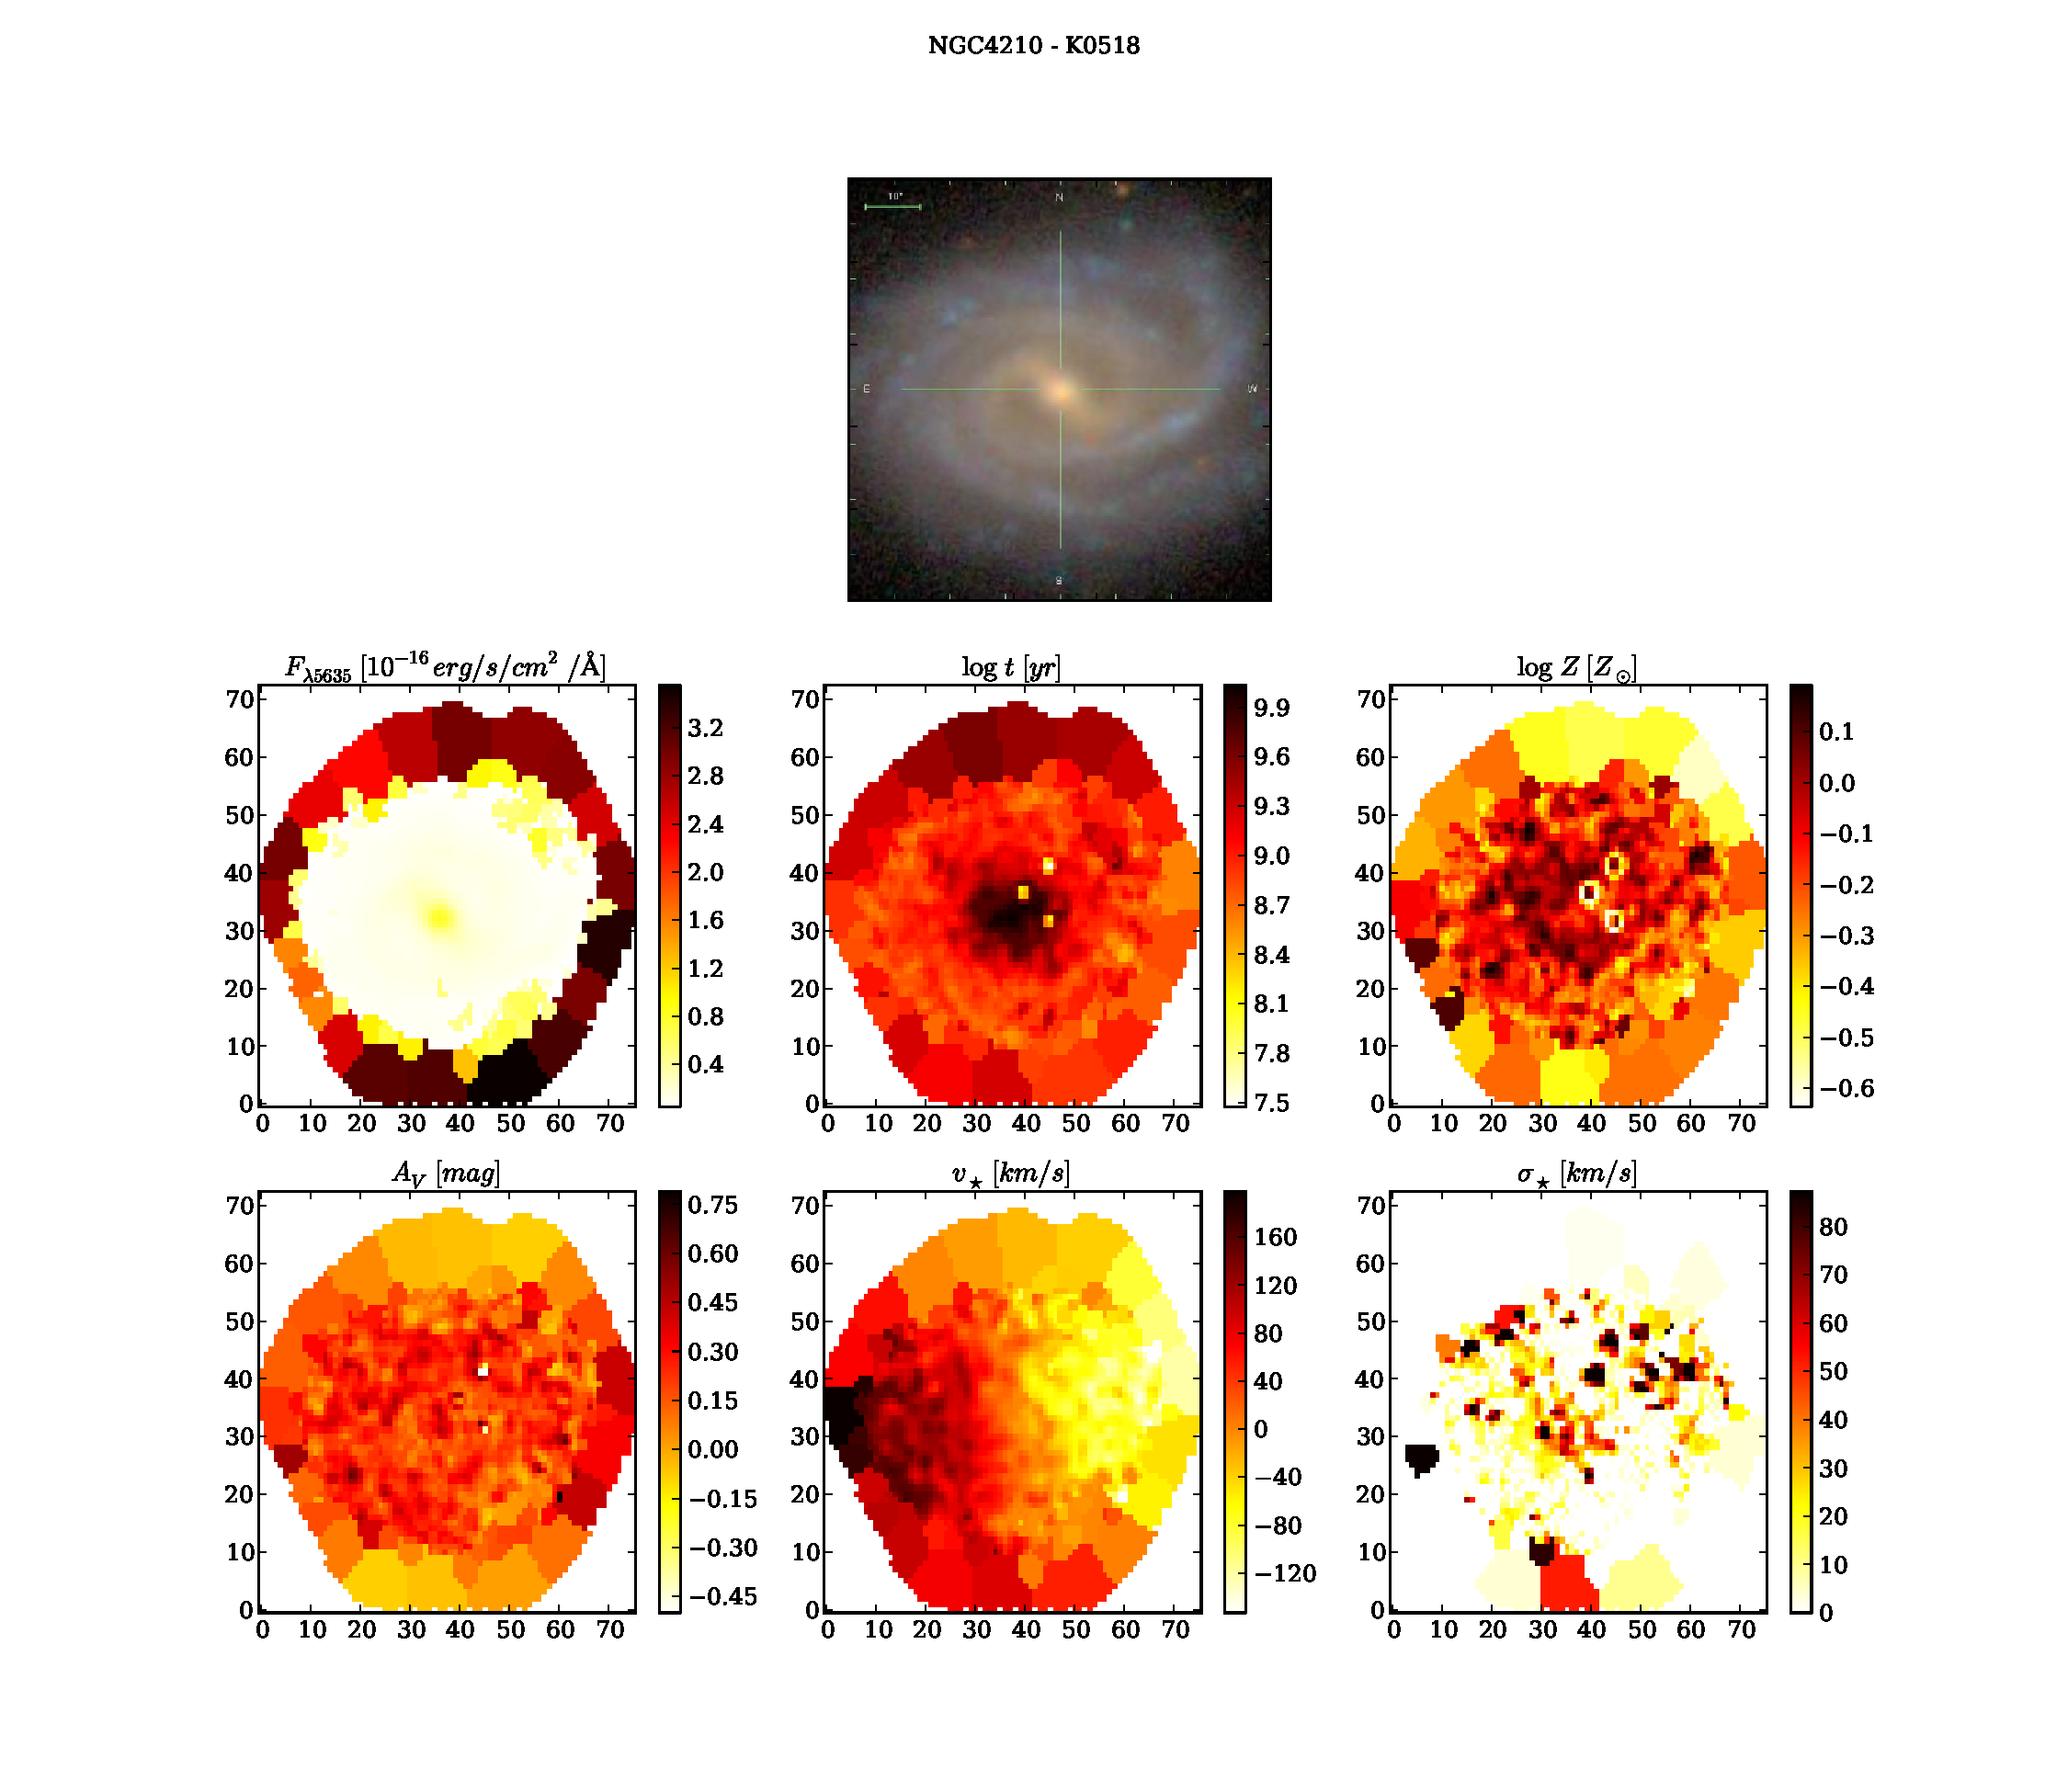
\includegraphics[width=1.\textwidth]{figuras/K0518-apresent.pdf}
    \caption[Propriedades f\'isicas da gal\'axia NGC 4210.]
    {Igual a Figura \ref{fig:K0008apresent} para a galáxia NGC 4210.}
    \label{fig:K0518apresent}
\end{figure}

\begin{figure}
    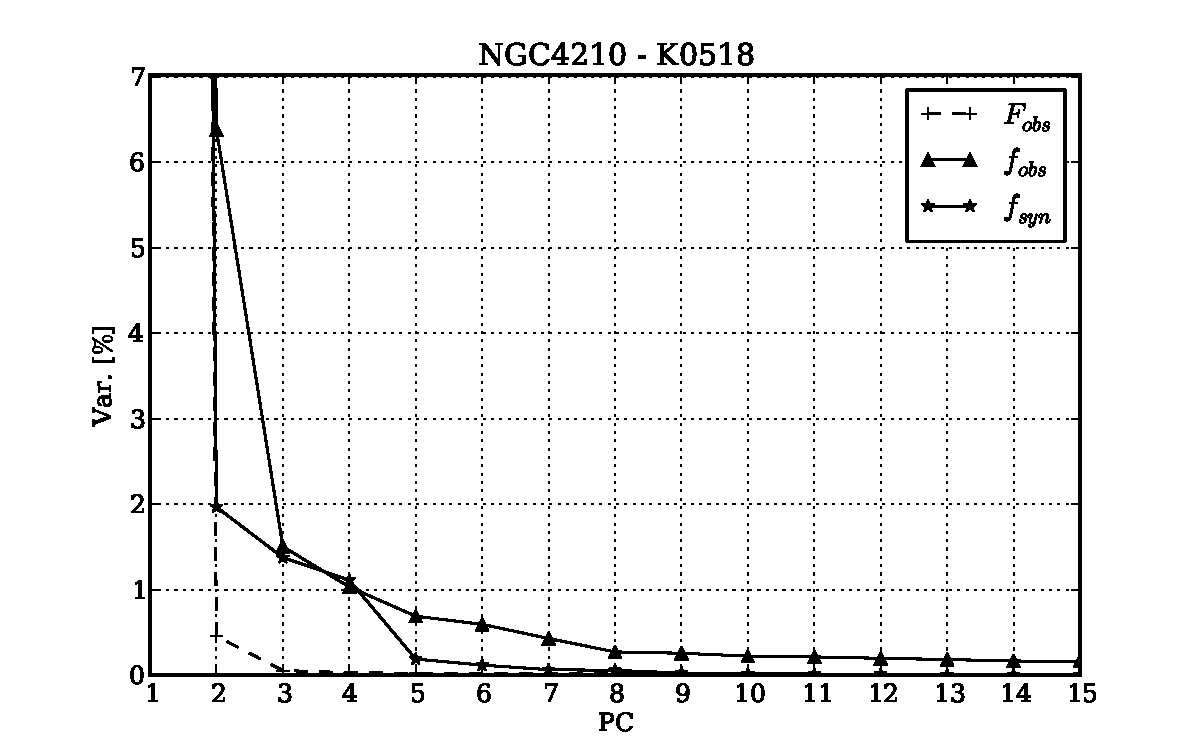
\includegraphics[height=0.33\textheight]{figuras/K0518-screetest.pdf}
    \caption[Scree test comparativo entre 3 PCAs - NGC 4210.]
	{Igual a Figura \ref{fig:K0008scree} para a galáxia NGC 4210.}
    \label{fig:K0518scree}
\end{figure}

\begin{figure}
    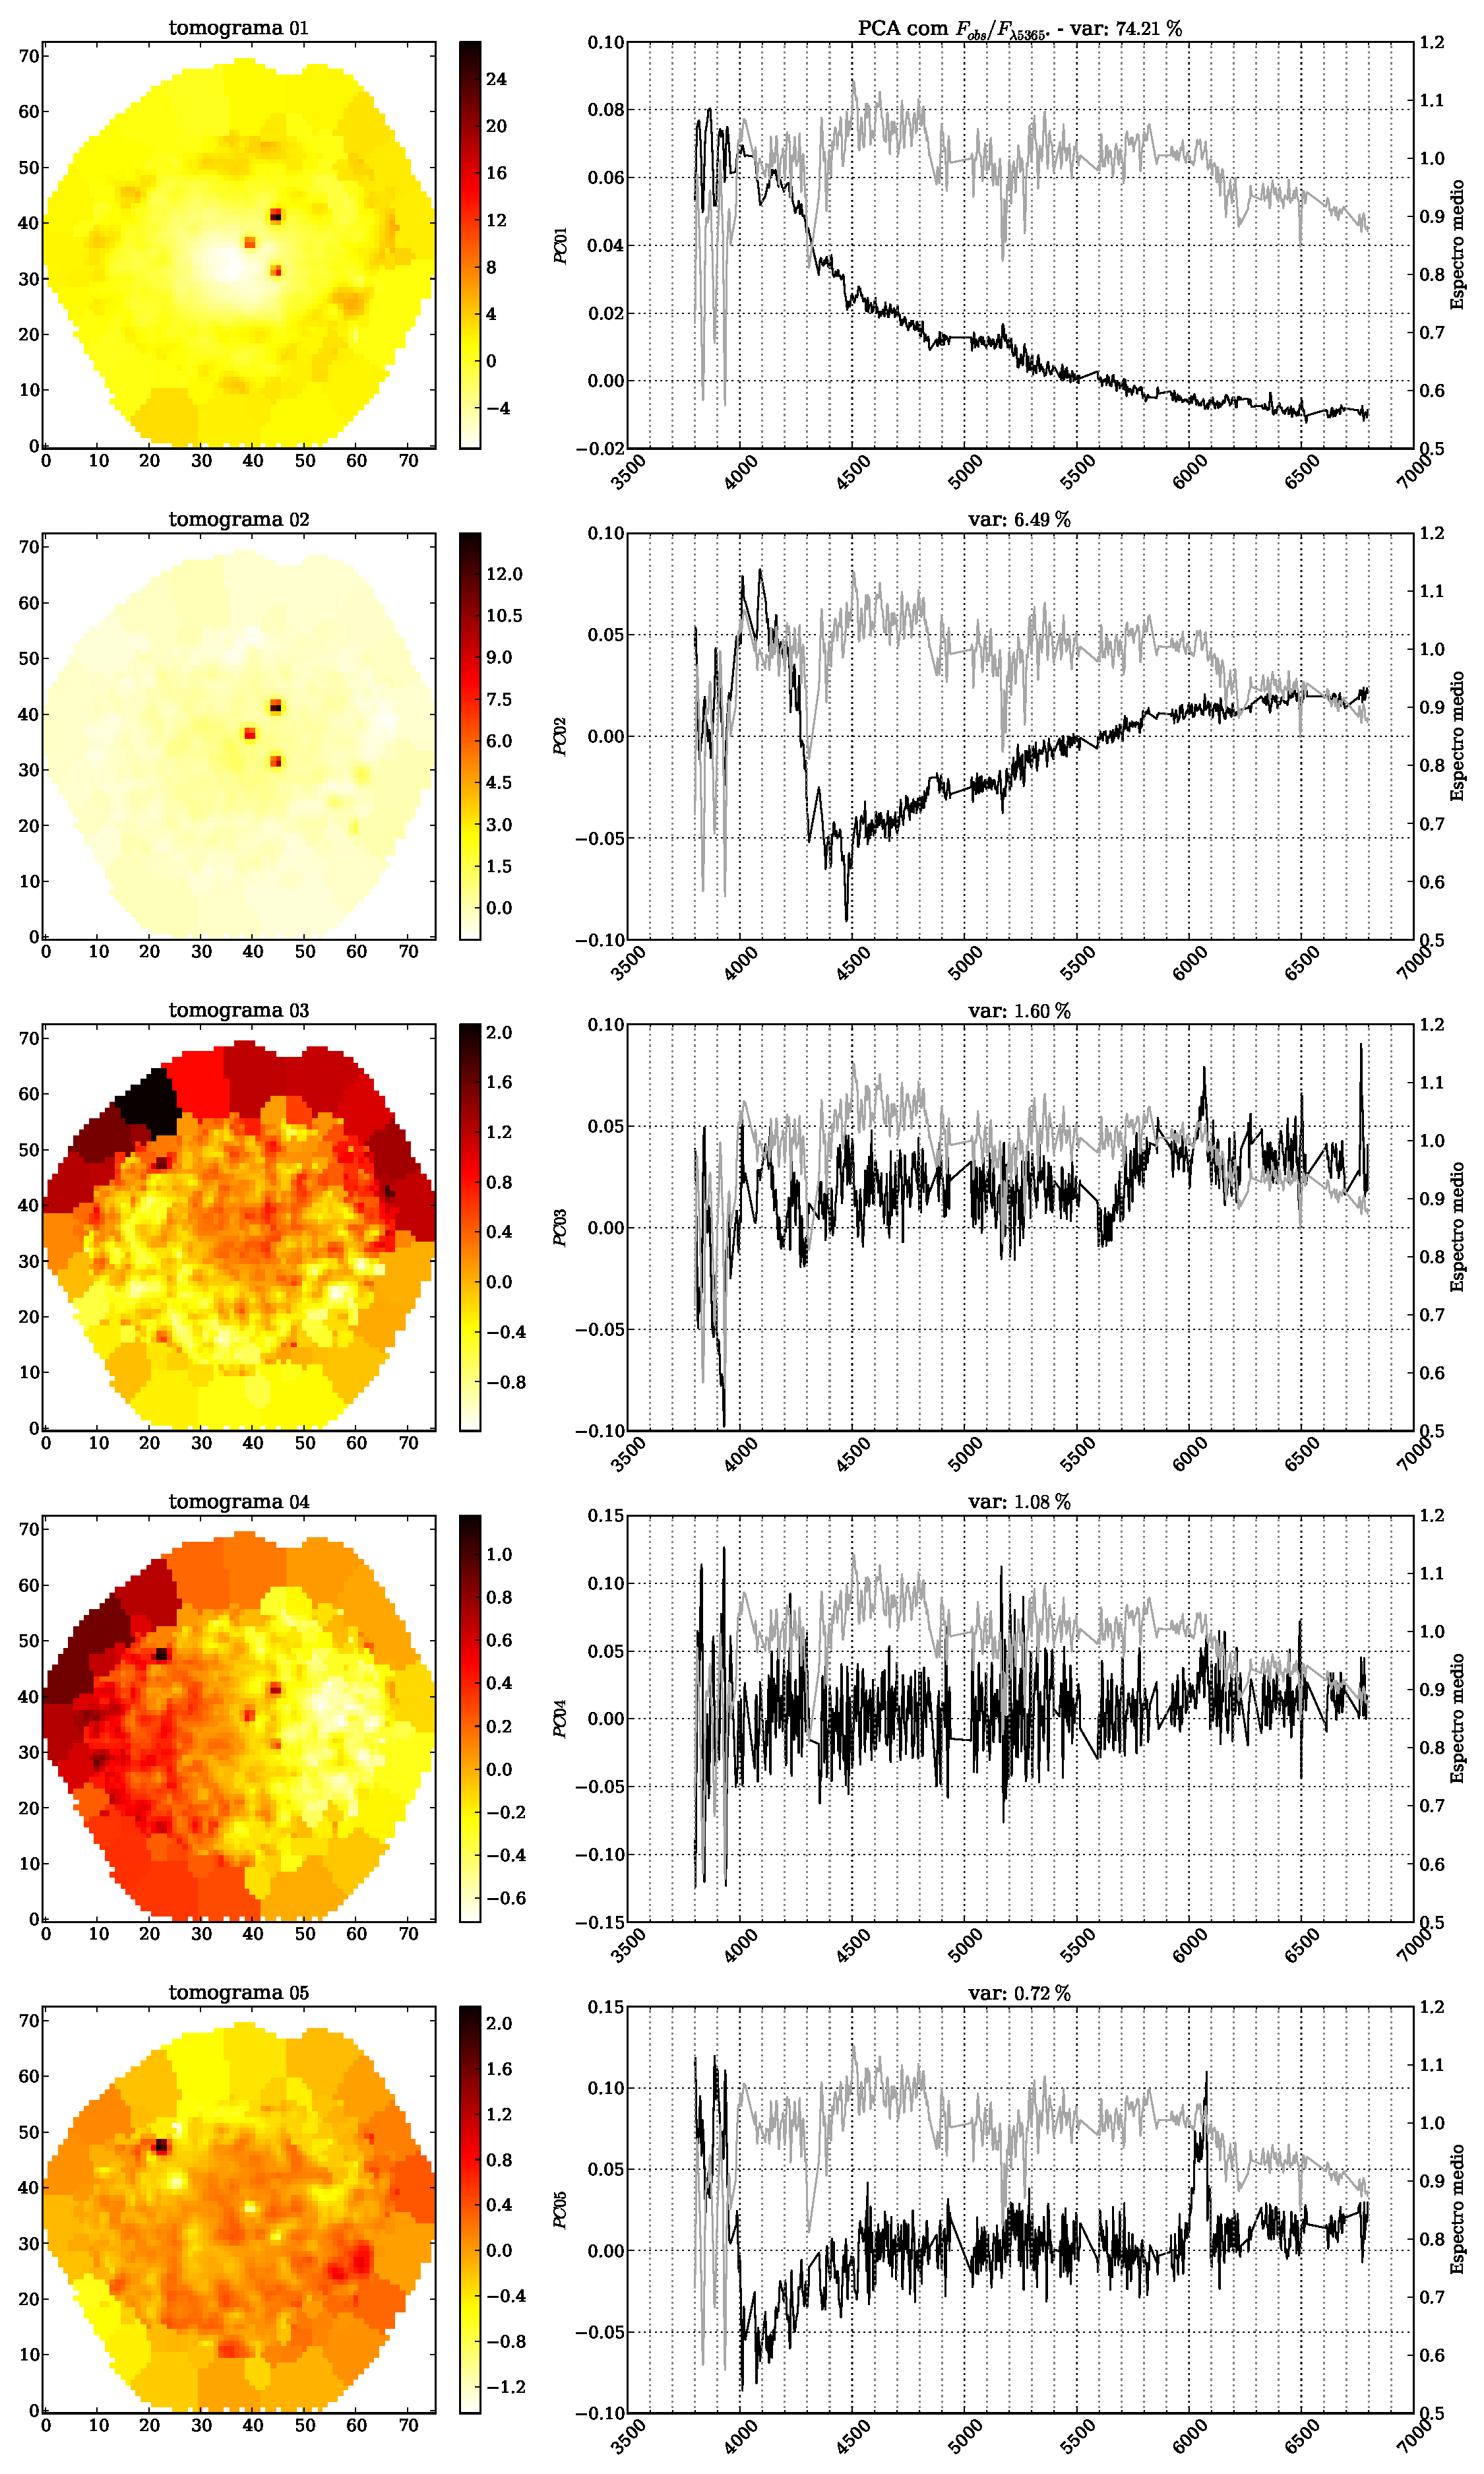
\includegraphics[width=0.8\textwidth]{figuras/K0518-tomo-obs-norm.pdf}
    \caption[Tomogramas de 1 a 5 para o cubo $f_{obs}$ - NGC 4210.]
    {Igual a Figura \ref{fig:K0008tomofobsnorm} para a galáxia NGC 4210.}
    \label{fig:K0518tomofobsnorm}
\end{figure}

\begin{figure}
    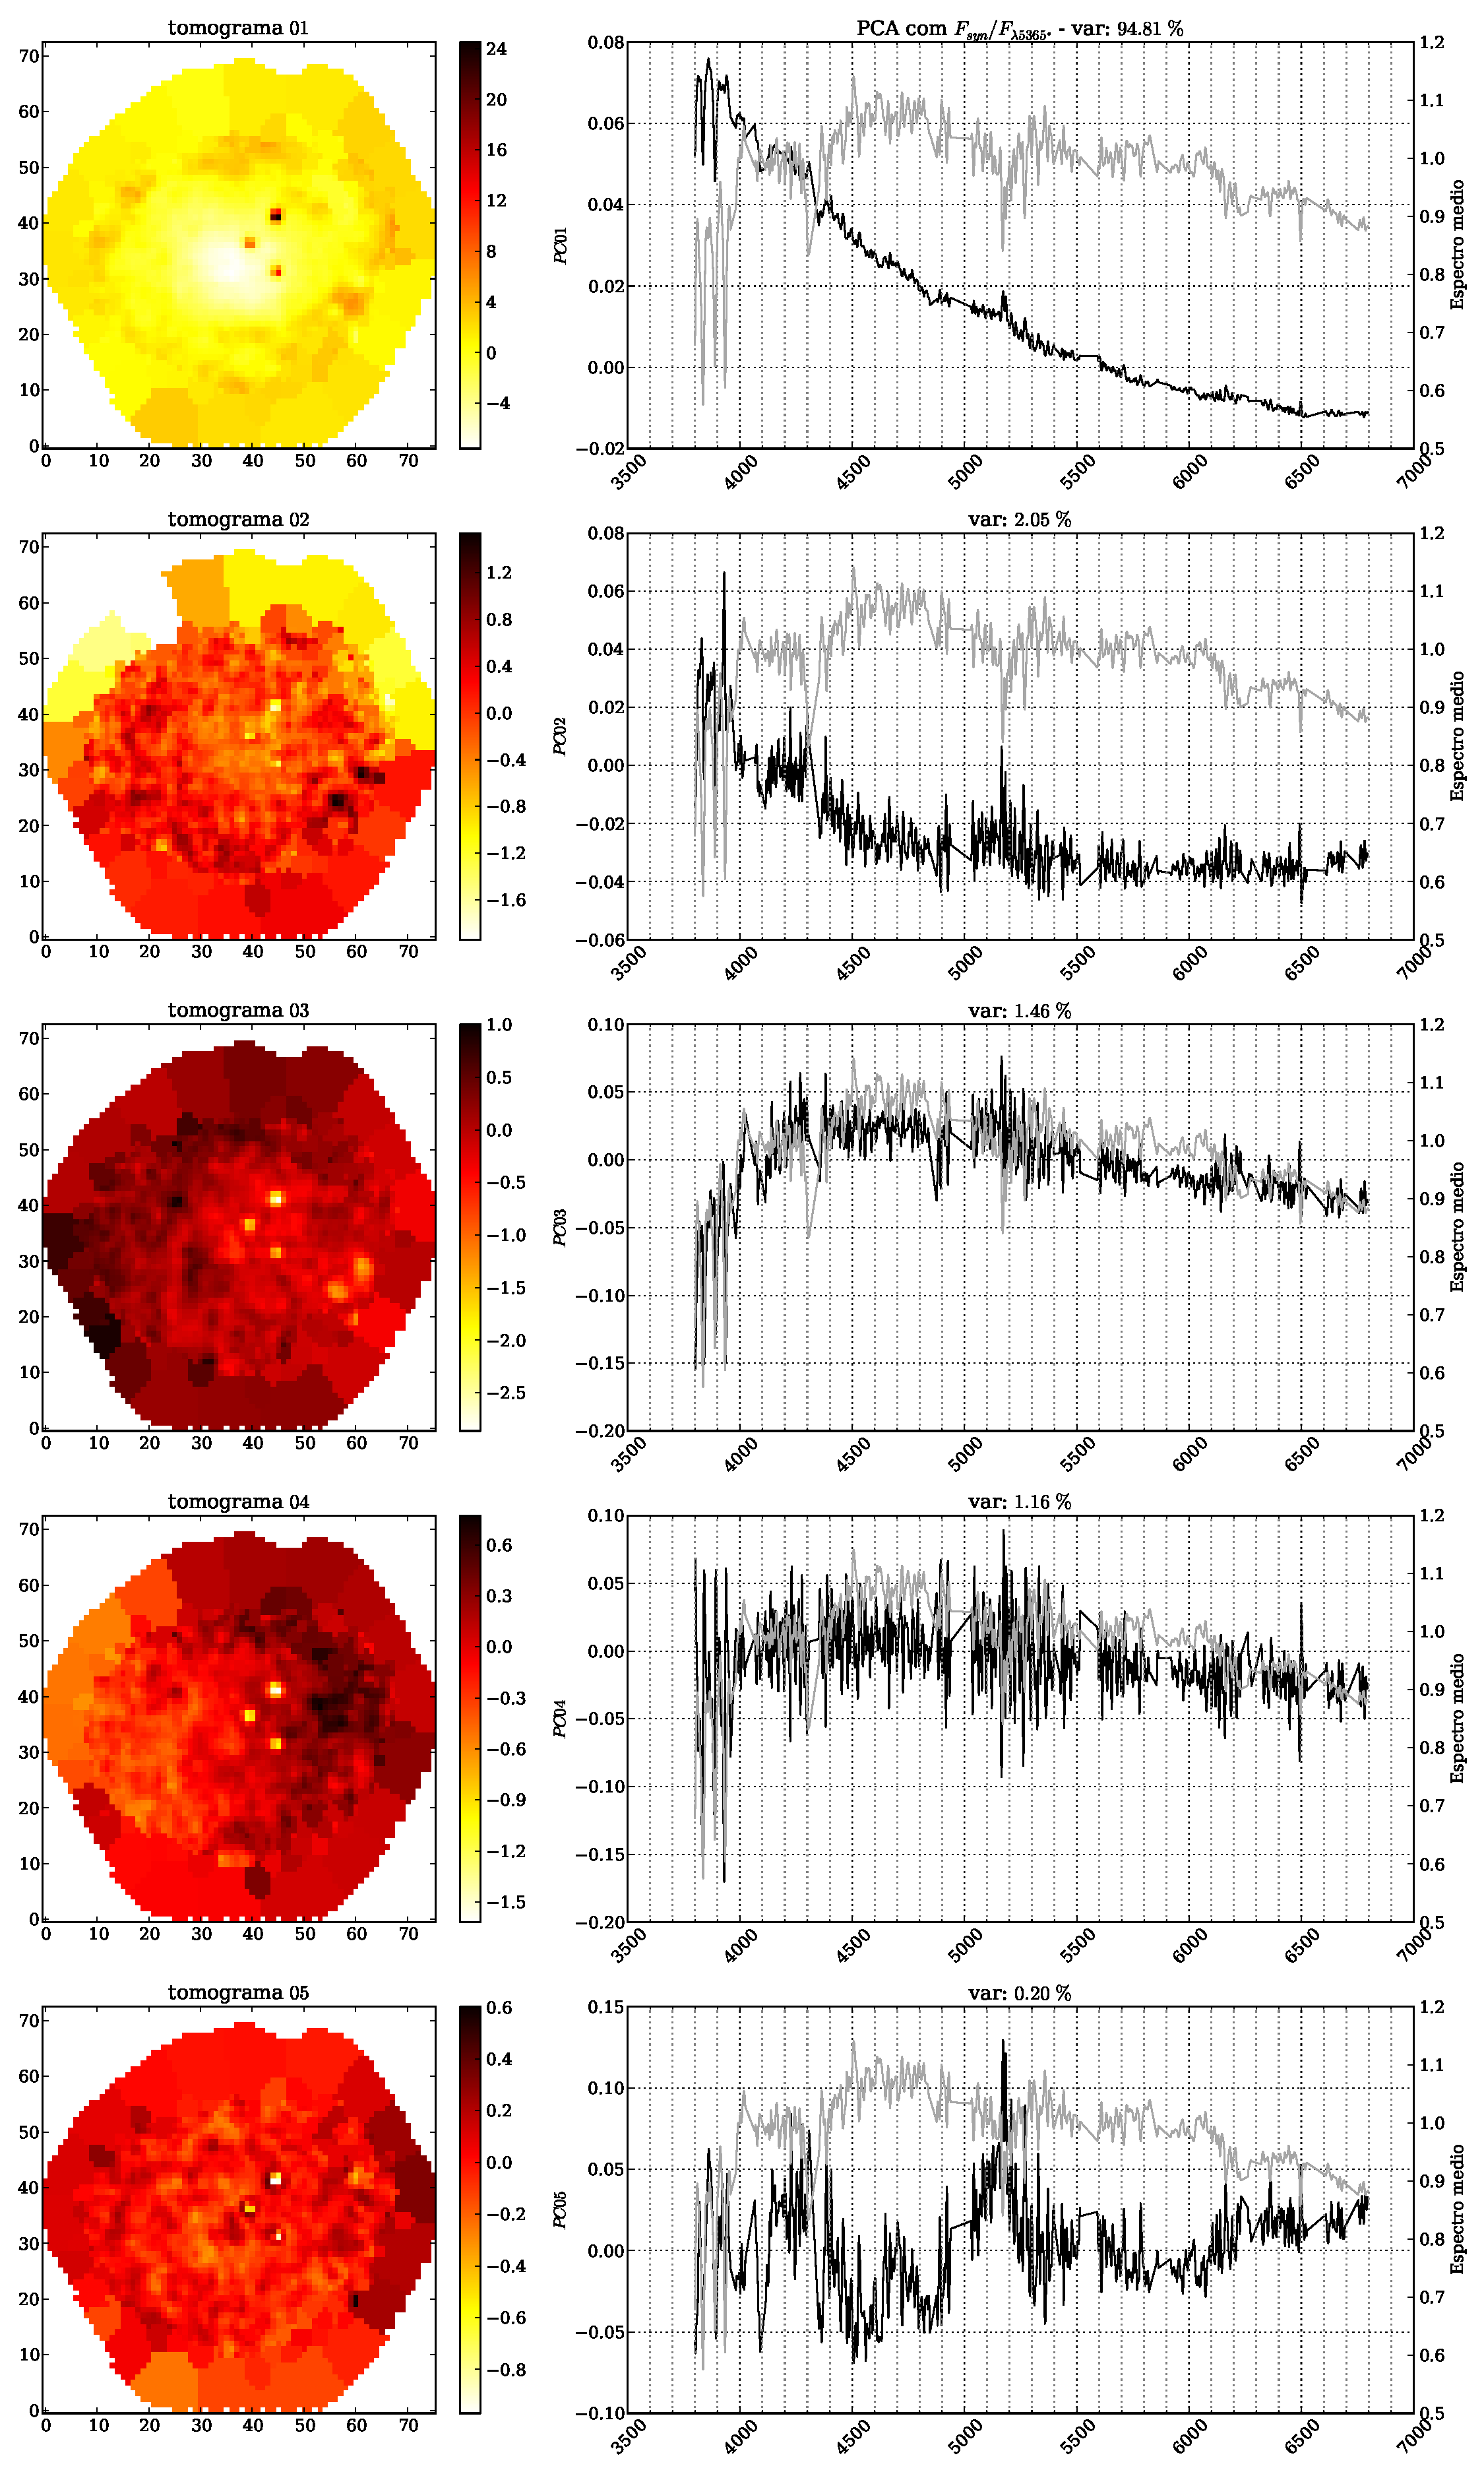
\includegraphics[width=0.8\textwidth]{figuras/K0518-tomo-syn-norm.pdf}
    \caption[Tomogramas de 1 a 5 para o cubo $f_{syn}$ - NGC 4210.]
    {Igual a Figura \ref{fig:K0008tomofsynnorm} para a galáxia NGC 4210.}
    \label{fig:K0518tomofsynnorm}
\end{figure}

\begin{figure}
    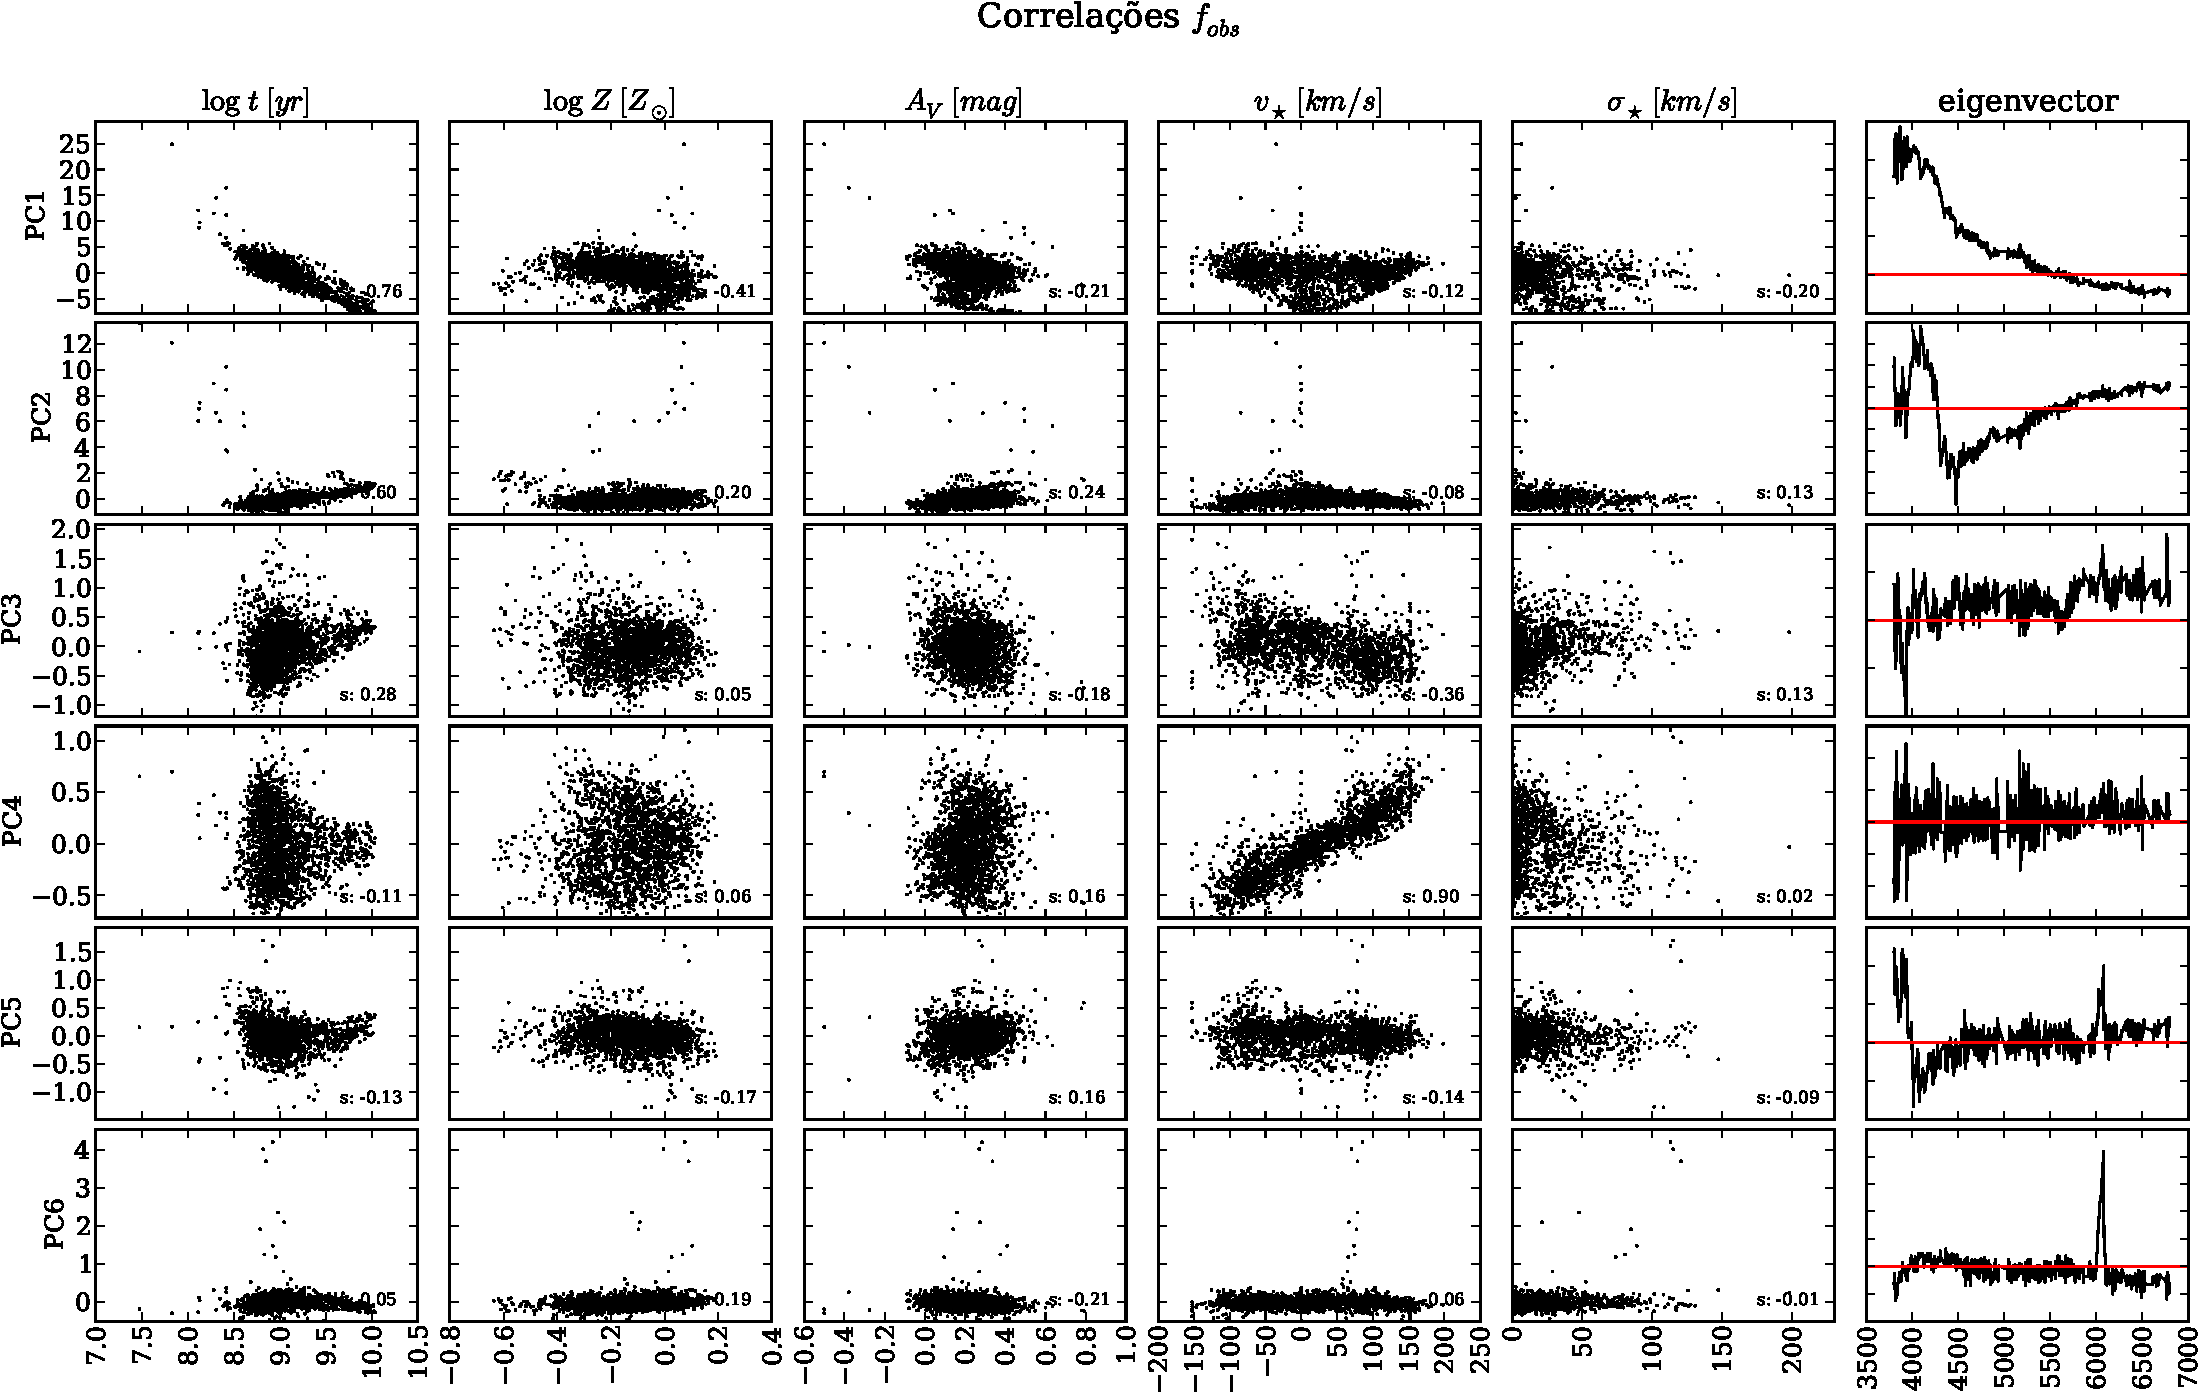
\includegraphics[width=1.2\textwidth, angle=-90]{figuras/K0518-correl-f_obs_norm-PCvsPhys.pdf}
	\caption[Correlações PCs vs. par\^ametros f\'isicos - $f_{obs}$ - NGC 4210.]
	{Igual a Figura \ref{fig:K0008correfobsnorm} para a galáxia NGC 4210.}
    \label{fig:K0518correfobsnorm}
\end{figure}

\begin{figure}
    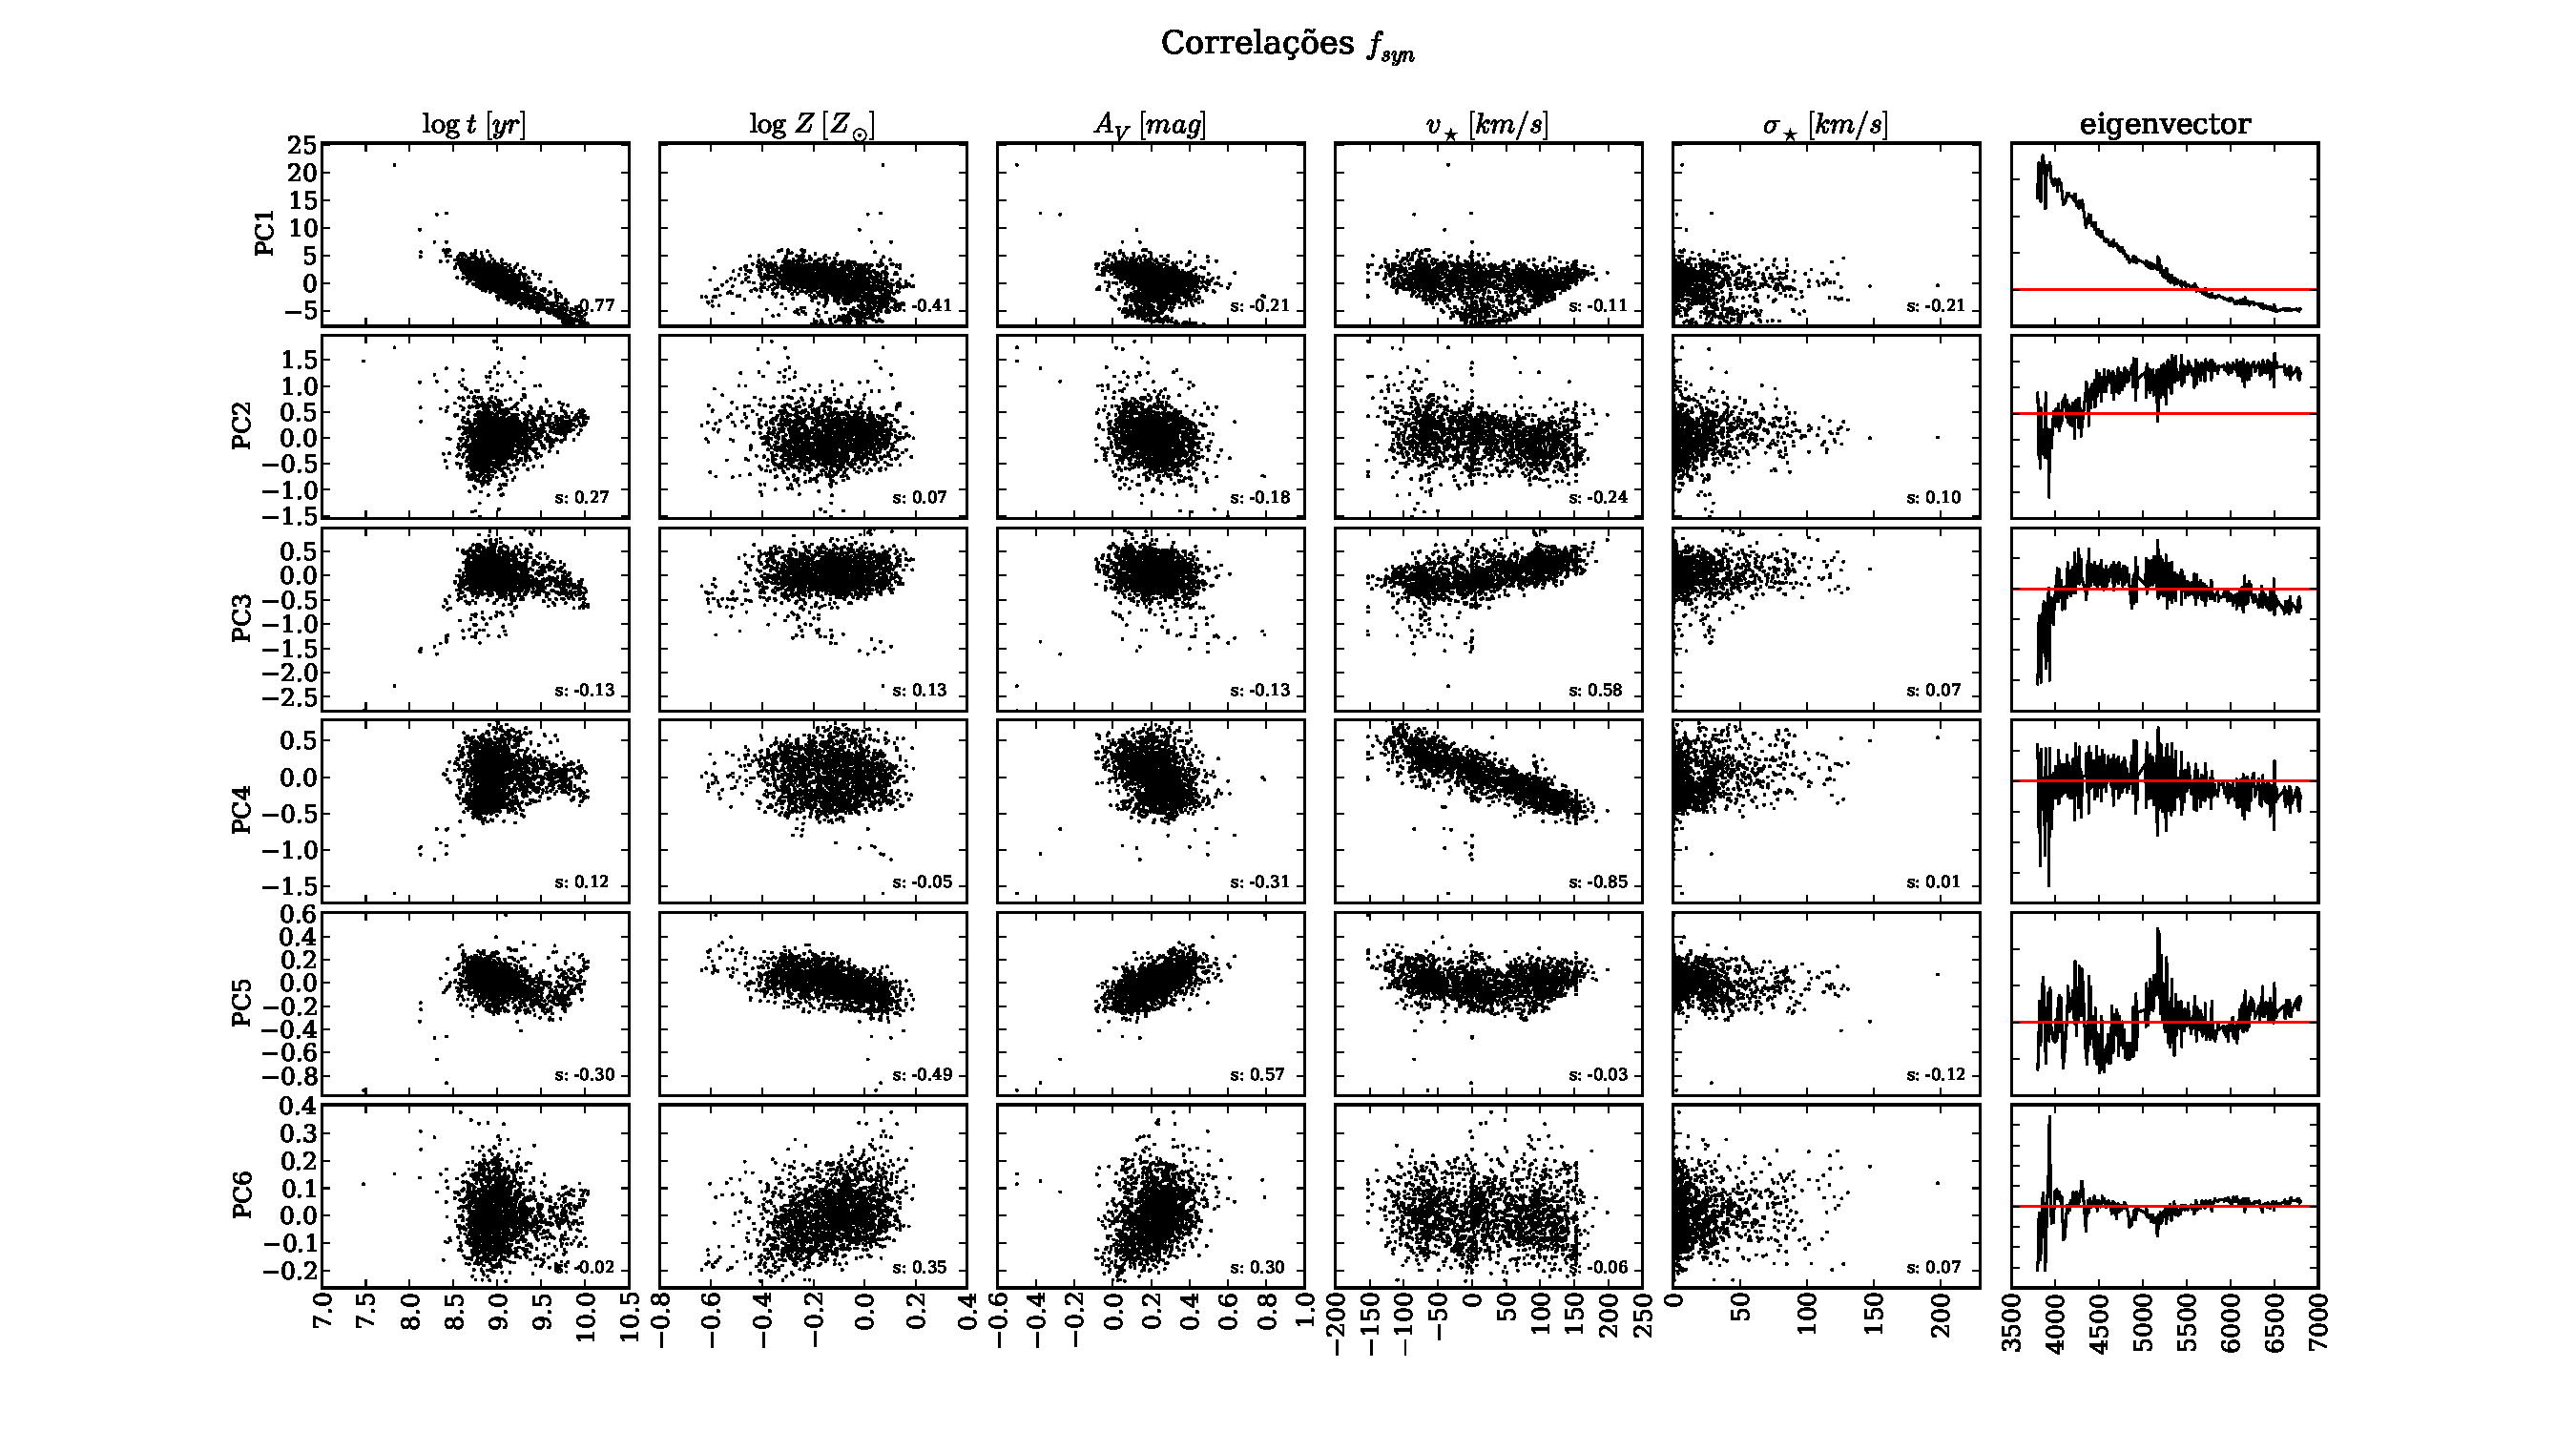
\includegraphics[width=1.2\textwidth, angle=-90]{figuras/K0518-correl-f_syn_norm-PCvsPhys.pdf}
	\caption[Correlações PCs vs. par\^ametros f\'isicos -um padrão de velocidades $f_{syn}$ - NGC 4210.]
	{Igual a Figura \ref{fig:K0008correfsynnorm} para a galáxia NGC 4210.}
    \label{fig:K0518correfsynnorm}
\end{figure}

\section{Gal\'axias {\em early-type}}
\label{sec:result:elipt}

Galáxias elípticas e S0 são sabidamente mais simples do que espirais, tanto em termos de estruturas morfológicas como em
suas populacoes estelares, mais velhas do que aquelas encontradas nos discos (e as vezes nas regiões centrais) de
espirais. Elas também contêm menos poeira, sendo essa também distribuída de forma mais regular. Esta maior homogeneidade
das propriedades dessas galáxias sugere uma menor variância espectral. Vejamos o que a tomografia PCA revela em duas
galáxias early type.

\subsection{NGC 1167 - CALIFA 119}

Pela apresentação das propriedades físicas dessa galáxia (Figura \ref{fig:K0119apresent}), cores na imagem SDSS,
distribuição de idades, e grande dispersão de velocidades no centro, já mostram o quanto essa galáxia é diferente de
todas que exploramos até agora.

No {\em scree test} o comportamento assintótico é o mesmo para as outras galáxias, com a variância mais distribuída
entre as primeiras PCs no caso sintético. A segunda componente do caso sintético nem aparece no gráfico, mas pelo seu
tomograma (Figura \ref{fig:K0119tomofsynnorm}) vemos que ela possui $\sim 35\%$ da variância.

Vemos que a PC1 dos dois casos (Figuras \ref{fig:K0119tomofobsnorm} e \ref{fig:K0119tomofsynnorm}) são bem diferentes e
no caso sintético ela não é correlacionada com alguma propriedade específica. Já no caso observado ela exibe uma ótima
correlação com $A_V$ e com a metalicidade. No sintético $A_V$ aparece principalmente na PC2, também misturada com a
metalicidade. A PC5 do caso observado também correlaciona bem com $A_V$. O padrão de velocidades aparece de forma muito
clara para ambos os casos na PC3, com um incrível índice de correlação de Spearman de 0.98 para o caso sintético. Vemos
que a dispersão de velocidades ($\sigma_\star$) aparece correlacionando fracamente com quase todas as principais PCs,
mas no caso sintético vemos uma correlação maior ($s\ =\ 0.53$). A idade média estelar fica mais distribuída entre as
PC5 e PC6 no caso sintético, mas mesmo assim com correlações não tão gritantes quanto para as galáxias espirais. Já no
caso observado correlaciona um pouco com a PC2 mas nada muito evidente também.

\begin{figure}
    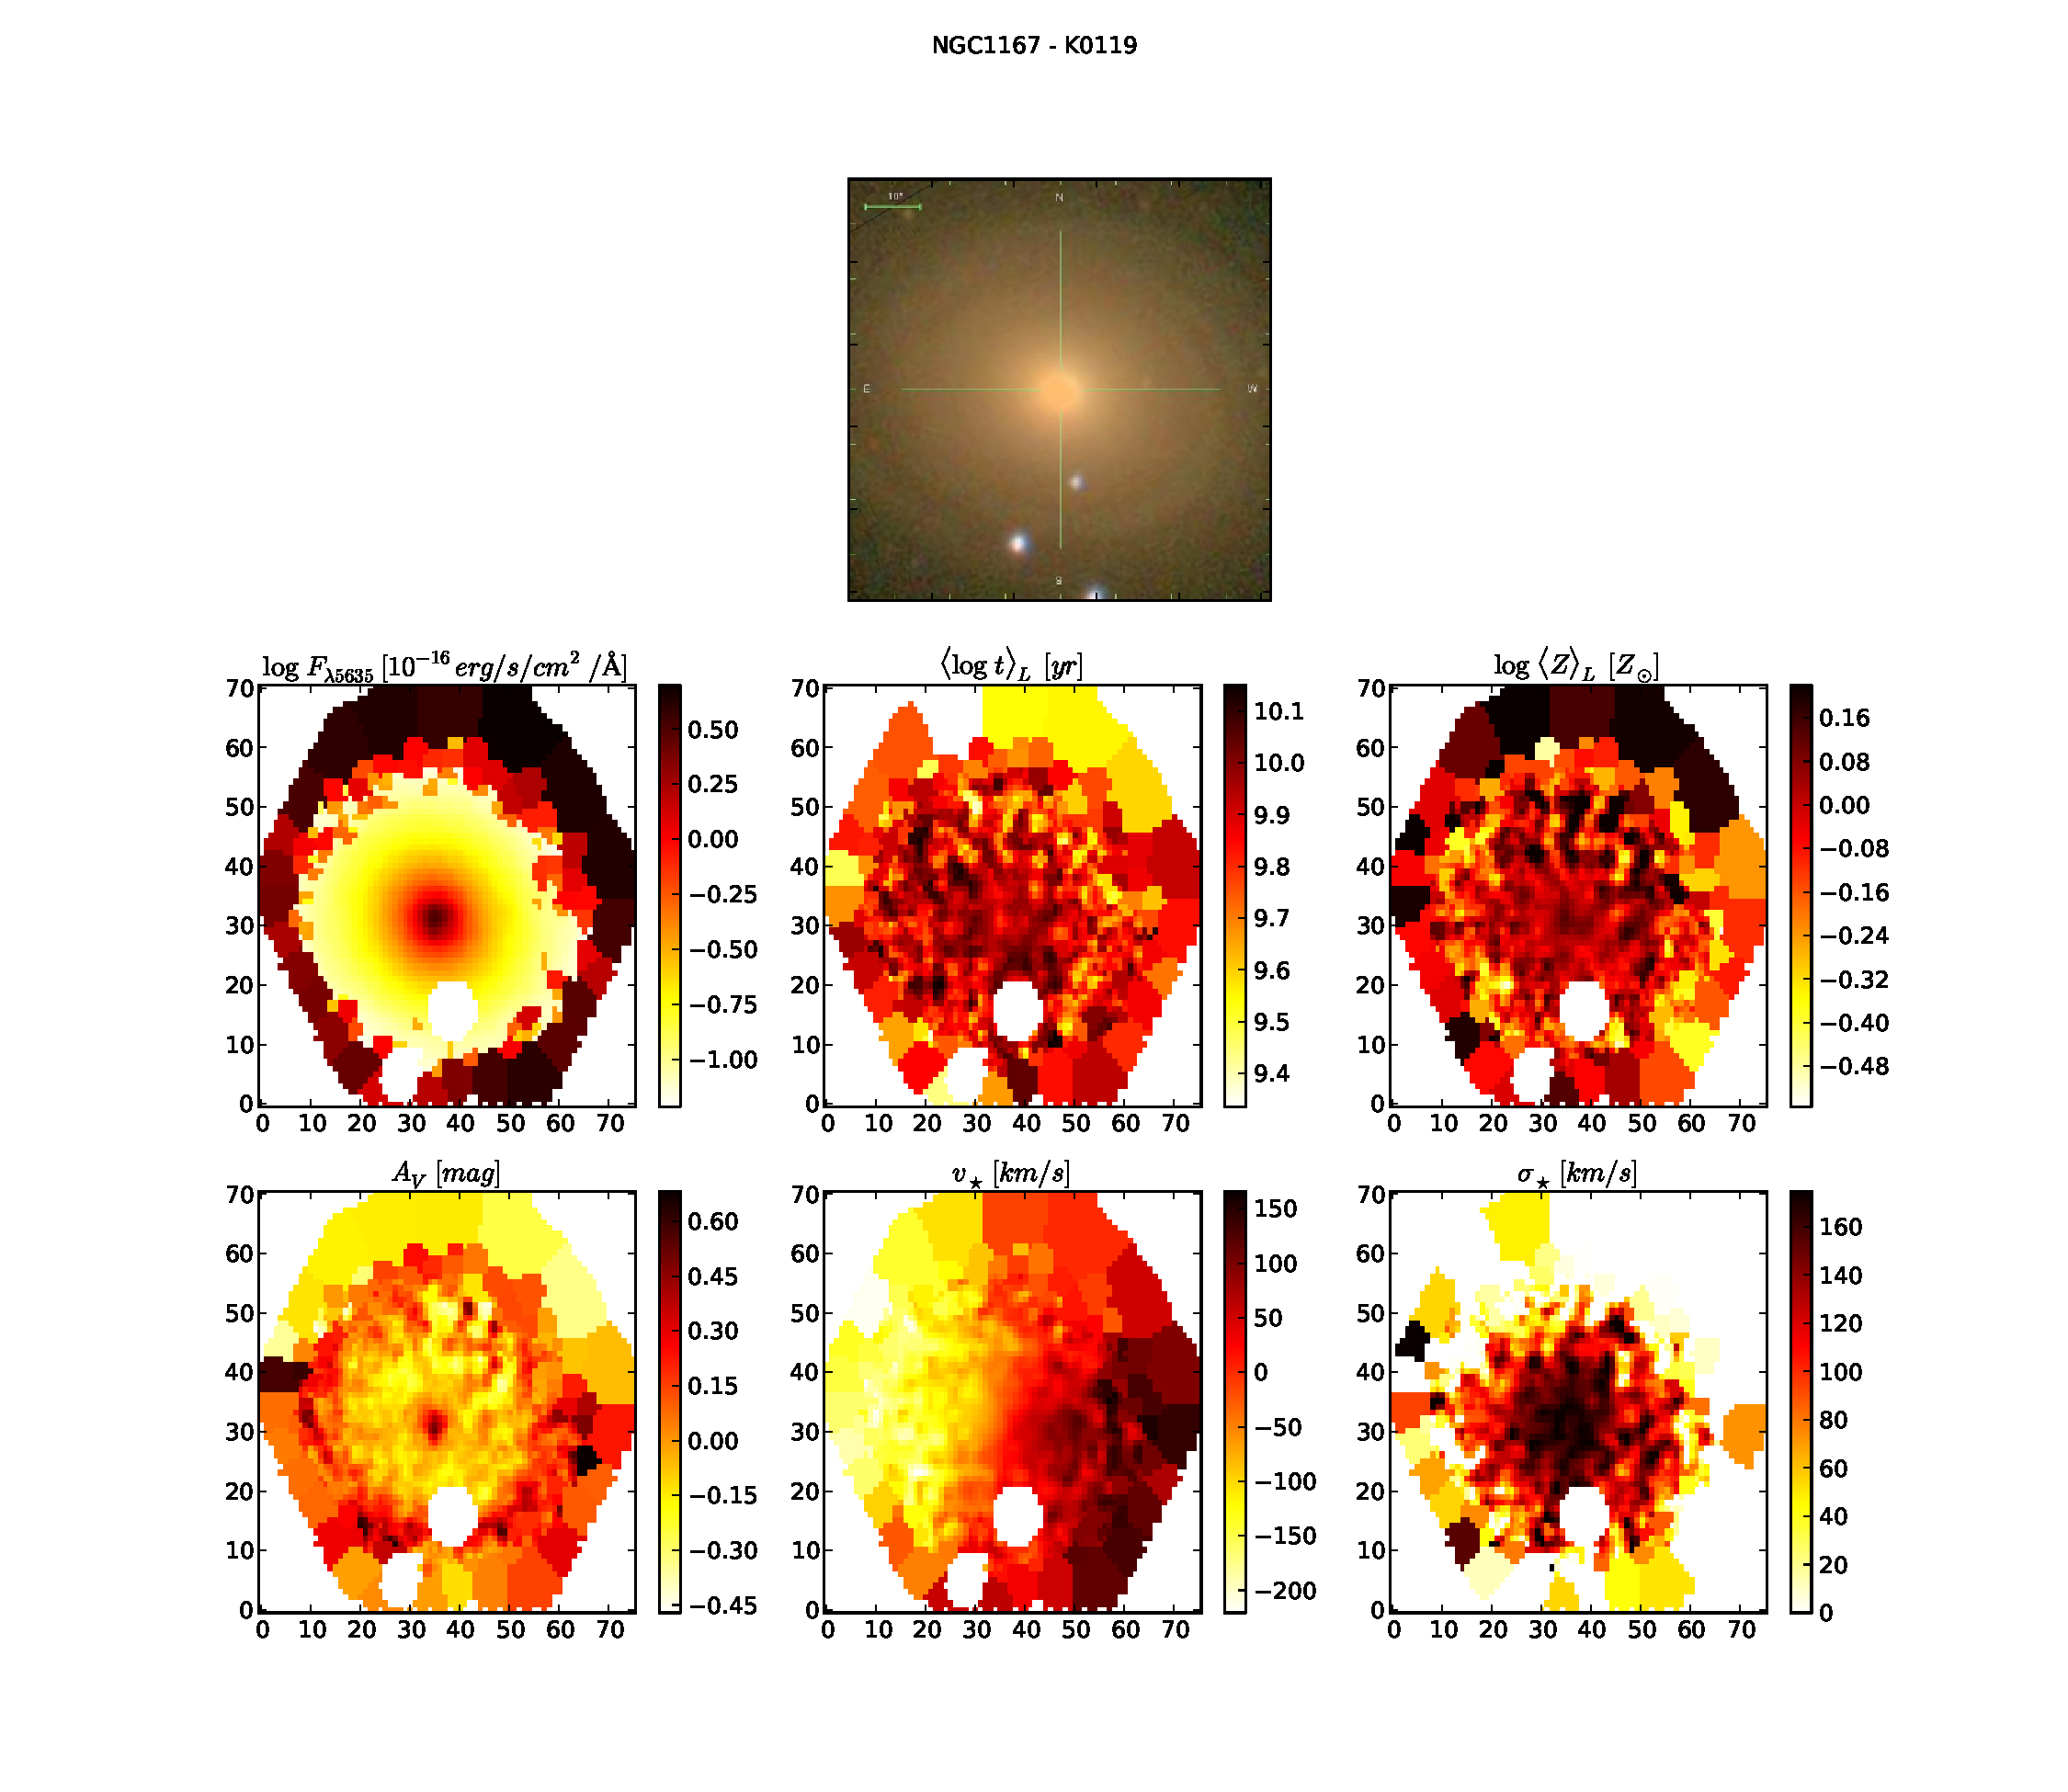
\includegraphics[width=1.\textwidth]{figuras/K0119-apresent.pdf}
    \caption[Propriedades f\'isicas da gal\'axia NGC 1167.]
    {Igual a Figura \ref{fig:K0008apresent} para a galáxia NGC 1167.}
    \label{fig:K0119apresent}
\end{figure}

\begin{figure}
    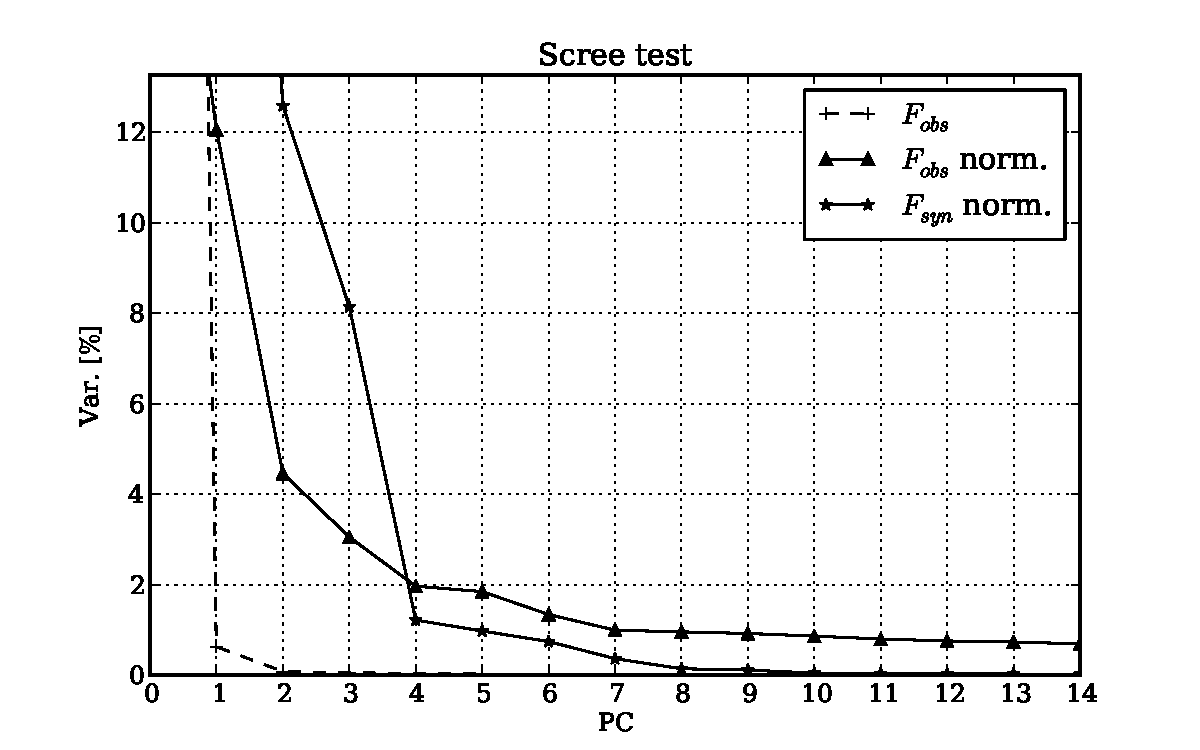
\includegraphics[height=0.33\textheight]{figuras/K0119-screetest.pdf}
    \caption[Scree test comparativo entre 3 PCAs - NGC 1167.]
    {Igual a Figura \ref{fig:K0008scree} para a galáxia NGC 1167.}
    \label{fig:K0119scree}
\end{figure}

\begin{figure}
    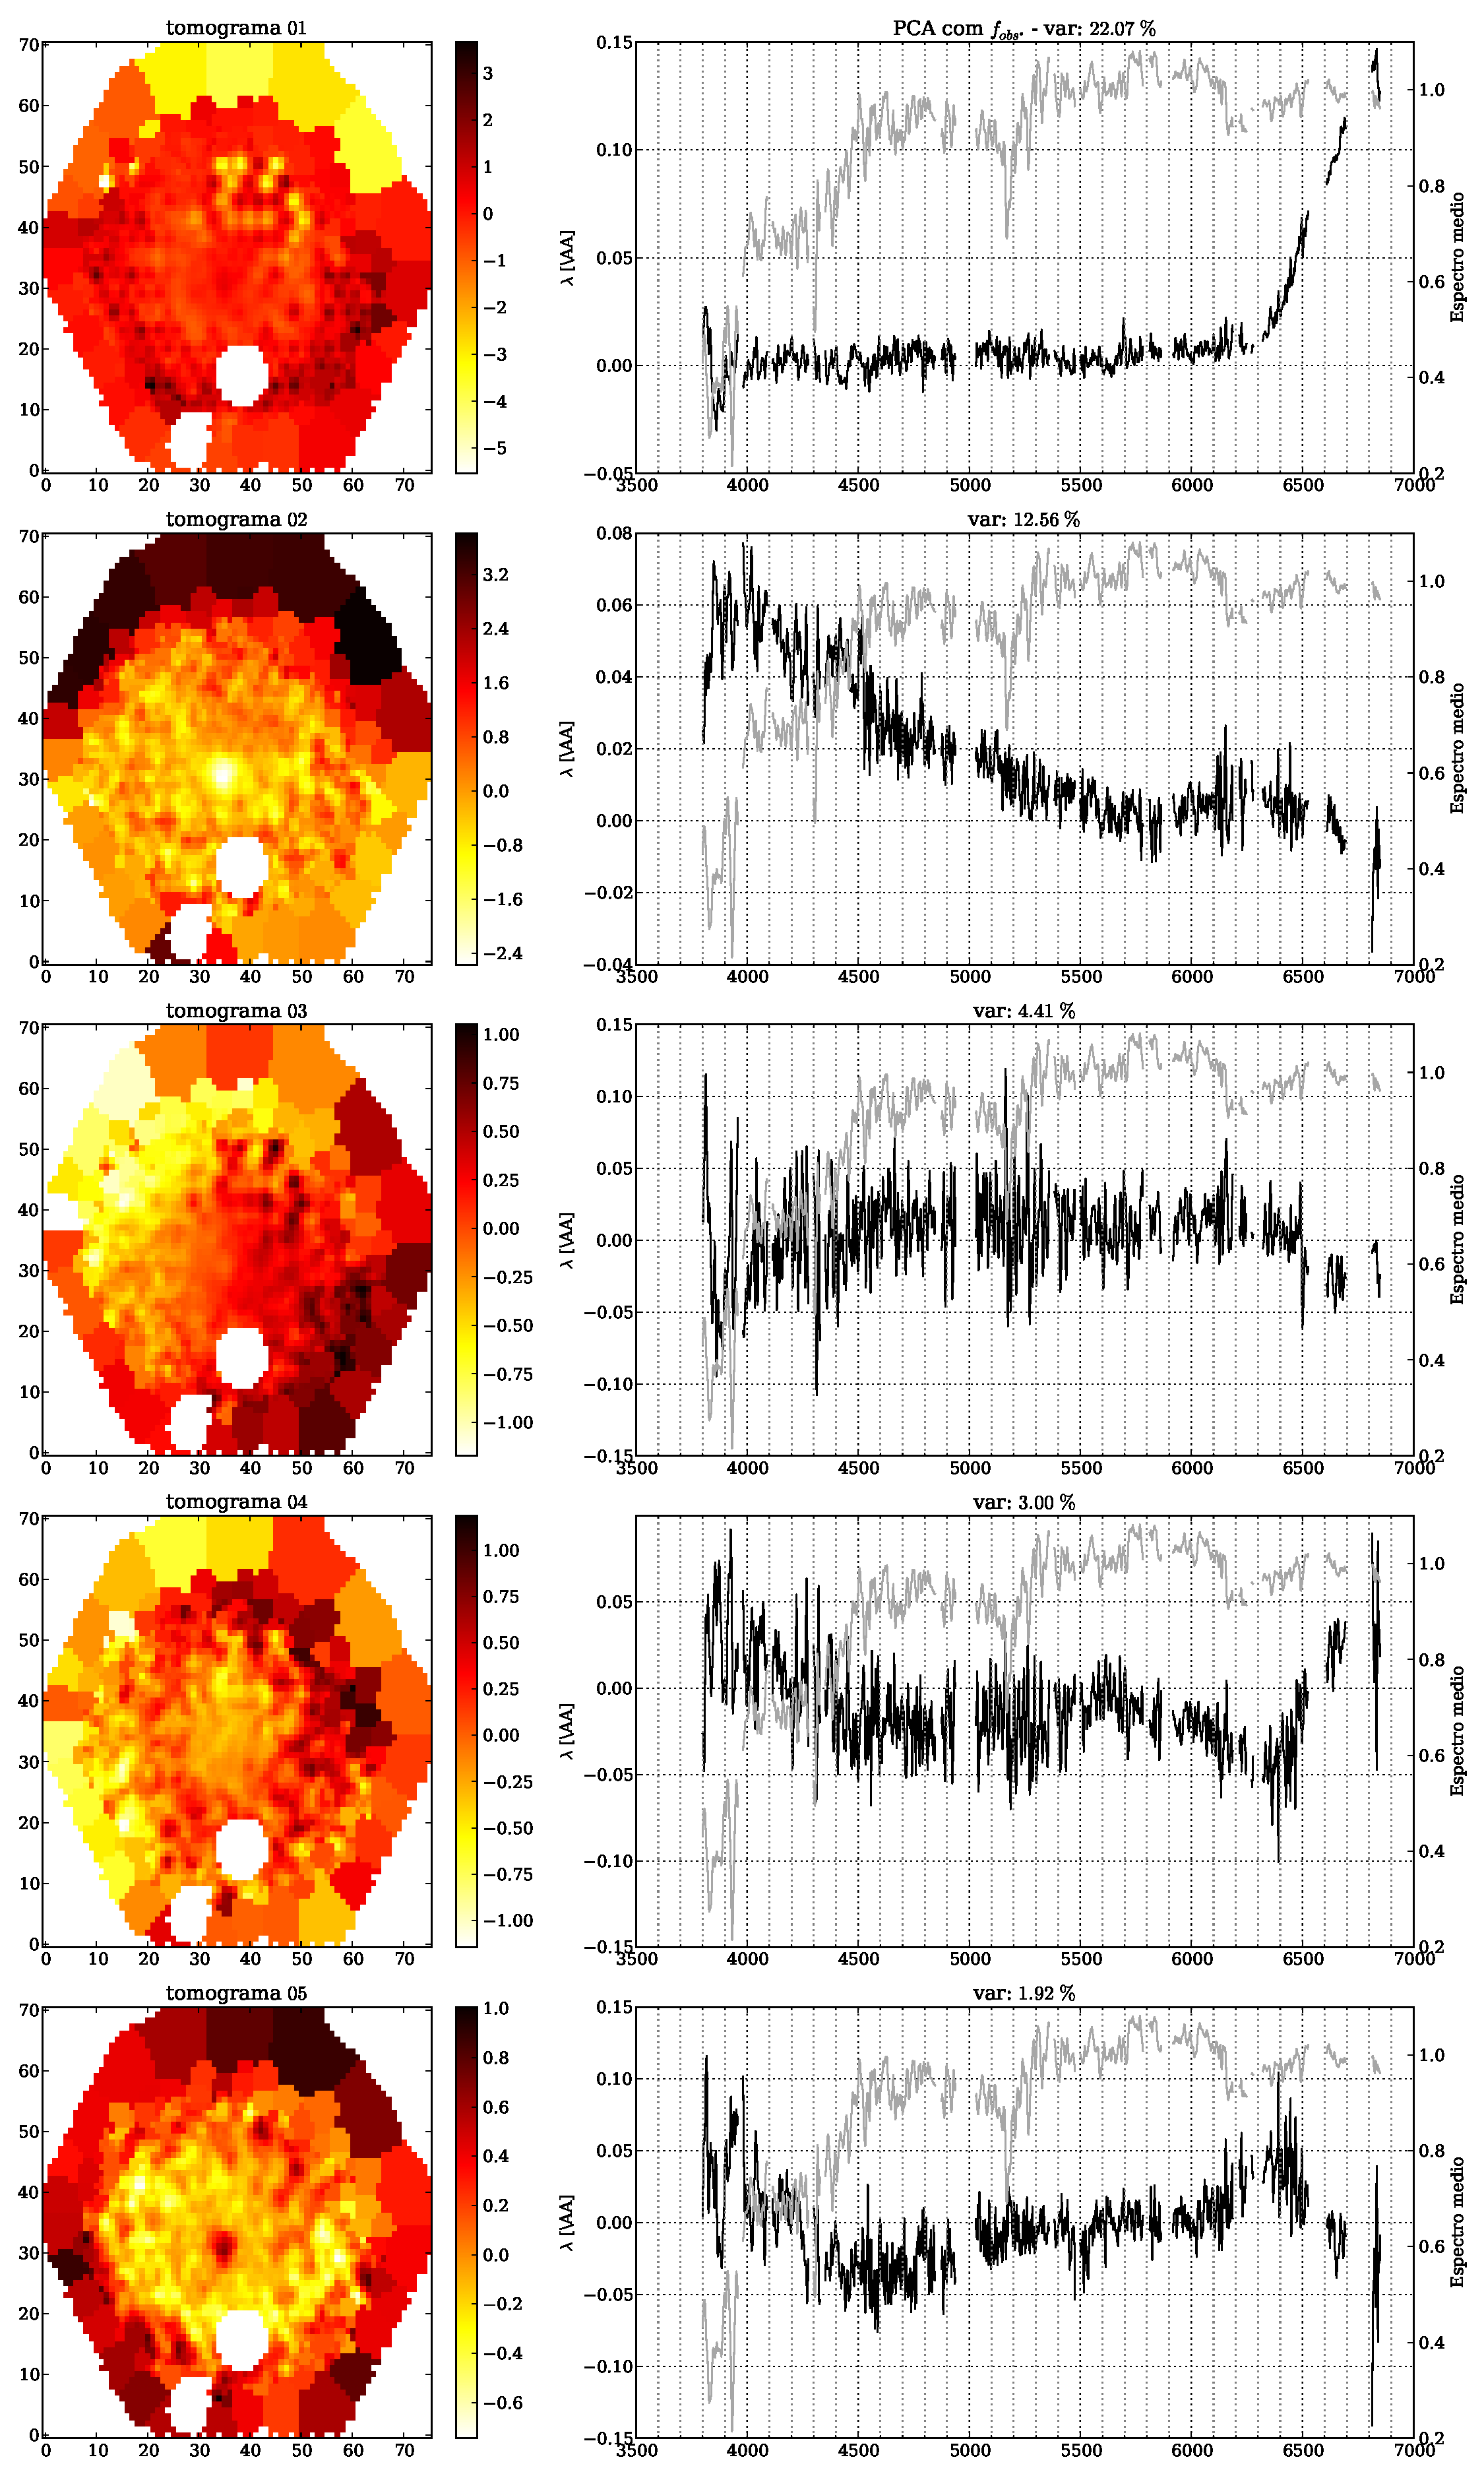
\includegraphics[width=0.8\textwidth]{figuras/K0119-tomo-obs-norm.pdf}
    \caption[Tomogramas de 1 a 5 para o cubo $f_{obs}$ - NGC 1167.]
    {Igual a Figura \ref{fig:K0008tomofobsnorm} para a galáxia NGC 1167.}
    \label{fig:K0119tomofobsnorm}
\end{figure}

\begin{figure}
    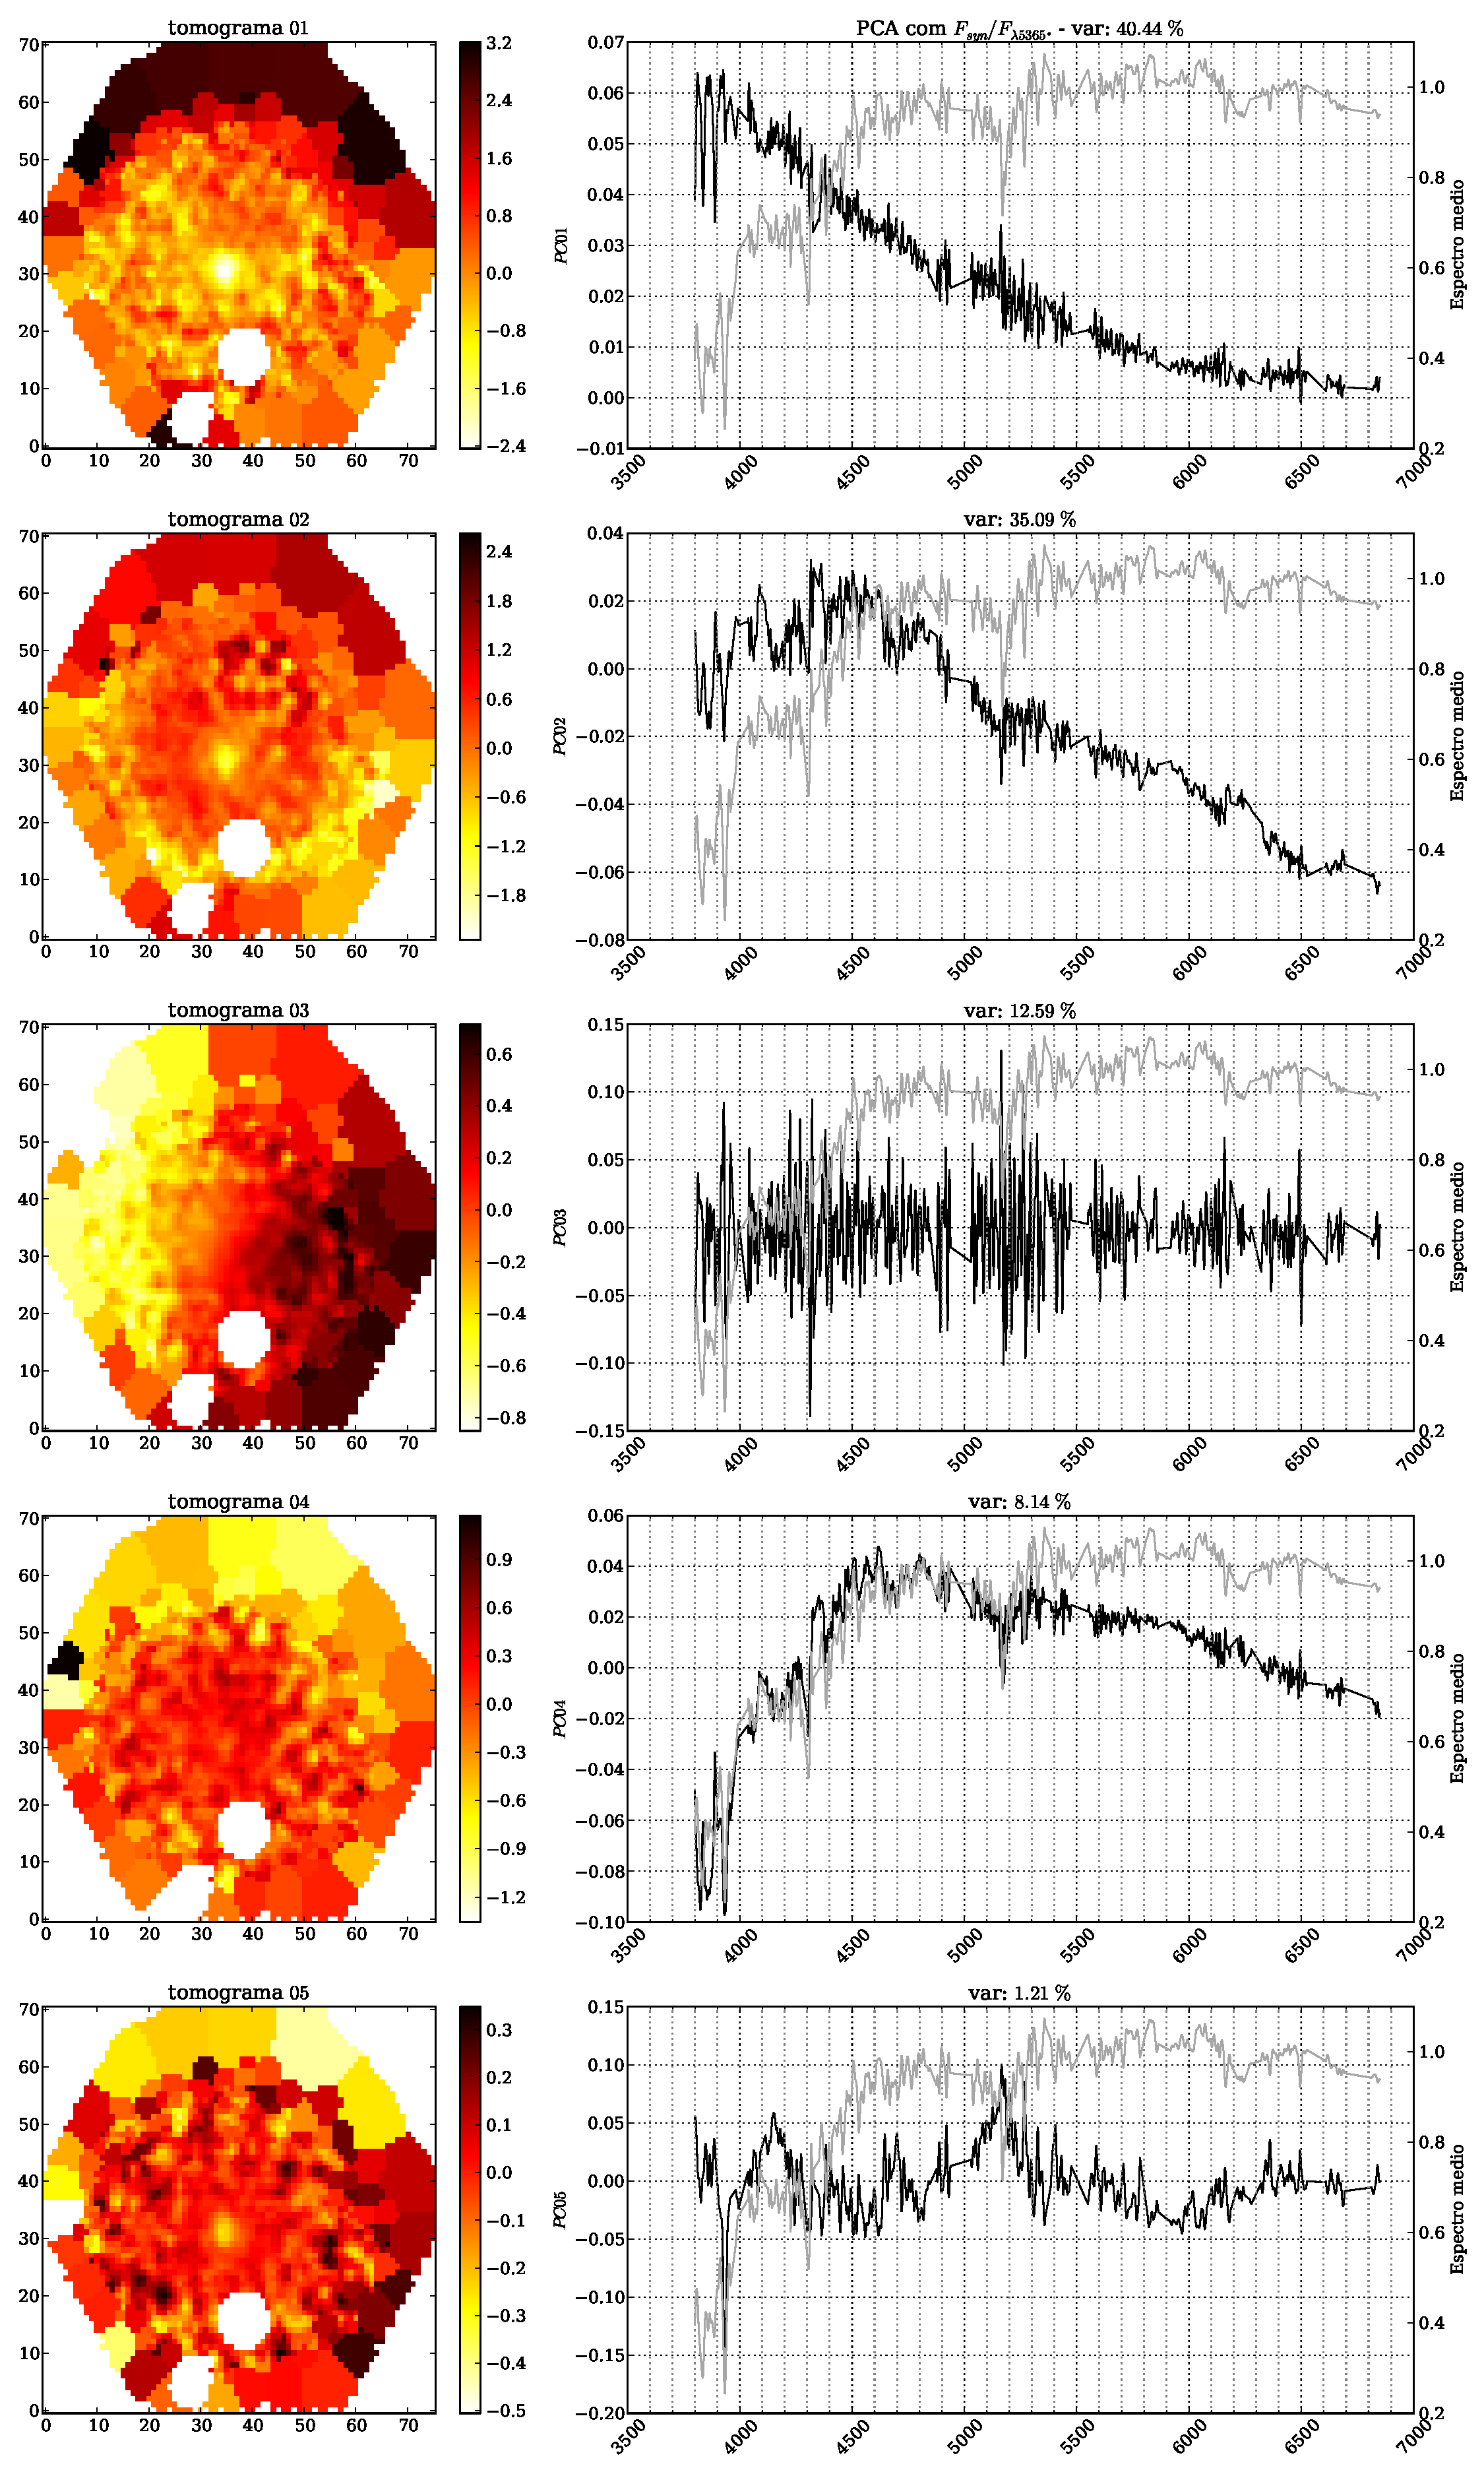
\includegraphics[width=0.8\textwidth]{figuras/K0119-tomo-syn-norm.pdf}
    \caption[Tomogramas de 1 a 5 para o cubo $f_{syn}$ - NGC 1167.]
    {Igual a Figura \ref{fig:K0008tomofsynnorm} para a galáxia NGC 1167.}
    \label{fig:K0119tomofsynnorm}
\end{figure}

\begin{figure}
    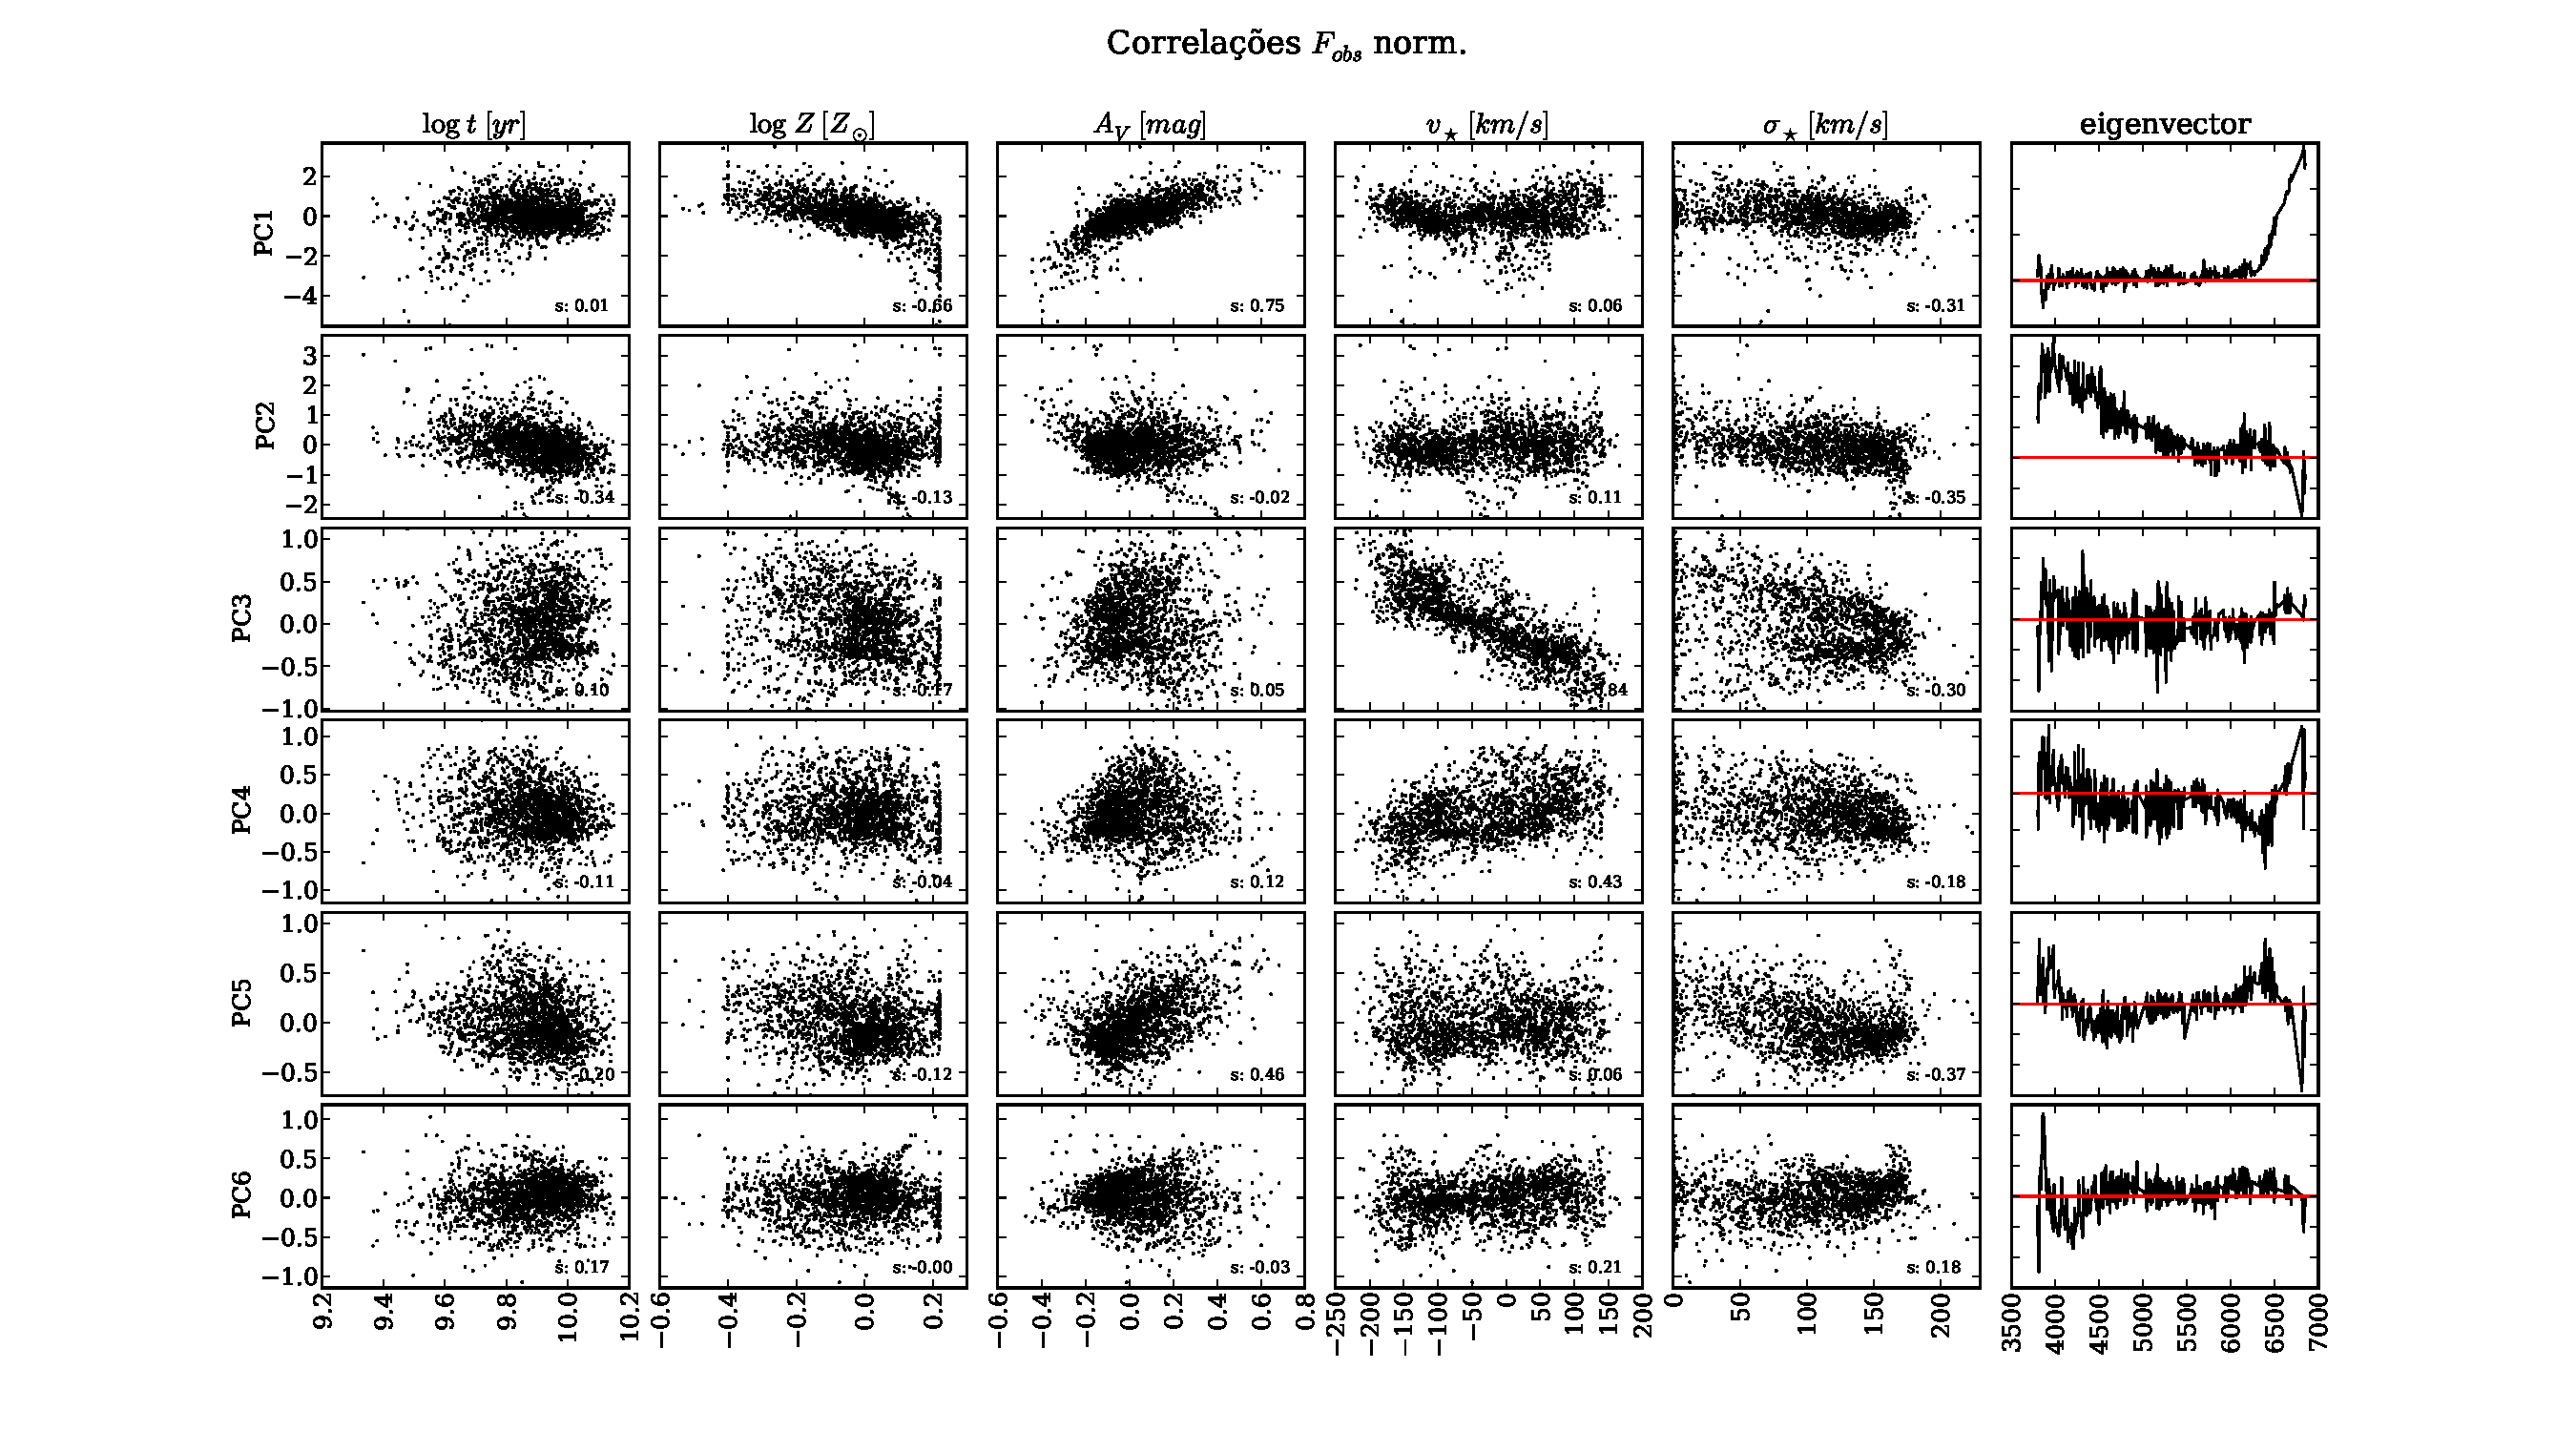
\includegraphics[width=1.2\textwidth, angle=-90]{figuras/K0119-correl-f_obs_norm-PCvsPhys.pdf}
	\caption[Correlações PCs vs. par\^ametros f\'isicos - $f_{obs}$ - NGC 1167.]
	{Igual a Figura \ref{fig:K0008correfobsnorm} para a galáxia NGC 1167.}
    \label{fig:K0119correfobsnorm}
\end{figure}

\begin{figure}
    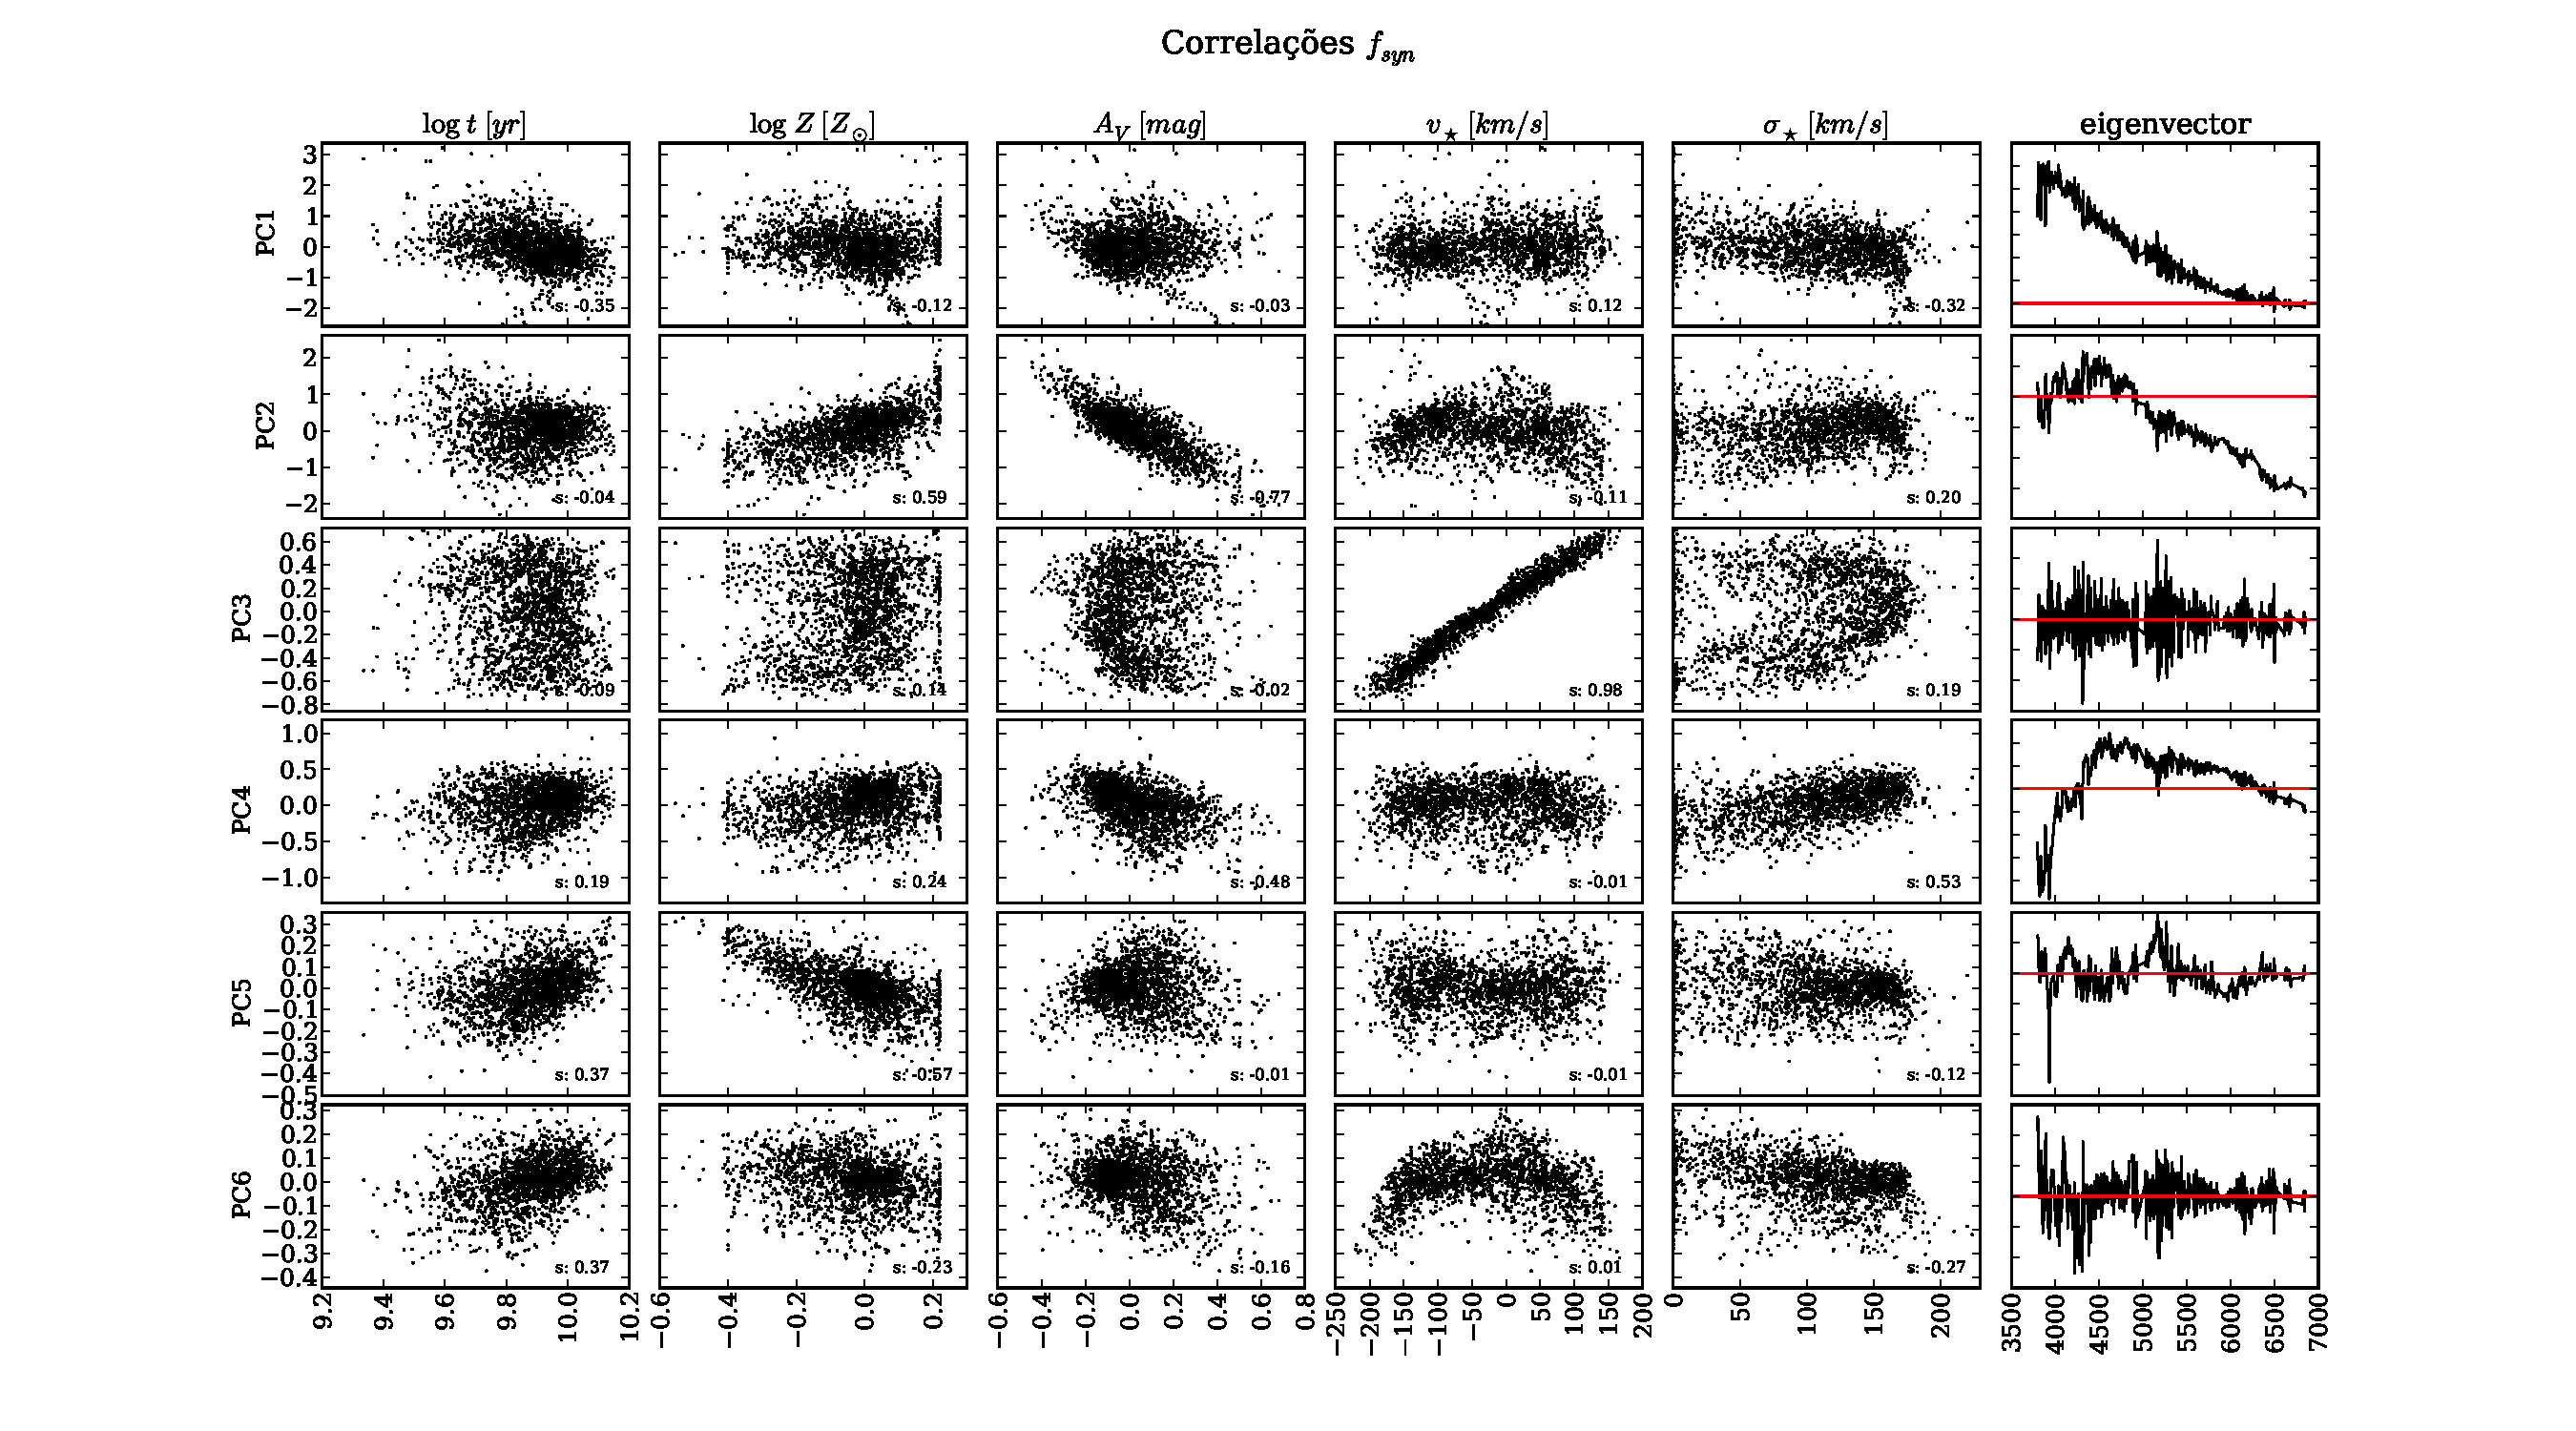
\includegraphics[width=1.2\textwidth, angle=-90]{figuras/K0119-correl-f_syn_norm-PCvsPhys.pdf}
	\caption[Correlações PCs vs. par\^ametros f\'isicos - $f_{syn}$ - NGC 1167.]
	{Igual a Figura \ref{fig:K0008correfsynnorm} para a galáxia NGC 1167.}
    \label{fig:K0119correfsynnorm}
\end{figure}

\subsection{NGC 6515 - CALIFA 864}

A primeira coisa que chama atenção nas imagens produzidas pelas propriedades físicas dessa galáxia elíptica é o número
de zonas faltantes na análise. Existem muitos objetos no {\em FoV} de observação dessa galáxia, portanto esses
``buracos'' são causados pelas máscaras espaciais criadas pelo {\sc qbick} conforme discutido na Seção
\ref{sec:CALePyC:pipelines}. O {\em scree test} (Figura \ref{fig:K0864scree}) possui o mesmo resultado assintótico das
outras galáxias, mas mostra uma variância percentual alta mesmo para componentes mais afastadas das cinco principais.

Analisando os tomogramas e PCs para o caso observado (Figura \ref{fig:K0864tomofobsnorm}) não parecem refletir
comportamentos físicos bem definidos. Podemos ver através das correlações (Figura \ref{fig:K0864correfobsnorm}) que não
está claro que exista alguma correlação singular, salvo PC1 e talvez a PC3. A PC1 correlaciona com $A_V$ e a PC3 com a
dispersão de velocidades ($\sigma_\star$), mas nada muito notável. Para o caso sintético (tomogramas e PCs na Figura
\ref{fig:K0864tomofobsnorm} e correlações na Figura \ref{fig:K0864correfsynnorm}) temos uma correlação da PC1 com $A_V$
também, mas temos umas correlações mais fortes. A PC3 correlaciona com quase tudo, o que mostra que ela deve ser um tipo
de fator de escala que segue o mesmo gradiente das demais propriedades físicas. Nessa PC ainda podemos ver que para a
dispersão de velocidades a correlação é um pouco mais alta ($s\ =\ 0.62$). A PC4 possui o mesmo padrão de correlações
distribuidas entre as propriedades, mas é mais notável a correlação com a velocidade estelar ($v_\star$), o que fica
claro também observando a PC (autoespectro) que possui um padrão de oscilação em torno do zero. Detalhe para a PC6 que
possui forte correlação com idade e metalicidade.

\begin{figure}
    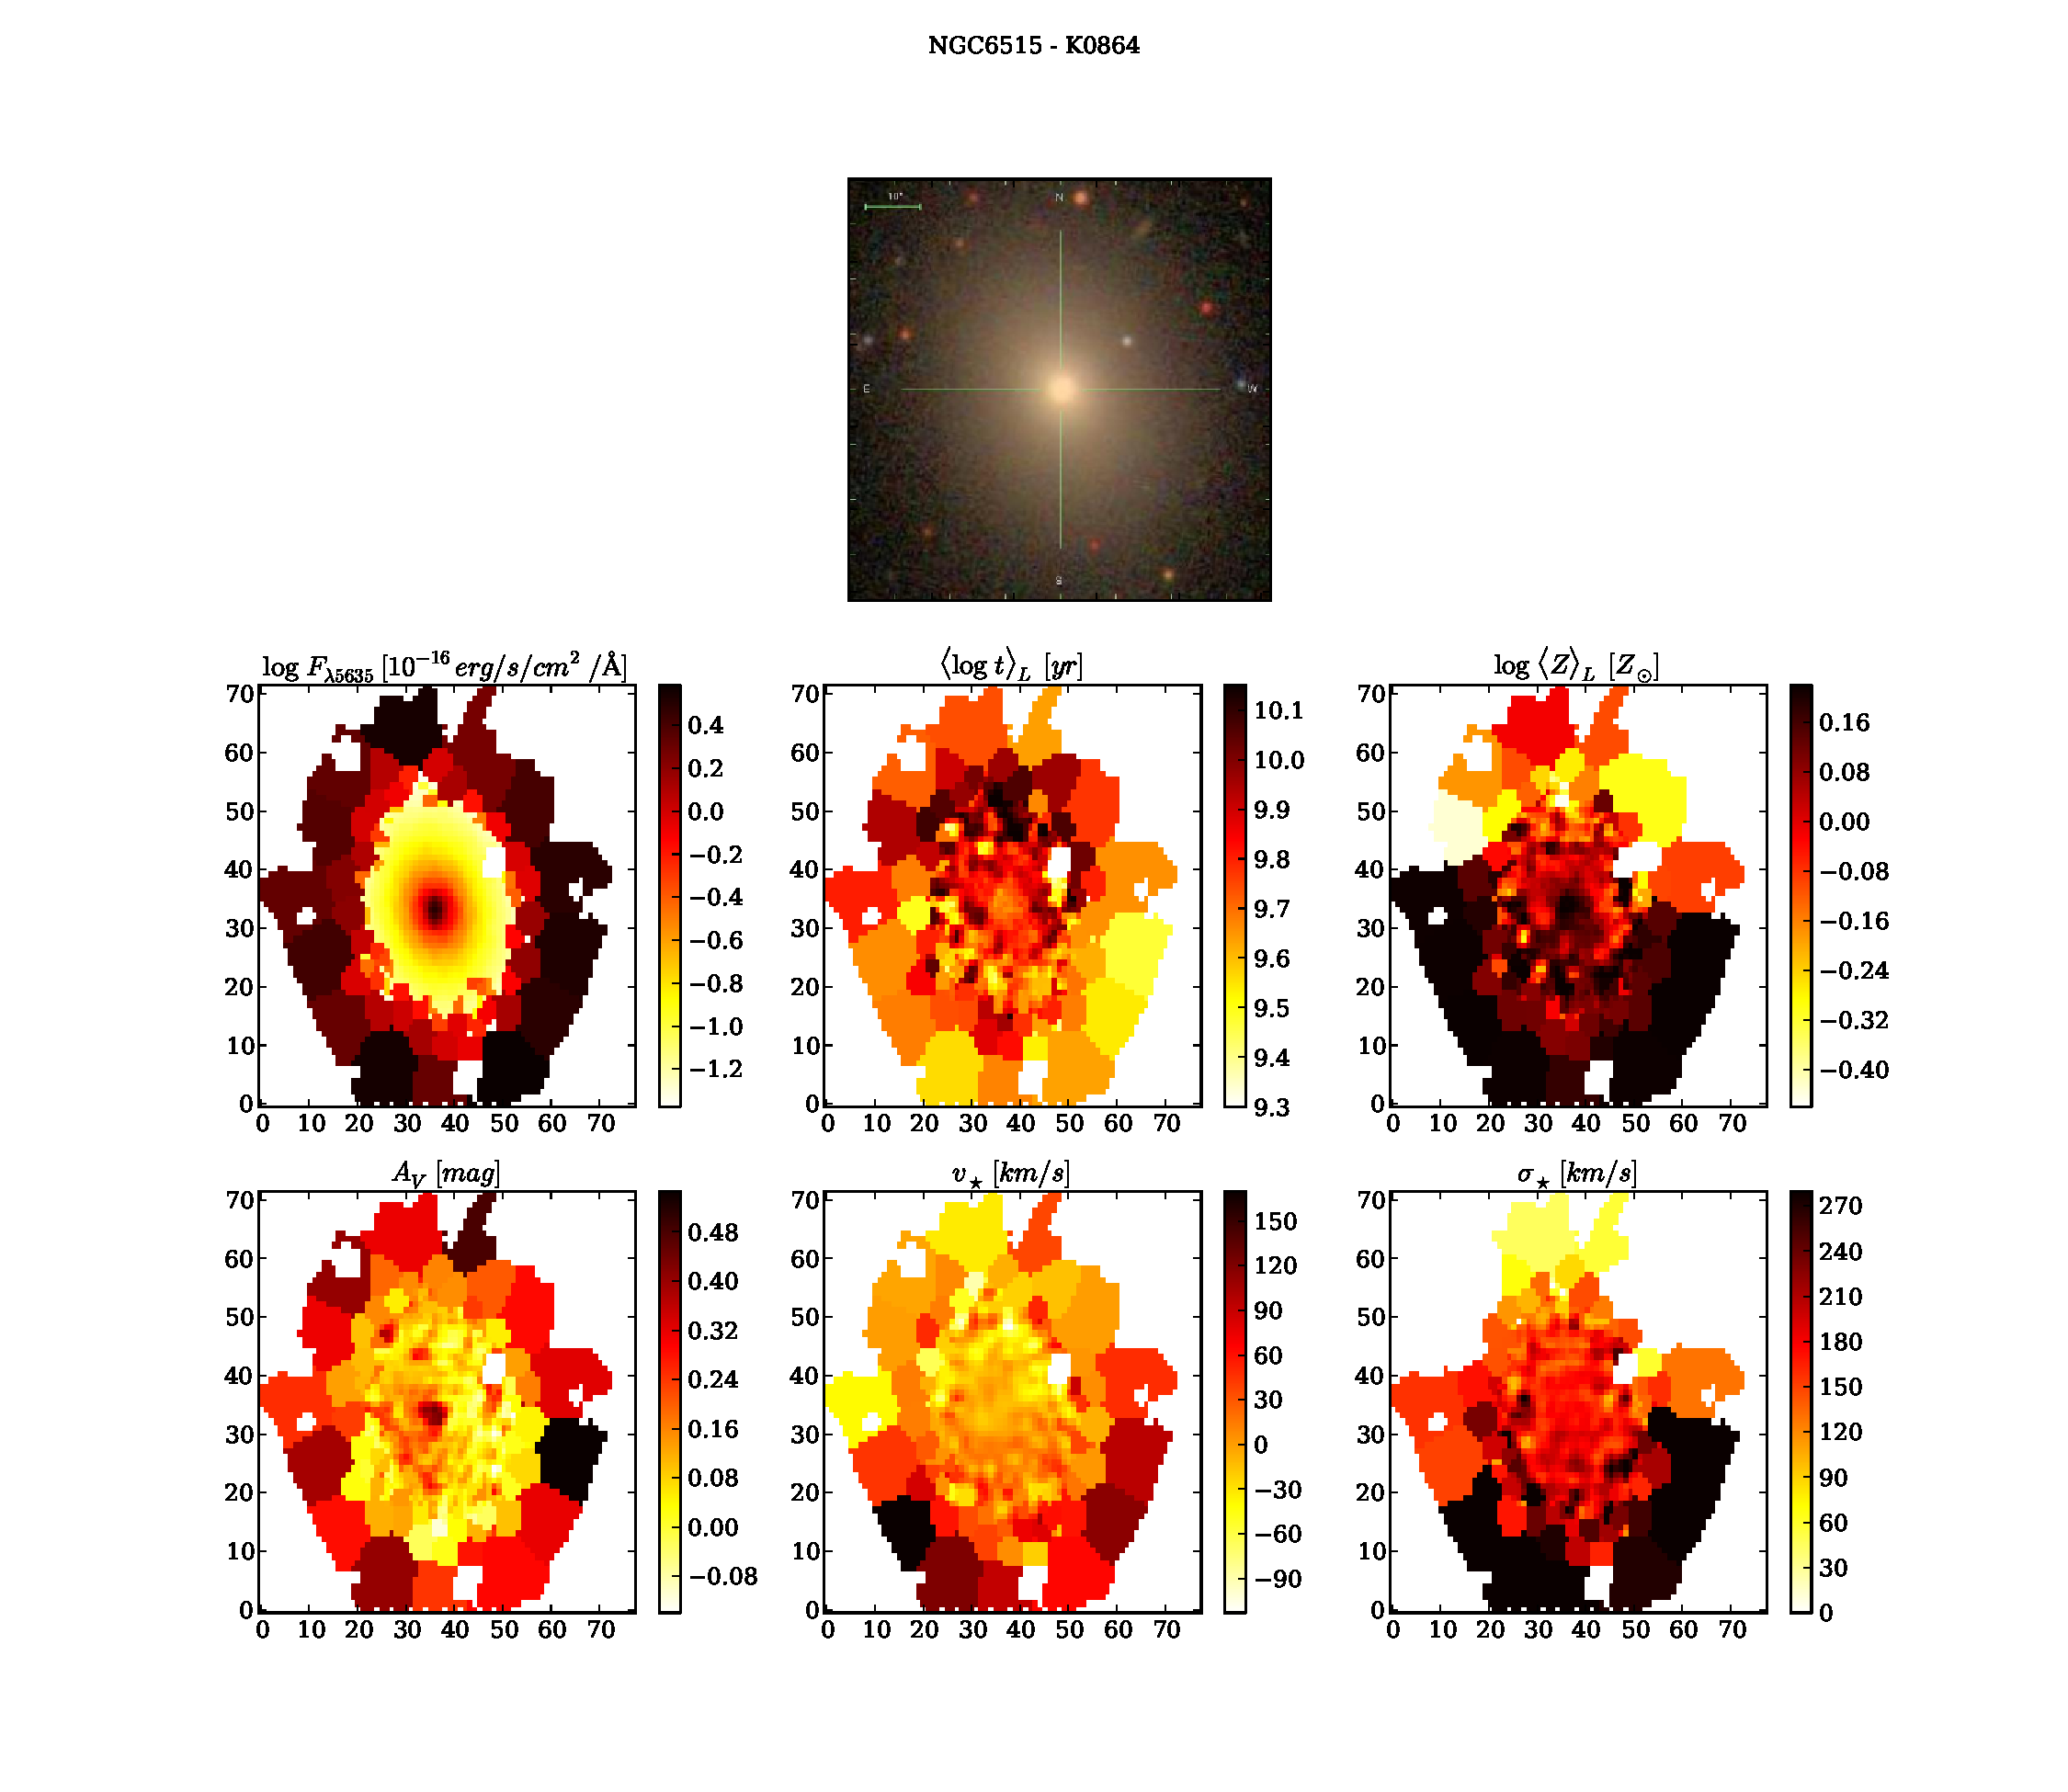
\includegraphics[width=1.\textwidth]{figuras/K0864-apresent.pdf}
    \caption[Propriedades f\'isicas da gal\'axia NGC 6515.]
    {Igual a Figura \ref{fig:K0008apresent} para a galáxia NGC 6515.}
    \label{fig:K0864apresent}
\end{figure}

\begin{figure}
    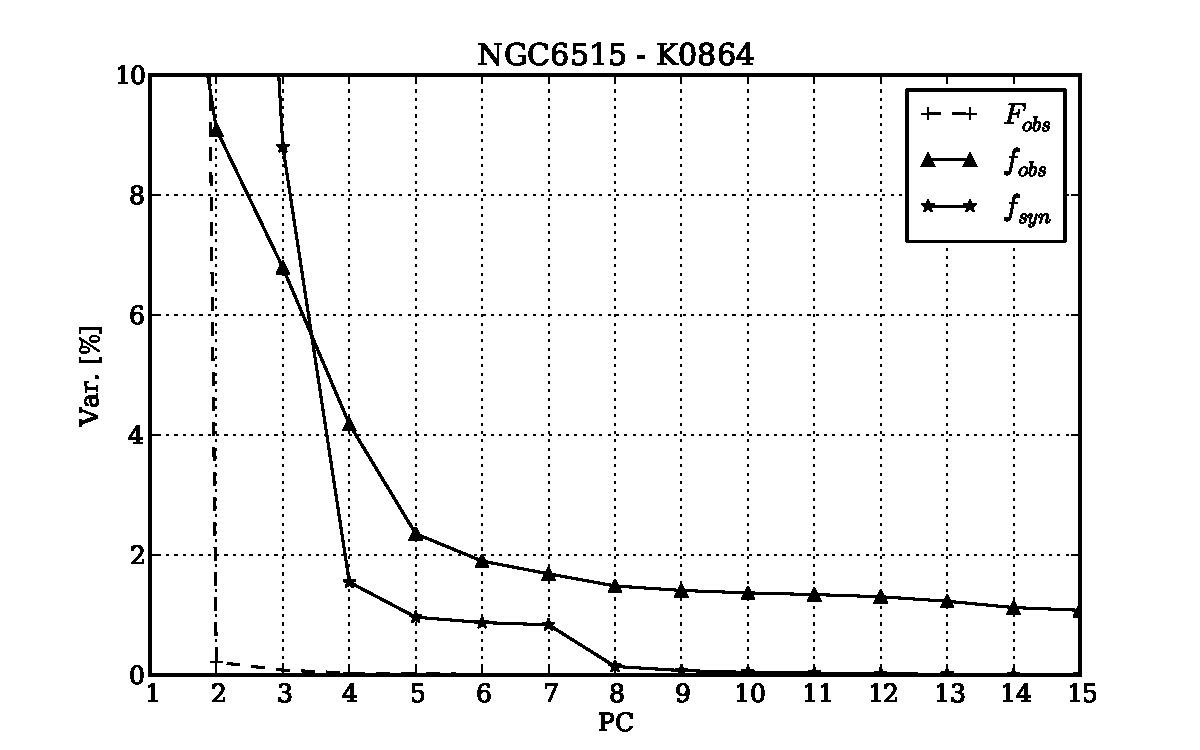
\includegraphics[height=0.33\textheight]{figuras/K0864-screetest.pdf}
    \caption[Scree test comparativo entre 3 PCAs - NGC 6515.]
	{Igual a Figura \ref{fig:K0008scree} para a galáxia NGC 6515.}
    \label{fig:K0864scree}
\end{figure}

\begin{figure}
    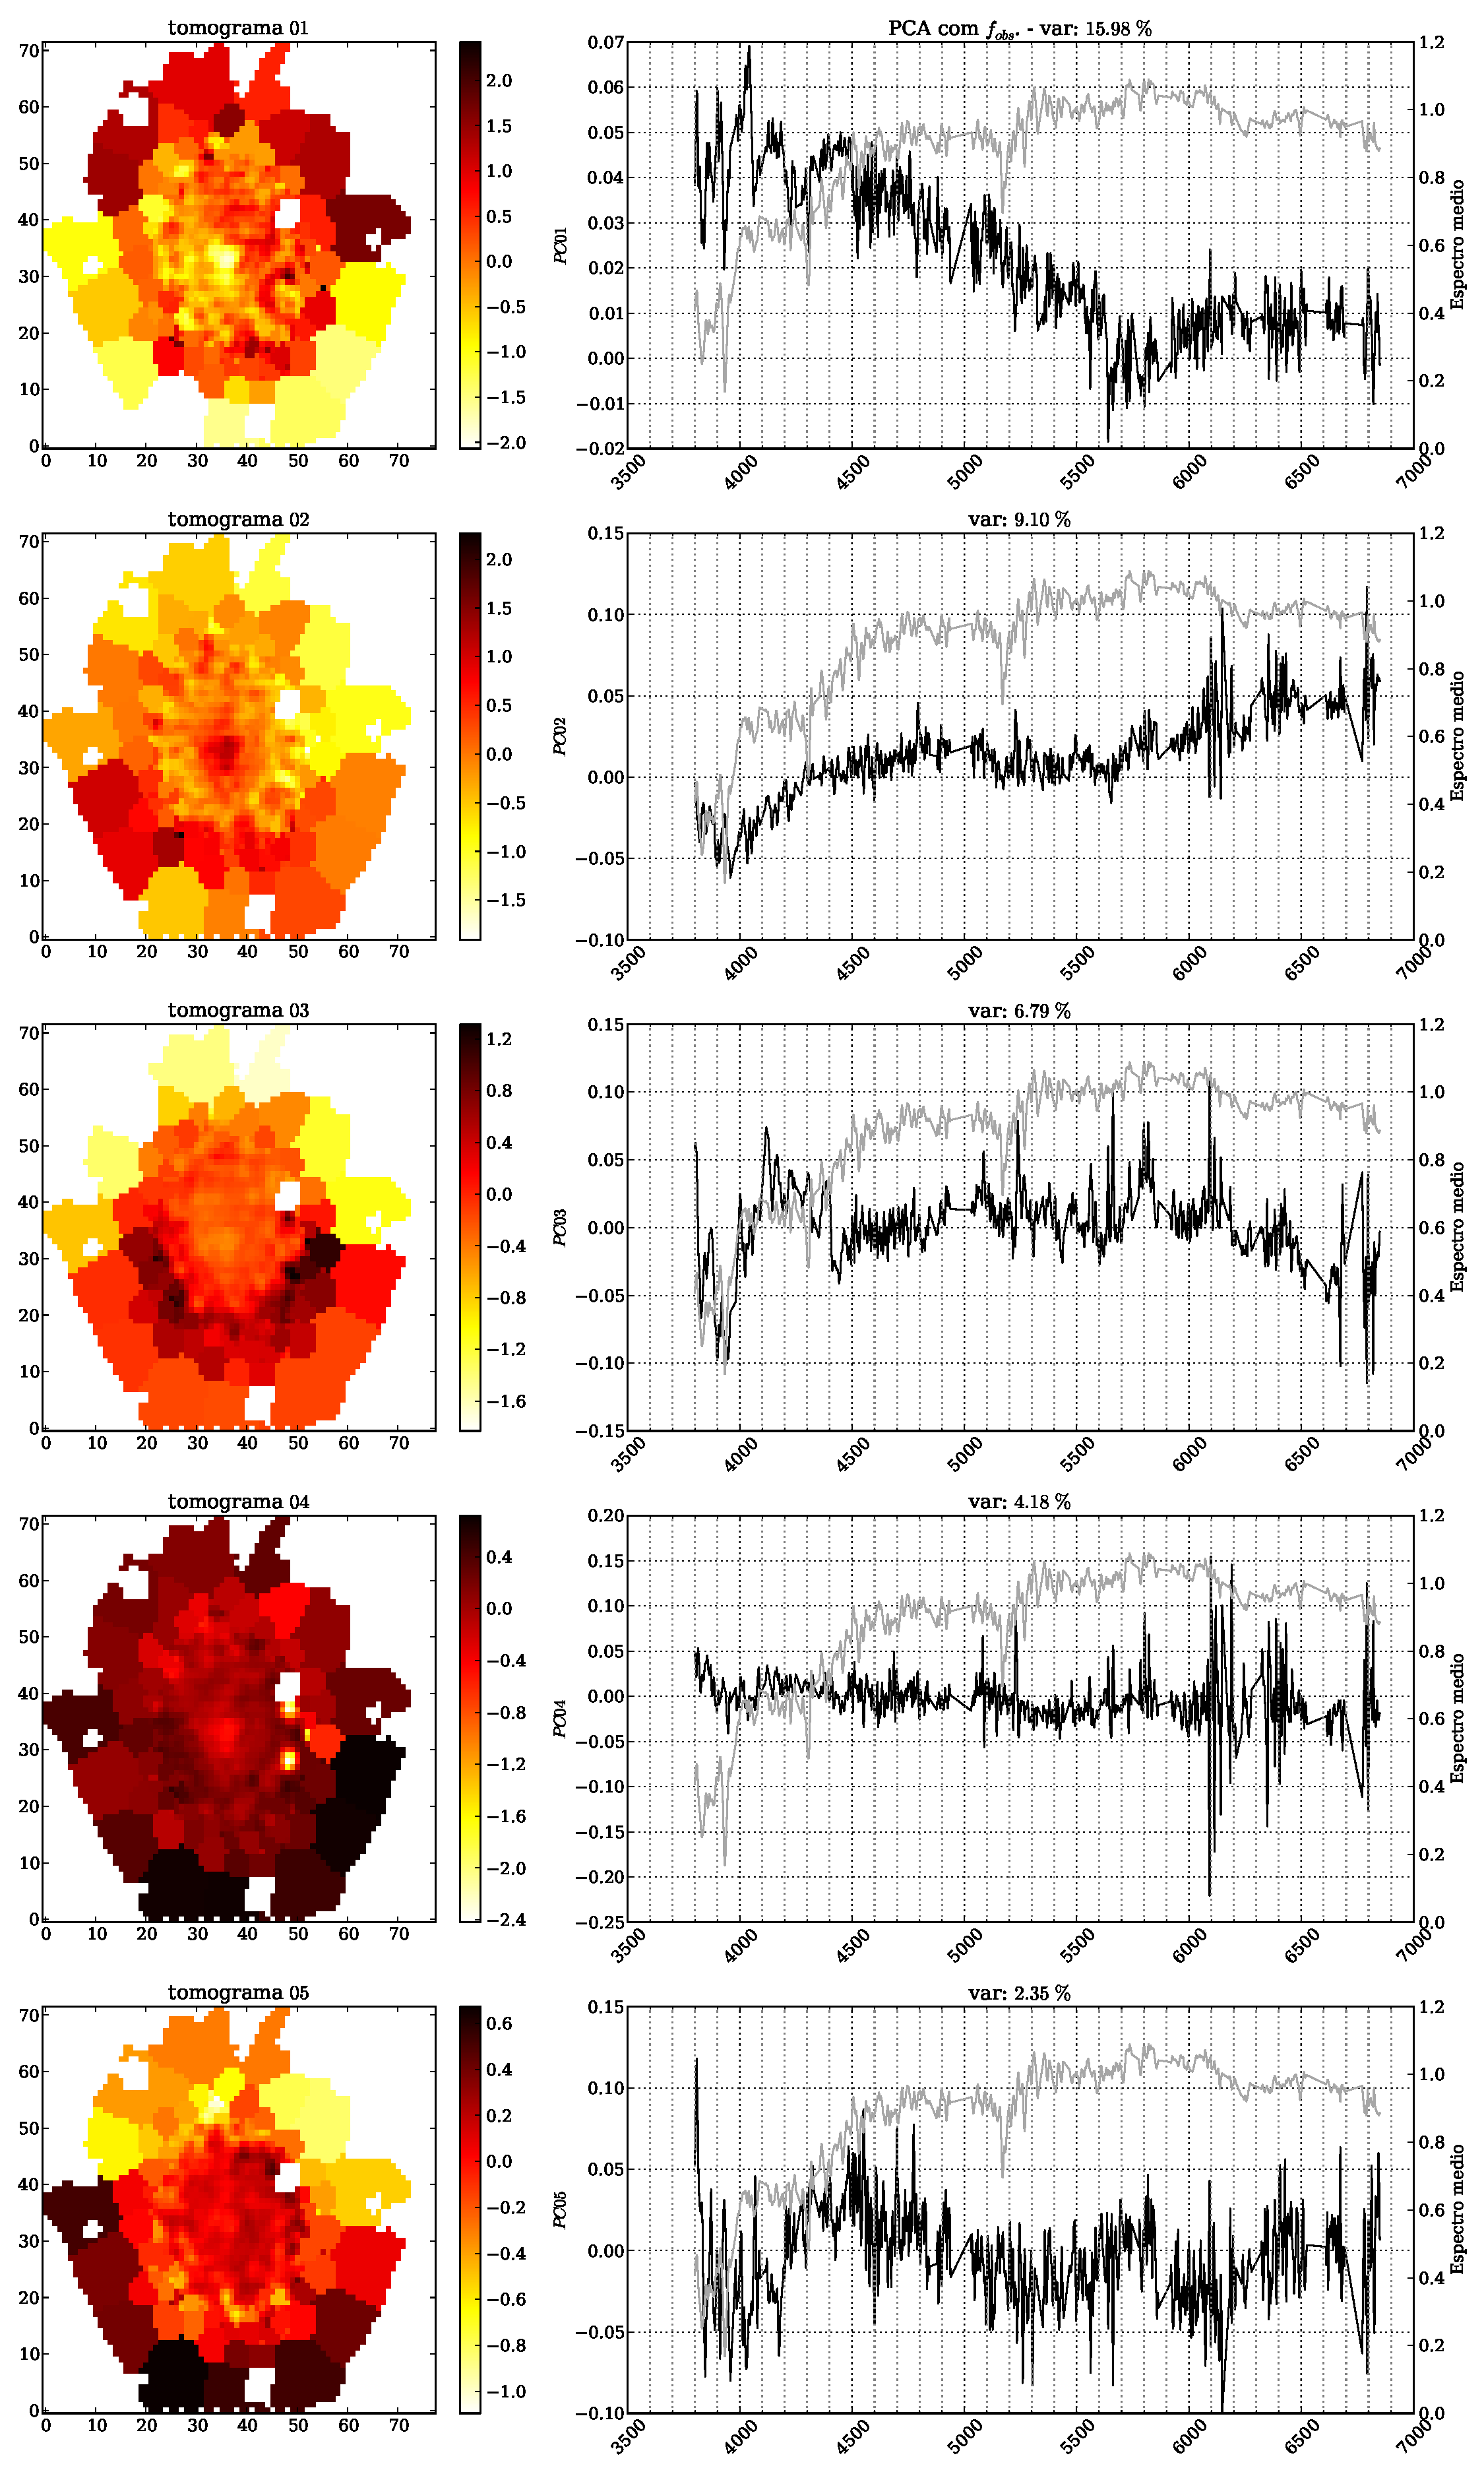
\includegraphics[width=0.8\textwidth]{figuras/K0864-tomo-obs-norm.pdf}
    \caption[Tomogramas de 1 a 5 para o cubo $f_{obs}$ - NGC 6515.]
    {Igual a Figura \ref{fig:K0008tomofobsnorm} para a galáxia NGC 6515.}
    \label{fig:K0864tomofobsnorm}
\end{figure}

\begin{figure}
    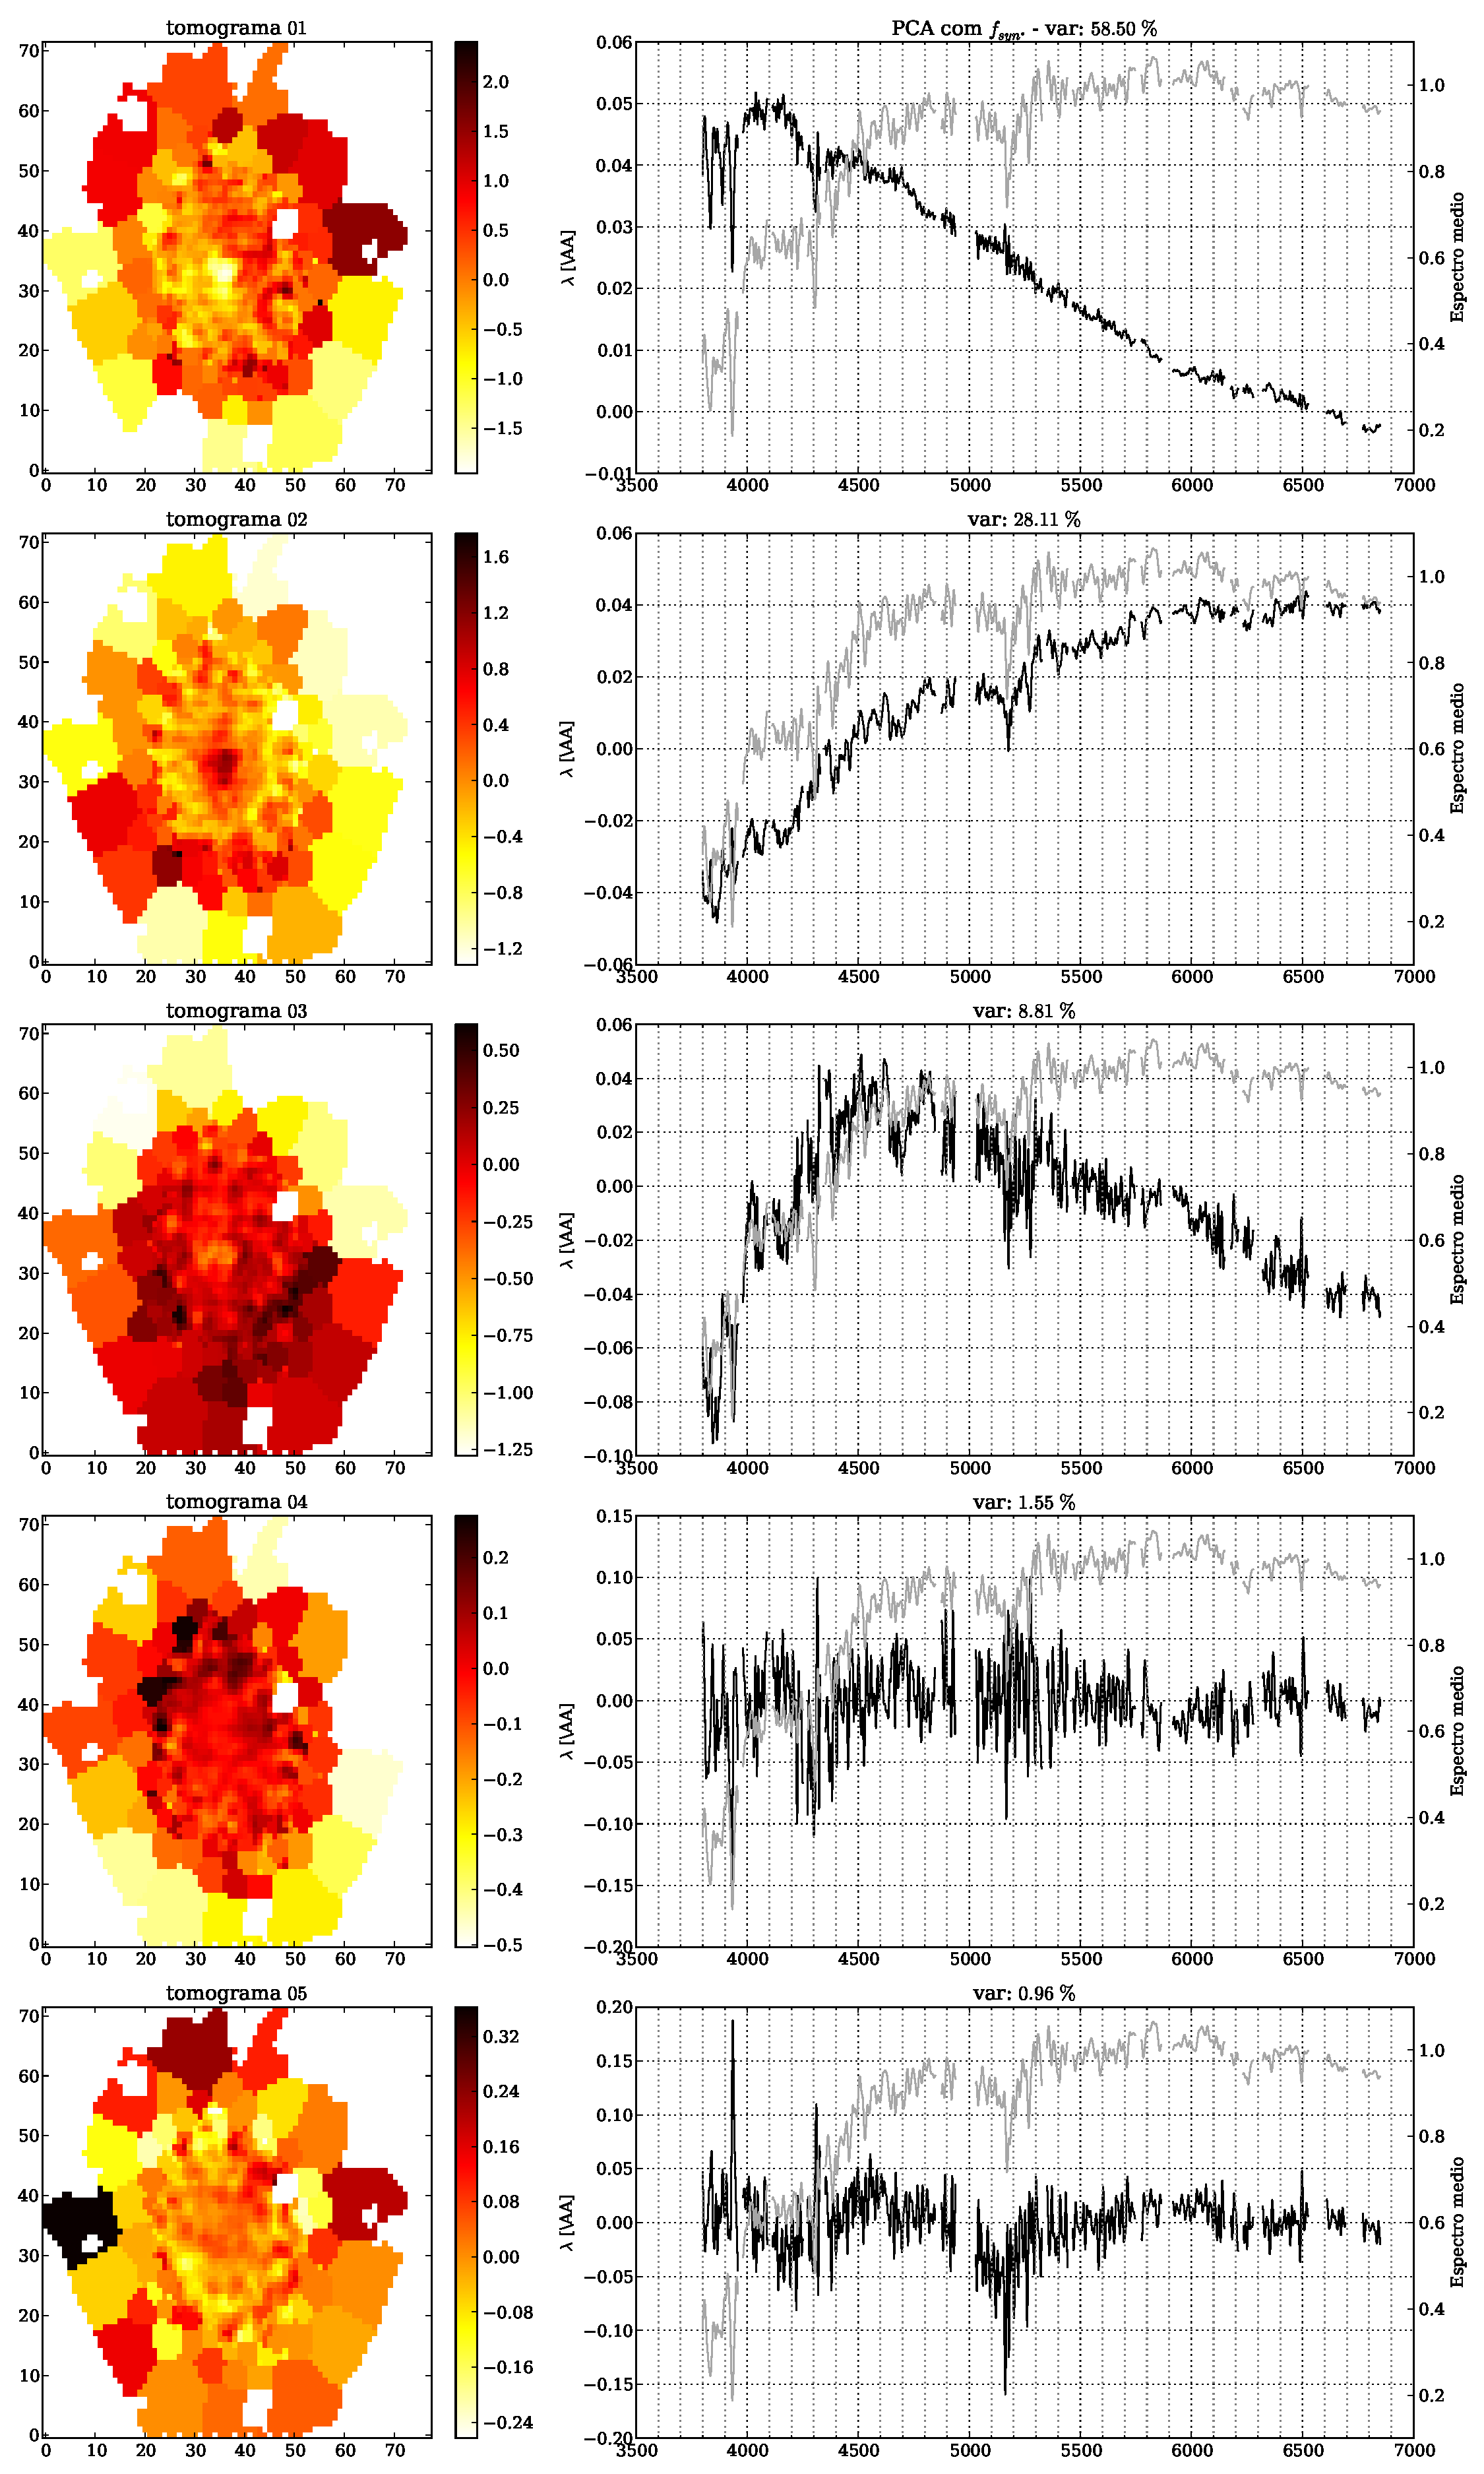
\includegraphics[width=0.8\textwidth]{figuras/K0864-tomo-syn-norm.pdf}
    \caption[Tomogramas de 1 a 5 para o cubo $f_{syn}$ - NGC 6515.]
    {Igual a Figura \ref{fig:K0008tomofsynnorm} para a galáxia NGC 6515.}
    \label{fig:K0864tomofsynnorm}
\end{figure}

\begin{figure}
    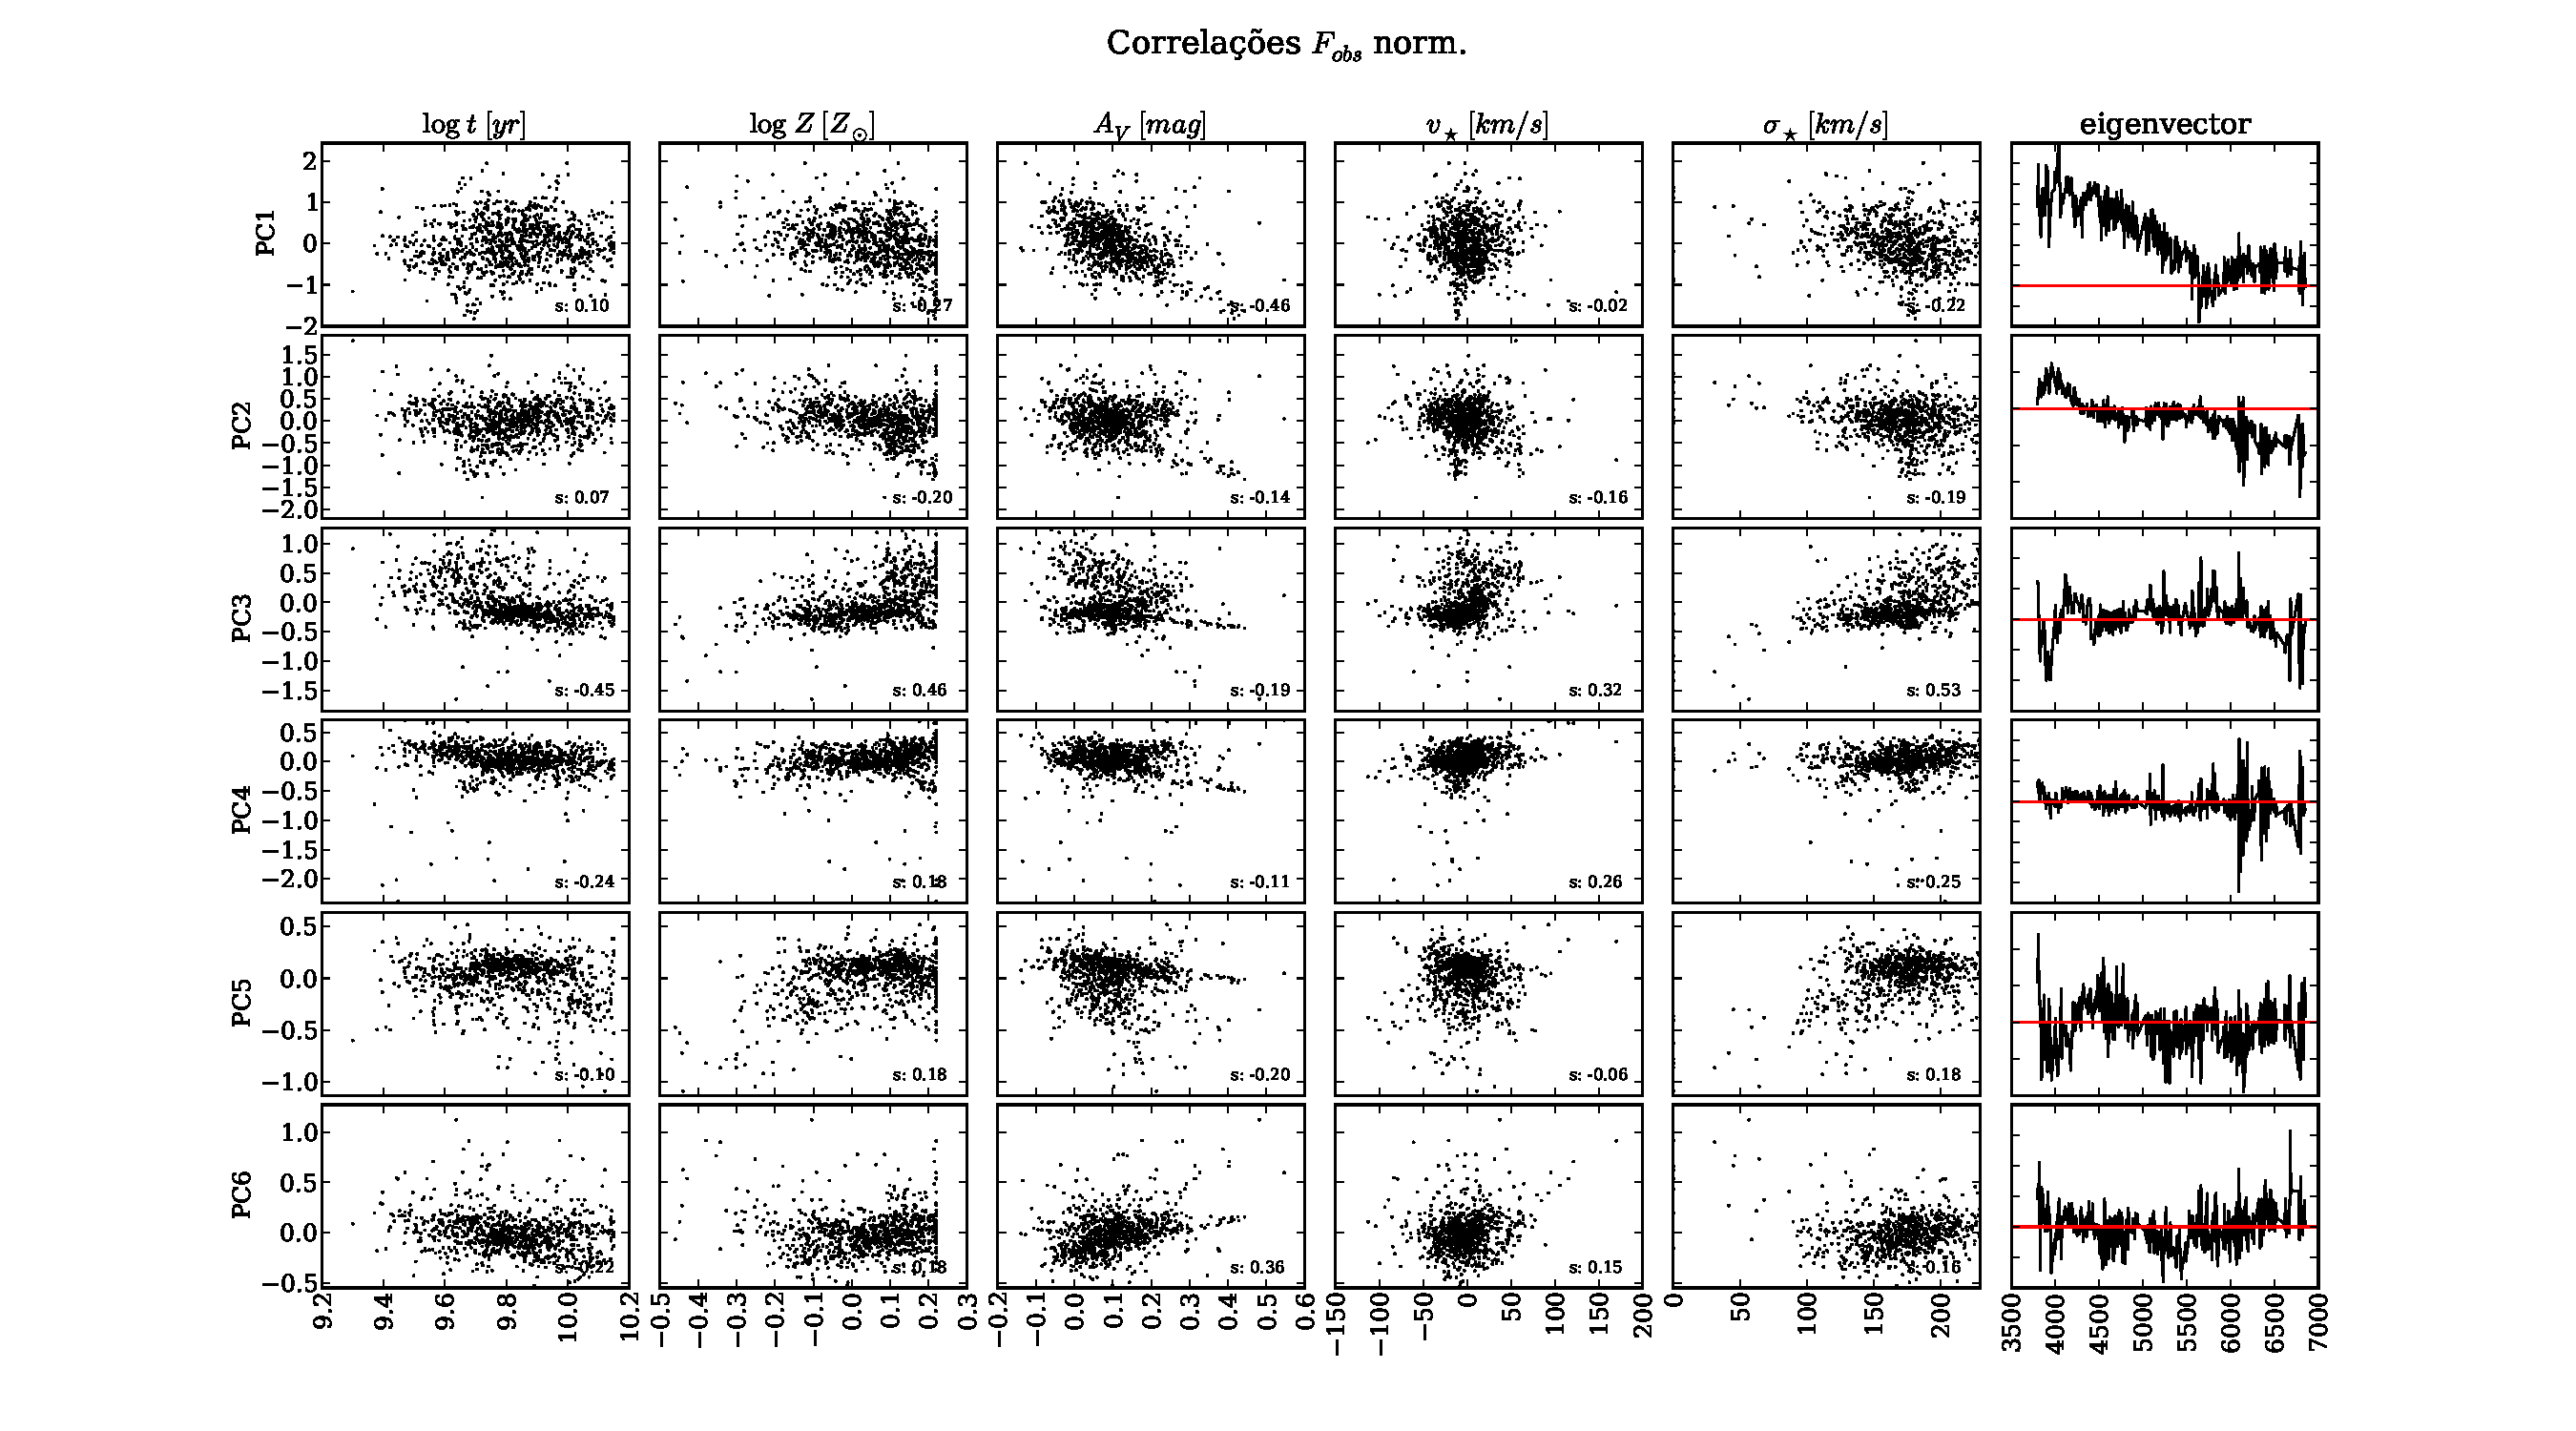
\includegraphics[width=1.2\textwidth, angle=-90]{figuras/K0864-correl-f_obs_norm-PCvsPhys.pdf}
	\caption[Correlações PCs vs. par\^ametros f\'isicos - $f_{obs}$ - NGC 6515.]
	{Igual a Figura \ref{fig:K0008correfobsnorm} para a galáxia NGC 6515.}
    \label{fig:K0864correfobsnorm}
\end{figure}

\begin{figure}
    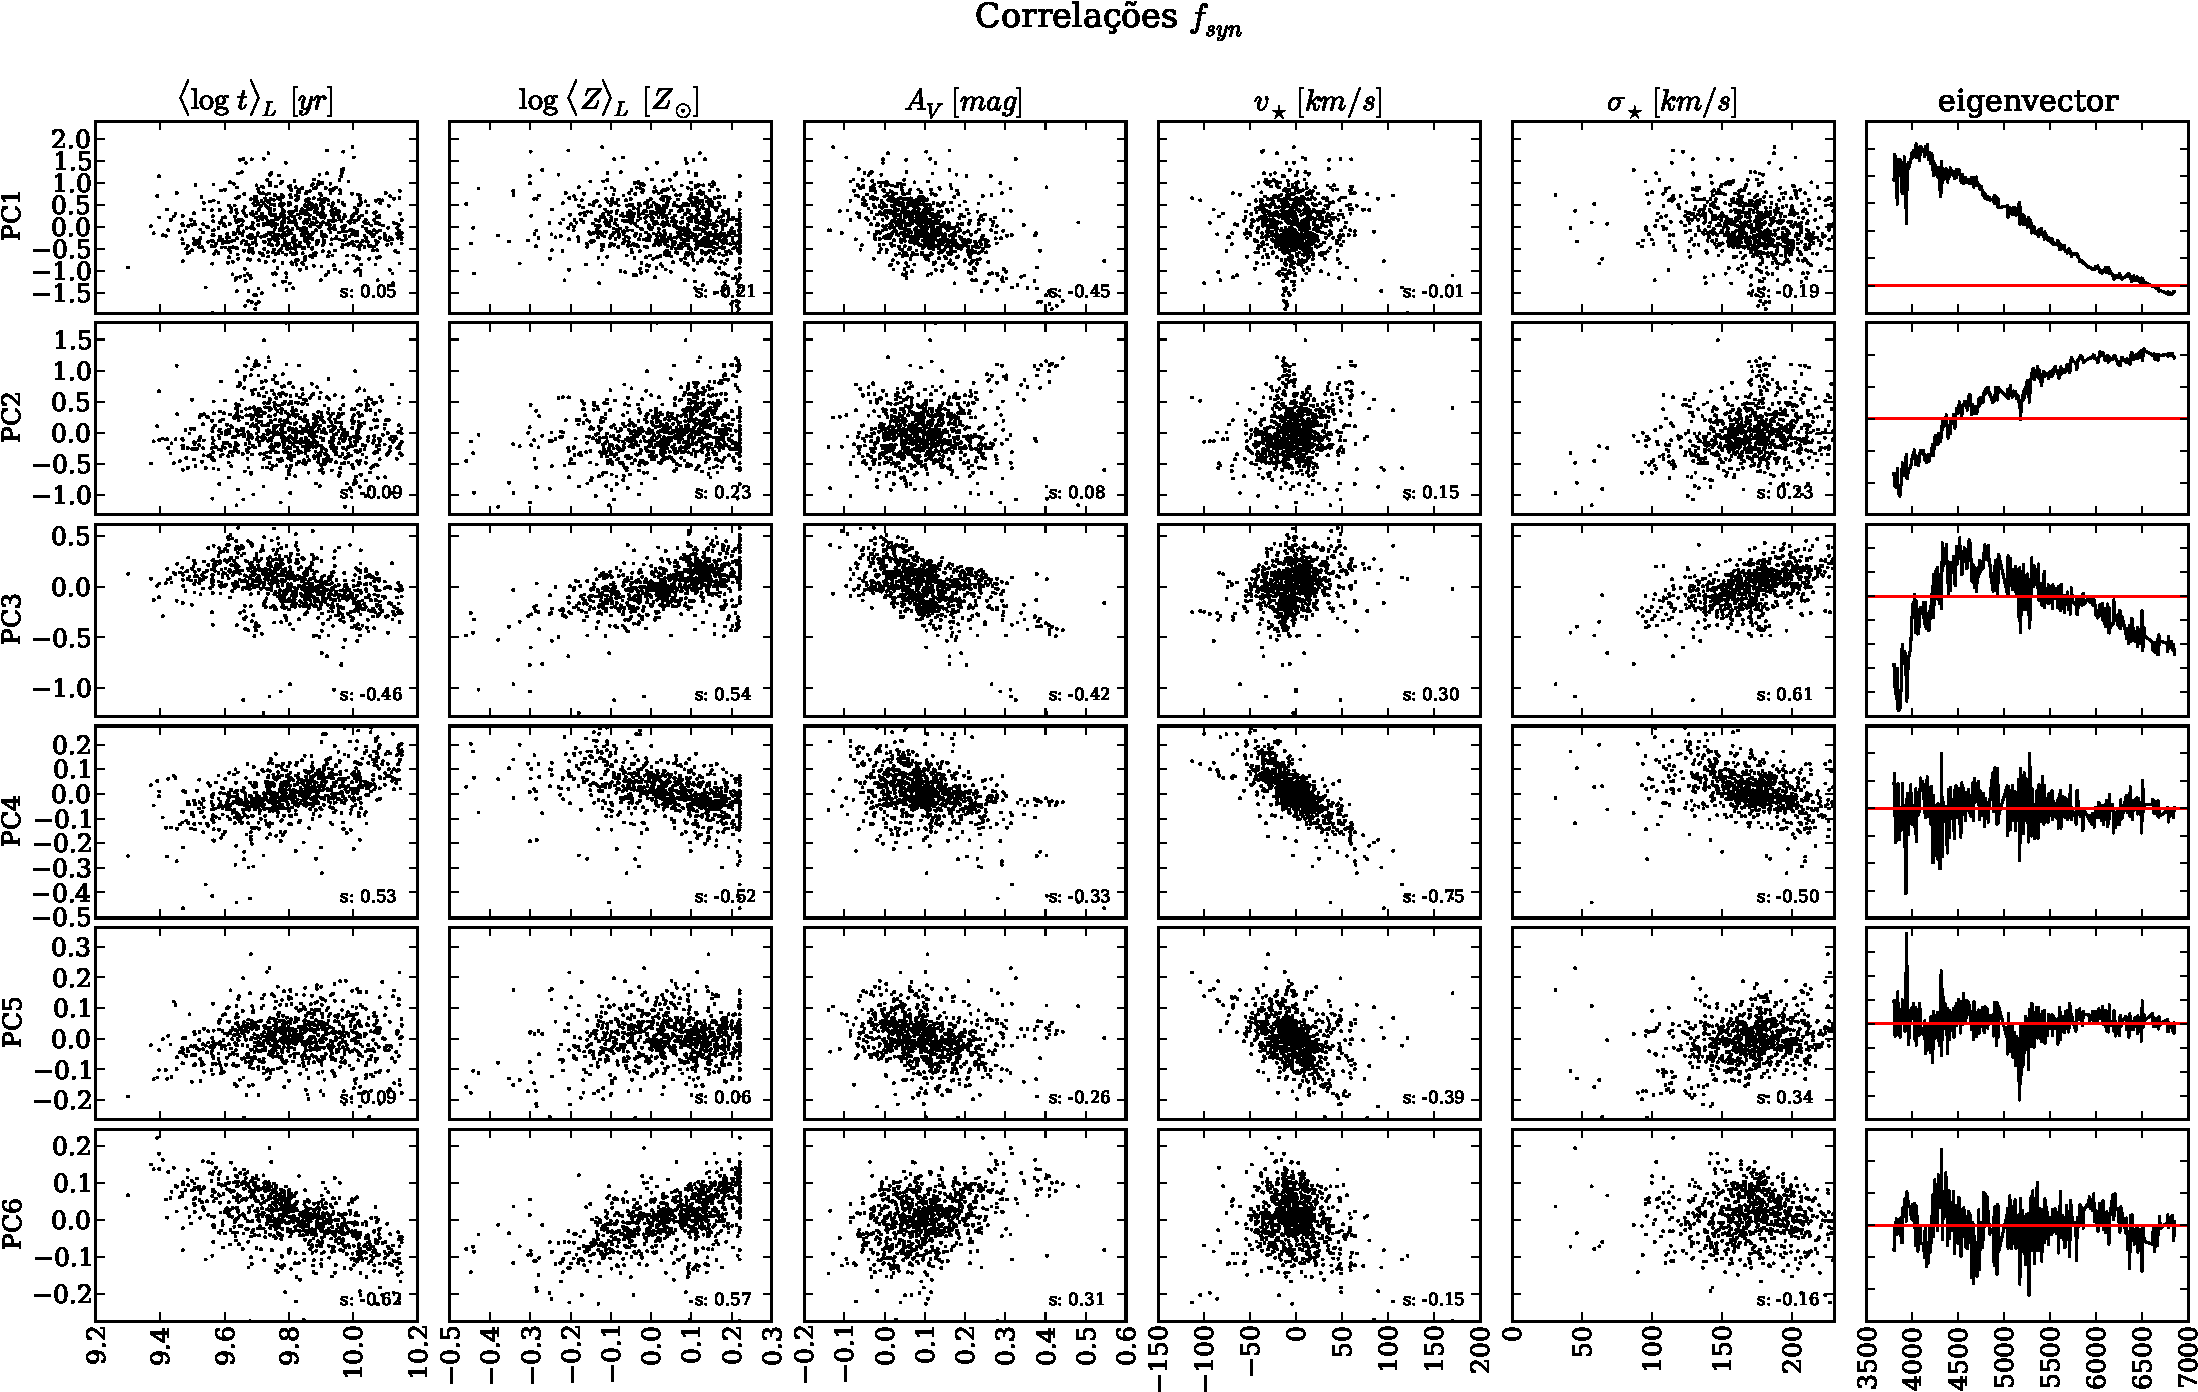
\includegraphics[width=1.2\textwidth, angle=-90]{figuras/K0864-correl-f_syn_norm-PCvsPhys.pdf}
	\caption[Correlações PCs vs. par\^ametros f\'isicos - $f_{syn}$ - NGC 6515.]
	{Igual a Figura \ref{fig:K0008correfsynnorm} para a galáxia NGC 6515.}
    \label{fig:K0864correfsynnorm}
\end{figure}

\section{{\em Mergers}}
\label{sec:result:mergers}

Se para galáxias {\em early-type} esperávamos (e observamos) uma certa homgeneidade nas distribuições espaciais de PCs e
propriedades físicias, o contrário acontece no caso de {\em mergers}. Estes objetos complexos representam misturas de
duas galáxias, às quais se adiciona toda "confusão" gerada pela concentracao de gás e poeira e a formação estelar
resultante. Nessa seção analisaremos dois sistemas desse tipo.

\subsection{NGC 2623 - CALIFA 213}

Quando olhamos a figura de apresentação da imagem e das propriedades da galáxia NGC 2623 (Figura
\ref{fig:K0213apresent}) fica evidente a natureza irregular e a diferença na distribuição espacial da idade média das
populações estelares. Seu {\em scree test} (Figura \ref{fig:K0213scree}) possui o mesmo comportamento com as variâncias
indo a zero mais rápido no caso sintético, mas surpreende pela alta concentração de informação em variância nas 4
primeiras componentes para o caso sintético.

As duas primeiras PCs e tomogramas são muito semelhantes nos dois casos (Figuras \ref{fig:K0213tomofobsnorm} e
\ref{fig:K0213tomofsynnorm}) mas começam a diferir a partir do terceiro autovetor. A PC1 para os dois casos correlaciona
muito bem com $A_V$ e a segunda componente com correlação com todas as propriedades, mas de uma maneira mais forte com a
idade (Figuras \ref{fig:K0213correfobsnorm} e \ref{fig:K0213correfsynnorm}). A PC3 para o caso sintético não parece ter
correlação com nenhuma das propriedades avaliadas. Já no caso observado vemos uma pequena correlação com a metalicidade.
Chama atenção a sequência de Balmer (típica de estrelas A, e portanto de populacoes de 0.1--1 Gyr) aparecendo na PC4 do
caso sintético, mas tanto no caso sintético quanto no observado não parece correlacionar com nada. A quinta componente
no caso observado parece ter algum vestígio de idade e metalicidade em ambos os casos, mas mais fortemente para o caso
sintético. Com uma correlação um pouco maior, a velocidade estelar aparece na PC6 do caso sintético, mas não na do caso
observado.

\begin{figure}
    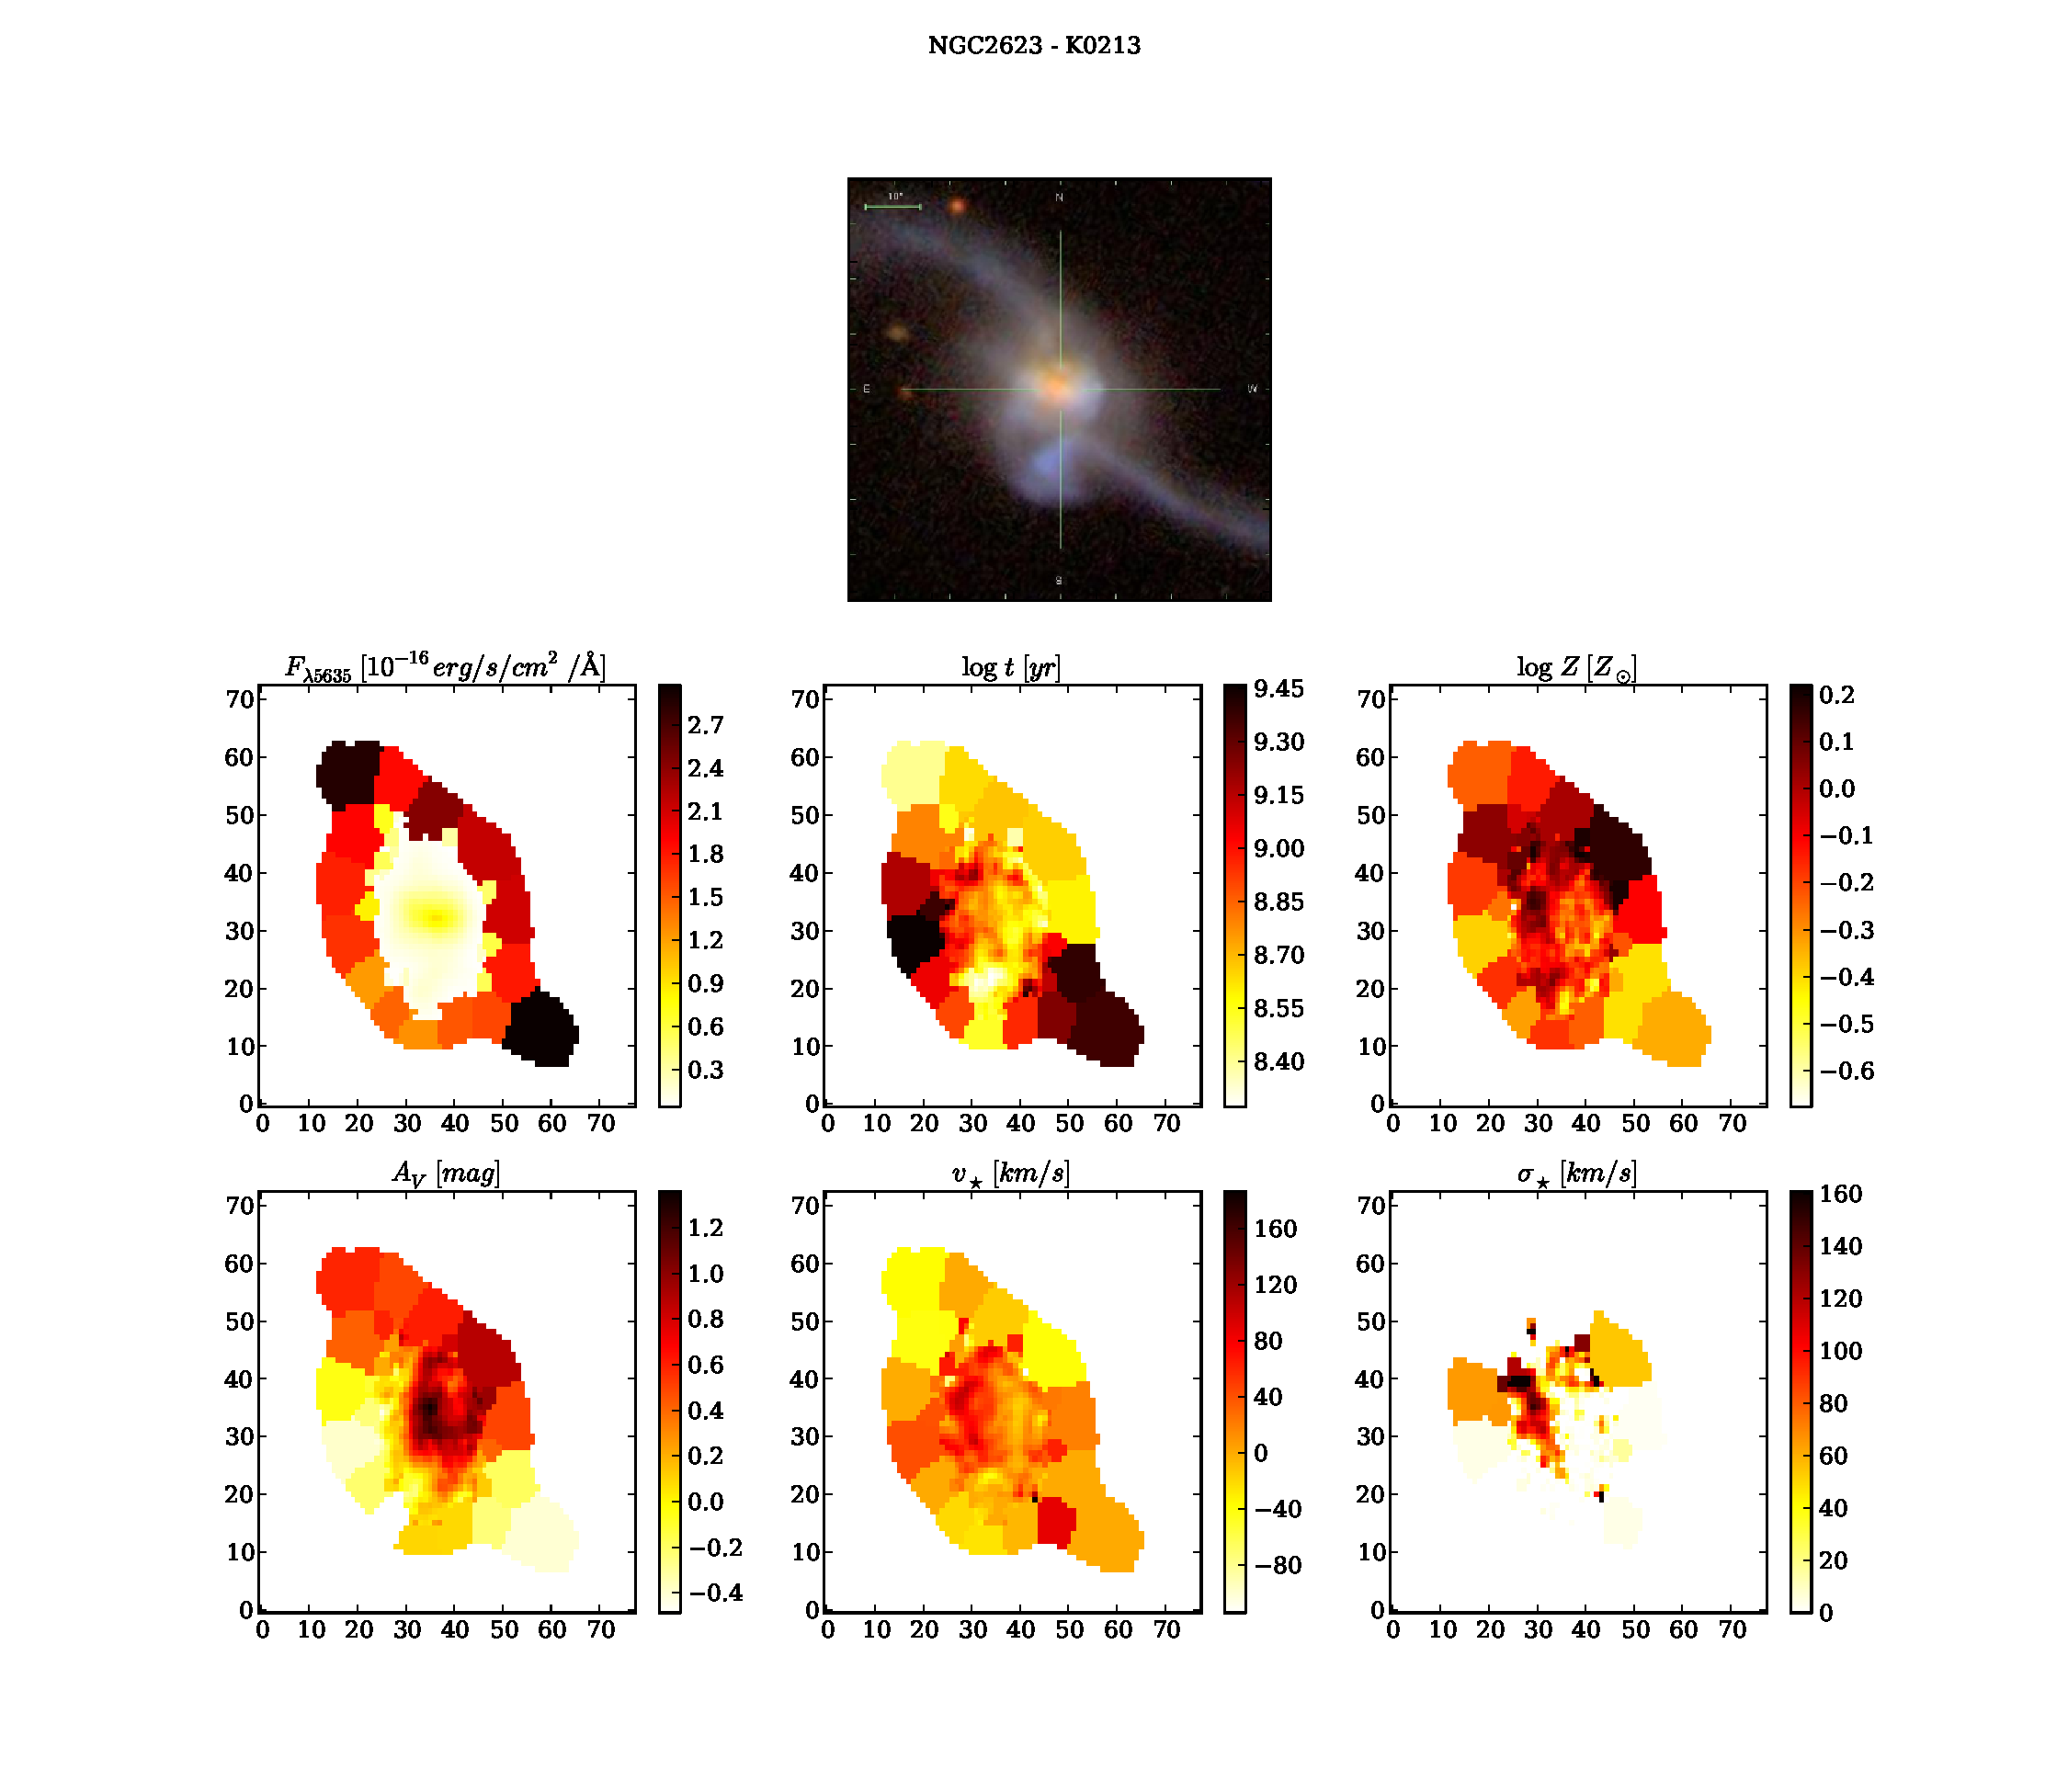
\includegraphics[width=1.\textwidth]{figuras/K0213-apresent.pdf}
    \caption[Propriedades f\'isicas da gal\'axia NGC 2623.]
    {Igual a Figura \ref{fig:K0008apresent} para a galáxia NGC 2623.}
    \label{fig:K0213apresent}
\end{figure}

\begin{figure}
    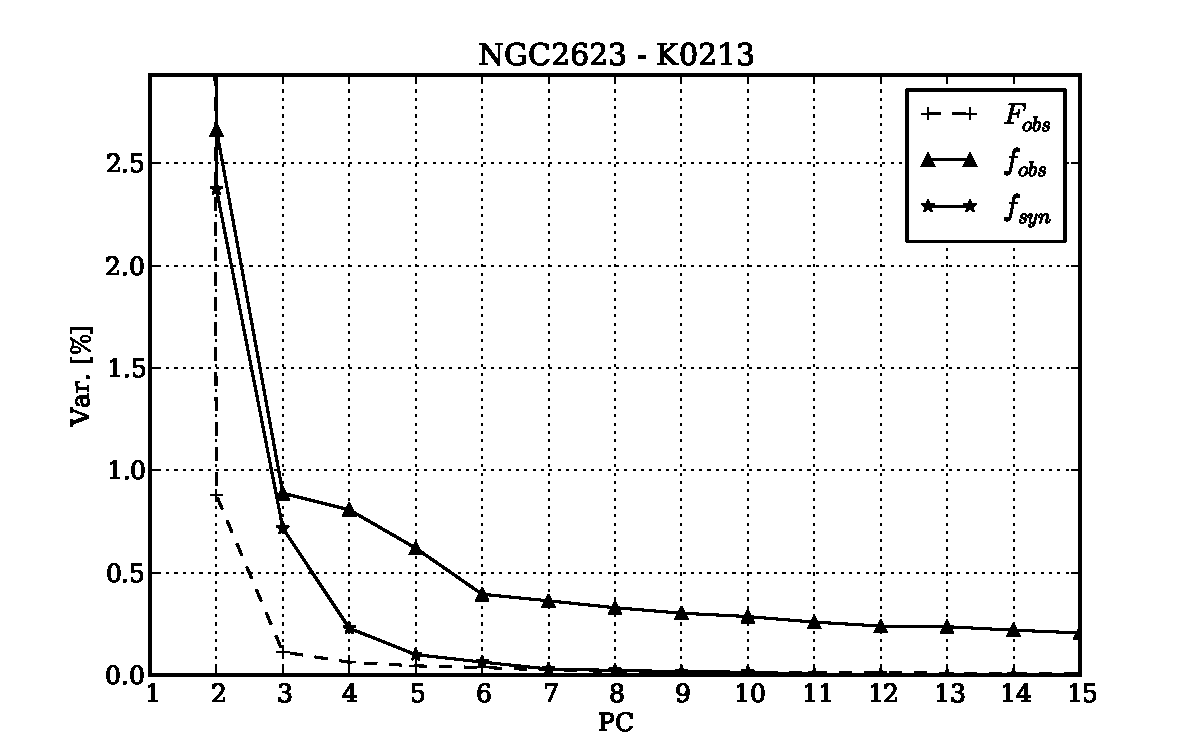
\includegraphics[height=0.33\textheight]{figuras/K0213-screetest.pdf}
    \caption[Scree test comparativo entre 3 PCAs - NGC 2623.]
    {Igual a Figura \ref{fig:K0008scree} para a galáxia NGC 2623.}
    \label{fig:K0213scree}
\end{figure}

\begin{figure}
    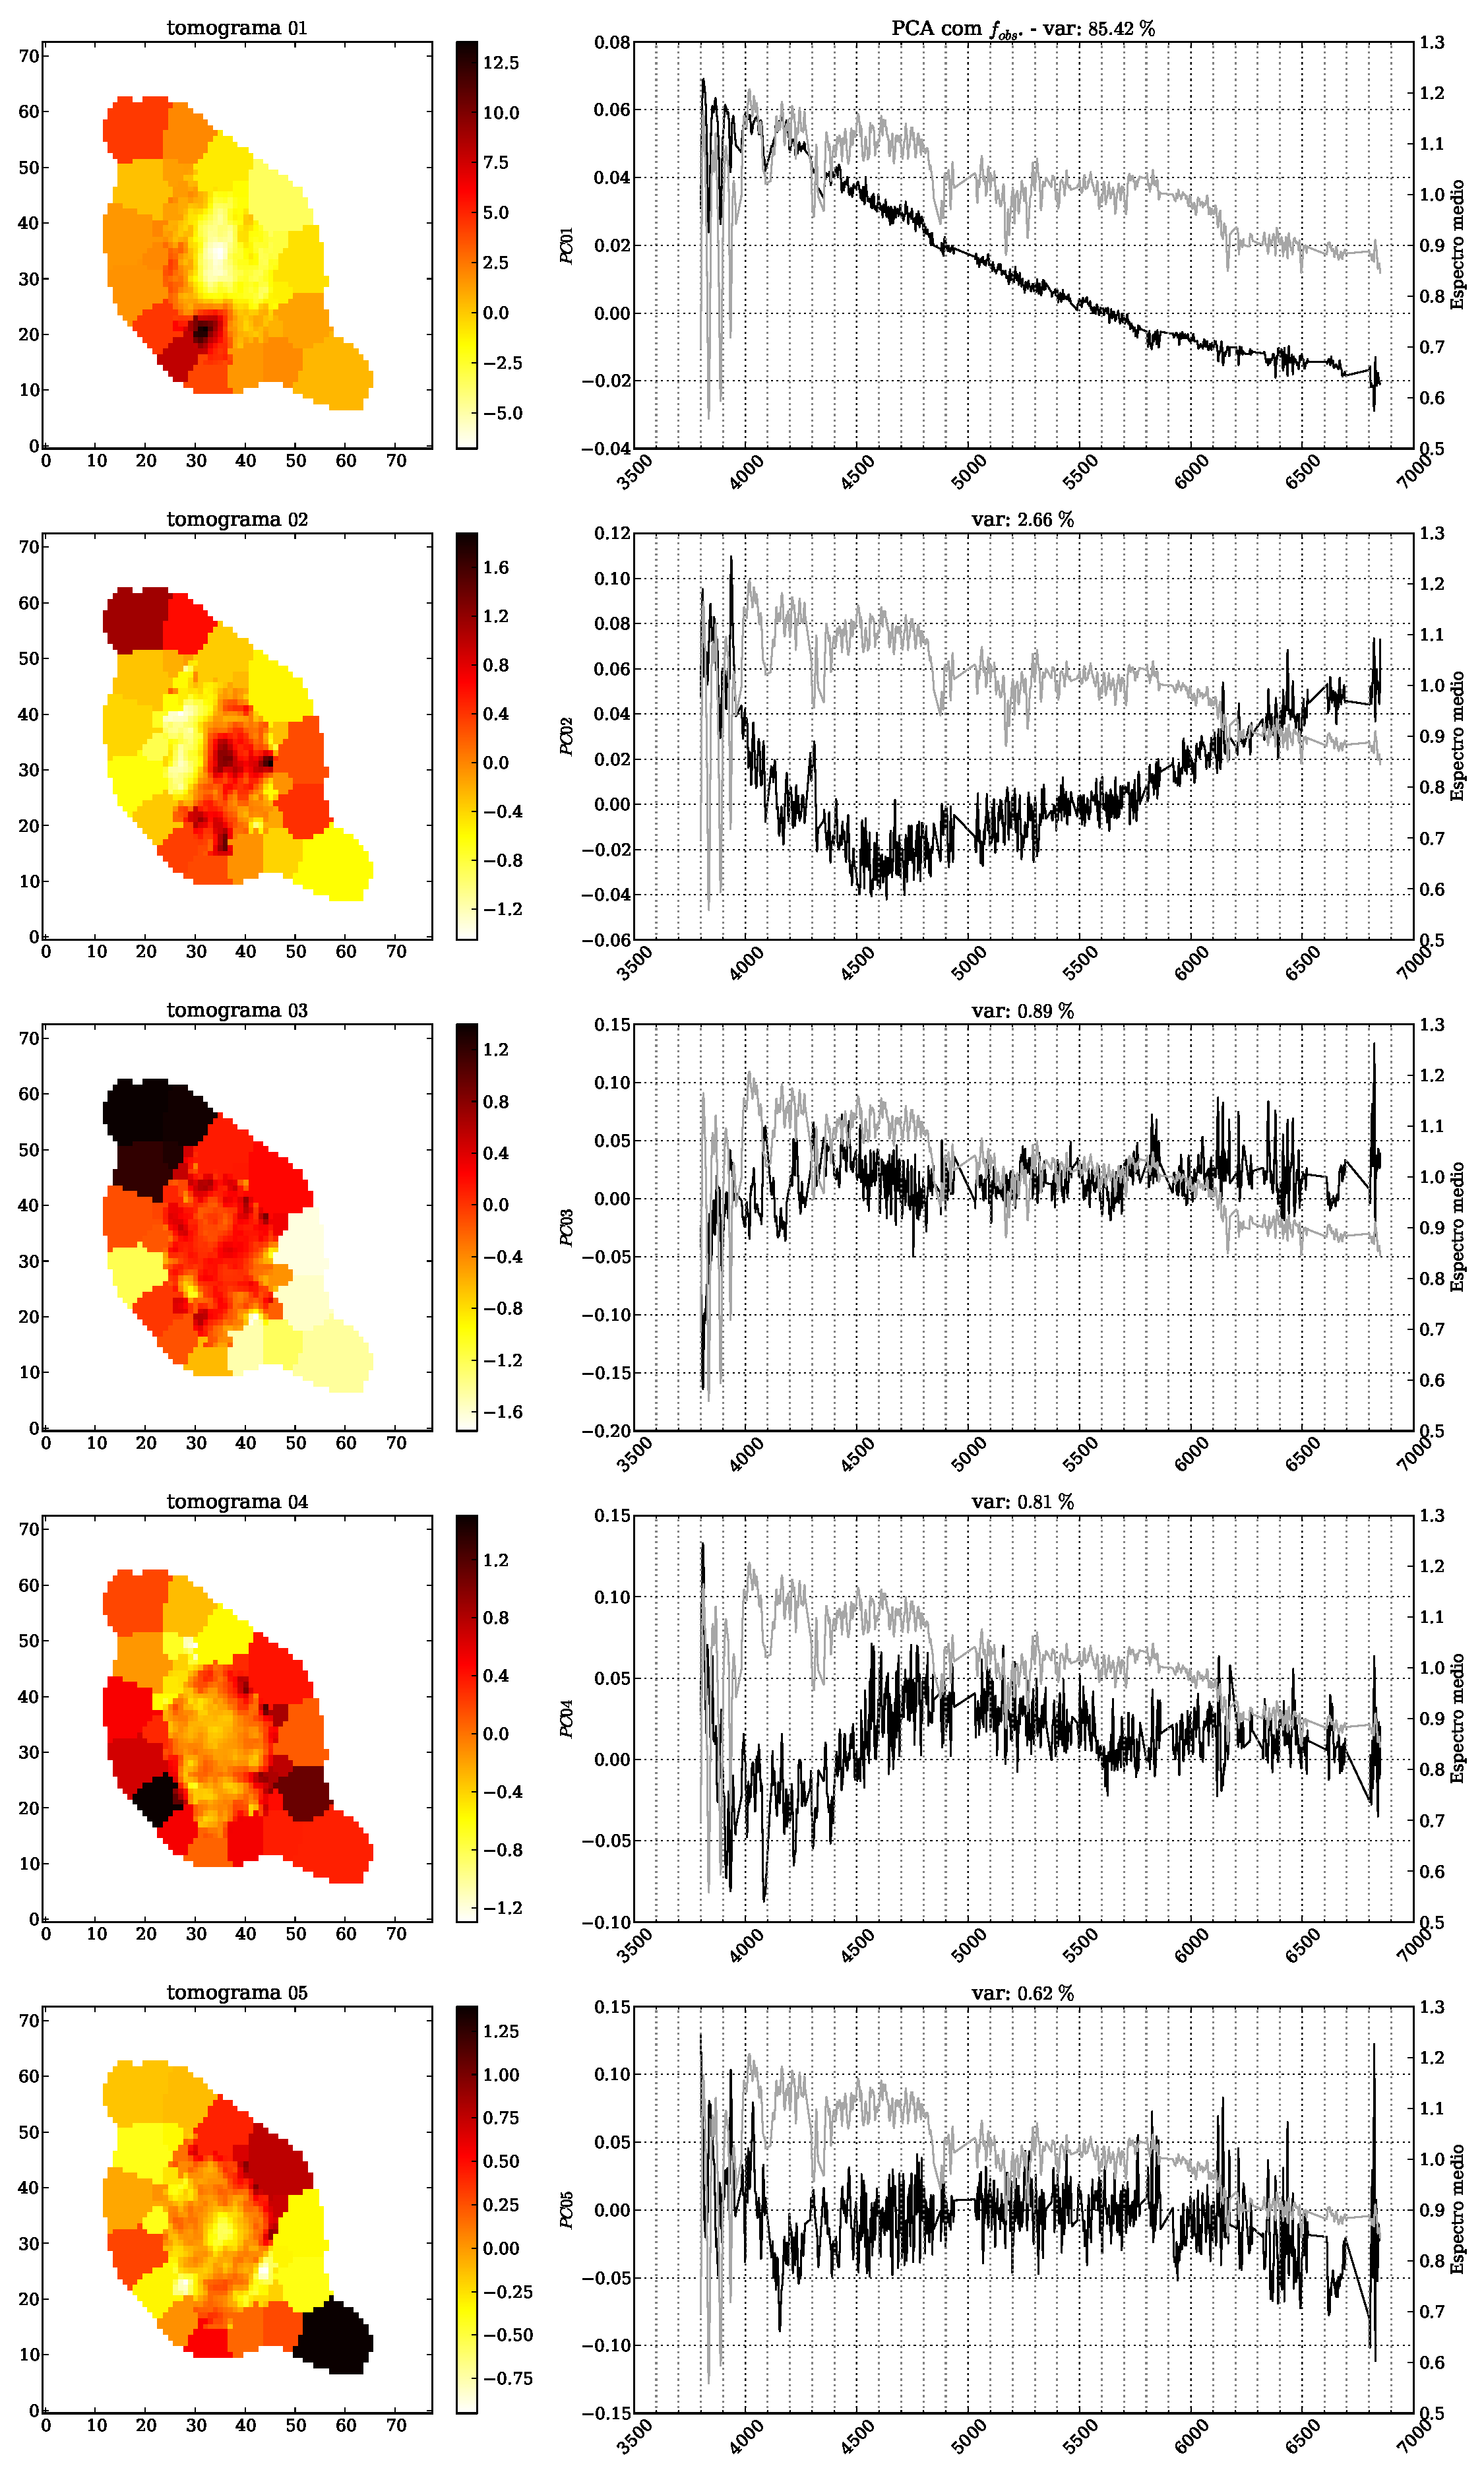
\includegraphics[width=0.8\textwidth]{figuras/K0213-tomo-obs-norm.pdf}
    \caption[Tomogramas de 1 a 5 para o cubo $f_{obs}$ - NGC 2623.]
    {Igual a Figura \ref{fig:K0008tomofobsnorm} para a galáxia NGC 2623.}
    \label{fig:K0213tomofobsnorm}
\end{figure}

\begin{figure}
    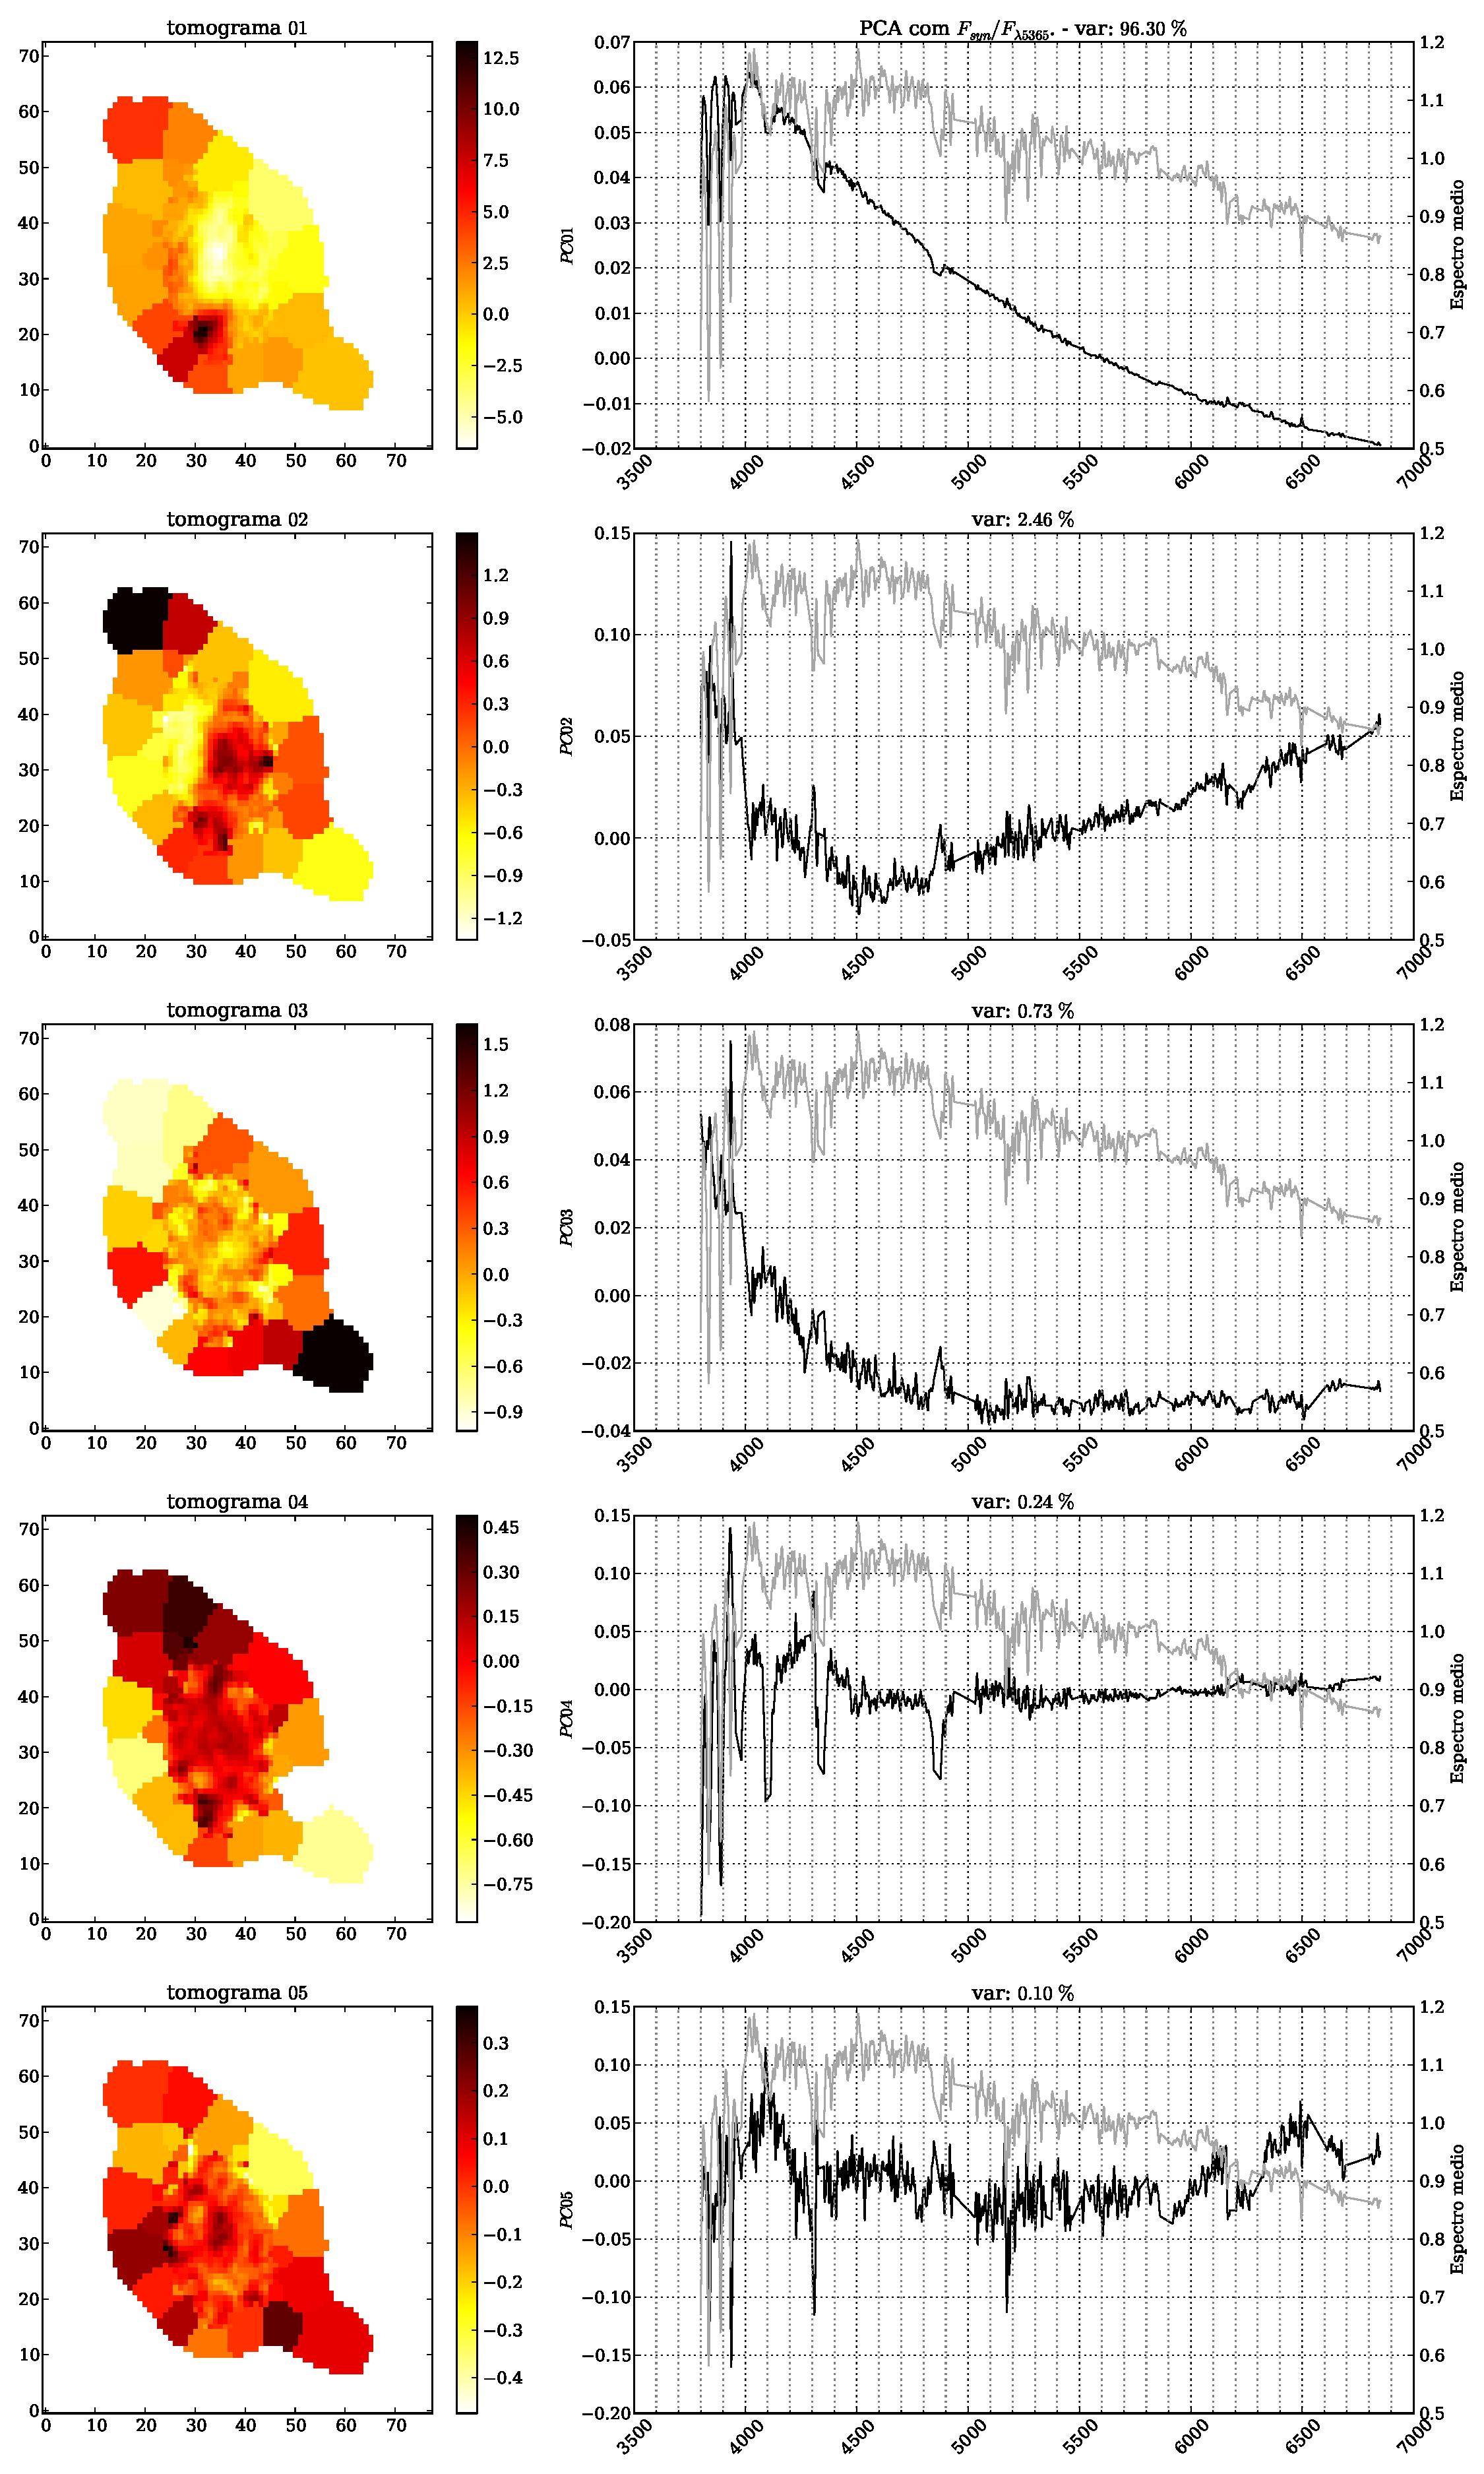
\includegraphics[width=0.8\textwidth]{figuras/K0213-tomo-syn-norm.pdf}
    \caption[Tomogramas de 1 a 5 para o cubo $f_{syn}$ - NGC 2623.]
    {Igual a Figura \ref{fig:K0008tomofsynnorm} para a galáxia NGC 2623.}
    \label{fig:K0213tomofsynnorm}
\end{figure}

\begin{figure}
    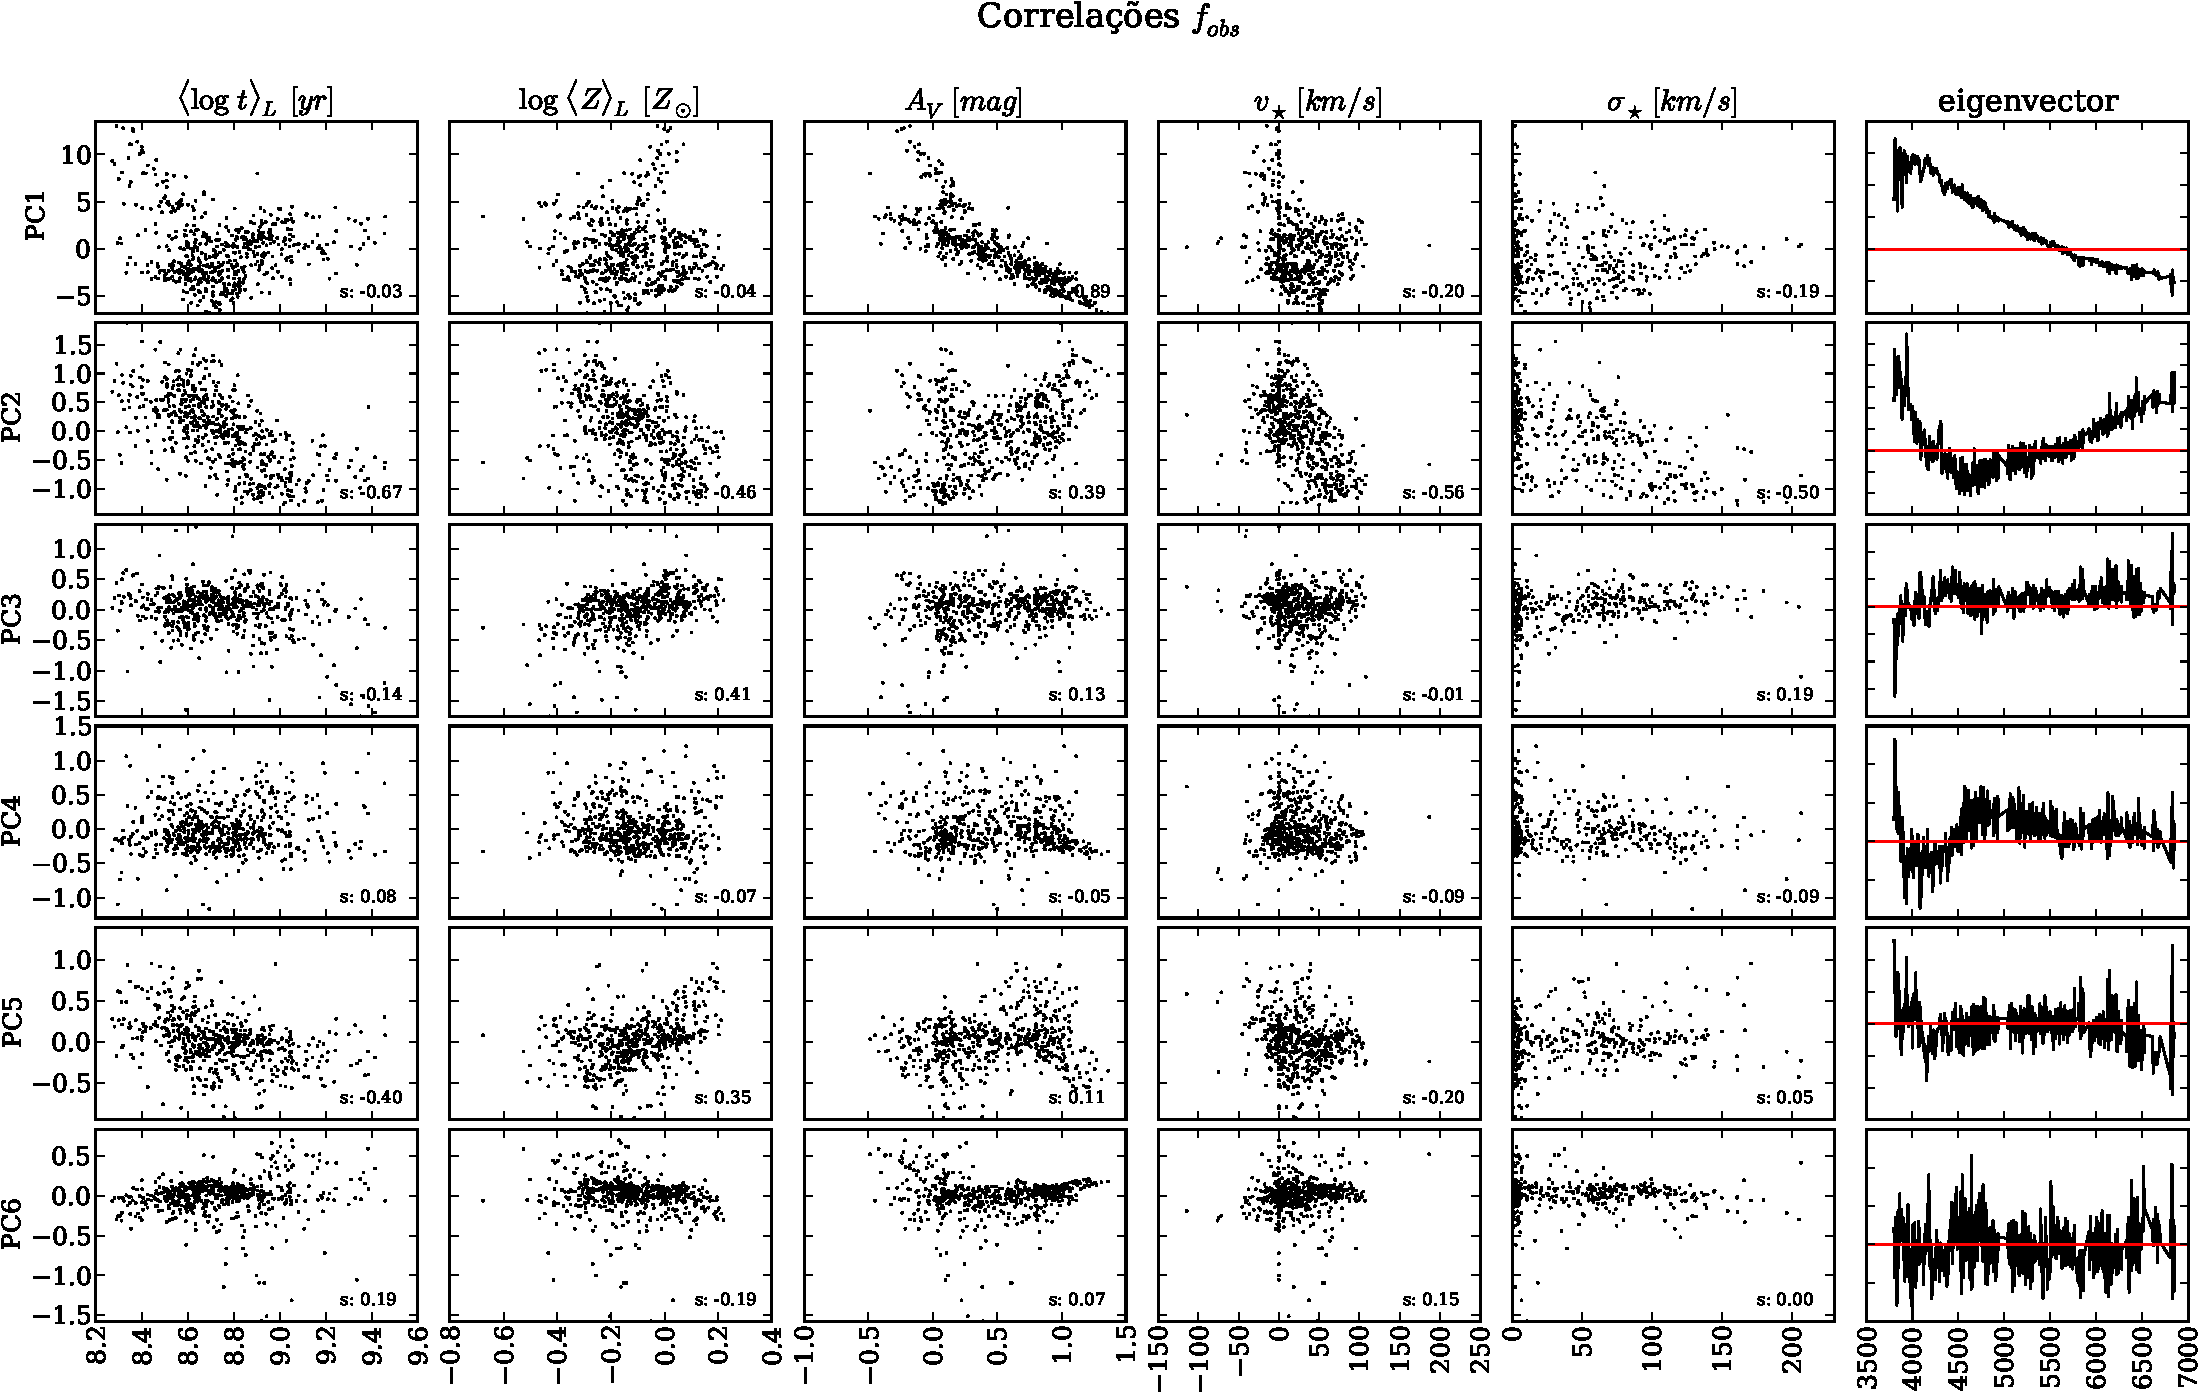
\includegraphics[width=1.2\textwidth, angle=-90]{figuras/K0213-correl-f_obs_norm-PCvsPhys.pdf}
	\caption[Correlações PCs vs. par\^ametros f\'isicos - $f_{obs}$ - NGC 2623.]
	{Igual a Figura \ref{fig:K0008correfobsnorm} para a galáxia NGC 2623.}
    \label{fig:K0213correfobsnorm}
\end{figure}

\begin{figure}
    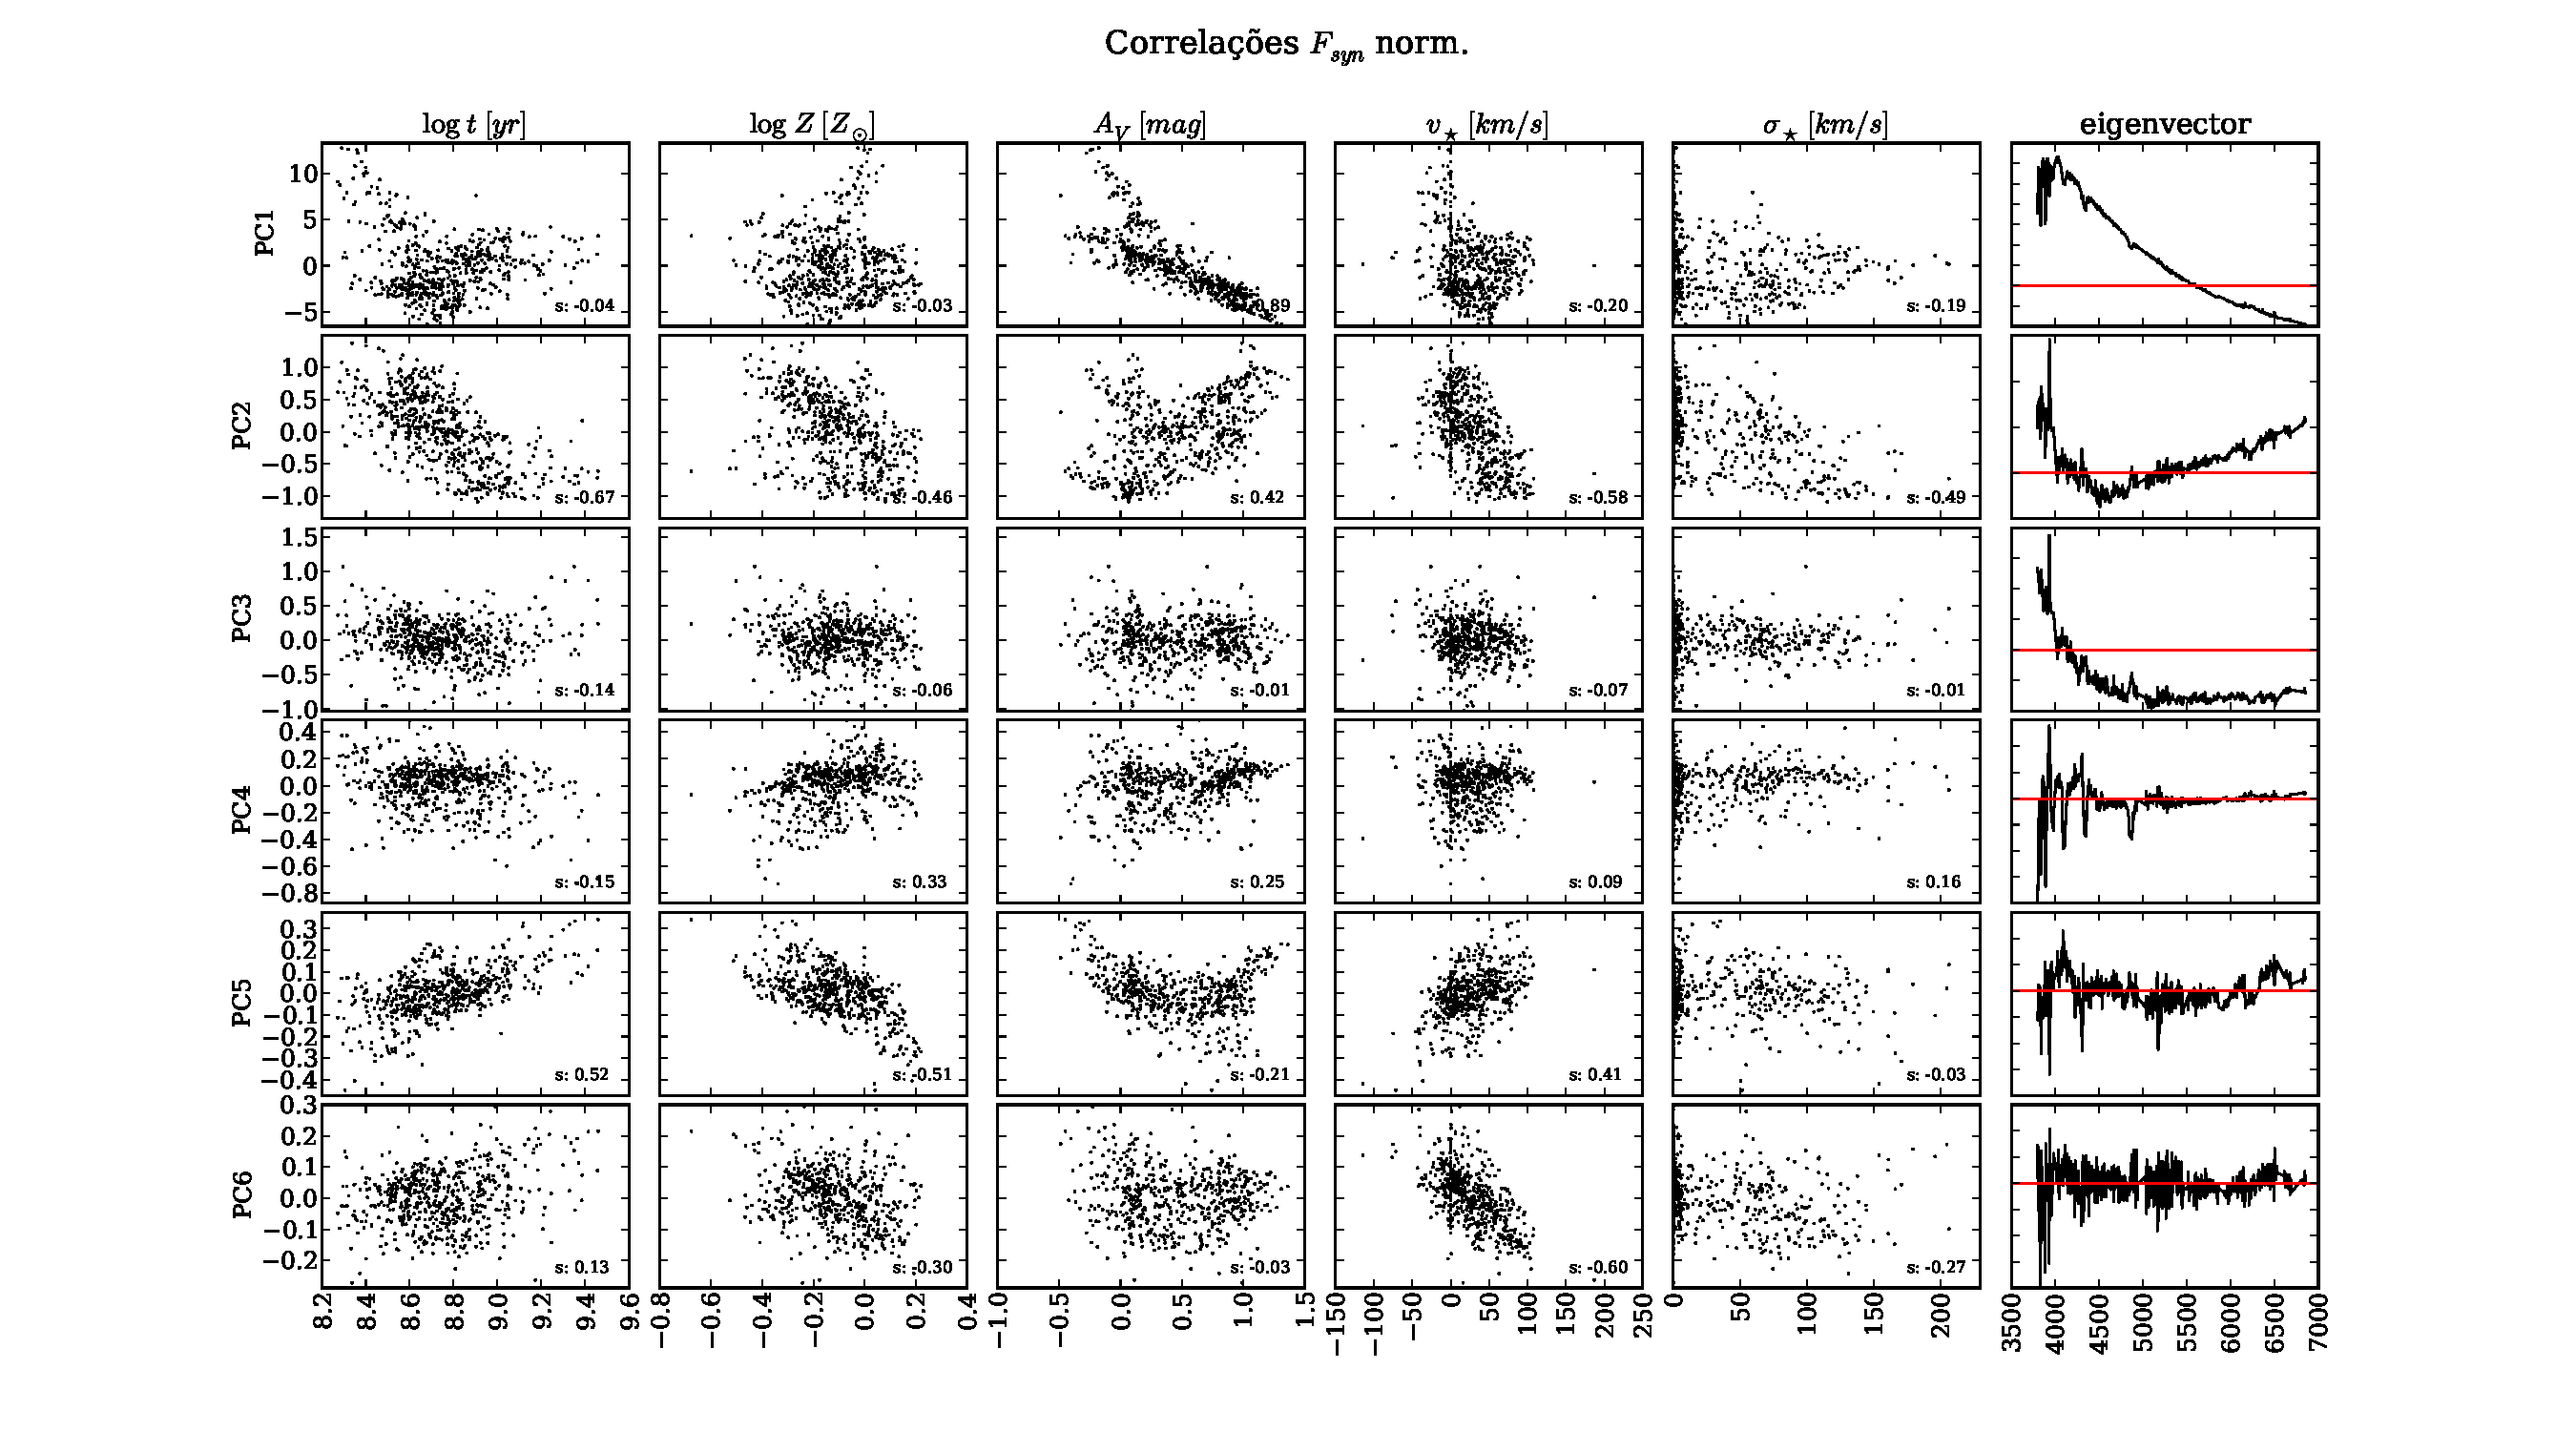
\includegraphics[width=1.2\textwidth, angle=-90]{figuras/K0213-correl-f_syn_norm-PCvsPhys.pdf}
	\caption[Correlações PCs vs. par\^ametros f\'isicos - $f_{syn}$ - NGC 2623.]
	{Igual a Figura \ref{fig:K0008correfsynnorm} para a galáxia NGC 2623.}
    \label{fig:K0213correfsynnorm}
\end{figure}

\subsection{ARP 220 - CALIFA 802}

Esse objeto peculiar é a ULIRG ({\em Ultraluminous infrared galaxy}) mais próxima da Terra. Como a NGC 2623, possui uma
densa núvem de poeira no centro (Figura \ref{fig:K0802apresent}). Repete o mesmo comportamento assintótico de todos os
{\em scree tests} (Figura \ref{fig:K0802scree}) anteriores e possui $\sim 99\%$ da variância contida nas primeiras 5 PCs
para o caso observado ($\sim 99.7\%$ para o caso sintético).

Também como a NGC 2623, possui as duas primeiras PCs muito semelhantes (Figuras \ref{fig:K0802tomofobsnorm} e
\ref{fig:K0802tomofsynnorm}). Comparando as correlações (Figuras \ref{fig:K0802correfobsnorm} e
\ref{fig:K0802correfsynnorm}) vemos que a primeira PC correlaciona fortemente com $A_V$ e de maneira mais fraca com a
idade. A segunda, apesar de ter uma leve correlação com todos as propriedades, a metalicidade se ressalta em ambos os
casos. Para o caso observado a PC3 correlaciona melhor com a velocidade estelar. No caso sintético vemos vestígios da
sequência de Balmer tanto na PC3 (que não correlaciona fortemente com nada) quanto na PC4 (que parece ser uma boa medida
de $v_\star$). Ainda no caso sintético, vemos que a velocidade aparece fortemente também na PC5, mas divide espaço (em
correlação) com idade e metalicidade de maneira mais fraca. Já para o caso observado nenhuma delas (PC4, PC5) paracem
ter correlação com nenhum dos parâmetros físicos comparados. O mesmo para a PC6 em ambos os casos.

\begin{figure}
    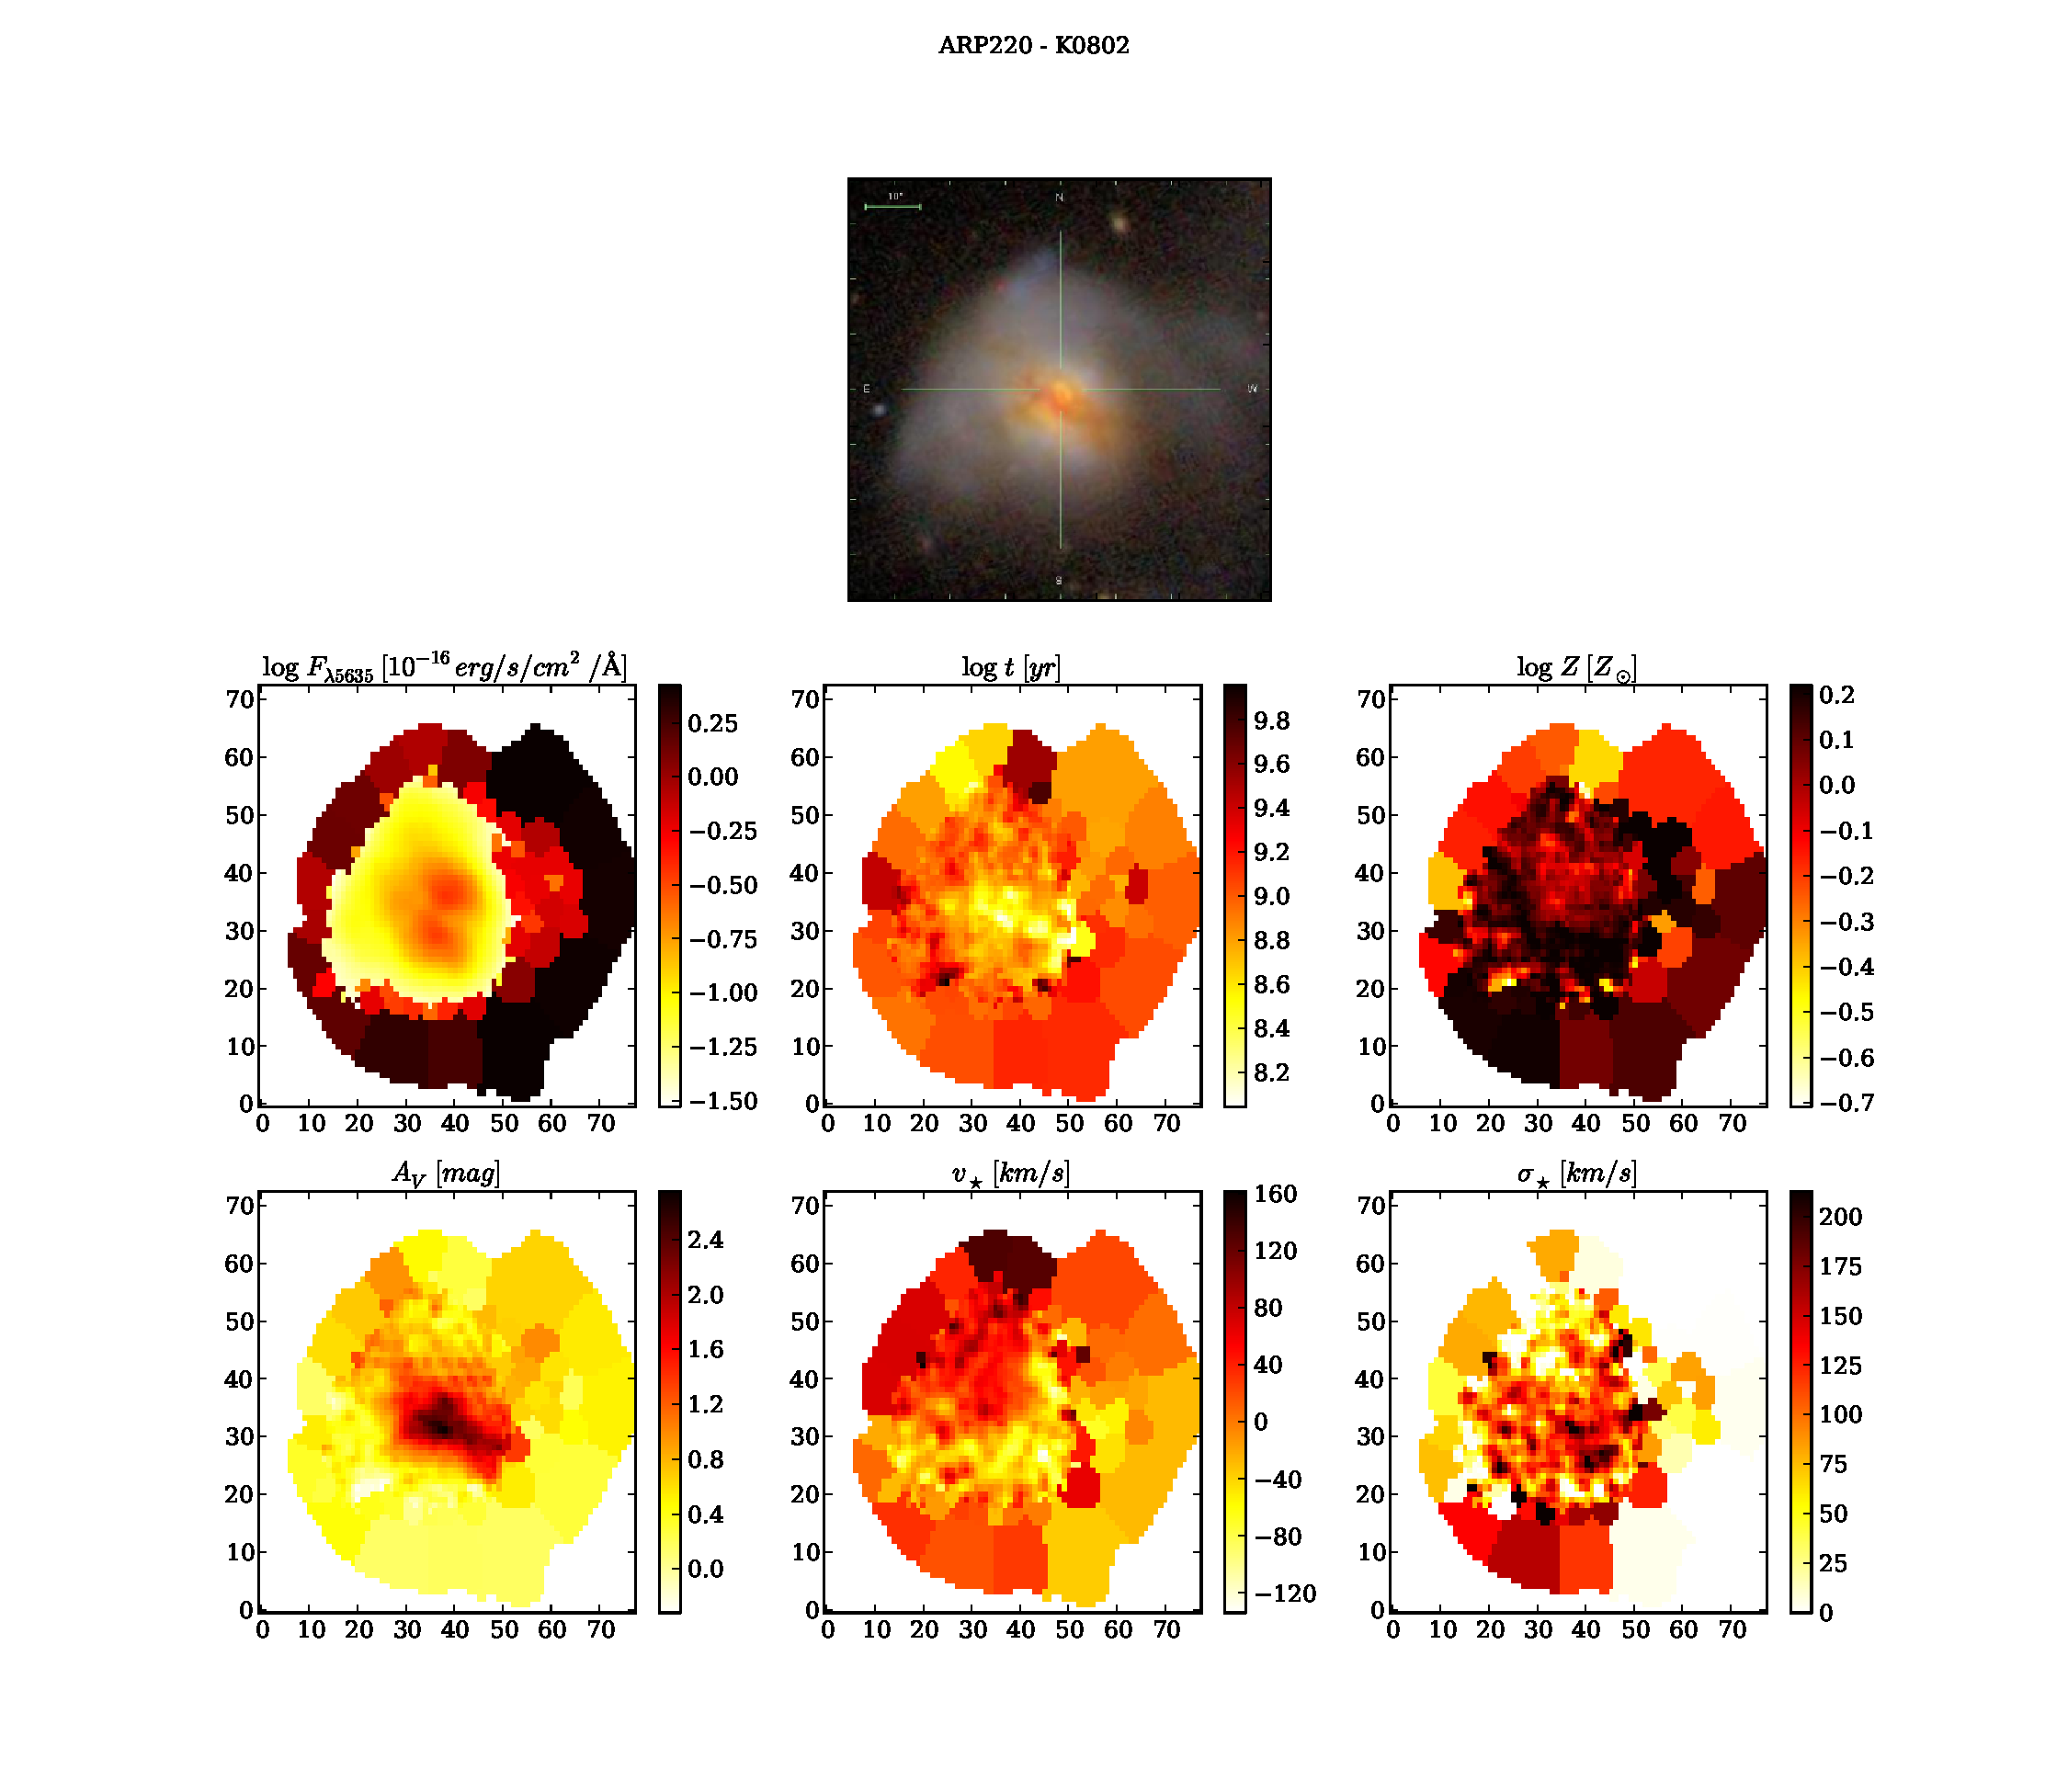
\includegraphics[width=1.\textwidth]{figuras/K0802-apresent.pdf}
    \caption[Propriedades f\'isicas da gal\'axia ARP 220.]
    {Igual a Figura \ref{fig:K0008apresent} para a galáxia ARP 220.}
    \label{fig:K0802apresent}
\end{figure}

\begin{figure}
    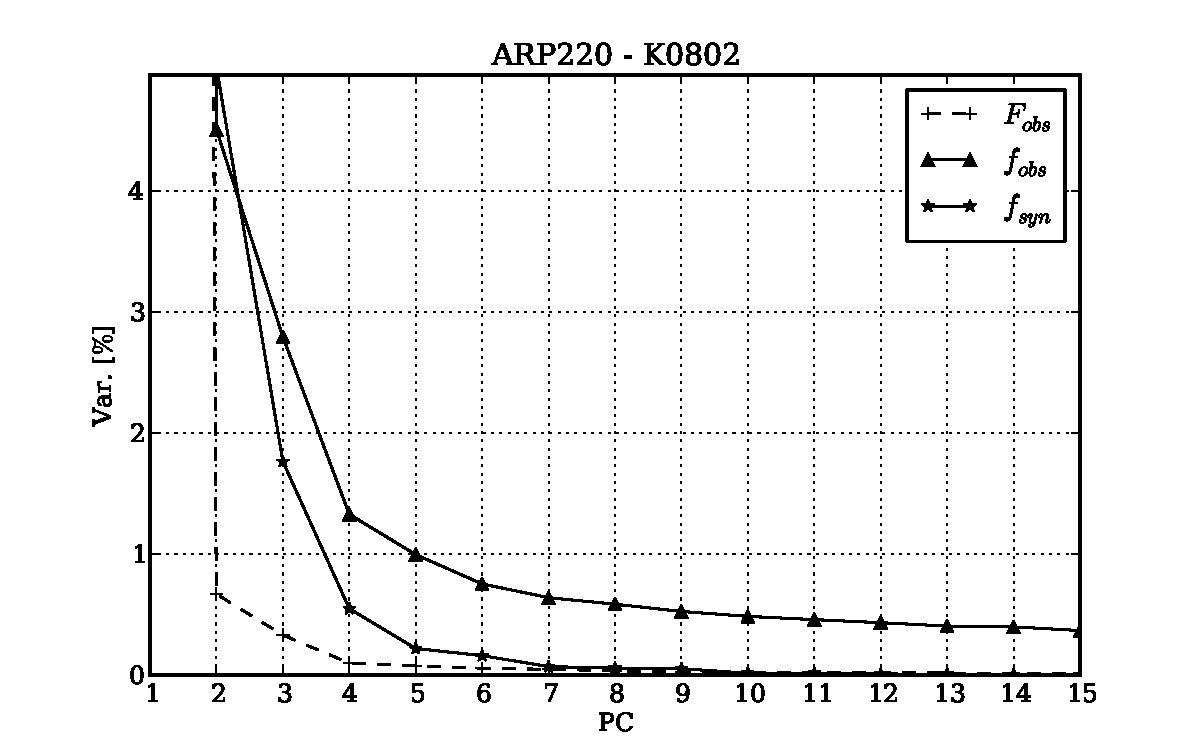
\includegraphics[height=0.33\textheight]{figuras/K0802-screetest.pdf}
    \caption[Scree test comparativo entre 3 PCAs - ARP 220.]
	{Igual a Figura \ref{fig:K0008scree} para a galáxia ARP 220.}
    \label{fig:K0802scree}
\end{figure}

\begin{figure}
    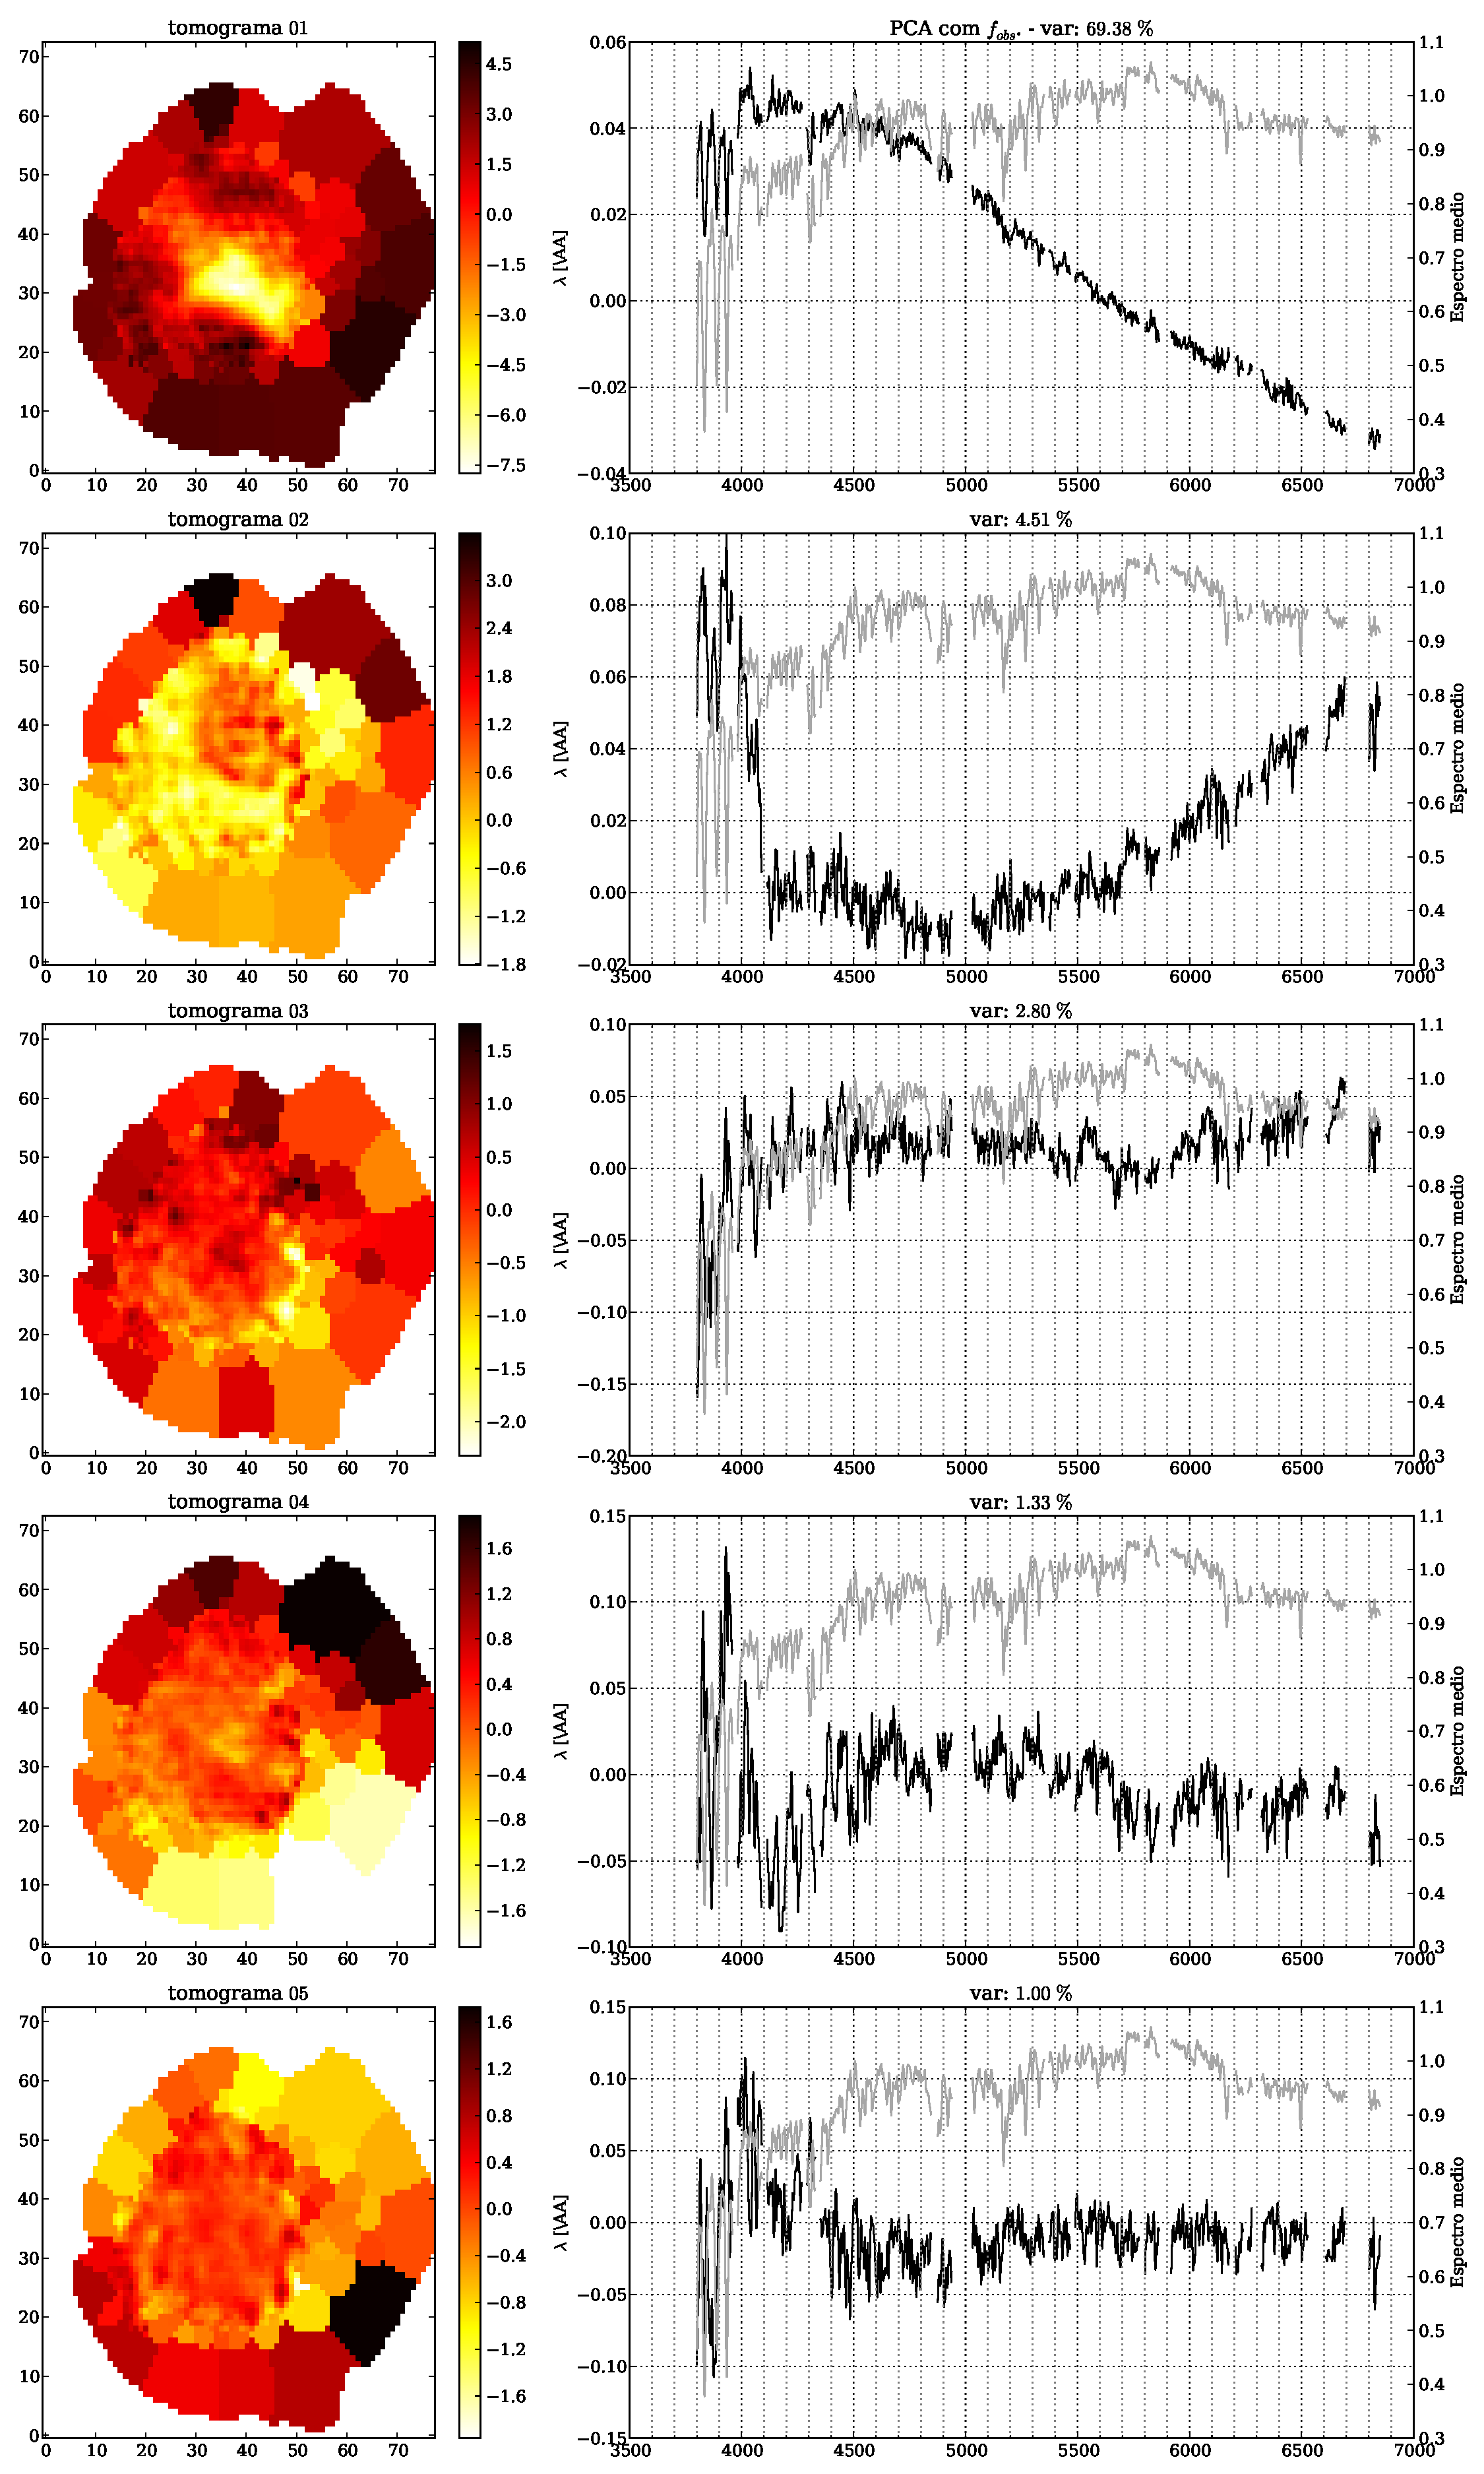
\includegraphics[width=0.8\textwidth]{figuras/K0802-tomo-obs-norm.pdf}
    \caption[Tomogramas de 1 a 5 para o cubo $f_{obs}$ - ARP 220.]
    {Igual a Figura \ref{fig:K0008tomofobsnorm} para a galáxia ARP 220.}
    \label{fig:K0802tomofobsnorm}
\end{figure}

\begin{figure}
    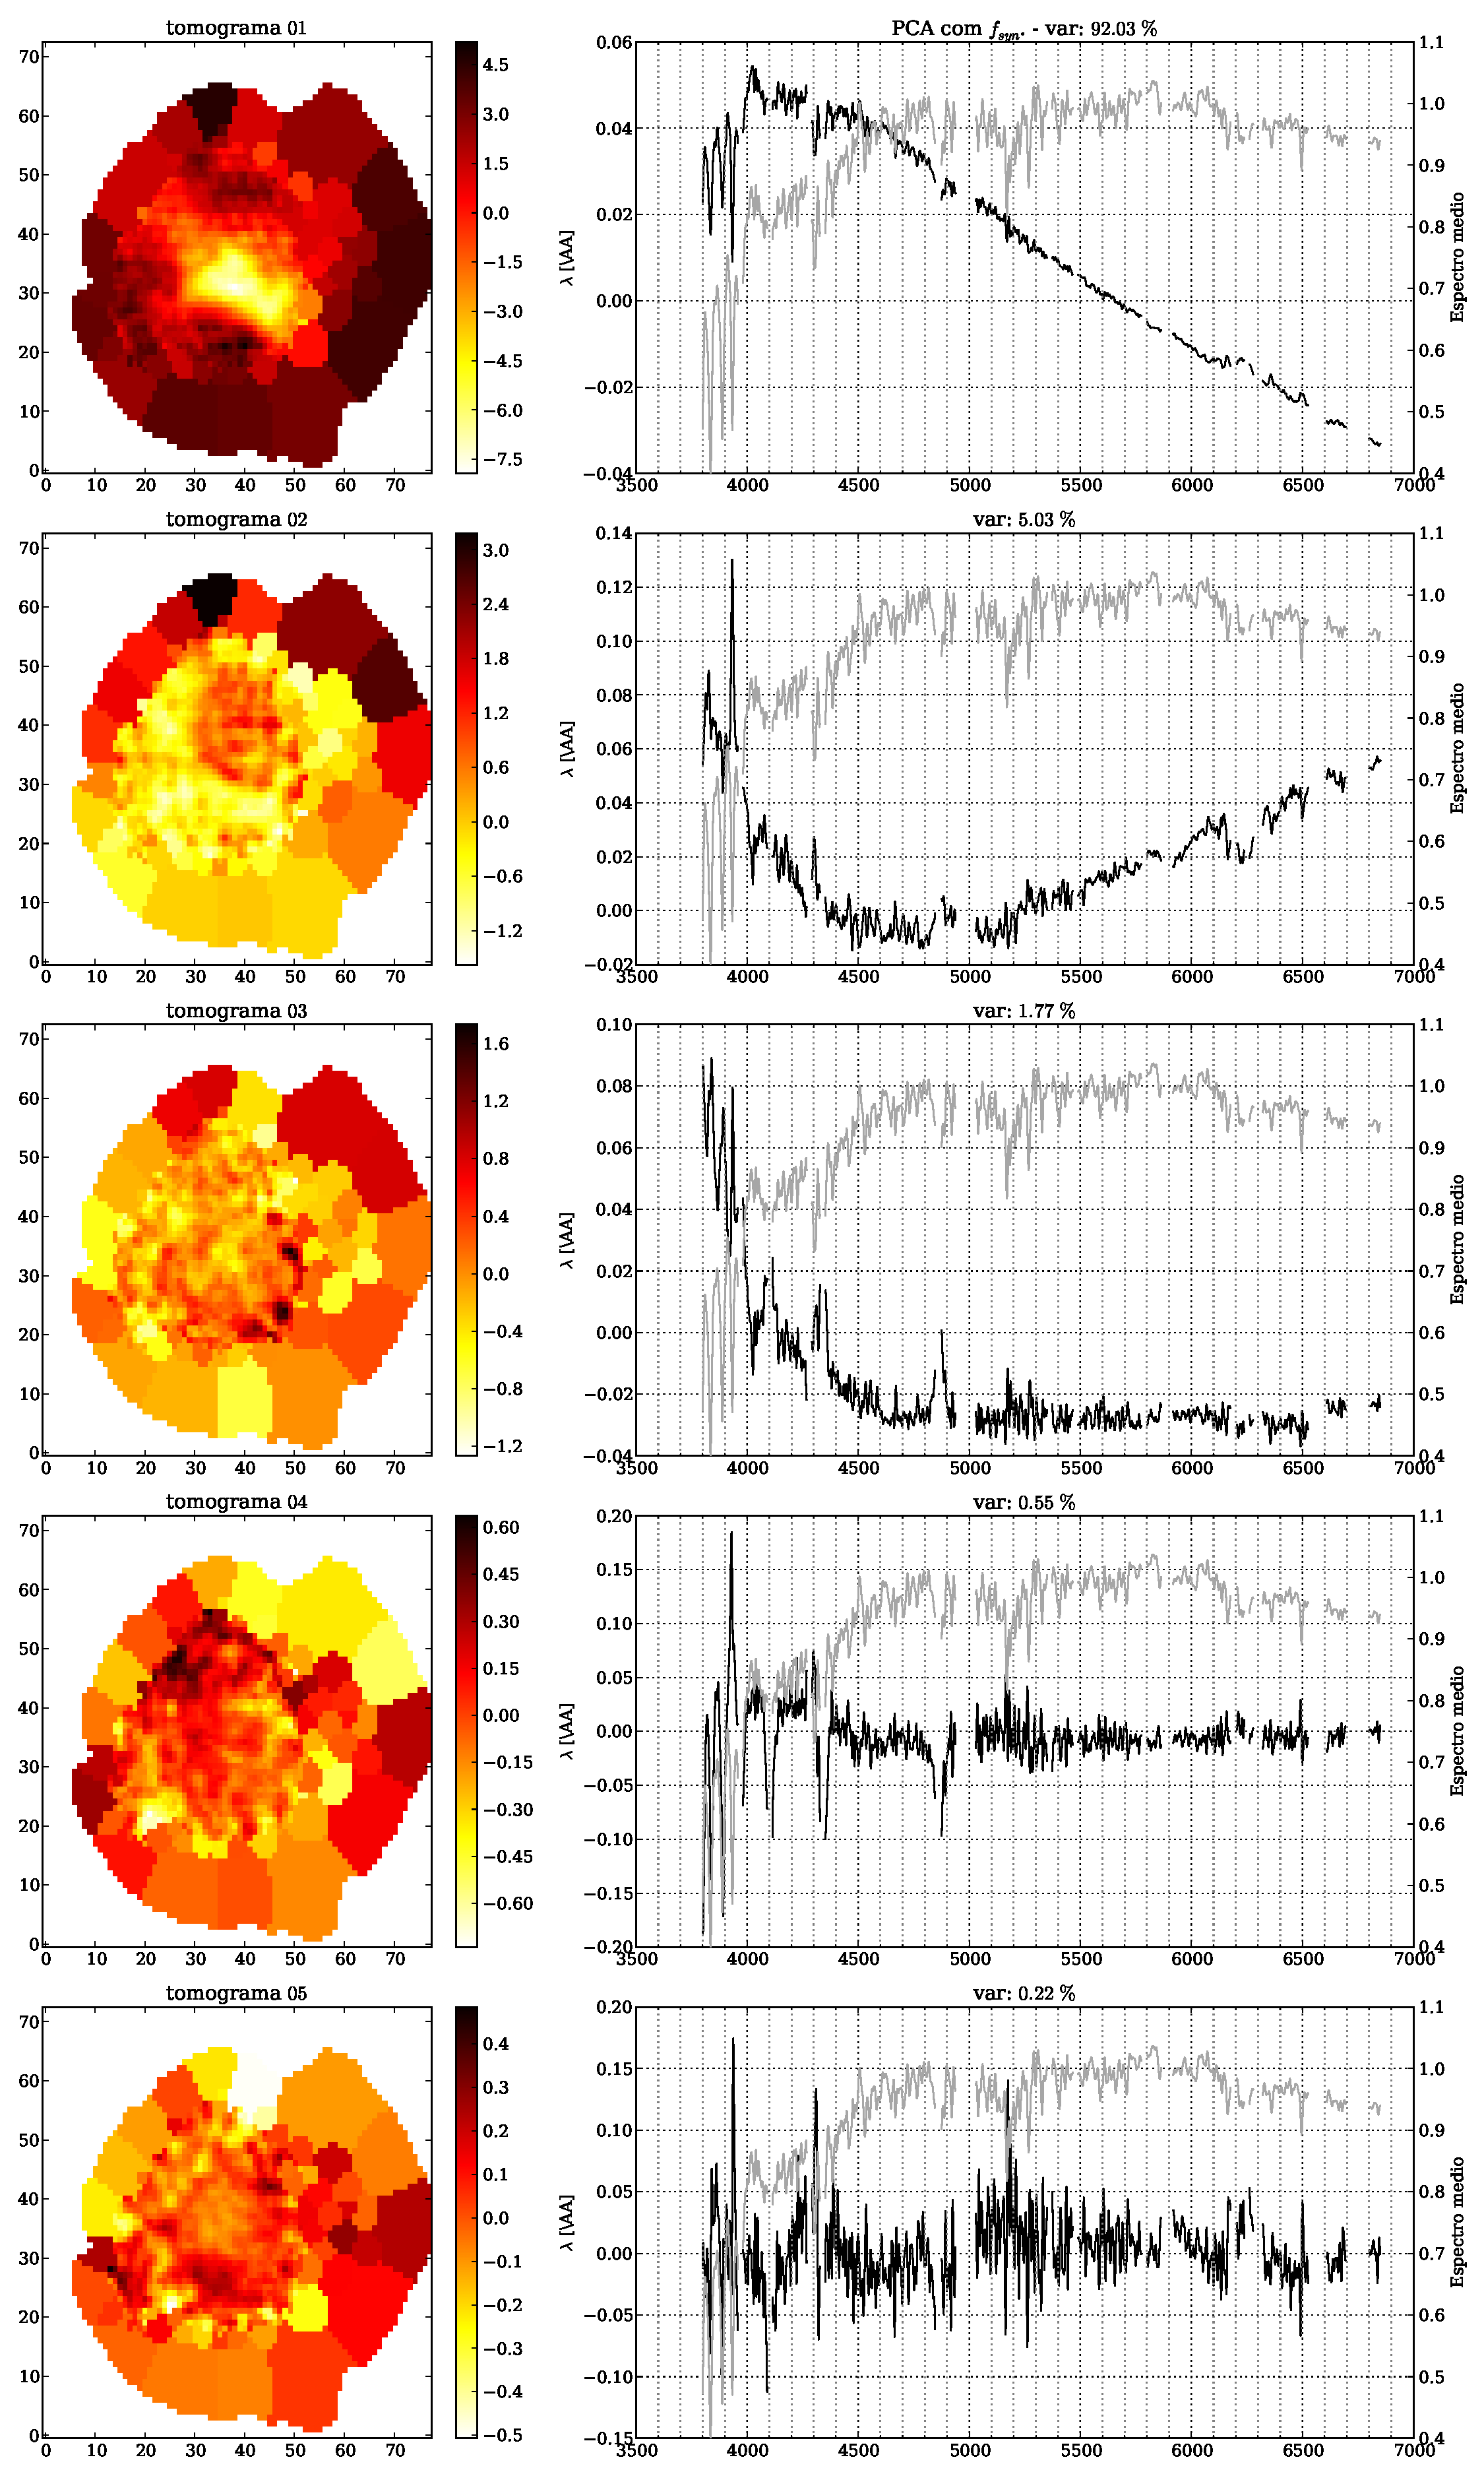
\includegraphics[width=0.8\textwidth]{figuras/K0802-tomo-syn-norm.pdf}
    \caption[Tomogramas de 1 a 5 para o cubo $f_{obs}$ - ARP 220.]
    {Igual a Figura \ref{fig:K0008tomofsynnorm} para a galáxia ARP 220.}
    \label{fig:K0802tomofsynnorm}
\end{figure}

\begin{figure}
    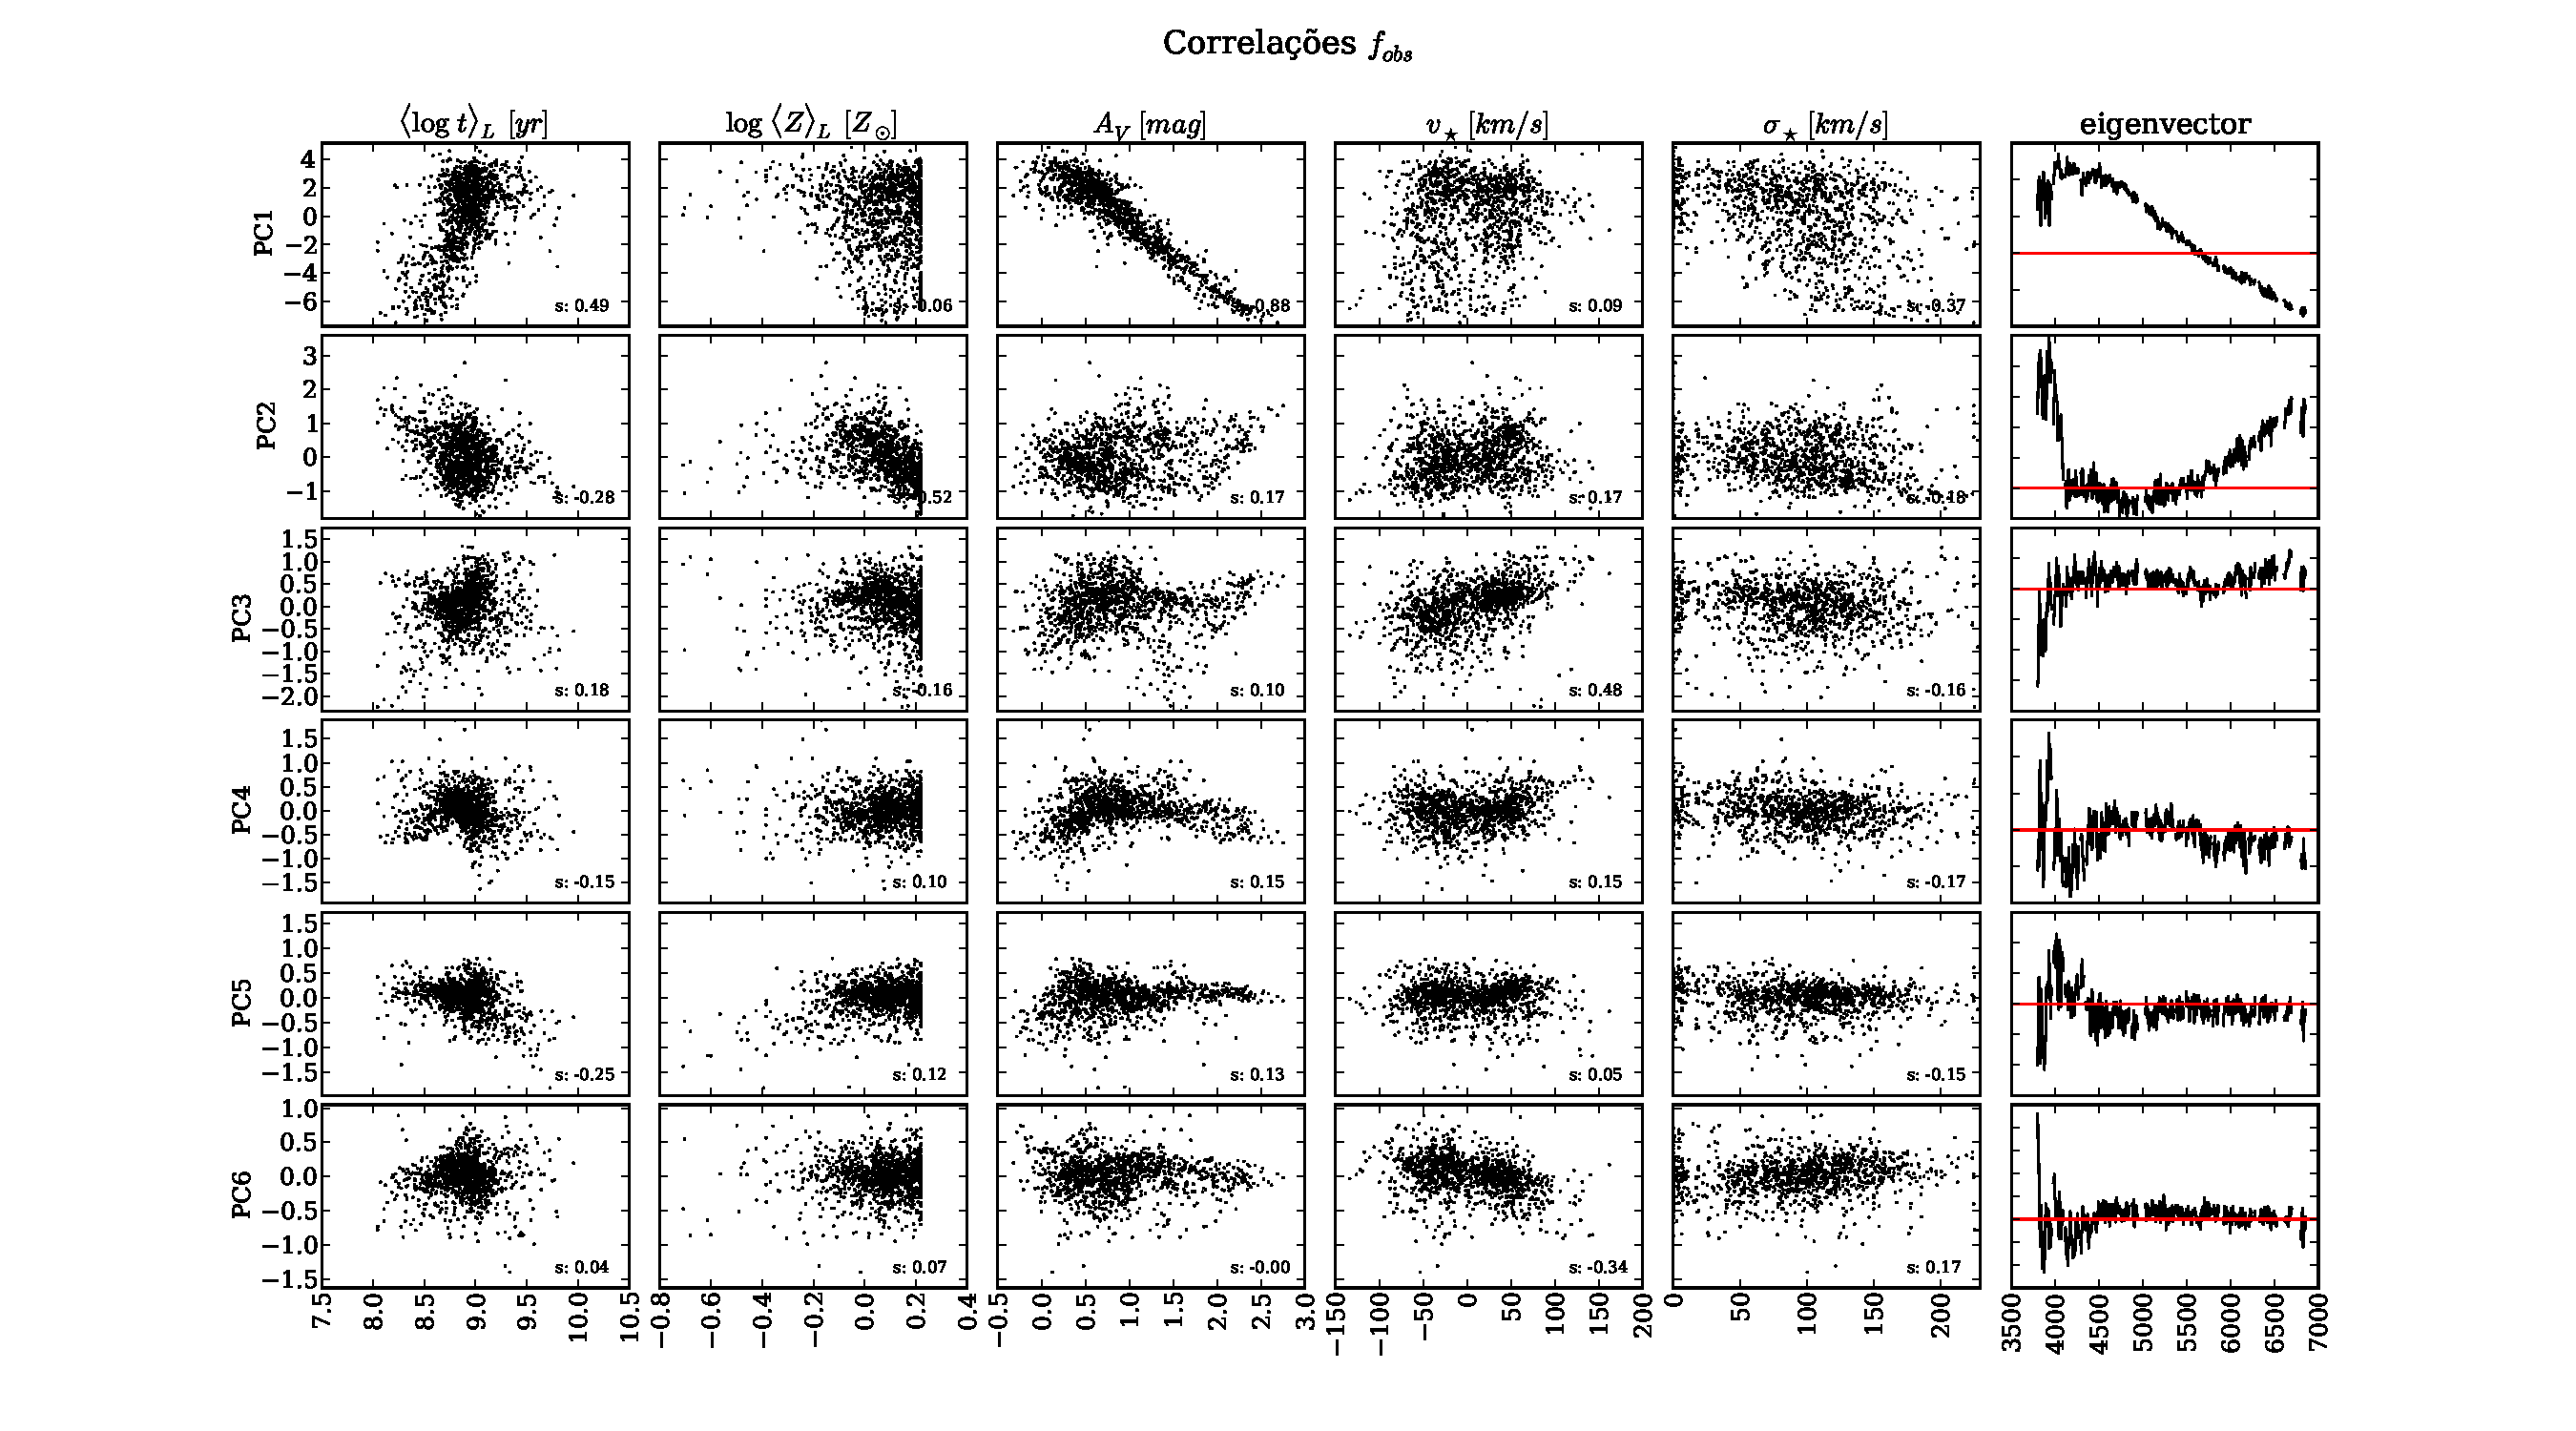
\includegraphics[width=1.2\textwidth, angle=-90]{figuras/K0802-correl-f_obs_norm-PCvsPhys.pdf}
	\caption[Correlações PCs vs. par\^ametros f\'isicos - $f_{obs}$ - ARP 220.]
	{Igual a Figura \ref{fig:K0008correfobsnorm} para a galáxia ARP 220.}
    \label{fig:K0802correfobsnorm}
\end{figure}

\begin{figure}
    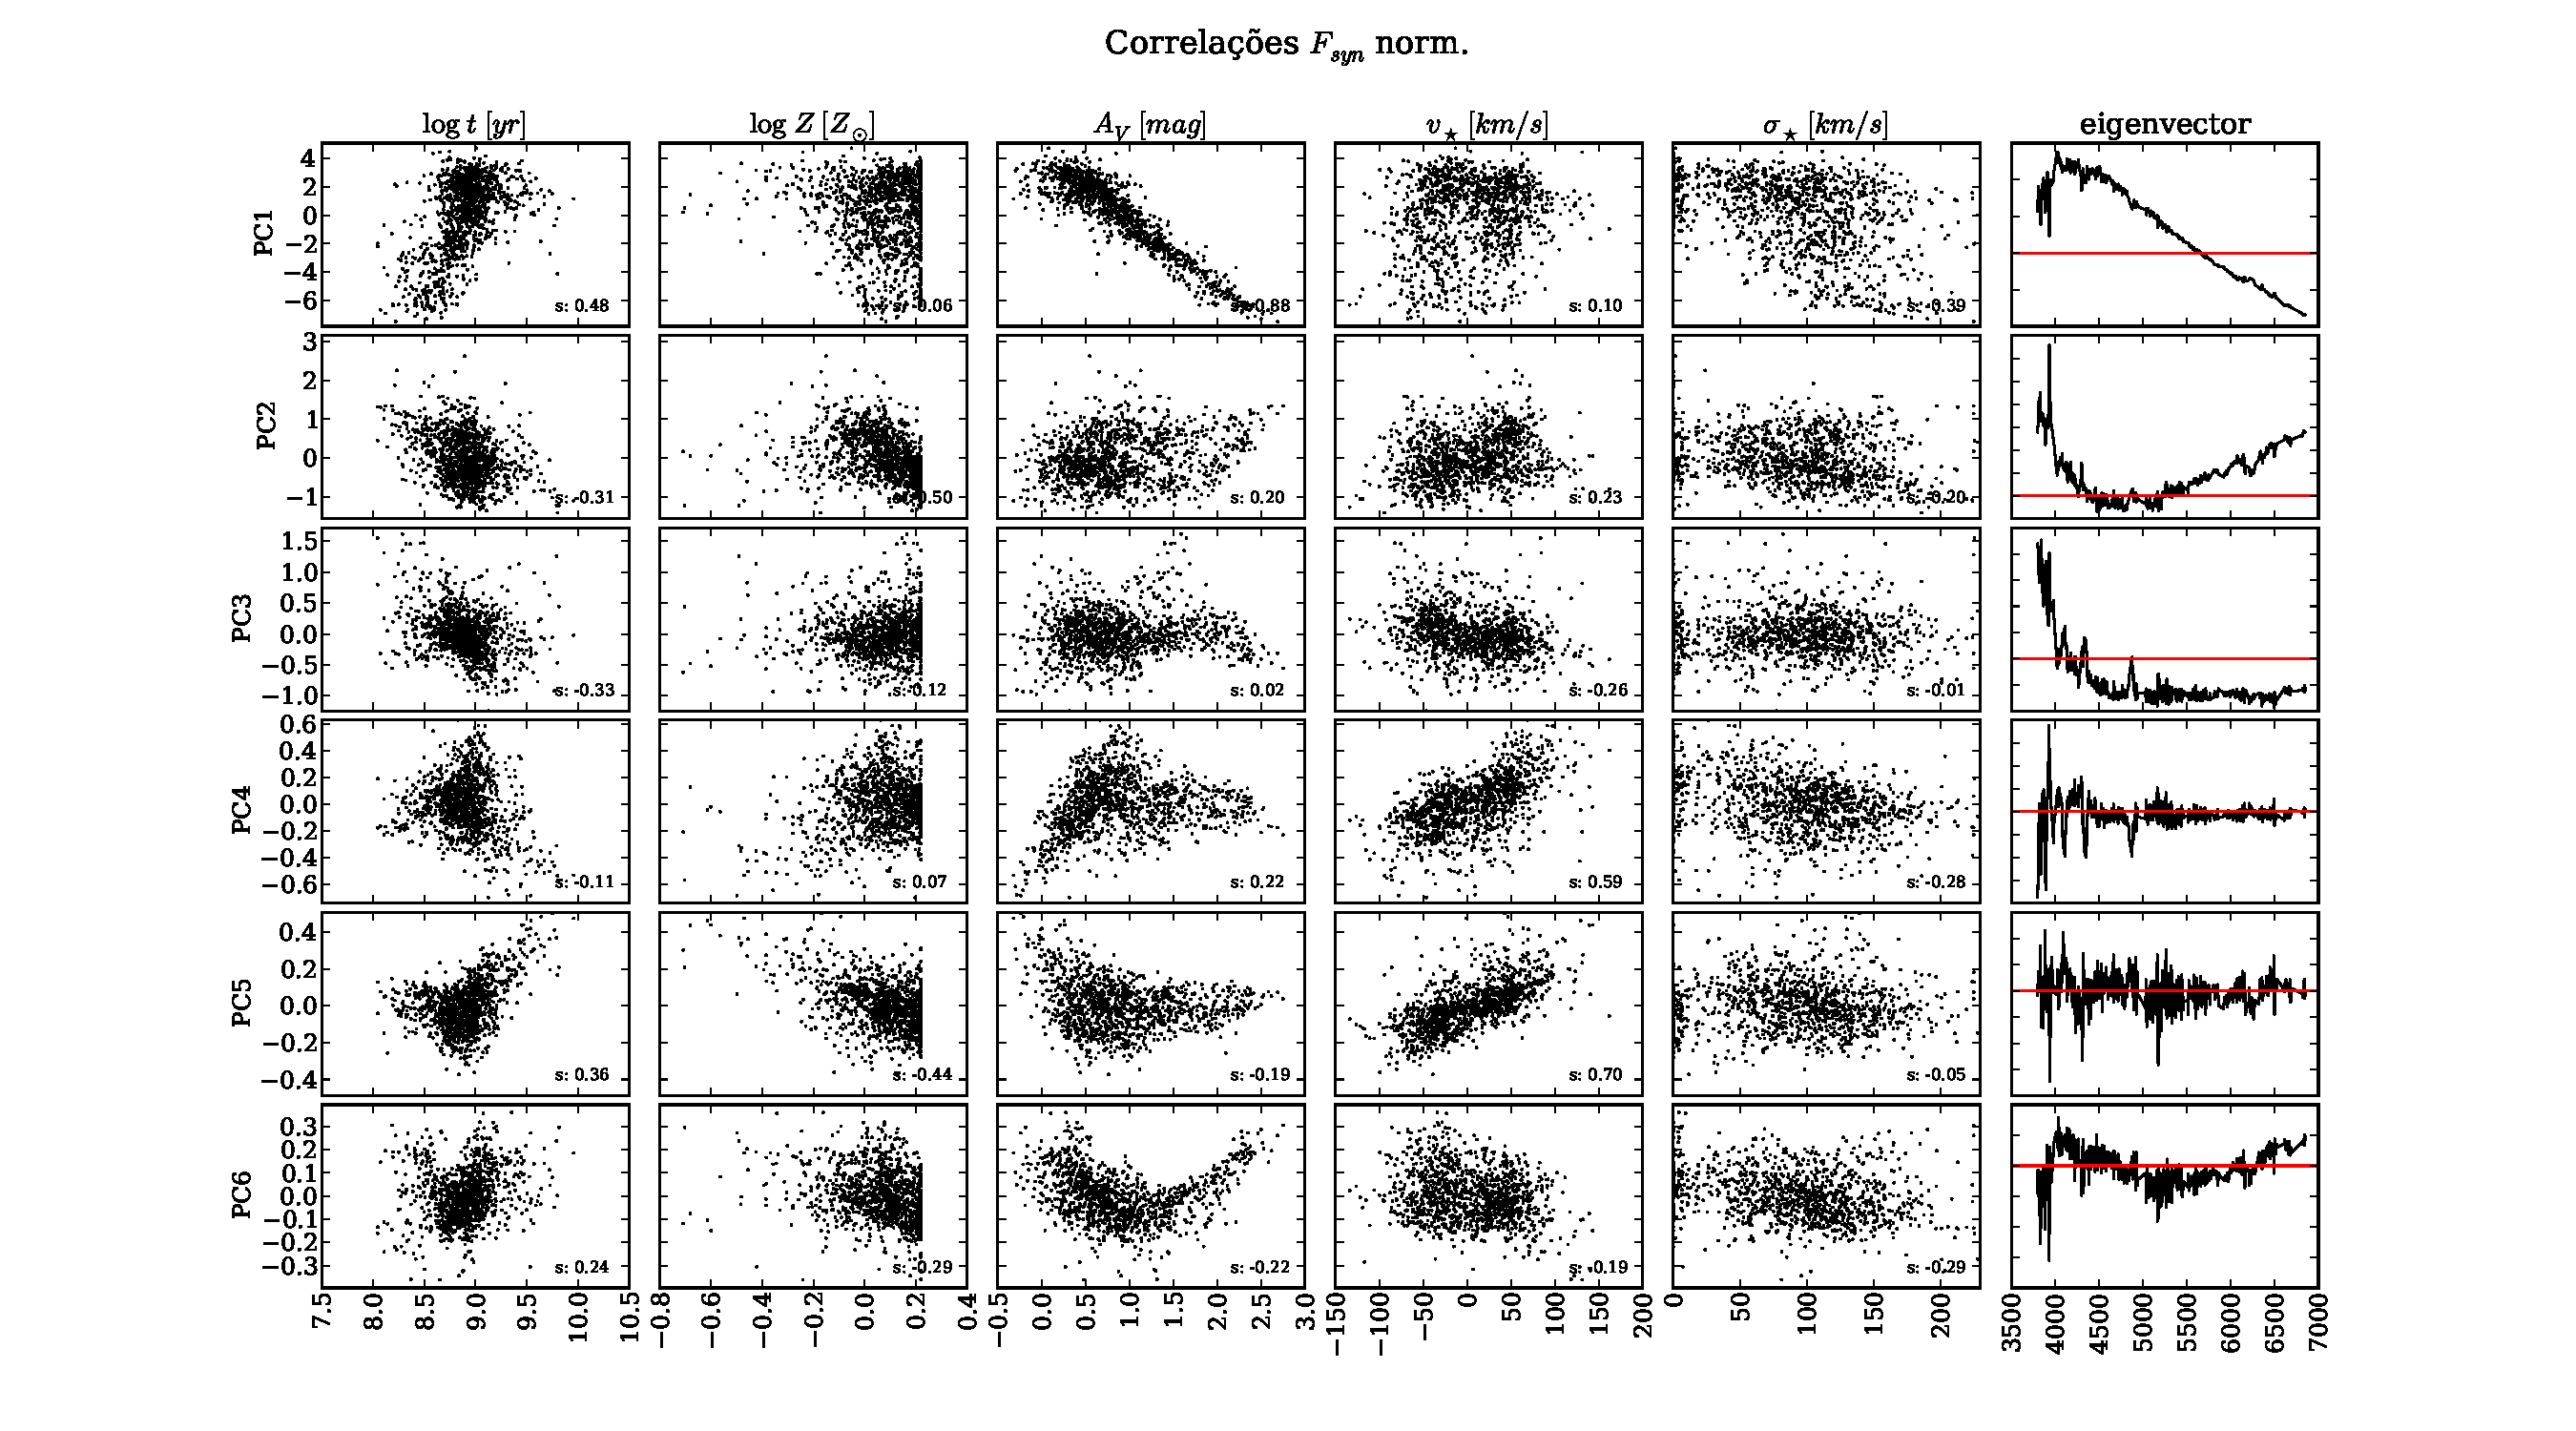
\includegraphics[width=1.2\textwidth, angle=-90]{figuras/K0802-correl-f_syn_norm-PCvsPhys.pdf}
	\caption[Correlações PCs vs. par\^ametros f\'isicos - $f_{syn}$ - ARP 220.]
	{Igual a Figura \ref{fig:K0008correfsynnorm} para a galáxia ARP 220.}
    \label{fig:K0802correfsynnorm}
\end{figure}

\section{Considerações gerais}

Nesse capítulo exploramos algumas galáxias do CALIFA utilizando a Tomografia PCA para os espectros, observados e
sintéticos, normalizados. Fomos capazes de encontrar diversas características nas componentes, sejam correlacionadas com
efeitos físicos ou com problemas nos espectros originais.

Os {\em scree tests} mostram um comportamento assintótico semelhante em todos os casos, com a informação em variância
mais comprimida nas primeiras PCs para o caso $F_{obs}$, seguido por $f_{syn}$ e $f_{obs}$. Cabe aqui ressaltar que mesmo com
o mesmo comportamento assintótico, o número de componentes que ``explicam'' cada galáxia difere muito. Podemos ver isso
na Tabela \ref{tab:resultLambda} que apresenta a variância acumulada para as 6 primeiras componentes ($\Lambda_6$) e o
número de componentes necessárias para obtermos 90\% da variância acumulada.

\begin{table}
	\caption[Variância acumulada para as galáxias análisadas.]
	{Tabela contendo a variância acumulada pelas 6 primeiras PCs ($\Lambda_6$), o número de componentes necessárias para
	cobrir 90\% da variância acumulada ($k_{90\%}$) e o valor total da soma de todas os autovalores ($\Lambda$). Todos os
	valores são calculados para os casos observado e sintético, ambos normalizados.}
	\begin{tabular}{l c c c c c c r}
		Nome da galáxia & CALIFA ID & $\Lambda_6^{obs}\ [\%]$ & $\Lambda_6^{syn}\ [\%]$ & $k_{90\%}^{obs}$ & $k_{90\%}^{syn}$
		& $\Lambda^{obs}$ & $\Lambda^{syn}$ \\ 
		\midrule
		NGC 2916 & K0277 & 89.01 & 99.81 &  12 & 1 & 14.24 & 12.43 \\
		NGC 0001 & K0008 & 59.61 & 99.15 &  82 & 2 &  5.33 &  2.69 \\
		NGC 0776 & K0073 & 66.24 & 99.53 &  95 & 1 &  8.07 &  4.76 \\
		NGC 4210 & K0518 & 85.90 & 99.80 &  37 & 1 & 10.30 &  7.79 \\
		NGC 1167 & K0119 & 45.79 & 98.47 & 161 & 3 &  3.74 &  1.04 \\
		NGC 6515 & K0864 & 40.31 & 98.80 & 104 & 3 &  2.28 &  0.59 \\
		NGC 2623 & K0213 & 90.79 & 99.90 &   5 & 1 & 15.47 & 13.64 \\
		ARP 220  & K0802 & 79.76 & 99.75 &  40 & 1 & 10.98 &  8.21 \\
	\end{tabular}
	\label{tab:resultLambda}
\end{table}

Muita informação contida nessa tabela ainda necessita ser explorada, mas podemos ver que a soma dos autovalores das PCs
para cada galáxia ($\Lambda$), que é igual a soma da variância de todos os comprimentos de onda através das zonas,
parecem crescer juntamente com a ``complexidade'' da galáxia análisada. A variância acumulada para os casos observado e
sintético parecem confirmar que a informação fica mais comprimida para as primeiras PCs para o segundo caso, em relação
ao primeiro. 

Pelo fato de que o campo do CALIFA engloba $\sim100\%$ da luz da galáxia, as estruturas mapeadas pelos cubos de
espectros são diversas, mas não nos impediram de encontrar certas similaridades nos resultados para diferentes galáxias
com o mesmo tipo morfológico. As galáxias espirais possuem geralmente a PC1 correlacionada com a idade, diferentemente
das {\em early-types}, que geralmente parecem ter sua componente principal fortemente ligada à extinção estelar ($A_V$).
Propriedades cinemáticas aparecem de forma singular, ou composta por mais de uma componente, em todos os casos para
todas as galáxias. Já as correlações com a metalicidade aparecem geralmente misturadas com idade ou extinção.

Cabe aqui também ressaltar que através da Tomografia PCA dessas galáxias pudemos encontrar problemas em alguns espectros
das galáxias NGC 0001 e NGC 4210. Na última delas o problema parece ser um pouco mais sério e mais difícil de se
contornar, mas para a galáxia NGC 0001 podemos realizar novamente a PCA cortando 40 \AA\ do lado azul e 10 \AA\ do lado
vermelho do espectro. Talvez para o caso da NGC 4210 possamos reconstruir os cubos de espectros originais suprimindo
determinandas componentes da forma que foi feita por S09 ao reconstruir o espectro do AGN da galáxia NGC 4736 e também
proposto na Seção \ref{sec:conclusao:futWorks}.

% End of this chapter
